\documentclass[twoside]{book}

% Packages required by doxygen
\usepackage{fixltx2e}
\usepackage{calc}
\usepackage{doxygen}
\usepackage[export]{adjustbox} % also loads graphicx
\usepackage{graphicx}
\usepackage[utf8]{inputenc}
\usepackage{makeidx}
\usepackage{multicol}
\usepackage{multirow}
\PassOptionsToPackage{warn}{textcomp}
\usepackage{textcomp}
\usepackage[nointegrals]{wasysym}
\usepackage[table]{xcolor}

% Font selection
\usepackage[T1]{fontenc}
\usepackage[scaled=.90]{helvet}
\usepackage{courier}
\usepackage{amssymb}
\usepackage{sectsty}
\renewcommand{\familydefault}{\sfdefault}
\allsectionsfont{%
  \fontseries{bc}\selectfont%
  \color{darkgray}%
}
\renewcommand{\DoxyLabelFont}{%
  \fontseries{bc}\selectfont%
  \color{darkgray}%
}
\newcommand{\+}{\discretionary{\mbox{\scriptsize$\hookleftarrow$}}{}{}}

% Page & text layout
\usepackage{geometry}
\geometry{%
  a4paper,%
  top=2.5cm,%
  bottom=2.5cm,%
  left=2.5cm,%
  right=2.5cm%
}
\tolerance=750
\hfuzz=15pt
\hbadness=750
\setlength{\emergencystretch}{15pt}
\setlength{\parindent}{0cm}
\setlength{\parskip}{3ex plus 2ex minus 2ex}
\makeatletter
\renewcommand{\paragraph}{%
  \@startsection{paragraph}{4}{0ex}{-1.0ex}{1.0ex}{%
    \normalfont\normalsize\bfseries\SS@parafont%
  }%
}
\renewcommand{\subparagraph}{%
  \@startsection{subparagraph}{5}{0ex}{-1.0ex}{1.0ex}{%
    \normalfont\normalsize\bfseries\SS@subparafont%
  }%
}
\makeatother

% Headers & footers
\usepackage{fancyhdr}
\pagestyle{fancyplain}
\fancyhead[LE]{\fancyplain{}{\bfseries\thepage}}
\fancyhead[CE]{\fancyplain{}{}}
\fancyhead[RE]{\fancyplain{}{\bfseries\leftmark}}
\fancyhead[LO]{\fancyplain{}{\bfseries\rightmark}}
\fancyhead[CO]{\fancyplain{}{}}
\fancyhead[RO]{\fancyplain{}{\bfseries\thepage}}
\fancyfoot[LE]{\fancyplain{}{}}
\fancyfoot[CE]{\fancyplain{}{}}
\fancyfoot[RE]{\fancyplain{}{\bfseries\scriptsize Generated by Doxygen }}
\fancyfoot[LO]{\fancyplain{}{\bfseries\scriptsize Generated by Doxygen }}
\fancyfoot[CO]{\fancyplain{}{}}
\fancyfoot[RO]{\fancyplain{}{}}
\renewcommand{\footrulewidth}{0.4pt}
\renewcommand{\chaptermark}[1]{%
  \markboth{#1}{}%
}
\renewcommand{\sectionmark}[1]{%
  \markright{\thesection\ #1}%
}

% Indices & bibliography
\usepackage{natbib}
\usepackage[titles]{tocloft}
\setcounter{tocdepth}{3}
\setcounter{secnumdepth}{5}
\makeindex

% Hyperlinks (required, but should be loaded last)
\usepackage{ifpdf}
\ifpdf
  \usepackage[pdftex,pagebackref=true]{hyperref}
\else
  \usepackage[ps2pdf,pagebackref=true]{hyperref}
\fi
\hypersetup{%
  colorlinks=true,%
  linkcolor=blue,%
  citecolor=blue,%
  unicode%
}

% Custom commands
\newcommand{\clearemptydoublepage}{%
  \newpage{\pagestyle{empty}\cleardoublepage}%
}

\usepackage{caption}
\captionsetup{labelsep=space,justification=centering,font={bf},singlelinecheck=off,skip=4pt,position=top}

%===== C O N T E N T S =====

\begin{document}

% Titlepage & ToC
\hypersetup{pageanchor=false,
             bookmarksnumbered=true,
             pdfencoding=unicode
            }
\pagenumbering{alph}
\begin{titlepage}
\vspace*{7cm}
\begin{center}%
{\Large Zumo32\+U4 library }\\
\vspace*{1cm}
{\large Generated by Doxygen 1.8.13}\\
\end{center}
\end{titlepage}
\clearemptydoublepage
\pagenumbering{roman}
\tableofcontents
\clearemptydoublepage
\pagenumbering{arabic}
\hypersetup{pageanchor=true}

%--- Begin generated contents ---
\chapter{Zumo32\+U4 library}
\label{index}\hypertarget{index}{}\label{index_md_README}%
\Hypertarget{index_md_README}%
 Version\+: 1.\+2.\+0~\newline
 Release date\+: 2020-\/09-\/11~\newline
 \href{https://travis-ci.org/pololu/zumo-32u4-arduino-library}{\texttt{ }}~\newline
 \href{http://www.pololu.com/}{\texttt{ www.\+pololu.\+com}}\hypertarget{index_autotoc_md5}{}\doxysection{Summary}\label{index_autotoc_md5}
This is a C++ library for the Arduino IDE that helps access the on-\/board hardware of the Zumo 32U4 robot.

The user\textquotesingle{}s guide for the Zumo 32U4 robot is here\+:

\href{https://www.pololu.com/docs/0J63}{\texttt{ https\+://www.\+pololu.\+com/docs/0\+J63}}\hypertarget{index_autotoc_md6}{}\doxysection{Installing the library}\label{index_autotoc_md6}

\begin{DoxyEnumerate}
\item Download the \href{https://github.com/Alexanderallenbrown/Zumo32U4/archive/refs/heads/main.zip}{\texttt{ library from here}} and decompress it.
\item Rename the folder \char`\"{}zumo-\/32u4-\/arduino-\/library-\/master\char`\"{} to \char`\"{}\+Zumo32\+U4\char`\"{}.
\item Move the \char`\"{}\+Zumo32\+U4\char`\"{} folder into the \char`\"{}libraries\char`\"{} directory inside your Arduino sketchbook directory. You can view your sketchbook location by opening the \char`\"{}\+File\char`\"{} menu and selecting \char`\"{}\+Preferences\char`\"{} in the Arduino IDE. If there is not already a \char`\"{}libraries\char`\"{} folder in that location, you should make the folder yourself.
\item After installing the library, restart the Arduino IDE.
\end{DoxyEnumerate}\hypertarget{index_autotoc_md7}{}\doxysection{Examples}\label{index_autotoc_md7}
Several example sketches are available that show how to use the library. You can access them from the Arduino IDE by opening the \char`\"{}\+File\char`\"{} menu, selecting \char`\"{}\+Examples\char`\"{}, and then selecting \char`\"{}\+Zumo32\+U4\char`\"{}. If you cannot find these examples, the library was probably installed incorrectly and you should retry the installation instructions above.\hypertarget{index_autotoc_md8}{}\doxysection{Classes and functions}\label{index_autotoc_md8}
The main classes and functions provided by the library are listed below\+:


\begin{DoxyItemize}
\item \mbox{\hyperlink{class_zumo32_u4_button_a}{Zumo32\+U4\+ButtonA}}
\item \mbox{\hyperlink{class_zumo32_u4_button_b}{Zumo32\+U4\+ButtonB}}
\item \mbox{\hyperlink{class_zumo32_u4_button_c}{Zumo32\+U4\+ButtonC}}
\item \mbox{\hyperlink{class_zumo32_u4_buzzer}{Zumo32\+U4\+Buzzer}}
\item \mbox{\hyperlink{class_zumo32_u4_encoders}{Zumo32\+U4\+Encoders}}
\item \mbox{\hyperlink{class_zumo32_u4_i_m_u}{Zumo32\+U4\+IMU}}
\item \mbox{\hyperlink{class_zumo32_u4_i_r_pulses}{Zumo32\+U4\+IRPulses}}
\item \mbox{\hyperlink{class_zumo32_u4_l_c_d}{Zumo32\+U4\+LCD}}
\item \mbox{\hyperlink{class_zumo32_u4_line_sensors}{Zumo32\+U4\+Line\+Sensors}}
\item \mbox{\hyperlink{class_zumo32_u4_motors}{Zumo32\+U4\+Motors}}
\item \mbox{\hyperlink{class_zumo32_u4_proximity_sensors}{Zumo32\+U4\+Proximity\+Sensors}}
\item \mbox{\hyperlink{_zumo32_u4_8h_ae6ec5117b26ffaaa1b81c8c8b34426e1}{led\+Red()}}
\item \mbox{\hyperlink{_zumo32_u4_8h_a22e68694b618fe149ed42d76e96597ca}{led\+Green()}}
\item \mbox{\hyperlink{_zumo32_u4_8h_a7528cb14b314ccde63c94049402d01c6}{led\+Yellow()}}
\item \mbox{\hyperlink{_zumo32_u4_8h_acf21c49681fe010784b631551ab921f3}{usb\+Power\+Present()}}
\item \mbox{\hyperlink{_zumo32_u4_8h_a9391e187045f8f5a48546b34b6c6db25}{read\+Battery\+Millivolts()}}
\end{DoxyItemize}\hypertarget{index_autotoc_md9}{}\doxysection{Component libraries}\label{index_autotoc_md9}
This library also includes copies of several other Arduino libraries inside it which are used to help implement the classes and functions above.


\begin{DoxyItemize}
\item \href{https://github.com/pololu/fastgpio-arduino}{\texttt{ Fast\+GPIO}}
\item \href{https://github.com/pololu/pololu-buzzer-arduino}{\texttt{ Pololu\+Buzzer}}
\item \href{https://github.com/pololu/pololu-hd44780-arduino}{\texttt{ Pololu\+HD44780}}
\item \href{https://github.com/pololu/pushbutton-arduino}{\texttt{ Pushbutton}}
\item \href{https://github.com/pololu/qtr-sensors-arduino}{\texttt{ QTRSensors}}
\item \href{https://github.com/pololu/usb-pause-arduino}{\texttt{ USBPause}}
\end{DoxyItemize}

You can use these libraries in your sketch automatically without any extra installation steps and without needing to add any extra {\ttfamily \#include} lines to your sketch.

You should avoid adding extra {\ttfamily \#include} lines such as {\ttfamily \#include \texorpdfstring{$<$}{<}\mbox{\hyperlink{_pushbutton_8h}{Pushbutton.\+h}}\texorpdfstring{$>$}{>}} because then the Arduino IDE might try to use the standalone \mbox{\hyperlink{class_pushbutton}{Pushbutton}} library (if you previously installed it), and it would conflict with the copy of the \mbox{\hyperlink{class_pushbutton}{Pushbutton}} code included in this library. The only {\ttfamily \#include} lines needed to access all features of this library are\+:


\begin{DoxyCode}{0}
\DoxyCodeLine{\textcolor{preprocessor}{\#include <Wire.h>}}
\DoxyCodeLine{\textcolor{preprocessor}{\#include <\mbox{\hyperlink{_zumo32_u4_8h}{Zumo32U4.h}}>}}

\end{DoxyCode}
\hypertarget{index_autotoc_md10}{}\doxysection{Version history}\label{index_autotoc_md10}

\begin{DoxyItemize}
\item 1.\+2.\+0 (2020-\/09-\/11)\+: Added a \mbox{\hyperlink{class_zumo32_u4_i_m_u}{Zumo32\+U4\+IMU}} class that abstracts some details of the inertial sensors and supports different IMU types. The examples have been updated to use this class.
\item 1.\+1.\+4 (2017-\/07-\/17)\+: Fixed a bug that caused errors from the right encoder to be reported as errors from the left encoder.
\item 1.\+1.\+3 (2016-\/10-\/12)\+: Fixed a bug that caused the buzzer\textquotesingle{}s {\ttfamily is\+Playing} method to malfunction sometimes when link time optimization is enabled. Also incorporated some minor fixes to the \mbox{\hyperlink{class_q_t_r_sensors}{QTRSensors}} and LSM303 libraries.
\item 1.\+1.\+2 (2016-\/03-\/14)\+: Updated the Demo example so it can compile in Arduino 1.\+6.\+7.
\item 1.\+1.\+1 (2015-\/09-\/01)\+: Moved the library out of the a-\/star repository into its own repository. Added Demo example.
\item 1.\+1.\+0 (2015-\/05-\/06)\+: Updated Fast\+GPIO to version 1.\+0.\+2. Fixed a bug in \mbox{\hyperlink{class_zumo32_u4_proximity_sensors}{Zumo32\+U4\+Proximity\+Sensors}} where the wrong array length was used. Added five demos\+: Rotation\+Resist, Face\+Uphill, Remote\+Control, Balancing, and Sumo\+Proximity\+Sensors.
\item 1.\+0.\+1 (2015-\/03-\/11)\+: Improve the Buttons example.
\item 1.\+0.\+0 (2015-\/03-\/05)\+: Original release. 
\end{DoxyItemize}
\chapter{Hierarchical Index}
\doxysection{Class Hierarchy}
This inheritance list is sorted roughly, but not completely, alphabetically\+:\begin{DoxyCompactList}
\item \contentsline{section}{L3G}{\pageref{class_l3_g}}{}
\item \contentsline{section}{LSM303}{\pageref{class_l_s_m303}}{}
\item \contentsline{section}{Fast\+GPIO\+::Pin$<$ pin $>$}{\pageref{class_fast_g_p_i_o_1_1_pin}}{}
\item \contentsline{section}{Fast\+GPIO\+::Pin\+Loan$<$ pin $>$}{\pageref{class_fast_g_p_i_o_1_1_pin_loan}}{}
\item \contentsline{section}{Pololu\+Buzzer}{\pageref{class_pololu_buzzer}}{}
\begin{DoxyCompactList}
\item \contentsline{section}{Zumo32\+U4\+Buzzer}{\pageref{class_zumo32_u4_buzzer}}{}
\end{DoxyCompactList}
\item Print\begin{DoxyCompactList}
\item \contentsline{section}{Pololu\+HD44780\+Base}{\pageref{class_pololu_h_d44780_base}}{}
\begin{DoxyCompactList}
\item \contentsline{section}{Pololu\+HD44780}{\pageref{class_pololu_h_d44780}}{}
\item \contentsline{section}{Zumo32\+U4\+LCD}{\pageref{class_zumo32_u4_l_c_d}}{}
\end{DoxyCompactList}
\end{DoxyCompactList}
\item \contentsline{section}{Pushbutton\+Base}{\pageref{class_pushbutton_base}}{}
\begin{DoxyCompactList}
\item \contentsline{section}{Pushbutton}{\pageref{class_pushbutton}}{}
\begin{DoxyCompactList}
\item \contentsline{section}{Zumo32\+U4\+ButtonA}{\pageref{class_zumo32_u4_button_a}}{}
\end{DoxyCompactList}
\item \contentsline{section}{Zumo32\+U4\+ButtonB}{\pageref{class_zumo32_u4_button_b}}{}
\item \contentsline{section}{Zumo32\+U4\+ButtonC}{\pageref{class_zumo32_u4_button_c}}{}
\end{DoxyCompactList}
\item \contentsline{section}{QTRSensors}{\pageref{class_q_t_r_sensors}}{}
\begin{DoxyCompactList}
\item \contentsline{section}{QTRSensors\+Analog}{\pageref{class_q_t_r_sensors_analog}}{}
\item \contentsline{section}{QTRSensors\+RC}{\pageref{class_q_t_r_sensors_r_c}}{}
\begin{DoxyCompactList}
\item \contentsline{section}{Zumo32\+U4\+Line\+Sensors}{\pageref{class_zumo32_u4_line_sensors}}{}
\end{DoxyCompactList}
\end{DoxyCompactList}
\item \contentsline{section}{USBPause}{\pageref{class_u_s_b_pause}}{}
\item \contentsline{section}{L3G\+::vector$<$ T $>$}{\pageref{struct_l3_g_1_1vector}}{}
\item \contentsline{section}{LSM303\+::vector$<$ T $>$}{\pageref{struct_l_s_m303_1_1vector}}{}
\item \contentsline{section}{Zumo32\+U4\+IMU\+::vector$<$ T $>$}{\pageref{struct_zumo32_u4_i_m_u_1_1vector}}{}
\item \contentsline{section}{L3G\+::vector$<$ int16\+\_\+t $>$}{\pageref{struct_l3_g_1_1vector}}{}
\item \contentsline{section}{Zumo32\+U4\+Encoders}{\pageref{class_zumo32_u4_encoders}}{}
\item \contentsline{section}{Zumo32\+U4\+IMU}{\pageref{class_zumo32_u4_i_m_u}}{}
\item \contentsline{section}{Zumo32\+U4\+IRPulses}{\pageref{class_zumo32_u4_i_r_pulses}}{}
\item \contentsline{section}{Zumo32\+U4\+Motors}{\pageref{class_zumo32_u4_motors}}{}
\item \contentsline{section}{Zumo32\+U4\+Proximity\+Sensors}{\pageref{class_zumo32_u4_proximity_sensors}}{}
\end{DoxyCompactList}

\chapter{Class Index}
\doxysection{Class List}
Here are the classes, structs, unions and interfaces with brief descriptions\+:\begin{DoxyCompactList}
\item\contentsline{section}{\mbox{\hyperlink{class_fast_g_p_i_o_1_1_pin}{Fast\+GPIO\+::\+Pin$<$ pin $>$}} }{\pageref{class_fast_g_p_i_o_1_1_pin}}{}
\item\contentsline{section}{\mbox{\hyperlink{class_fast_g_p_i_o_1_1_pin_loan}{Fast\+GPIO\+::\+Pin\+Loan$<$ pin $>$}} }{\pageref{class_fast_g_p_i_o_1_1_pin_loan}}{}
\item\contentsline{section}{\mbox{\hyperlink{class_pololu_buzzer}{Pololu\+Buzzer}} \\*Play beeps and music with the buzzer }{\pageref{class_pololu_buzzer}}{}
\item\contentsline{section}{\mbox{\hyperlink{class_pololu_h_d44780}{Pololu\+HD44780}} \\*Main class for interfacing with the HD44780 LCDs }{\pageref{class_pololu_h_d44780}}{}
\item\contentsline{section}{\mbox{\hyperlink{class_pololu_h_d44780_base}{Pololu\+HD44780\+Base}} \\*General class for handling the HD44780 protocol }{\pageref{class_pololu_h_d44780_base}}{}
\item\contentsline{section}{\mbox{\hyperlink{class_pushbutton}{Pushbutton}} \\*Main class for interfacing with pushbuttons }{\pageref{class_pushbutton}}{}
\item\contentsline{section}{\mbox{\hyperlink{class_pushbutton_base}{Pushbutton\+Base}} \\*General pushbutton class that handles debouncing }{\pageref{class_pushbutton_base}}{}
\item\contentsline{section}{\mbox{\hyperlink{class_q_t_r_sensors}{QTRSensors}} }{\pageref{class_q_t_r_sensors}}{}
\item\contentsline{section}{\mbox{\hyperlink{class_q_t_r_sensors_analog}{QTRSensors\+Analog}} }{\pageref{class_q_t_r_sensors_analog}}{}
\item\contentsline{section}{\mbox{\hyperlink{class_q_t_r_sensors_r_c}{QTRSensors\+RC}} }{\pageref{class_q_t_r_sensors_r_c}}{}
\item\contentsline{section}{\mbox{\hyperlink{class_u_s_b_pause}{USBPause}} }{\pageref{class_u_s_b_pause}}{}
\item\contentsline{section}{\mbox{\hyperlink{struct_zumo32_u4_i_m_u_1_1vector}{Zumo32\+U4\+IMU\+::vector$<$ T $>$}} \\*Represents a 3-\/dimensional vector with x, y, and z components }{\pageref{struct_zumo32_u4_i_m_u_1_1vector}}{}
\item\contentsline{section}{\mbox{\hyperlink{class_zumo32_u4_button_a}{Zumo32\+U4\+ButtonA}} \\*Interfaces with button A on the Zumo 32U4 }{\pageref{class_zumo32_u4_button_a}}{}
\item\contentsline{section}{\mbox{\hyperlink{class_zumo32_u4_button_b}{Zumo32\+U4\+ButtonB}} \\*Interfaces with button B on the Zumo 32U4 }{\pageref{class_zumo32_u4_button_b}}{}
\item\contentsline{section}{\mbox{\hyperlink{class_zumo32_u4_button_c}{Zumo32\+U4\+ButtonC}} \\*Interfaces with button C on the Zumo 32U4 }{\pageref{class_zumo32_u4_button_c}}{}
\item\contentsline{section}{\mbox{\hyperlink{class_zumo32_u4_buzzer}{Zumo32\+U4\+Buzzer}} \\*Plays beeps and music on the buzzer on the Zumo 32U4 }{\pageref{class_zumo32_u4_buzzer}}{}
\item\contentsline{section}{\mbox{\hyperlink{class_zumo32_u4_encoders}{Zumo32\+U4\+Encoders}} \\*Reads counts from the encoders on the Zumo 32U4 }{\pageref{class_zumo32_u4_encoders}}{}
\item\contentsline{section}{\mbox{\hyperlink{class_zumo32_u4_i_m_u}{Zumo32\+U4\+IMU}} \\*Interfaces with the inertial sensors on the Zumo 32U4 }{\pageref{class_zumo32_u4_i_m_u}}{}
\item\contentsline{section}{\mbox{\hyperlink{class_zumo32_u4_i_r_pulses}{Zumo32\+U4\+IRPulses}} \\*Emits pulses of infrared (IR) light using the IR LEDs on the Zumo 32U4 Main Board }{\pageref{class_zumo32_u4_i_r_pulses}}{}
\item\contentsline{section}{\mbox{\hyperlink{class_zumo32_u4_l_c_d}{Zumo32\+U4\+LCD}} \\*Writes data to the LCD on the Zumo 32U4 }{\pageref{class_zumo32_u4_l_c_d}}{}
\item\contentsline{section}{\mbox{\hyperlink{class_zumo32_u4_line_sensors}{Zumo32\+U4\+Line\+Sensors}} \\*Gets readings from the five down-\/facing line sensors on the front sensor array }{\pageref{class_zumo32_u4_line_sensors}}{}
\item\contentsline{section}{\mbox{\hyperlink{class_zumo32_u4_motors}{Zumo32\+U4\+Motors}} \\*Controls motor speed and direction on the Zumo 32U4 }{\pageref{class_zumo32_u4_motors}}{}
\item\contentsline{section}{\mbox{\hyperlink{class_zumo32_u4_proximity_sensors}{Zumo32\+U4\+Proximity\+Sensors}} \\*Gets readings from the three proximity sensors on the front sensor array }{\pageref{class_zumo32_u4_proximity_sensors}}{}
\end{DoxyCompactList}

\chapter{File Index}
\section{File List}
Here is a list of all documented files with brief descriptions\+:\begin{DoxyCompactList}
\item\contentsline{section}{\hyperlink{_fast_g_p_i_o_8h}{Fast\+G\+P\+I\+O.\+h} }{\pageref{_fast_g_p_i_o_8h}}{}
\item\contentsline{section}{{\bfseries L3\+G.\+cpp} }{\pageref{_l3_g_8cpp}}{}
\item\contentsline{section}{{\bfseries L3\+G.\+h} }{\pageref{_l3_g_8h}}{}
\item\contentsline{section}{{\bfseries L\+S\+M303.\+cpp} }{\pageref{_l_s_m303_8cpp}}{}
\item\contentsline{section}{{\bfseries L\+S\+M303.\+h} }{\pageref{_l_s_m303_8h}}{}
\item\contentsline{section}{{\bfseries Pololu\+Buzzer.\+cpp} }{\pageref{_pololu_buzzer_8cpp}}{}
\item\contentsline{section}{\hyperlink{_pololu_buzzer_8h}{Pololu\+Buzzer.\+h} }{\pageref{_pololu_buzzer_8h}}{}
\item\contentsline{section}{{\bfseries Pololu\+H\+D44780.\+cpp} }{\pageref{_pololu_h_d44780_8cpp}}{}
\item\contentsline{section}{\hyperlink{_pololu_h_d44780_8h}{Pololu\+H\+D44780.\+h} }{\pageref{_pololu_h_d44780_8h}}{}
\item\contentsline{section}{{\bfseries Pushbutton.\+cpp} }{\pageref{_pushbutton_8cpp}}{}
\item\contentsline{section}{\hyperlink{_pushbutton_8h}{Pushbutton.\+h} }{\pageref{_pushbutton_8h}}{}
\item\contentsline{section}{{\bfseries Q\+T\+R\+Sensors.\+cpp} }{\pageref{_q_t_r_sensors_8cpp}}{}
\item\contentsline{section}{{\bfseries Q\+T\+R\+Sensors.\+h} }{\pageref{_q_t_r_sensors_8h}}{}
\item\contentsline{section}{\hyperlink{_u_s_b_pause_8h}{U\+S\+B\+Pause.\+h} }{\pageref{_u_s_b_pause_8h}}{}
\item\contentsline{section}{\hyperlink{_zumo32_u4_8h}{Zumo32\+U4.\+h} \\*Main header file for the Zumo32\+U4 library }{\pageref{_zumo32_u4_8h}}{}
\item\contentsline{section}{\hyperlink{_zumo32_u4_buttons_8h}{Zumo32\+U4\+Buttons.\+h} }{\pageref{_zumo32_u4_buttons_8h}}{}
\item\contentsline{section}{\hyperlink{_zumo32_u4_buzzer_8h}{Zumo32\+U4\+Buzzer.\+h} }{\pageref{_zumo32_u4_buzzer_8h}}{}
\item\contentsline{section}{{\bfseries Zumo32\+U4\+Encoders.\+cpp} }{\pageref{_zumo32_u4_encoders_8cpp}}{}
\item\contentsline{section}{\hyperlink{_zumo32_u4_encoders_8h}{Zumo32\+U4\+Encoders.\+h} }{\pageref{_zumo32_u4_encoders_8h}}{}
\item\contentsline{section}{{\bfseries Zumo32\+U4\+I\+M\+U.\+cpp} }{\pageref{_zumo32_u4_i_m_u_8cpp}}{}
\item\contentsline{section}{\hyperlink{_zumo32_u4_i_m_u_8h}{Zumo32\+U4\+I\+M\+U.\+h} }{\pageref{_zumo32_u4_i_m_u_8h}}{}
\item\contentsline{section}{{\bfseries Zumo32\+U4\+I\+R\+Pulses.\+cpp} }{\pageref{_zumo32_u4_i_r_pulses_8cpp}}{}
\item\contentsline{section}{\hyperlink{_zumo32_u4_i_r_pulses_8h}{Zumo32\+U4\+I\+R\+Pulses.\+h} }{\pageref{_zumo32_u4_i_r_pulses_8h}}{}
\item\contentsline{section}{\hyperlink{_zumo32_u4_l_c_d_8h}{Zumo32\+U4\+L\+C\+D.\+h} }{\pageref{_zumo32_u4_l_c_d_8h}}{}
\item\contentsline{section}{\hyperlink{_zumo32_u4_line_sensors_8h}{Zumo32\+U4\+Line\+Sensors.\+h} }{\pageref{_zumo32_u4_line_sensors_8h}}{}
\item\contentsline{section}{{\bfseries Zumo32\+U4\+Motors.\+cpp} }{\pageref{_zumo32_u4_motors_8cpp}}{}
\item\contentsline{section}{\hyperlink{_zumo32_u4_motors_8h}{Zumo32\+U4\+Motors.\+h} }{\pageref{_zumo32_u4_motors_8h}}{}
\item\contentsline{section}{{\bfseries Zumo32\+U4\+Proximity\+Sensors.\+cpp} }{\pageref{_zumo32_u4_proximity_sensors_8cpp}}{}
\item\contentsline{section}{\hyperlink{_zumo32_u4_proximity_sensors_8h}{Zumo32\+U4\+Proximity\+Sensors.\+h} }{\pageref{_zumo32_u4_proximity_sensors_8h}}{}
\end{DoxyCompactList}

\chapter{Class Documentation}
\hypertarget{class_fast_g_p_i_o_1_1_pin}{}\doxysection{Fast\+GPIO\+::Pin\texorpdfstring{$<$}{<} pin \texorpdfstring{$>$}{>} Class Template Reference}
\label{class_fast_g_p_i_o_1_1_pin}\index{FastGPIO::Pin$<$ pin $>$@{FastGPIO::Pin$<$ pin $>$}}


{\ttfamily \#include $<$Fast\+GPIO.\+h$>$}

\doxysubsection*{Static Public Member Functions}
\begin{DoxyCompactItemize}
\item 
static void \mbox{\hyperlink{class_fast_g_p_i_o_1_1_pin_a557f119d37b84f3f521d7cbd4cc27b21}{set\+Output\+Low}} () \+\_\+\+\_\+attribute\+\_\+\+\_\+((always\+\_\+inline))
\begin{DoxyCompactList}\small\item\em Configures the pin to be an output driving low. \end{DoxyCompactList}\item 
static void \mbox{\hyperlink{class_fast_g_p_i_o_1_1_pin_aaa0032dcb76492716f477d60721a0579}{set\+Output\+High}} () \+\_\+\+\_\+attribute\+\_\+\+\_\+((always\+\_\+inline))
\begin{DoxyCompactList}\small\item\em Configures the pin to be an output driving high. \end{DoxyCompactList}\item 
static void \mbox{\hyperlink{class_fast_g_p_i_o_1_1_pin_abbdcf0314f4e11543b70ff3a8f63bbb1}{set\+Output\+Toggle}} () \+\_\+\+\_\+attribute\+\_\+\+\_\+((always\+\_\+inline))
\begin{DoxyCompactList}\small\item\em Configures the pin to be an output and toggles it. \end{DoxyCompactList}\item 
static void \mbox{\hyperlink{class_fast_g_p_i_o_1_1_pin_a87fb88b3ea6343db0e4a06f579a10249}{set\+Output}} (bool value) \+\_\+\+\_\+attribute\+\_\+\+\_\+((always\+\_\+inline))
\begin{DoxyCompactList}\small\item\em Sets the pin as an output. \end{DoxyCompactList}\item 
static void \mbox{\hyperlink{class_fast_g_p_i_o_1_1_pin_acff357765bbc7c56564a871d1bdd4868}{set\+Output\+Value\+Low}} () \+\_\+\+\_\+attribute\+\_\+\+\_\+((always\+\_\+inline))
\begin{DoxyCompactList}\small\item\em Sets the output value of the pin to 0. \end{DoxyCompactList}\item 
static void \mbox{\hyperlink{class_fast_g_p_i_o_1_1_pin_a69cae733ab5c400afbb2d731aa31f5f5}{set\+Output\+Value\+High}} () \+\_\+\+\_\+attribute\+\_\+\+\_\+((always\+\_\+inline))
\begin{DoxyCompactList}\small\item\em Sets the output value of the pin to 1. \end{DoxyCompactList}\item 
static void \mbox{\hyperlink{class_fast_g_p_i_o_1_1_pin_a588d0cdd8971e9a6a6939704b227f299}{set\+Output\+Value\+Toggle}} () \+\_\+\+\_\+attribute\+\_\+\+\_\+((always\+\_\+inline))
\begin{DoxyCompactList}\small\item\em Toggles the output value of the pin. \end{DoxyCompactList}\item 
static void \mbox{\hyperlink{class_fast_g_p_i_o_1_1_pin_a2caa56e4e3691227794a39f4b233eb67}{set\+Output\+Value}} (bool value) \+\_\+\+\_\+attribute\+\_\+\+\_\+((always\+\_\+inline))
\begin{DoxyCompactList}\small\item\em Sets the output value of the pin. \end{DoxyCompactList}\item 
static void \mbox{\hyperlink{class_fast_g_p_i_o_1_1_pin_a7f9c4ab269f04bb1ae022b4d7eed3413}{set\+Input}} () \+\_\+\+\_\+attribute\+\_\+\+\_\+((always\+\_\+inline))
\begin{DoxyCompactList}\small\item\em Sets a pin to be a digital input with the internal pull-\/up resistor disabled. \end{DoxyCompactList}\item 
static void \mbox{\hyperlink{class_fast_g_p_i_o_1_1_pin_a32eadc02b421b9b7fc92807bb3304f6e}{set\+Input\+Pulled\+Up}} () \+\_\+\+\_\+attribute\+\_\+\+\_\+((always\+\_\+inline))
\begin{DoxyCompactList}\small\item\em Sets a pin to be a digital input with the internal pull-\/up resistor enabled. \end{DoxyCompactList}\item 
static bool \mbox{\hyperlink{class_fast_g_p_i_o_1_1_pin_acbc38591335717f3feeed14f53b7b79c}{is\+Input\+High}} () \+\_\+\+\_\+attribute\+\_\+\+\_\+((always\+\_\+inline))
\begin{DoxyCompactList}\small\item\em Reads the input value of the pin. \end{DoxyCompactList}\item 
static bool \mbox{\hyperlink{class_fast_g_p_i_o_1_1_pin_ae068011f1d705b9f8f889b32c4b315b3}{is\+Output}} () \+\_\+\+\_\+attribute\+\_\+\+\_\+((always\+\_\+inline))
\begin{DoxyCompactList}\small\item\em Returns 1 if the pin is configured as an output. \end{DoxyCompactList}\item 
static bool \mbox{\hyperlink{class_fast_g_p_i_o_1_1_pin_a28b30134fd55972feb708f07ec8104b7}{is\+Output\+Value\+High}} () \+\_\+\+\_\+attribute\+\_\+\+\_\+((always\+\_\+inline))
\begin{DoxyCompactList}\small\item\em Returns the output value of the pin. \end{DoxyCompactList}\item 
static uint8\+\_\+t \mbox{\hyperlink{class_fast_g_p_i_o_1_1_pin_a79035949bafe62634210dd41486dba2c}{get\+State}} ()
\begin{DoxyCompactList}\small\item\em Returns the full 2-\/bit state of the pin. \end{DoxyCompactList}\item 
static void \mbox{\hyperlink{class_fast_g_p_i_o_1_1_pin_a6dae3821c6b8bcf9f3b7ac2e5114692c}{set\+State}} (uint8\+\_\+t state)
\begin{DoxyCompactList}\small\item\em Sets the full 2-\/bit state of the pin. \end{DoxyCompactList}\end{DoxyCompactItemize}


\doxysubsection{Detailed Description}
\subsubsection*{template$<$uint8\+\_\+t pin$>$\newline
class Fast\+GPIO\+::\+Pin$<$ pin $>$}

\begin{DoxyTemplParams}{Template Parameters}
{\em pin} & The pin number\\
\hline
\end{DoxyTemplParams}
The \mbox{\hyperlink{class_fast_g_p_i_o_1_1_pin}{Fast\+GPIO\+::\+Pin}} class provides static functions for manipulating pins. This class can only be used if the pin number is known at compile time, which means it does not come from a variable that might change and it does not come from the result of a complicated calculation.

Here is some example code showing how to use this class to blink an LED\+:


\begin{DoxyCode}{0}
\DoxyCodeLine{\textcolor{preprocessor}{\#include <\mbox{\hyperlink{_fast_g_p_i_o_8h}{FastGPIO.h}}>}}
\DoxyCodeLine{}
\DoxyCodeLine{\textcolor{preprocessor}{\#define LED\_PIN 13}}
\DoxyCodeLine{}
\DoxyCodeLine{\textcolor{keywordtype}{void} setup() \{}
\DoxyCodeLine{\}}
\DoxyCodeLine{}
\DoxyCodeLine{\textcolor{keywordtype}{void} loop() \{}
\DoxyCodeLine{  \mbox{\hyperlink{class_fast_g_p_i_o_1_1_pin_a87fb88b3ea6343db0e4a06f579a10249}{FastGPIO::Pin<LED\_PIN>::setOutput}}(0);}
\DoxyCodeLine{  delay(500);}
\DoxyCodeLine{  \mbox{\hyperlink{class_fast_g_p_i_o_1_1_pin_a87fb88b3ea6343db0e4a06f579a10249}{FastGPIO::Pin<LED\_PIN>::setOutput}}(1);}
\DoxyCodeLine{  delay(500);}
\DoxyCodeLine{\}}

\end{DoxyCode}
 

Definition at line \mbox{\hyperlink{_fast_g_p_i_o_8h_source_l00275}{275}} of file \mbox{\hyperlink{_fast_g_p_i_o_8h_source}{Fast\+GPIO.\+h}}.



\doxysubsection{Member Function Documentation}
\mbox{\Hypertarget{class_fast_g_p_i_o_1_1_pin_a79035949bafe62634210dd41486dba2c}\label{class_fast_g_p_i_o_1_1_pin_a79035949bafe62634210dd41486dba2c}} 
\index{FastGPIO::Pin$<$ pin $>$@{FastGPIO::Pin$<$ pin $>$}!getState@{getState}}
\index{getState@{getState}!FastGPIO::Pin$<$ pin $>$@{FastGPIO::Pin$<$ pin $>$}}
\doxysubsubsection{\texorpdfstring{getState()}{getState()}}
{\footnotesize\ttfamily template$<$uint8\+\_\+t pin$>$ \\
static uint8\+\_\+t \mbox{\hyperlink{class_fast_g_p_i_o_1_1_pin}{Fast\+GPIO\+::\+Pin}}$<$ pin $>$\+::get\+State (\begin{DoxyParamCaption}{ }\end{DoxyParamCaption})\hspace{0.3cm}{\ttfamily [inline]}, {\ttfamily [static]}}



Returns the full 2-\/bit state of the pin. 

Bit 0 of this function\textquotesingle{}s return value is the pin\textquotesingle{}s output value. Bit 1 of the return value is the pin direction; a value of 1 means output. All the other bits are zero. 

Definition at line \mbox{\hyperlink{_fast_g_p_i_o_8h_source_l00454}{454}} of file \mbox{\hyperlink{_fast_g_p_i_o_8h_source}{Fast\+GPIO.\+h}}.

\mbox{\Hypertarget{class_fast_g_p_i_o_1_1_pin_acbc38591335717f3feeed14f53b7b79c}\label{class_fast_g_p_i_o_1_1_pin_acbc38591335717f3feeed14f53b7b79c}} 
\index{FastGPIO::Pin$<$ pin $>$@{FastGPIO::Pin$<$ pin $>$}!isInputHigh@{isInputHigh}}
\index{isInputHigh@{isInputHigh}!FastGPIO::Pin$<$ pin $>$@{FastGPIO::Pin$<$ pin $>$}}
\doxysubsubsection{\texorpdfstring{isInputHigh()}{isInputHigh()}}
{\footnotesize\ttfamily template$<$uint8\+\_\+t pin$>$ \\
static bool \mbox{\hyperlink{class_fast_g_p_i_o_1_1_pin}{Fast\+GPIO\+::\+Pin}}$<$ pin $>$\+::is\+Input\+High (\begin{DoxyParamCaption}{ }\end{DoxyParamCaption})\hspace{0.3cm}{\ttfamily [inline]}, {\ttfamily [static]}}



Reads the input value of the pin. 

\begin{DoxyReturn}{Returns}
0 if the pin is low, 1 if the pin is high. 
\end{DoxyReturn}


Definition at line \mbox{\hyperlink{_fast_g_p_i_o_8h_source_l00410}{410}} of file \mbox{\hyperlink{_fast_g_p_i_o_8h_source}{Fast\+GPIO.\+h}}.

\mbox{\Hypertarget{class_fast_g_p_i_o_1_1_pin_ae068011f1d705b9f8f889b32c4b315b3}\label{class_fast_g_p_i_o_1_1_pin_ae068011f1d705b9f8f889b32c4b315b3}} 
\index{FastGPIO::Pin$<$ pin $>$@{FastGPIO::Pin$<$ pin $>$}!isOutput@{isOutput}}
\index{isOutput@{isOutput}!FastGPIO::Pin$<$ pin $>$@{FastGPIO::Pin$<$ pin $>$}}
\doxysubsubsection{\texorpdfstring{isOutput()}{isOutput()}}
{\footnotesize\ttfamily template$<$uint8\+\_\+t pin$>$ \\
static bool \mbox{\hyperlink{class_fast_g_p_i_o_1_1_pin}{Fast\+GPIO\+::\+Pin}}$<$ pin $>$\+::is\+Output (\begin{DoxyParamCaption}{ }\end{DoxyParamCaption})\hspace{0.3cm}{\ttfamily [inline]}, {\ttfamily [static]}}



Returns 1 if the pin is configured as an output. 

\begin{DoxyReturn}{Returns}
1 if the pin is an output, 0 if it is an input. 
\end{DoxyReturn}


Definition at line \mbox{\hyperlink{_fast_g_p_i_o_8h_source_l00432}{432}} of file \mbox{\hyperlink{_fast_g_p_i_o_8h_source}{Fast\+GPIO.\+h}}.

\mbox{\Hypertarget{class_fast_g_p_i_o_1_1_pin_a28b30134fd55972feb708f07ec8104b7}\label{class_fast_g_p_i_o_1_1_pin_a28b30134fd55972feb708f07ec8104b7}} 
\index{FastGPIO::Pin$<$ pin $>$@{FastGPIO::Pin$<$ pin $>$}!isOutputValueHigh@{isOutputValueHigh}}
\index{isOutputValueHigh@{isOutputValueHigh}!FastGPIO::Pin$<$ pin $>$@{FastGPIO::Pin$<$ pin $>$}}
\doxysubsubsection{\texorpdfstring{isOutputValueHigh()}{isOutputValueHigh()}}
{\footnotesize\ttfamily template$<$uint8\+\_\+t pin$>$ \\
static bool \mbox{\hyperlink{class_fast_g_p_i_o_1_1_pin}{Fast\+GPIO\+::\+Pin}}$<$ pin $>$\+::is\+Output\+Value\+High (\begin{DoxyParamCaption}{ }\end{DoxyParamCaption})\hspace{0.3cm}{\ttfamily [inline]}, {\ttfamily [static]}}



Returns the output value of the pin. 

This is mainly intended to be called on pins that have been configured an an output. If it is called on an input pin, the return value indicates whether the pull-\/up resistor is enabled or not. 

Definition at line \mbox{\hyperlink{_fast_g_p_i_o_8h_source_l00443}{443}} of file \mbox{\hyperlink{_fast_g_p_i_o_8h_source}{Fast\+GPIO.\+h}}.

\mbox{\Hypertarget{class_fast_g_p_i_o_1_1_pin_a7f9c4ab269f04bb1ae022b4d7eed3413}\label{class_fast_g_p_i_o_1_1_pin_a7f9c4ab269f04bb1ae022b4d7eed3413}} 
\index{FastGPIO::Pin$<$ pin $>$@{FastGPIO::Pin$<$ pin $>$}!setInput@{setInput}}
\index{setInput@{setInput}!FastGPIO::Pin$<$ pin $>$@{FastGPIO::Pin$<$ pin $>$}}
\doxysubsubsection{\texorpdfstring{setInput()}{setInput()}}
{\footnotesize\ttfamily template$<$uint8\+\_\+t pin$>$ \\
static void \mbox{\hyperlink{class_fast_g_p_i_o_1_1_pin}{Fast\+GPIO\+::\+Pin}}$<$ pin $>$\+::set\+Input (\begin{DoxyParamCaption}{ }\end{DoxyParamCaption})\hspace{0.3cm}{\ttfamily [inline]}, {\ttfamily [static]}}



Sets a pin to be a digital input with the internal pull-\/up resistor disabled. 



Definition at line \mbox{\hyperlink{_fast_g_p_i_o_8h_source_l00391}{391}} of file \mbox{\hyperlink{_fast_g_p_i_o_8h_source}{Fast\+GPIO.\+h}}.

\mbox{\Hypertarget{class_fast_g_p_i_o_1_1_pin_a32eadc02b421b9b7fc92807bb3304f6e}\label{class_fast_g_p_i_o_1_1_pin_a32eadc02b421b9b7fc92807bb3304f6e}} 
\index{FastGPIO::Pin$<$ pin $>$@{FastGPIO::Pin$<$ pin $>$}!setInputPulledUp@{setInputPulledUp}}
\index{setInputPulledUp@{setInputPulledUp}!FastGPIO::Pin$<$ pin $>$@{FastGPIO::Pin$<$ pin $>$}}
\doxysubsubsection{\texorpdfstring{setInputPulledUp()}{setInputPulledUp()}}
{\footnotesize\ttfamily template$<$uint8\+\_\+t pin$>$ \\
static void \mbox{\hyperlink{class_fast_g_p_i_o_1_1_pin}{Fast\+GPIO\+::\+Pin}}$<$ pin $>$\+::set\+Input\+Pulled\+Up (\begin{DoxyParamCaption}{ }\end{DoxyParamCaption})\hspace{0.3cm}{\ttfamily [inline]}, {\ttfamily [static]}}



Sets a pin to be a digital input with the internal pull-\/up resistor enabled. 



Definition at line \mbox{\hyperlink{_fast_g_p_i_o_8h_source_l00400}{400}} of file \mbox{\hyperlink{_fast_g_p_i_o_8h_source}{Fast\+GPIO.\+h}}.

\mbox{\Hypertarget{class_fast_g_p_i_o_1_1_pin_a87fb88b3ea6343db0e4a06f579a10249}\label{class_fast_g_p_i_o_1_1_pin_a87fb88b3ea6343db0e4a06f579a10249}} 
\index{FastGPIO::Pin$<$ pin $>$@{FastGPIO::Pin$<$ pin $>$}!setOutput@{setOutput}}
\index{setOutput@{setOutput}!FastGPIO::Pin$<$ pin $>$@{FastGPIO::Pin$<$ pin $>$}}
\doxysubsubsection{\texorpdfstring{setOutput()}{setOutput()}}
{\footnotesize\ttfamily template$<$uint8\+\_\+t pin$>$ \\
static void \mbox{\hyperlink{class_fast_g_p_i_o_1_1_pin}{Fast\+GPIO\+::\+Pin}}$<$ pin $>$\+::set\+Output (\begin{DoxyParamCaption}\item[{bool}]{value }\end{DoxyParamCaption})\hspace{0.3cm}{\ttfamily [inline]}, {\ttfamily [static]}}



Sets the pin as an output. 


\begin{DoxyParams}{Parameters}
{\em value} & Should be 0, LOW, or false to drive the pin low. Should be 1, HIGH, or true to drive the pin high.\\
\hline
\end{DoxyParams}
The PORT bit is set before the DDR bit to ensure that the output is not accidentally driven to the wrong value during the transition. 

Definition at line \mbox{\hyperlink{_fast_g_p_i_o_8h_source_l00318}{318}} of file \mbox{\hyperlink{_fast_g_p_i_o_8h_source}{Fast\+GPIO.\+h}}.

\mbox{\Hypertarget{class_fast_g_p_i_o_1_1_pin_aaa0032dcb76492716f477d60721a0579}\label{class_fast_g_p_i_o_1_1_pin_aaa0032dcb76492716f477d60721a0579}} 
\index{FastGPIO::Pin$<$ pin $>$@{FastGPIO::Pin$<$ pin $>$}!setOutputHigh@{setOutputHigh}}
\index{setOutputHigh@{setOutputHigh}!FastGPIO::Pin$<$ pin $>$@{FastGPIO::Pin$<$ pin $>$}}
\doxysubsubsection{\texorpdfstring{setOutputHigh()}{setOutputHigh()}}
{\footnotesize\ttfamily template$<$uint8\+\_\+t pin$>$ \\
static void \mbox{\hyperlink{class_fast_g_p_i_o_1_1_pin}{Fast\+GPIO\+::\+Pin}}$<$ pin $>$\+::set\+Output\+High (\begin{DoxyParamCaption}{ }\end{DoxyParamCaption})\hspace{0.3cm}{\ttfamily [inline]}, {\ttfamily [static]}}



Configures the pin to be an output driving high. 

This is equivalent to calling set\+Output with an argument of 1, but it has a simpler implementation which means it is more likely to be compiled down to just 2 assembly instructions. 

Definition at line \mbox{\hyperlink{_fast_g_p_i_o_8h_source_l00296}{296}} of file \mbox{\hyperlink{_fast_g_p_i_o_8h_source}{Fast\+GPIO.\+h}}.

\mbox{\Hypertarget{class_fast_g_p_i_o_1_1_pin_a557f119d37b84f3f521d7cbd4cc27b21}\label{class_fast_g_p_i_o_1_1_pin_a557f119d37b84f3f521d7cbd4cc27b21}} 
\index{FastGPIO::Pin$<$ pin $>$@{FastGPIO::Pin$<$ pin $>$}!setOutputLow@{setOutputLow}}
\index{setOutputLow@{setOutputLow}!FastGPIO::Pin$<$ pin $>$@{FastGPIO::Pin$<$ pin $>$}}
\doxysubsubsection{\texorpdfstring{setOutputLow()}{setOutputLow()}}
{\footnotesize\ttfamily template$<$uint8\+\_\+t pin$>$ \\
static void \mbox{\hyperlink{class_fast_g_p_i_o_1_1_pin}{Fast\+GPIO\+::\+Pin}}$<$ pin $>$\+::set\+Output\+Low (\begin{DoxyParamCaption}{ }\end{DoxyParamCaption})\hspace{0.3cm}{\ttfamily [inline]}, {\ttfamily [static]}}



Configures the pin to be an output driving low. 

This is equivalent to calling set\+Output with an argument of 0, but it has a simpler implementation which means it is more likely to be compiled down to just 2 assembly instructions. 

Definition at line \mbox{\hyperlink{_fast_g_p_i_o_8h_source_l00284}{284}} of file \mbox{\hyperlink{_fast_g_p_i_o_8h_source}{Fast\+GPIO.\+h}}.

\mbox{\Hypertarget{class_fast_g_p_i_o_1_1_pin_abbdcf0314f4e11543b70ff3a8f63bbb1}\label{class_fast_g_p_i_o_1_1_pin_abbdcf0314f4e11543b70ff3a8f63bbb1}} 
\index{FastGPIO::Pin$<$ pin $>$@{FastGPIO::Pin$<$ pin $>$}!setOutputToggle@{setOutputToggle}}
\index{setOutputToggle@{setOutputToggle}!FastGPIO::Pin$<$ pin $>$@{FastGPIO::Pin$<$ pin $>$}}
\doxysubsubsection{\texorpdfstring{setOutputToggle()}{setOutputToggle()}}
{\footnotesize\ttfamily template$<$uint8\+\_\+t pin$>$ \\
static void \mbox{\hyperlink{class_fast_g_p_i_o_1_1_pin}{Fast\+GPIO\+::\+Pin}}$<$ pin $>$\+::set\+Output\+Toggle (\begin{DoxyParamCaption}{ }\end{DoxyParamCaption})\hspace{0.3cm}{\ttfamily [inline]}, {\ttfamily [static]}}



Configures the pin to be an output and toggles it. 



Definition at line \mbox{\hyperlink{_fast_g_p_i_o_8h_source_l00304}{304}} of file \mbox{\hyperlink{_fast_g_p_i_o_8h_source}{Fast\+GPIO.\+h}}.

\mbox{\Hypertarget{class_fast_g_p_i_o_1_1_pin_a2caa56e4e3691227794a39f4b233eb67}\label{class_fast_g_p_i_o_1_1_pin_a2caa56e4e3691227794a39f4b233eb67}} 
\index{FastGPIO::Pin$<$ pin $>$@{FastGPIO::Pin$<$ pin $>$}!setOutputValue@{setOutputValue}}
\index{setOutputValue@{setOutputValue}!FastGPIO::Pin$<$ pin $>$@{FastGPIO::Pin$<$ pin $>$}}
\doxysubsubsection{\texorpdfstring{setOutputValue()}{setOutputValue()}}
{\footnotesize\ttfamily template$<$uint8\+\_\+t pin$>$ \\
static void \mbox{\hyperlink{class_fast_g_p_i_o_1_1_pin}{Fast\+GPIO\+::\+Pin}}$<$ pin $>$\+::set\+Output\+Value (\begin{DoxyParamCaption}\item[{bool}]{value }\end{DoxyParamCaption})\hspace{0.3cm}{\ttfamily [inline]}, {\ttfamily [static]}}



Sets the output value of the pin. 


\begin{DoxyParams}{Parameters}
{\em value} & Should be 0, LOW, or false to drive the pin low. Should be 1, HIGH, or true to drive the pin high.\\
\hline
\end{DoxyParams}
This is mainly intended to be used on pins that have already been configured as an output.

If this function is used on an input pin, it has the effect of toggling setting the state of the input pin\textquotesingle{}s pull-\/up resistor. 

Definition at line \mbox{\hyperlink{_fast_g_p_i_o_8h_source_l00376}{376}} of file \mbox{\hyperlink{_fast_g_p_i_o_8h_source}{Fast\+GPIO.\+h}}.

\mbox{\Hypertarget{class_fast_g_p_i_o_1_1_pin_a69cae733ab5c400afbb2d731aa31f5f5}\label{class_fast_g_p_i_o_1_1_pin_a69cae733ab5c400afbb2d731aa31f5f5}} 
\index{FastGPIO::Pin$<$ pin $>$@{FastGPIO::Pin$<$ pin $>$}!setOutputValueHigh@{setOutputValueHigh}}
\index{setOutputValueHigh@{setOutputValueHigh}!FastGPIO::Pin$<$ pin $>$@{FastGPIO::Pin$<$ pin $>$}}
\doxysubsubsection{\texorpdfstring{setOutputValueHigh()}{setOutputValueHigh()}}
{\footnotesize\ttfamily template$<$uint8\+\_\+t pin$>$ \\
static void \mbox{\hyperlink{class_fast_g_p_i_o_1_1_pin}{Fast\+GPIO\+::\+Pin}}$<$ pin $>$\+::set\+Output\+Value\+High (\begin{DoxyParamCaption}{ }\end{DoxyParamCaption})\hspace{0.3cm}{\ttfamily [inline]}, {\ttfamily [static]}}



Sets the output value of the pin to 1. 

This is mainly intended to be used on pins that have already been configured as an output in order to make the output drive low.

If this is used on an input pin, it has the effect of enabling the input pin\textquotesingle{}s pull-\/up resistor. 

Definition at line \mbox{\hyperlink{_fast_g_p_i_o_8h_source_l00345}{345}} of file \mbox{\hyperlink{_fast_g_p_i_o_8h_source}{Fast\+GPIO.\+h}}.

\mbox{\Hypertarget{class_fast_g_p_i_o_1_1_pin_acff357765bbc7c56564a871d1bdd4868}\label{class_fast_g_p_i_o_1_1_pin_acff357765bbc7c56564a871d1bdd4868}} 
\index{FastGPIO::Pin$<$ pin $>$@{FastGPIO::Pin$<$ pin $>$}!setOutputValueLow@{setOutputValueLow}}
\index{setOutputValueLow@{setOutputValueLow}!FastGPIO::Pin$<$ pin $>$@{FastGPIO::Pin$<$ pin $>$}}
\doxysubsubsection{\texorpdfstring{setOutputValueLow()}{setOutputValueLow()}}
{\footnotesize\ttfamily template$<$uint8\+\_\+t pin$>$ \\
static void \mbox{\hyperlink{class_fast_g_p_i_o_1_1_pin}{Fast\+GPIO\+::\+Pin}}$<$ pin $>$\+::set\+Output\+Value\+Low (\begin{DoxyParamCaption}{ }\end{DoxyParamCaption})\hspace{0.3cm}{\ttfamily [inline]}, {\ttfamily [static]}}



Sets the output value of the pin to 0. 

This is mainly intended to be used on pins that have already been configured as an output in order to make the output drive low.

If this is used on an input pin, it has the effect of disabling the input pin\textquotesingle{}s pull-\/up resistor. 

Definition at line \mbox{\hyperlink{_fast_g_p_i_o_8h_source_l00332}{332}} of file \mbox{\hyperlink{_fast_g_p_i_o_8h_source}{Fast\+GPIO.\+h}}.

\mbox{\Hypertarget{class_fast_g_p_i_o_1_1_pin_a588d0cdd8971e9a6a6939704b227f299}\label{class_fast_g_p_i_o_1_1_pin_a588d0cdd8971e9a6a6939704b227f299}} 
\index{FastGPIO::Pin$<$ pin $>$@{FastGPIO::Pin$<$ pin $>$}!setOutputValueToggle@{setOutputValueToggle}}
\index{setOutputValueToggle@{setOutputValueToggle}!FastGPIO::Pin$<$ pin $>$@{FastGPIO::Pin$<$ pin $>$}}
\doxysubsubsection{\texorpdfstring{setOutputValueToggle()}{setOutputValueToggle()}}
{\footnotesize\ttfamily template$<$uint8\+\_\+t pin$>$ \\
static void \mbox{\hyperlink{class_fast_g_p_i_o_1_1_pin}{Fast\+GPIO\+::\+Pin}}$<$ pin $>$\+::set\+Output\+Value\+Toggle (\begin{DoxyParamCaption}{ }\end{DoxyParamCaption})\hspace{0.3cm}{\ttfamily [inline]}, {\ttfamily [static]}}



Toggles the output value of the pin. 

This is mainly intended to be used on pins that have already been configured as an output. If the pin was driving low, this function changes it to drive high. If the pin was driving high, this function changes it to drive low.

If this function is used on an input pin, it has the effect of toggling the state of the input pin\textquotesingle{}s pull-\/up resistor. 

Definition at line \mbox{\hyperlink{_fast_g_p_i_o_8h_source_l00360}{360}} of file \mbox{\hyperlink{_fast_g_p_i_o_8h_source}{Fast\+GPIO.\+h}}.

\mbox{\Hypertarget{class_fast_g_p_i_o_1_1_pin_a6dae3821c6b8bcf9f3b7ac2e5114692c}\label{class_fast_g_p_i_o_1_1_pin_a6dae3821c6b8bcf9f3b7ac2e5114692c}} 
\index{FastGPIO::Pin$<$ pin $>$@{FastGPIO::Pin$<$ pin $>$}!setState@{setState}}
\index{setState@{setState}!FastGPIO::Pin$<$ pin $>$@{FastGPIO::Pin$<$ pin $>$}}
\doxysubsubsection{\texorpdfstring{setState()}{setState()}}
{\footnotesize\ttfamily template$<$uint8\+\_\+t pin$>$ \\
static void \mbox{\hyperlink{class_fast_g_p_i_o_1_1_pin}{Fast\+GPIO\+::\+Pin}}$<$ pin $>$\+::set\+State (\begin{DoxyParamCaption}\item[{uint8\+\_\+t}]{state }\end{DoxyParamCaption})\hspace{0.3cm}{\ttfamily [inline]}, {\ttfamily [static]}}



Sets the full 2-\/bit state of the pin. 


\begin{DoxyParams}{Parameters}
{\em state} & The state of the pin, as returns from get\+State. All bits other than bits 0 and 1 are ignored.\\
\hline
\end{DoxyParams}
Sometimes this function will need to change both the PORT bit (which specifies the output value) and the DDR bit (which specifies whether the pin is an output). If the DDR bit is getting set to 0, this function changes DDR first, and if it is getting set to 1, this function changes DDR last. This guarantees that the intermediate pin state is always an input state. 

Definition at line \mbox{\hyperlink{_fast_g_p_i_o_8h_source_l00486}{486}} of file \mbox{\hyperlink{_fast_g_p_i_o_8h_source}{Fast\+GPIO.\+h}}.



The documentation for this class was generated from the following file\+:\begin{DoxyCompactItemize}
\item 
\mbox{\hyperlink{_fast_g_p_i_o_8h}{Fast\+GPIO.\+h}}\end{DoxyCompactItemize}

\hypertarget{class_fast_g_p_i_o_1_1_pin_loan}{}\doxysection{Fast\+GPIO\+::Pin\+Loan\texorpdfstring{$<$}{<} pin \texorpdfstring{$>$}{>} Class Template Reference}
\label{class_fast_g_p_i_o_1_1_pin_loan}\index{FastGPIO::PinLoan$<$ pin $>$@{FastGPIO::PinLoan$<$ pin $>$}}


{\ttfamily \#include $<$Fast\+GPIO.\+h$>$}

\doxysubsection*{Public Attributes}
\begin{DoxyCompactItemize}
\item 
uint8\+\_\+t \mbox{\hyperlink{class_fast_g_p_i_o_1_1_pin_loan_a86acee97ba5ecd85d839dc31653e2727}{state}}
\begin{DoxyCompactList}\small\item\em The state of the pin as returned from \mbox{\hyperlink{class_fast_g_p_i_o_1_1_pin_a79035949bafe62634210dd41486dba2c}{Fast\+GPIO\+::\+Pin\+::get\+State}}. \end{DoxyCompactList}\end{DoxyCompactItemize}


\doxysubsection{Detailed Description}
\subsubsection*{template$<$uint8\+\_\+t pin$>$\newline
class Fast\+GPIO\+::\+Pin\+Loan$<$ pin $>$}
This class saves the state of the specified pin in its constructor when it is created, and restores the pin to that state in its destructor. This can be very useful if a pin is being used for multiple purposes. It allows you to write code that temporarily changes the state of the pin and is guaranteed to restore the state later.

For example, if you were controlling both a button and an LED using a single pin and you wanted to see if the button was pressed without affecting the LED, you could write\+:


\begin{DoxyCode}{0}
\DoxyCodeLine{\textcolor{keywordtype}{bool} buttonIsPressed()}
\DoxyCodeLine{\{}
\DoxyCodeLine{    \mbox{\hyperlink{class_fast_g_p_i_o_1_1_pin_loan}{FastGPIO::PinLoan<IO\_D5>}} loan;}
\DoxyCodeLine{    \mbox{\hyperlink{class_fast_g_p_i_o_1_1_pin_a32eadc02b421b9b7fc92807bb3304f6e}{FastGPIO::Pin<IO\_D5>::setInputPulledUp}}();}
\DoxyCodeLine{    \_delay\_us(10);}
\DoxyCodeLine{    \textcolor{keywordflow}{return} !\mbox{\hyperlink{class_fast_g_p_i_o_1_1_pin_acbc38591335717f3feeed14f53b7b79c}{FastGPIO::Pin<IO\_D5>::isInputHigh}}();}
\DoxyCodeLine{\}}

\end{DoxyCode}


This is equivalent to\+:


\begin{DoxyCode}{0}
\DoxyCodeLine{\textcolor{keywordtype}{bool} buttonIsPressed()}
\DoxyCodeLine{\{}
\DoxyCodeLine{    uint8\_t \mbox{\hyperlink{class_fast_g_p_i_o_1_1_pin_loan_a86acee97ba5ecd85d839dc31653e2727}{state}} = \mbox{\hyperlink{class_fast_g_p_i_o_1_1_pin_a79035949bafe62634210dd41486dba2c}{FastGPIO::Pin<IO\_D5>::getState}}();}
\DoxyCodeLine{    \mbox{\hyperlink{class_fast_g_p_i_o_1_1_pin_a32eadc02b421b9b7fc92807bb3304f6e}{FastGPIO::Pin<IO\_D5>::setInputPulledUp}}();}
\DoxyCodeLine{    \_delay\_us(10);}
\DoxyCodeLine{    \textcolor{keywordtype}{bool} value = !\mbox{\hyperlink{class_fast_g_p_i_o_1_1_pin_acbc38591335717f3feeed14f53b7b79c}{FastGPIO::Pin<IO\_D5>::isInputHigh}}();}
\DoxyCodeLine{    \mbox{\hyperlink{class_fast_g_p_i_o_1_1_pin_a6dae3821c6b8bcf9f3b7ac2e5114692c}{FastGPIO::Pin<IO\_D5>::setState}}(\mbox{\hyperlink{class_fast_g_p_i_o_1_1_pin_loan_a86acee97ba5ecd85d839dc31653e2727}{state}});}
\DoxyCodeLine{    \textcolor{keywordflow}{return} value;}
\DoxyCodeLine{\}}

\end{DoxyCode}
 

Definition at line \mbox{\hyperlink{_fast_g_p_i_o_8h_source_l00542}{542}} of file \mbox{\hyperlink{_fast_g_p_i_o_8h_source}{Fast\+GPIO.\+h}}.



\doxysubsection{Constructor \& Destructor Documentation}
\mbox{\Hypertarget{class_fast_g_p_i_o_1_1_pin_loan_a73eca997fe1f8d2d28cfb40fe2368bc0}\label{class_fast_g_p_i_o_1_1_pin_loan_a73eca997fe1f8d2d28cfb40fe2368bc0}} 
\index{FastGPIO::PinLoan$<$ pin $>$@{FastGPIO::PinLoan$<$ pin $>$}!PinLoan@{PinLoan}}
\index{PinLoan@{PinLoan}!FastGPIO::PinLoan$<$ pin $>$@{FastGPIO::PinLoan$<$ pin $>$}}
\doxysubsubsection{\texorpdfstring{PinLoan()}{PinLoan()}}
{\footnotesize\ttfamily template$<$uint8\+\_\+t pin$>$ \\
\mbox{\hyperlink{class_fast_g_p_i_o_1_1_pin_loan}{Fast\+GPIO\+::\+Pin\+Loan}}$<$ pin $>$\+::\+Pin\+Loan (\begin{DoxyParamCaption}{ }\end{DoxyParamCaption})\hspace{0.3cm}{\ttfamily [inline]}}



Definition at line \mbox{\hyperlink{_fast_g_p_i_o_8h_source_l00548}{548}} of file \mbox{\hyperlink{_fast_g_p_i_o_8h_source}{Fast\+GPIO.\+h}}.

\mbox{\Hypertarget{class_fast_g_p_i_o_1_1_pin_loan_a4d5df78a06fa9ffdab565aaf8ff1ebf0}\label{class_fast_g_p_i_o_1_1_pin_loan_a4d5df78a06fa9ffdab565aaf8ff1ebf0}} 
\index{FastGPIO::PinLoan$<$ pin $>$@{FastGPIO::PinLoan$<$ pin $>$}!````~PinLoan@{$\sim$PinLoan}}
\index{````~PinLoan@{$\sim$PinLoan}!FastGPIO::PinLoan$<$ pin $>$@{FastGPIO::PinLoan$<$ pin $>$}}
\doxysubsubsection{\texorpdfstring{$\sim$PinLoan()}{~PinLoan()}}
{\footnotesize\ttfamily template$<$uint8\+\_\+t pin$>$ \\
\mbox{\hyperlink{class_fast_g_p_i_o_1_1_pin_loan}{Fast\+GPIO\+::\+Pin\+Loan}}$<$ pin $>$\+::$\sim$\mbox{\hyperlink{class_fast_g_p_i_o_1_1_pin_loan}{Pin\+Loan}} (\begin{DoxyParamCaption}{ }\end{DoxyParamCaption})\hspace{0.3cm}{\ttfamily [inline]}}



Definition at line \mbox{\hyperlink{_fast_g_p_i_o_8h_source_l00553}{553}} of file \mbox{\hyperlink{_fast_g_p_i_o_8h_source}{Fast\+GPIO.\+h}}.



\doxysubsection{Member Data Documentation}
\mbox{\Hypertarget{class_fast_g_p_i_o_1_1_pin_loan_a86acee97ba5ecd85d839dc31653e2727}\label{class_fast_g_p_i_o_1_1_pin_loan_a86acee97ba5ecd85d839dc31653e2727}} 
\index{FastGPIO::PinLoan$<$ pin $>$@{FastGPIO::PinLoan$<$ pin $>$}!state@{state}}
\index{state@{state}!FastGPIO::PinLoan$<$ pin $>$@{FastGPIO::PinLoan$<$ pin $>$}}
\doxysubsubsection{\texorpdfstring{state}{state}}
{\footnotesize\ttfamily template$<$uint8\+\_\+t pin$>$ \\
uint8\+\_\+t \mbox{\hyperlink{class_fast_g_p_i_o_1_1_pin_loan}{Fast\+GPIO\+::\+Pin\+Loan}}$<$ pin $>$\+::state}



The state of the pin as returned from \mbox{\hyperlink{class_fast_g_p_i_o_1_1_pin_a79035949bafe62634210dd41486dba2c}{Fast\+GPIO\+::\+Pin\+::get\+State}}. 



Definition at line \mbox{\hyperlink{_fast_g_p_i_o_8h_source_l00546}{546}} of file \mbox{\hyperlink{_fast_g_p_i_o_8h_source}{Fast\+GPIO.\+h}}.



The documentation for this class was generated from the following file\+:\begin{DoxyCompactItemize}
\item 
\mbox{\hyperlink{_fast_g_p_i_o_8h}{Fast\+GPIO.\+h}}\end{DoxyCompactItemize}

\hypertarget{class_pololu_buzzer}{}\doxysection{Pololu\+Buzzer Class Reference}
\label{class_pololu_buzzer}\index{PololuBuzzer@{PololuBuzzer}}


Play beeps and music with the buzzer.  




{\ttfamily \#include $<$Pololu\+Buzzer.\+h$>$}

Inheritance diagram for Pololu\+Buzzer\+:\begin{figure}[H]
\begin{center}
\leavevmode
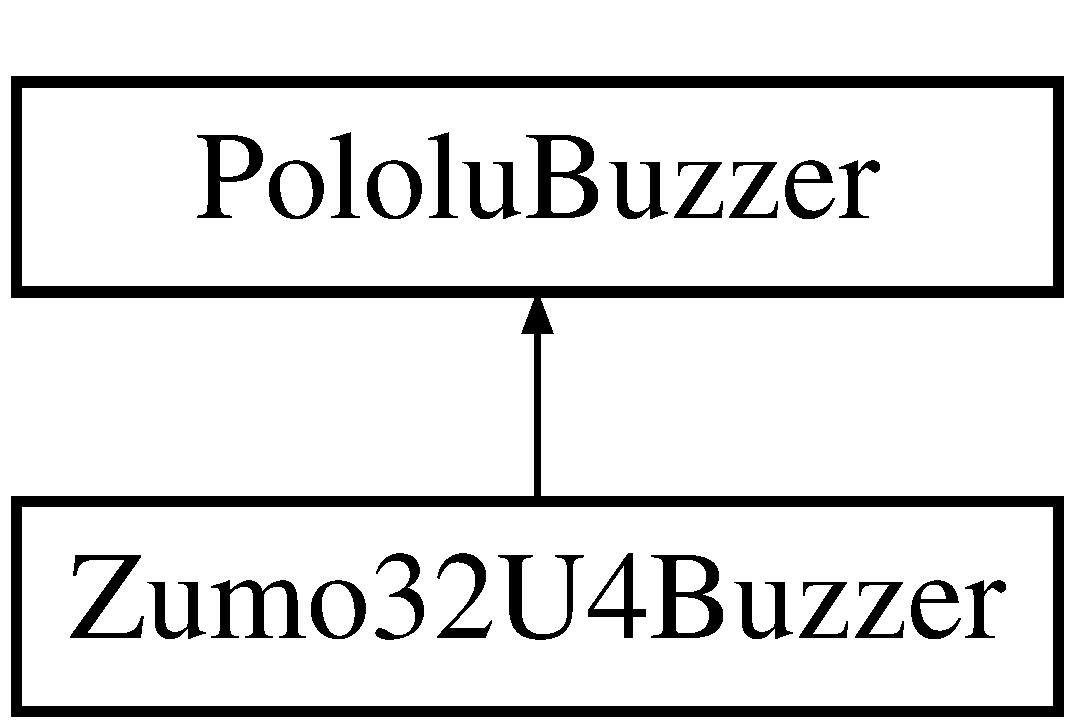
\includegraphics[height=2.000000cm]{class_pololu_buzzer}
\end{center}
\end{figure}
\doxysubsection*{Static Public Member Functions}
\begin{DoxyCompactItemize}
\item 
static void \mbox{\hyperlink{class_pololu_buzzer_a931fafd76045ae59d4ba62c9bf90b0dc}{play\+Frequency}} (unsigned int freq, unsigned int duration, unsigned char volume)
\begin{DoxyCompactList}\small\item\em Plays the specified frequency for the specified duration. \end{DoxyCompactList}\item 
static void \mbox{\hyperlink{class_pololu_buzzer_a989d410dd6cdb7abfa136c3734040fb5}{play\+Note}} (unsigned char note, unsigned int duration, unsigned char volume)
\begin{DoxyCompactList}\small\item\em Plays the specified note for the specified duration. \end{DoxyCompactList}\item 
static void \mbox{\hyperlink{class_pololu_buzzer_a22f45ef7cdf9dc8fc54e617244368277}{play}} (const char $\ast$sequence)
\begin{DoxyCompactList}\small\item\em Plays the specified sequence of notes. \end{DoxyCompactList}\item 
static void \mbox{\hyperlink{class_pololu_buzzer_a07ff4e9d9f7e4f37a58e149640b61f4e}{play\+From\+Program\+Space}} (const char $\ast$sequence)
\begin{DoxyCompactList}\small\item\em Plays the specified sequence of notes from program space. \end{DoxyCompactList}\item 
static void \mbox{\hyperlink{class_pololu_buzzer_ab72bde97ceceef8705f1bbaeccb970db}{play\+Mode}} (unsigned char mode)
\begin{DoxyCompactList}\small\item\em Controls whether {\ttfamily \mbox{\hyperlink{class_pololu_buzzer_a22f45ef7cdf9dc8fc54e617244368277}{play()}}} sequence is played automatically or must be driven with {\ttfamily \mbox{\hyperlink{class_pololu_buzzer_a427225dcc85c1e65078e4397b9890929}{play\+Check()}}}. \end{DoxyCompactList}\item 
static unsigned char \mbox{\hyperlink{class_pololu_buzzer_a427225dcc85c1e65078e4397b9890929}{play\+Check}} ()
\begin{DoxyCompactList}\small\item\em Starts the next note in a sequence, if necessary, in {\ttfamily PLAY\+\_\+\+CHECK} mode. \end{DoxyCompactList}\item 
static unsigned char \mbox{\hyperlink{class_pololu_buzzer_a8045fdf0a144e0b71a5b223a0ef34027}{is\+Playing}} ()
\begin{DoxyCompactList}\small\item\em Checks whether a note, frequency, or sequence is being played. \end{DoxyCompactList}\item 
static void \mbox{\hyperlink{class_pololu_buzzer_a233fe0ffe5f23582b1c55beaa718d527}{stop\+Playing}} ()
\begin{DoxyCompactList}\small\item\em Stops any note, frequency, or melody being played. \end{DoxyCompactList}\end{DoxyCompactItemize}


\doxysubsection{Detailed Description}
Play beeps and music with the buzzer. 

The \mbox{\hyperlink{class_pololu_buzzer}{Pololu\+Buzzer}} library allows various sounds to be played through a buzzer, from simple beeps to complex tunes.

On the ATmega328\+P/168 boards, this library uses Timer 2 and pin 3 (PD3/\+OC2B). On ATmega32\+U4 boards, this library uses Timer 4 and pin 6 (PD7/\+OC4D). This library will conflict will other libraries that use the same timer or pin.

Note durations are timed using a timer overflow interrupt ({\ttfamily TIMER2\+\_\+\+OVF}/{\ttfamily TIMER4\+\_\+\+OVF}), which will briefly interrupt execution of your main program at the frequency of the sound being played. In most cases, the interrupt-\/handling routine is very short (several microseconds). However, when playing a sequence of notes in {\ttfamily PLAY\+\_\+\+AUTOMATIC} mode (the default mode) with the {\ttfamily \mbox{\hyperlink{class_pololu_buzzer_a22f45ef7cdf9dc8fc54e617244368277}{play()}}} command, this interrupt takes much longer than normal (perhaps several hundred microseconds) every time it starts a new note. It is important to take this into account when writing timing-\/critical code.

This library is fully compatible with the Orangutan\+Buzzer functions in the \href{http://www.pololu.com/docs/0J18}{\texttt{ Pololu AVR C/\+C++ Library}} and the \href{https://github.com/pololu/zumo-shield}{\texttt{ Zumo\+Buzzer library}}, so any sequences and melodies written for those libraries will also work with the equivalent \mbox{\hyperlink{class_pololu_buzzer}{Pololu\+Buzzer}} functions. 

Definition at line \mbox{\hyperlink{_pololu_buzzer_8h_source_l00089}{89}} of file \mbox{\hyperlink{_pololu_buzzer_8h_source}{Pololu\+Buzzer.\+h}}.



\doxysubsection{Member Function Documentation}
\mbox{\Hypertarget{class_pololu_buzzer_a8045fdf0a144e0b71a5b223a0ef34027}\label{class_pololu_buzzer_a8045fdf0a144e0b71a5b223a0ef34027}} 
\index{PololuBuzzer@{PololuBuzzer}!isPlaying@{isPlaying}}
\index{isPlaying@{isPlaying}!PololuBuzzer@{PololuBuzzer}}
\doxysubsubsection{\texorpdfstring{isPlaying()}{isPlaying()}}
{\footnotesize\ttfamily unsigned char Pololu\+Buzzer\+::is\+Playing (\begin{DoxyParamCaption}{ }\end{DoxyParamCaption})\hspace{0.3cm}{\ttfamily [static]}}



Checks whether a note, frequency, or sequence is being played. 

\begin{DoxyReturn}{Returns}
1 if the buzzer is current playing a note, frequency, or sequence; 0 otherwise.
\end{DoxyReturn}
This method returns 1 (true) if the buzzer is currently playing a note/frequency or if it is still playing a sequence started by {\ttfamily \mbox{\hyperlink{class_pololu_buzzer_a22f45ef7cdf9dc8fc54e617244368277}{play()}}}. Otherwise, it returns 0 (false). You can poll this method to determine when it\textquotesingle{}s time to play the next note in a sequence, or you can use it as the argument to a delay loop to wait while the buzzer is busy. 

Definition at line \mbox{\hyperlink{_pololu_buzzer_8cpp_source_l00400}{400}} of file \mbox{\hyperlink{_pololu_buzzer_8cpp_source}{Pololu\+Buzzer.\+cpp}}.

\mbox{\Hypertarget{class_pololu_buzzer_a22f45ef7cdf9dc8fc54e617244368277}\label{class_pololu_buzzer_a22f45ef7cdf9dc8fc54e617244368277}} 
\index{PololuBuzzer@{PololuBuzzer}!play@{play}}
\index{play@{play}!PololuBuzzer@{PololuBuzzer}}
\doxysubsubsection{\texorpdfstring{play()}{play()}}
{\footnotesize\ttfamily void Pololu\+Buzzer\+::play (\begin{DoxyParamCaption}\item[{const char $\ast$}]{sequence }\end{DoxyParamCaption})\hspace{0.3cm}{\ttfamily [static]}}



Plays the specified sequence of notes. 


\begin{DoxyParams}{Parameters}
{\em sequence} & Char array containing a sequence of notes to play.\\
\hline
\end{DoxyParams}
If the play mode is {\ttfamily PLAY\+\_\+\+AUTOMATIC} (default), the sequence of notes will play with no further action required by the user. If the play mode is {\ttfamily PLAY\+\_\+\+CHECK}, the user will need to call {\ttfamily \mbox{\hyperlink{class_pololu_buzzer_a427225dcc85c1e65078e4397b9890929}{play\+Check()}}} in the main loop to initiate the playing of each new note in the sequence. The play mode can be changed while the sequence is playing. The sequence syntax is modeled after the PLAY commands in GW-\/\+BASIC, with just a few differences.

The notes are specified by the characters {\bfseries{C}}, {\bfseries{D}}, {\bfseries{E}}, {\bfseries{F}}, {\bfseries{G}}, {\bfseries{A}}, and {\bfseries{B}}, and they are played by default as \char`\"{}quarter notes\char`\"{} with a length of 500 ms. This corresponds to a tempo of 120 beats/min. Other durations can be specified by putting a number immediately after the note. For example, C8 specifies C played as an eighth note, with half the duration of a quarter note. The special note {\bfseries{R}} plays a rest (no sound). The sequence parser is case-\/insensitive and ignores spaces, which may be used to format your music nicely.

Various control characters alter the sound\+: \tabulinesep=1mm
\begin{longtabu}spread 0pt [c]{*{2}{|X[-1]}|}
\hline
\cellcolor{\tableheadbgcolor}\textbf{ Control character(s)}&\cellcolor{\tableheadbgcolor}\textbf{ Effect }\\\cline{1-2}
\endfirsthead
\hline
\endfoot
\hline
\cellcolor{\tableheadbgcolor}\textbf{ Control character(s)}&\cellcolor{\tableheadbgcolor}\textbf{ Effect }\\\cline{1-2}
\endhead
{\bfseries{A--G}} &Specifies a note that will be played. \\\cline{1-2}
{\bfseries{R}} &Specifies a rest (no sound for the duration of the note). \\\cline{1-2}
{\bfseries{+}} or {\bfseries{\#}} after a note &Raises the preceding note one half-\/step. \\\cline{1-2}
{\bfseries{-\/}} after a note &Lowers the preceding note one half-\/step. \\\cline{1-2}
{\bfseries{1--2000}} after a note &Determines the duration of the preceding note. For example, C16 specifies C played as a sixteenth note (1/16th the length of a whole note). \\\cline{1-2}
{\bfseries{.}} after a note &\char`\"{}\+Dots\char`\"{} the preceding note, increasing the length by 50\%. Each additional dot adds half as much as the previous dot, so that \char`\"{}\+A..\char`\"{} is 1.\+75 times the length of \char`\"{}\+A\char`\"{}. \\\cline{1-2}
{\bfseries{\texorpdfstring{$>$}{>}}} before a note &Plays the following note one octave higher. \\\cline{1-2}
{\bfseries{\texorpdfstring{$<$}{<}}} before a note &Plays the following note one octave lower. \\\cline{1-2}
{\bfseries{O}} followed by a number &Sets the octave. (default\+: {\bfseries{O4}}) \\\cline{1-2}
{\bfseries{T}} followed by a number &Sets the tempo in beats per minute (BPM). (default\+: {\bfseries{T120}}) \\\cline{1-2}
{\bfseries{L}} followed by a number &Sets the default note duration to the type specified by the number\+: 4 for quarter notes, 8 for eighth notes, 16 for sixteenth notes, etc. (default\+: {\bfseries{L4}}) \\\cline{1-2}
{\bfseries{V}} followed by a number &Sets the music volume (0--15). (default\+: {\bfseries{V15}}) \\\cline{1-2}
{\bfseries{MS}} &Sets all subsequent notes to play play staccato -- each note is played for 1/2 of its allotted time, followed by an equal period of silence. \\\cline{1-2}
{\bfseries{ML}} &Sets all subsequent notes to play legato -- each note is played for full length. This is the default setting. \\\cline{1-2}
{\bfseries{!}} &Resets the octave, tempo, duration, volume, and staccato setting to their default values. These settings persist from one {\ttfamily \mbox{\hyperlink{class_pololu_buzzer_a22f45ef7cdf9dc8fc54e617244368277}{play()}}} to the next, which allows you to more conveniently break up your music into reusable sections. \\\cline{1-2}
\end{longtabu}


This function plays the string of notes in the background while your program continues to execute. If you call another buzzer function while the melody is playing, the new function call will overwrite the previous and take control of the buzzer. If you want to string melodies together, you should put an appropriate delay after you start a melody playing. You can use the {\ttfamily is\+\_\+playing()} function to figure out when the buzzer is through playing the melody.\hypertarget{class_pololu_buzzer_autotoc_md1}{}\doxyparagraph{Example}\label{class_pololu_buzzer_autotoc_md1}

\begin{DoxyCode}{0}
\DoxyCodeLine{\mbox{\hyperlink{class_pololu_buzzer}{PololuBuzzer}} buzzer;}
\DoxyCodeLine{}
\DoxyCodeLine{...}
\DoxyCodeLine{}
\DoxyCodeLine{\textcolor{comment}{// play a C major scale up and back down:}}
\DoxyCodeLine{buzzer.\mbox{\hyperlink{class_pololu_buzzer_a22f45ef7cdf9dc8fc54e617244368277}{play}}(\textcolor{stringliteral}{"{}!L16 V8 cdefgab>cbagfedc"{}});}
\DoxyCodeLine{\textcolor{keywordflow}{while} (buzzer.\mbox{\hyperlink{class_pololu_buzzer_a8045fdf0a144e0b71a5b223a0ef34027}{isPlaying}}());}
\DoxyCodeLine{}
\DoxyCodeLine{\textcolor{comment}{// the first few measures of Bach's fugue in D-\/minor}}
\DoxyCodeLine{buzzer.\mbox{\hyperlink{class_pololu_buzzer_a22f45ef7cdf9dc8fc54e617244368277}{play}}(\textcolor{stringliteral}{"{}!T240 L8 agafaea dac+adaea fa<aa<bac\#a dac\#adaea f4"{}});}

\end{DoxyCode}
 

Definition at line \mbox{\hyperlink{_pololu_buzzer_8cpp_source_l00463}{463}} of file \mbox{\hyperlink{_pololu_buzzer_8cpp_source}{Pololu\+Buzzer.\+cpp}}.

\mbox{\Hypertarget{class_pololu_buzzer_a427225dcc85c1e65078e4397b9890929}\label{class_pololu_buzzer_a427225dcc85c1e65078e4397b9890929}} 
\index{PololuBuzzer@{PololuBuzzer}!playCheck@{playCheck}}
\index{playCheck@{playCheck}!PololuBuzzer@{PololuBuzzer}}
\doxysubsubsection{\texorpdfstring{playCheck()}{playCheck()}}
{\footnotesize\ttfamily unsigned char Pololu\+Buzzer\+::play\+Check (\begin{DoxyParamCaption}{ }\end{DoxyParamCaption})\hspace{0.3cm}{\ttfamily [static]}}



Starts the next note in a sequence, if necessary, in {\ttfamily PLAY\+\_\+\+CHECK} mode. 

\begin{DoxyReturn}{Returns}
0 if sequence is complete, 1 otherwise.
\end{DoxyReturn}
This method only needs to be called if you are in {\ttfamily PLAY\+\_\+\+CHECK} mode. It checks to see whether it is time to start another note in the sequence initiated by {\ttfamily \mbox{\hyperlink{class_pololu_buzzer_a22f45ef7cdf9dc8fc54e617244368277}{play()}}}, and starts it if so. If it is not yet time to start the next note, this method returns without doing anything. Call this as often as possible in your main loop to avoid delays between notes in the sequence. This method returns 0 (false) if the melody to be played is complete, otherwise it returns 1 (true). 

Definition at line \mbox{\hyperlink{_pololu_buzzer_8cpp_source_l00725}{725}} of file \mbox{\hyperlink{_pololu_buzzer_8cpp_source}{Pololu\+Buzzer.\+cpp}}.

\mbox{\Hypertarget{class_pololu_buzzer_a931fafd76045ae59d4ba62c9bf90b0dc}\label{class_pololu_buzzer_a931fafd76045ae59d4ba62c9bf90b0dc}} 
\index{PololuBuzzer@{PololuBuzzer}!playFrequency@{playFrequency}}
\index{playFrequency@{playFrequency}!PololuBuzzer@{PololuBuzzer}}
\doxysubsubsection{\texorpdfstring{playFrequency()}{playFrequency()}}
{\footnotesize\ttfamily void Pololu\+Buzzer\+::play\+Frequency (\begin{DoxyParamCaption}\item[{unsigned int}]{freq,  }\item[{unsigned int}]{duration,  }\item[{unsigned char}]{volume }\end{DoxyParamCaption})\hspace{0.3cm}{\ttfamily [static]}}



Plays the specified frequency for the specified duration. 


\begin{DoxyParams}{Parameters}
{\em freq} & Frequency to play in Hz (or 0.\+1 Hz if the {\ttfamily DIV\+\_\+\+BY\+\_\+10} bit is set). \\
\hline
{\em duration} & Duration of the note in milliseconds. \\
\hline
{\em volume} & Volume of the note (0--15).\\
\hline
\end{DoxyParams}
The {\itshape frequency} argument must be between 40 Hz and 10 k\+Hz. If the most significant bit of {\itshape frequency} is set, the frequency played is the value of the lower 15 bits of {\itshape frequency} in units of 0.\+1 Hz. Therefore, you can play a frequency of 44.\+5 Hz by using a {\itshape frequency} of {\ttfamily (DIV\+\_\+\+BY\+\_\+10 $\vert$ 445)}. If the most significant bit of {\itshape frequency} is not set, the units for frequency are Hz. The {\itshape volume} argument controls the buzzer volume, with 15 being the loudest and 0 being the quietest. A {\itshape volume} of 15 supplies the buzzer with a 50\% duty cycle PWM at the specified {\itshape frequency}. Lowering {\itshape volume} by one halves the duty cycle (so 14 gives a 25\% duty cycle, 13 gives a 12.\+5\% duty cycle, etc). The volume control is somewhat crude (especially on the ATmega328/168) and should be thought of as a bonus feature.

This function plays the note in the background while your program continues to execute. If you call another buzzer function while the note is playing, the new function call will overwrite the previous and take control of the buzzer. If you want to string notes together, you should either use the {\ttfamily \mbox{\hyperlink{class_pololu_buzzer_a22f45ef7cdf9dc8fc54e617244368277}{play()}}} function or put an appropriate delay after you start a note playing. You can use the {\ttfamily is\+\_\+playing()} function to figure out when the buzzer is through playing its note or melody.\hypertarget{class_pololu_buzzer_autotoc_md0}{}\doxyparagraph{Example}\label{class_pololu_buzzer_autotoc_md0}

\begin{DoxyCode}{0}
\DoxyCodeLine{\mbox{\hyperlink{class_pololu_buzzer}{PololuBuzzer}} buzzer;}
\DoxyCodeLine{}
\DoxyCodeLine{...}
\DoxyCodeLine{}
\DoxyCodeLine{\textcolor{comment}{// play a 6 kHz note for 250 ms at a lower volume}}
\DoxyCodeLine{buzzer.\mbox{\hyperlink{class_pololu_buzzer_a931fafd76045ae59d4ba62c9bf90b0dc}{playFrequency}}(6000, 250, 12);}
\DoxyCodeLine{}
\DoxyCodeLine{\textcolor{comment}{// wait for buzzer to finish playing the note}}
\DoxyCodeLine{\textcolor{keywordflow}{while} (buzzer.\mbox{\hyperlink{class_pololu_buzzer_a8045fdf0a144e0b71a5b223a0ef34027}{isPlaying}}());}
\DoxyCodeLine{}
\DoxyCodeLine{\textcolor{comment}{// play a 44.5 Hz note for 1 s at full volume}}
\DoxyCodeLine{buzzer.\mbox{\hyperlink{class_pololu_buzzer_a931fafd76045ae59d4ba62c9bf90b0dc}{playFrequency}}(\mbox{\hyperlink{_pololu_buzzer_8h_a8548d3f2b6d5fa2bcc350fad4a2c72a8}{DIV\_BY\_10}} | 445, 1000, 15);}

\end{DoxyCode}


\begin{DoxyWarning}{Warning}
{\itshape frequency} {$\times$} {\itshape duration} / 1000 must be no greater than 0x\+FFFF (65535). This means you can\textquotesingle{}t use a duration of 65535 ms for frequencies greater than 1 k\+Hz. For example, the maximum duration you can use for a frequency of 10 k\+Hz is 6553 ms. If you use a duration longer than this, you will produce an integer overflow that can result in unexpected behavior. 
\end{DoxyWarning}


Definition at line \mbox{\hyperlink{_pololu_buzzer_8cpp_source_l00199}{199}} of file \mbox{\hyperlink{_pololu_buzzer_8cpp_source}{Pololu\+Buzzer.\+cpp}}.

\mbox{\Hypertarget{class_pololu_buzzer_a07ff4e9d9f7e4f37a58e149640b61f4e}\label{class_pololu_buzzer_a07ff4e9d9f7e4f37a58e149640b61f4e}} 
\index{PololuBuzzer@{PololuBuzzer}!playFromProgramSpace@{playFromProgramSpace}}
\index{playFromProgramSpace@{playFromProgramSpace}!PololuBuzzer@{PololuBuzzer}}
\doxysubsubsection{\texorpdfstring{playFromProgramSpace()}{playFromProgramSpace()}}
{\footnotesize\ttfamily void Pololu\+Buzzer\+::play\+From\+Program\+Space (\begin{DoxyParamCaption}\item[{const char $\ast$}]{sequence }\end{DoxyParamCaption})\hspace{0.3cm}{\ttfamily [static]}}



Plays the specified sequence of notes from program space. 


\begin{DoxyParams}{Parameters}
{\em sequence} & Char array in program space containing a sequence of notes to play.\\
\hline
\end{DoxyParams}
A version of {\ttfamily \mbox{\hyperlink{class_pololu_buzzer_a22f45ef7cdf9dc8fc54e617244368277}{play()}}} that takes a pointer to program space instead of RAM. This is desirable since RAM is limited and the string must be in program space anyway.\hypertarget{class_pololu_buzzer_autotoc_md2}{}\doxyparagraph{Example}\label{class_pololu_buzzer_autotoc_md2}

\begin{DoxyCode}{0}
\DoxyCodeLine{\textcolor{preprocessor}{\#include <avr/pgmspace.h>}}
\DoxyCodeLine{}
\DoxyCodeLine{\mbox{\hyperlink{class_pololu_buzzer}{PololuBuzzer}} buzzer;}
\DoxyCodeLine{\textcolor{keyword}{const} \textcolor{keywordtype}{char} melody[] PROGMEM = \textcolor{stringliteral}{"{}!L16 V8 cdefgab>cbagfedc"{}};}
\DoxyCodeLine{}
\DoxyCodeLine{...}
\DoxyCodeLine{}
\DoxyCodeLine{buzzer.\mbox{\hyperlink{class_pololu_buzzer_a07ff4e9d9f7e4f37a58e149640b61f4e}{playFromProgramSpace}}(melody);}

\end{DoxyCode}
 

Definition at line \mbox{\hyperlink{_pololu_buzzer_8cpp_source_l00472}{472}} of file \mbox{\hyperlink{_pololu_buzzer_8cpp_source}{Pololu\+Buzzer.\+cpp}}.

\mbox{\Hypertarget{class_pololu_buzzer_ab72bde97ceceef8705f1bbaeccb970db}\label{class_pololu_buzzer_ab72bde97ceceef8705f1bbaeccb970db}} 
\index{PololuBuzzer@{PololuBuzzer}!playMode@{playMode}}
\index{playMode@{playMode}!PololuBuzzer@{PololuBuzzer}}
\doxysubsubsection{\texorpdfstring{playMode()}{playMode()}}
{\footnotesize\ttfamily void Pololu\+Buzzer\+::play\+Mode (\begin{DoxyParamCaption}\item[{unsigned char}]{mode }\end{DoxyParamCaption})\hspace{0.3cm}{\ttfamily [static]}}



Controls whether {\ttfamily \mbox{\hyperlink{class_pololu_buzzer_a22f45ef7cdf9dc8fc54e617244368277}{play()}}} sequence is played automatically or must be driven with {\ttfamily \mbox{\hyperlink{class_pololu_buzzer_a427225dcc85c1e65078e4397b9890929}{play\+Check()}}}. 


\begin{DoxyParams}{Parameters}
{\em mode} & Play mode (either {\ttfamily PLAY\+\_\+\+AUTOMATIC} or {\ttfamily PLAY\+\_\+\+CHECK}).\\
\hline
\end{DoxyParams}
This method lets you determine whether the notes of the {\ttfamily \mbox{\hyperlink{class_pololu_buzzer_a22f45ef7cdf9dc8fc54e617244368277}{play()}}} sequence are played automatically in the background or are driven by the {\ttfamily \mbox{\hyperlink{class_pololu_buzzer_a427225dcc85c1e65078e4397b9890929}{play\+Check()}}} method. If {\itshape mode} is {\ttfamily PLAY\+\_\+\+AUTOMATIC}, the sequence will play automatically in the background, driven by the timer overflow interrupt. The interrupt will take a considerable amount of time to execute when it starts the next note in the sequence playing, so it is recommended that you do not use automatic-\/play if you cannot tolerate being interrupted for more than a few microseconds. If {\itshape mode} is {\ttfamily PLAY\+\_\+\+CHECK}, you can control when the next note in the sequence is played by calling the {\ttfamily \mbox{\hyperlink{class_pololu_buzzer_a427225dcc85c1e65078e4397b9890929}{play\+Check()}}} method at acceptable points in your main loop. If your main loop has substantial delays, it is recommended that you use automatic-\/play mode rather than play-\/check mode. Note that the play mode can be changed while the sequence is being played. The mode is set to {\ttfamily PLAY\+\_\+\+AUTOMATIC} by default. 

Definition at line \mbox{\hyperlink{_pololu_buzzer_8cpp_source_l00708}{708}} of file \mbox{\hyperlink{_pololu_buzzer_8cpp_source}{Pololu\+Buzzer.\+cpp}}.

\mbox{\Hypertarget{class_pololu_buzzer_a989d410dd6cdb7abfa136c3734040fb5}\label{class_pololu_buzzer_a989d410dd6cdb7abfa136c3734040fb5}} 
\index{PololuBuzzer@{PololuBuzzer}!playNote@{playNote}}
\index{playNote@{playNote}!PololuBuzzer@{PololuBuzzer}}
\doxysubsubsection{\texorpdfstring{playNote()}{playNote()}}
{\footnotesize\ttfamily void Pololu\+Buzzer\+::play\+Note (\begin{DoxyParamCaption}\item[{unsigned char}]{note,  }\item[{unsigned int}]{duration,  }\item[{unsigned char}]{volume }\end{DoxyParamCaption})\hspace{0.3cm}{\ttfamily [static]}}



Plays the specified note for the specified duration. 


\begin{DoxyParams}{Parameters}
{\em note} & Note to play (see \mbox{\hyperlink{_pololu_buzzer_8h_note_macros}{Note Macros}}). \\
\hline
{\em duration} & Duration of the note in milliseconds. \\
\hline
{\em volume} & Volume of the note (0--15).\\
\hline
\end{DoxyParams}
The {\itshape note} argument is an enumeration for the notes of the equal tempered scale (ETS). See \mbox{\hyperlink{_pololu_buzzer_8h_note_macros}{Note Macros}} for more information. The {\itshape volume} argument controls the buzzer volume, with 15 being the loudest and 0 being the quietest. A {\itshape volume} of 15 supplies the buzzer with a 50\% duty cycle PWM at the specified {\itshape frequency}. Lowering {\itshape volume} by one halves the duty cycle (so 14 gives a 25\% duty cycle, 13 gives a 12.\+5\% duty cycle, etc). The volume control is somewhat crude (especially on the ATmega328/168) and should be thought of as a bonus feature.

This function plays the note in the background while your program continues to execute. If you call another buzzer function while the note is playing, the new function call will overwrite the previous and take control of the buzzer. If you want to string notes together, you should either use the {\ttfamily \mbox{\hyperlink{class_pololu_buzzer_a22f45ef7cdf9dc8fc54e617244368277}{play()}}} function or put an appropriate delay after you start a note playing. You can use the {\ttfamily is\+\_\+playing()} function to figure out when the buzzer is through playing its note or melody. 

Definition at line \mbox{\hyperlink{_pololu_buzzer_8cpp_source_l00294}{294}} of file \mbox{\hyperlink{_pololu_buzzer_8cpp_source}{Pololu\+Buzzer.\+cpp}}.

\mbox{\Hypertarget{class_pololu_buzzer_a233fe0ffe5f23582b1c55beaa718d527}\label{class_pololu_buzzer_a233fe0ffe5f23582b1c55beaa718d527}} 
\index{PololuBuzzer@{PololuBuzzer}!stopPlaying@{stopPlaying}}
\index{stopPlaying@{stopPlaying}!PololuBuzzer@{PololuBuzzer}}
\doxysubsubsection{\texorpdfstring{stopPlaying()}{stopPlaying()}}
{\footnotesize\ttfamily void Pololu\+Buzzer\+::stop\+Playing (\begin{DoxyParamCaption}{ }\end{DoxyParamCaption})\hspace{0.3cm}{\ttfamily [static]}}



Stops any note, frequency, or melody being played. 

This method will immediately silence the buzzer and terminate any note/frequency/melody that is currently playing. 

Definition at line \mbox{\hyperlink{_pololu_buzzer_8cpp_source_l00483}{483}} of file \mbox{\hyperlink{_pololu_buzzer_8cpp_source}{Pololu\+Buzzer.\+cpp}}.



The documentation for this class was generated from the following files\+:\begin{DoxyCompactItemize}
\item 
\mbox{\hyperlink{_pololu_buzzer_8h}{Pololu\+Buzzer.\+h}}\item 
Pololu\+Buzzer.\+cpp\end{DoxyCompactItemize}

\hypertarget{class_pololu_h_d44780}{}\doxysection{Pololu\+HD44780 Class Reference}
\label{class_pololu_h_d44780}\index{PololuHD44780@{PololuHD44780}}


Main class for interfacing with the HD44780 LCDs.  




{\ttfamily \#include $<$Pololu\+HD44780.\+h$>$}

Inheritance diagram for Pololu\+HD44780\+:\begin{figure}[H]
\begin{center}
\leavevmode
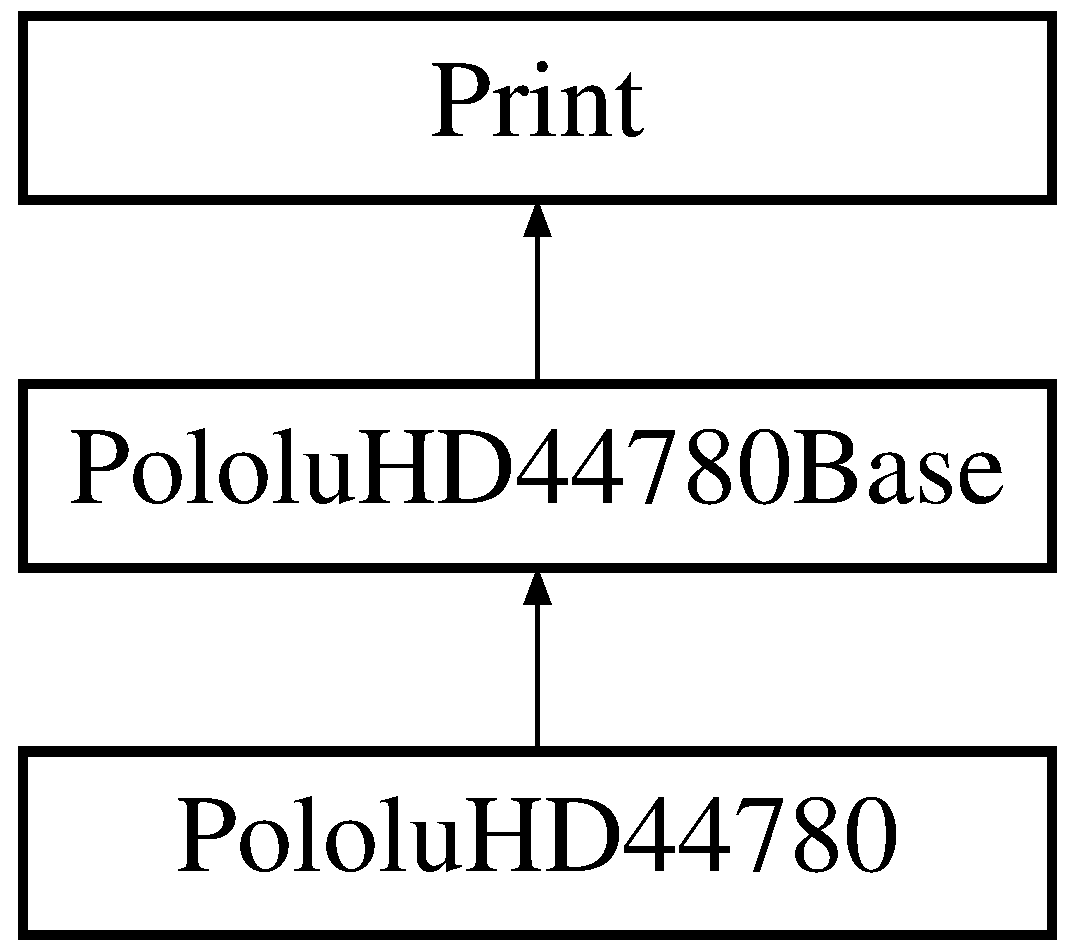
\includegraphics[height=3.000000cm]{class_pololu_h_d44780}
\end{center}
\end{figure}
\doxysubsection*{Public Member Functions}
\begin{DoxyCompactItemize}
\item 
\mbox{\hyperlink{class_pololu_h_d44780_aa435495f74686245db4f89a4d434b3ee}{Pololu\+HD44780}} (uint8\+\_\+t rs, uint8\+\_\+t e, uint8\+\_\+t db4, uint8\+\_\+t db5, uint8\+\_\+t db6, uint8\+\_\+t db7)
\item 
virtual void \mbox{\hyperlink{class_pololu_h_d44780_a876723b26f2dc081bf7f29019079489b}{init\+Pins}} ()
\item 
virtual void \mbox{\hyperlink{class_pololu_h_d44780_a8da2db526de9f1e2314cb02c3ba6121a}{send}} (uint8\+\_\+t data, bool rs\+Value, bool only4bits)
\item 
void \mbox{\hyperlink{class_pololu_h_d44780_base_a1c2a3edc8cfecde7e6fd2a83c17c0e23}{init}} ()
\item 
void \mbox{\hyperlink{class_pololu_h_d44780_base_a10c1c42406708172fc38b718790ba881}{reinitialize}} ()
\item 
void \mbox{\hyperlink{class_pololu_h_d44780_base_a4d35e9a47ceef1a7582e180165e0eae1}{clear}} ()
\item 
void \mbox{\hyperlink{class_pololu_h_d44780_base_a73d331af44ec2e624aa0468ce13f64e4}{load\+Custom\+Character}} (const uint8\+\_\+t $\ast$picture, uint8\+\_\+t number)
\item 
void \mbox{\hyperlink{class_pololu_h_d44780_base_a4f22d613433fce0e0c661a237ade9aeb}{load\+Custom\+Character}} (const char $\ast$picture, uint8\+\_\+t number)
\item 
void \mbox{\hyperlink{class_pololu_h_d44780_base_a72674b5466690b49b639ae2ec3e4983f}{load\+Custom\+Character\+From\+Ram}} (const uint8\+\_\+t $\ast$picture, uint8\+\_\+t number)
\item 
void \mbox{\hyperlink{class_pololu_h_d44780_base_afd802cdc57783830acfe2415355d9f09}{create\+Char}} (uint8\+\_\+t number, uint8\+\_\+t picture\mbox{[}$\,$\mbox{]})
\item 
void \mbox{\hyperlink{class_pololu_h_d44780_base_a4886df8c888669cf71675072689ace9b}{goto\+XY}} (uint8\+\_\+t x, uint8\+\_\+t y)
\item 
void \mbox{\hyperlink{class_pololu_h_d44780_base_aeb3377822dc672398a991f06a00312c0}{set\+Cursor}} (uint8\+\_\+t col, uint8\+\_\+t row)
\item 
void \mbox{\hyperlink{class_pololu_h_d44780_base_abc2d4e126017565c2a0cf2aac67870a0}{no\+Display}} ()
\item 
void \mbox{\hyperlink{class_pololu_h_d44780_base_af5dd1e137bfe9310a418924b7483fcdf}{display}} ()
\item 
void \mbox{\hyperlink{class_pololu_h_d44780_base_ab40886cf0b563a1806bc9391d00b032d}{no\+Cursor}} ()
\item 
void \mbox{\hyperlink{class_pololu_h_d44780_base_a4fd53028d74561be579103d674aa8eab}{cursor}} ()
\item 
void \mbox{\hyperlink{class_pololu_h_d44780_base_a301afc921881052b166e11cd45ad9696}{no\+Blink}} ()
\item 
void \mbox{\hyperlink{class_pololu_h_d44780_base_ac6e255adf32d5c70c0163422b1ae8e0c}{blink}} ()
\item 
void \mbox{\hyperlink{class_pololu_h_d44780_base_a6a4d8e79beda9f7c81659a8e13c8c338}{cursor\+Solid}} ()
\item 
void \mbox{\hyperlink{class_pololu_h_d44780_base_a6a53a6cffbb77953b5a2c4ae49e288de}{cursor\+Blinking}} ()
\item 
void \mbox{\hyperlink{class_pololu_h_d44780_base_a1db083d254d251c479a577f29bcdcec8}{hide\+Cursor}} ()
\item 
void \mbox{\hyperlink{class_pololu_h_d44780_base_aada34a47663585f60b70e1d6f936f6d3}{scroll\+Display\+Left}} ()
\item 
void \mbox{\hyperlink{class_pololu_h_d44780_base_a411512707f303af75de3c5aea313bf48}{scroll\+Display\+Right}} ()
\item 
void \mbox{\hyperlink{class_pololu_h_d44780_base_ab2d24add3c6da0328055bceb38a6d42c}{home}} ()
\item 
void \mbox{\hyperlink{class_pololu_h_d44780_base_ada551bdb01681eb57bec325778eb38a6}{left\+To\+Right}} ()
\item 
void \mbox{\hyperlink{class_pololu_h_d44780_base_aa3f8d4ba18feb9aa0f0a2fef3c6c2b37}{right\+To\+Left}} ()
\item 
void \mbox{\hyperlink{class_pololu_h_d44780_base_ad5104d9651fd95704d1ae192073b0d61}{autoscroll}} ()
\item 
void \mbox{\hyperlink{class_pololu_h_d44780_base_aee80e23d270913dd2c353e7bd5408249}{no\+Autoscroll}} ()
\item 
void \mbox{\hyperlink{class_pololu_h_d44780_base_a449ad8d9ff7afb90667da0003a39af3b}{command}} (uint8\+\_\+t cmd)
\item 
virtual size\+\_\+t \mbox{\hyperlink{class_pololu_h_d44780_base_a1aad3b3ce5820dc910174b3c91a5d65e}{write}} (uint8\+\_\+t c)
\item 
virtual size\+\_\+t \mbox{\hyperlink{class_pololu_h_d44780_base_a965028ffd2313e9eaa968348effcab81}{write}} (const uint8\+\_\+t $\ast$buffer, size\+\_\+t size)
\end{DoxyCompactItemize}


\doxysubsection{Detailed Description}
Main class for interfacing with the HD44780 LCDs. 

This class is suitable for controlling an HD44780 LCD assuming that the LCD\textquotesingle{}s RS, E, DB4, DB5, DB6, and DB7 pins are each connected to a pin on the microcontroller, each of those six microcontroller pins is supported by the Arduino\textquotesingle{}s {\ttfamily pin\+Mode} and {\ttfamily digital\+Write} functions, and those pins are not being used for any other purpose that conflicts with the LCD.

This class sets the E pin to be an output driving low the first time you use the LCD, and it assumes that no other code will change that pin. You cannot use E for any other purposes because if the LCD sees a pulse on the E pin then it might consider that to be a command or data, and the LCD state will become corrupted.

For the other pins (RS, DB4, DB5, and DB6), this library reconfigures them each time they are used, so it is OK if you have other code that uses those pins for other purposes. Before writing to the LCD, you just need to disable any peripherals (such as UARTs) that override the output values of those pins.

If you cannot meet these conditions, you might be able to control your LCD using a custom subclass of \mbox{\hyperlink{class_pololu_h_d44780_base}{Pololu\+HD44780\+Base}}. You can use this class as a reference for how to do that. 

Definition at line \mbox{\hyperlink{_pololu_h_d44780_8h_source_l00360}{360}} of file \mbox{\hyperlink{_pololu_h_d44780_8h_source}{Pololu\+HD44780.\+h}}.



\doxysubsection{Constructor \& Destructor Documentation}
\mbox{\Hypertarget{class_pololu_h_d44780_aa435495f74686245db4f89a4d434b3ee}\label{class_pololu_h_d44780_aa435495f74686245db4f89a4d434b3ee}} 
\index{PololuHD44780@{PololuHD44780}!PololuHD44780@{PololuHD44780}}
\index{PololuHD44780@{PololuHD44780}!PololuHD44780@{PololuHD44780}}
\doxysubsubsection{\texorpdfstring{PololuHD44780()}{PololuHD44780()}}
{\footnotesize\ttfamily Pololu\+HD44780\+::\+Pololu\+HD44780 (\begin{DoxyParamCaption}\item[{uint8\+\_\+t}]{rs,  }\item[{uint8\+\_\+t}]{e,  }\item[{uint8\+\_\+t}]{db4,  }\item[{uint8\+\_\+t}]{db5,  }\item[{uint8\+\_\+t}]{db6,  }\item[{uint8\+\_\+t}]{db7 }\end{DoxyParamCaption})\hspace{0.3cm}{\ttfamily [inline]}}

Creates a new instance of \mbox{\hyperlink{class_pololu_h_d44780}{Pololu\+HD44780}}.


\begin{DoxyParams}{Parameters}
{\em rs} & The pin number for the microcontroller pin that is connected to the RS pin of the LCD. \\
\hline
{\em e} & The pin number for the microcontroller pin that is connected to the E pin of the LCD. \\
\hline
{\em db4} & The pin number for the microcontroller pin that is connected to the DB4 pin of the LCD. \\
\hline
{\em db5} & The pin number for the microcontroller pin that is connected to the DB5 pin of the LCD. \\
\hline
{\em db6} & The pin number for the microcontroller pin that is connected to the DB6 pin of the LCD. \\
\hline
{\em db7} & The pin number for the microcontroller pin that is connected to the DB7 pin of the LCD. \\
\hline
\end{DoxyParams}


Definition at line \mbox{\hyperlink{_pololu_h_d44780_8h_source_l00378}{378}} of file \mbox{\hyperlink{_pololu_h_d44780_8h_source}{Pololu\+HD44780.\+h}}.



\doxysubsection{Member Function Documentation}
\mbox{\Hypertarget{class_pololu_h_d44780_base_ad5104d9651fd95704d1ae192073b0d61}\label{class_pololu_h_d44780_base_ad5104d9651fd95704d1ae192073b0d61}} 
\index{PololuHD44780@{PololuHD44780}!autoscroll@{autoscroll}}
\index{autoscroll@{autoscroll}!PololuHD44780@{PololuHD44780}}
\doxysubsubsection{\texorpdfstring{autoscroll()}{autoscroll()}}
{\footnotesize\ttfamily void Pololu\+HD44780\+Base\+::autoscroll (\begin{DoxyParamCaption}{ }\end{DoxyParamCaption})\hspace{0.3cm}{\ttfamily [inherited]}}

Turns on auto-\/scrolling.

When auto-\/scrolling is enabled, every time a character is written, the screen will automatically scroll by one column in the appropriate direction. 

Definition at line \mbox{\hyperlink{_pololu_h_d44780_8cpp_source_l00214}{214}} of file \mbox{\hyperlink{_pololu_h_d44780_8cpp_source}{Pololu\+HD44780.\+cpp}}.

\mbox{\Hypertarget{class_pololu_h_d44780_base_ac6e255adf32d5c70c0163422b1ae8e0c}\label{class_pololu_h_d44780_base_ac6e255adf32d5c70c0163422b1ae8e0c}} 
\index{PololuHD44780@{PololuHD44780}!blink@{blink}}
\index{blink@{blink}!PololuHD44780@{PololuHD44780}}
\doxysubsubsection{\texorpdfstring{blink()}{blink()}}
{\footnotesize\ttfamily void Pololu\+HD44780\+Base\+::blink (\begin{DoxyParamCaption}{ }\end{DoxyParamCaption})\hspace{0.3cm}{\ttfamily [inherited]}}

Shows the blinking cursor.

This function sets the LCD\textquotesingle{}s \char`\"{}\+B\char`\"{} configuration bit without changing the other bits.

The cursor will normally be a blinking rectangle, but there could also be a row of solid black pixels at the bottom if previous commands have enabled the solid cursor. For this reason, it is usually better to call \mbox{\hyperlink{class_pololu_h_d44780_base_a6a4d8e79beda9f7c81659a8e13c8c338}{cursor\+Solid()}} or \mbox{\hyperlink{class_pololu_h_d44780_base_a6a53a6cffbb77953b5a2c4ae49e288de}{cursor\+Blinking()}} instead. This function is only provided for compatibilty with the Liquid\+Crystal library. 

Definition at line \mbox{\hyperlink{_pololu_h_d44780_8cpp_source_l00177}{177}} of file \mbox{\hyperlink{_pololu_h_d44780_8cpp_source}{Pololu\+HD44780.\+cpp}}.

\mbox{\Hypertarget{class_pololu_h_d44780_base_a4d35e9a47ceef1a7582e180165e0eae1}\label{class_pololu_h_d44780_base_a4d35e9a47ceef1a7582e180165e0eae1}} 
\index{PololuHD44780@{PololuHD44780}!clear@{clear}}
\index{clear@{clear}!PololuHD44780@{PololuHD44780}}
\doxysubsubsection{\texorpdfstring{clear()}{clear()}}
{\footnotesize\ttfamily void Pololu\+HD44780\+Base\+::clear (\begin{DoxyParamCaption}{ }\end{DoxyParamCaption})\hspace{0.3cm}{\ttfamily [inherited]}}

Clear the contents of the LCDs, resets the cursor position to the upper left, and resets the scroll position. 

Definition at line \mbox{\hyperlink{_pololu_h_d44780_8cpp_source_l00078}{78}} of file \mbox{\hyperlink{_pololu_h_d44780_8cpp_source}{Pololu\+HD44780.\+cpp}}.

\mbox{\Hypertarget{class_pololu_h_d44780_base_a449ad8d9ff7afb90667da0003a39af3b}\label{class_pololu_h_d44780_base_a449ad8d9ff7afb90667da0003a39af3b}} 
\index{PololuHD44780@{PololuHD44780}!command@{command}}
\index{command@{command}!PololuHD44780@{PololuHD44780}}
\doxysubsubsection{\texorpdfstring{command()}{command()}}
{\footnotesize\ttfamily void Pololu\+HD44780\+Base\+::command (\begin{DoxyParamCaption}\item[{uint8\+\_\+t}]{cmd }\end{DoxyParamCaption})\hspace{0.3cm}{\ttfamily [inline]}, {\ttfamily [inherited]}}

Send an arbitrary command to the LCD. This is here for compatibility with the Liquid\+Crystal library. 

Definition at line \mbox{\hyperlink{_pololu_h_d44780_8h_source_l00294}{294}} of file \mbox{\hyperlink{_pololu_h_d44780_8h_source}{Pololu\+HD44780.\+h}}.

\mbox{\Hypertarget{class_pololu_h_d44780_base_afd802cdc57783830acfe2415355d9f09}\label{class_pololu_h_d44780_base_afd802cdc57783830acfe2415355d9f09}} 
\index{PololuHD44780@{PololuHD44780}!createChar@{createChar}}
\index{createChar@{createChar}!PololuHD44780@{PololuHD44780}}
\doxysubsubsection{\texorpdfstring{createChar()}{createChar()}}
{\footnotesize\ttfamily void Pololu\+HD44780\+Base\+::create\+Char (\begin{DoxyParamCaption}\item[{uint8\+\_\+t}]{number,  }\item[{uint8\+\_\+t}]{picture\mbox{[}$\,$\mbox{]} }\end{DoxyParamCaption})\hspace{0.3cm}{\ttfamily [inline]}, {\ttfamily [inherited]}}

Defines a custom character. This is provided for compatibility with the Liquid\+Crystal library. 

Definition at line \mbox{\hyperlink{_pololu_h_d44780_8h_source_l00152}{152}} of file \mbox{\hyperlink{_pololu_h_d44780_8h_source}{Pololu\+HD44780.\+h}}.

\mbox{\Hypertarget{class_pololu_h_d44780_base_a4fd53028d74561be579103d674aa8eab}\label{class_pololu_h_d44780_base_a4fd53028d74561be579103d674aa8eab}} 
\index{PololuHD44780@{PololuHD44780}!cursor@{cursor}}
\index{cursor@{cursor}!PololuHD44780@{PololuHD44780}}
\doxysubsubsection{\texorpdfstring{cursor()}{cursor()}}
{\footnotesize\ttfamily void Pololu\+HD44780\+Base\+::cursor (\begin{DoxyParamCaption}{ }\end{DoxyParamCaption})\hspace{0.3cm}{\ttfamily [inherited]}}

Shows the solid cursor.

This function sets the LCD\textquotesingle{}s \char`\"{}\+C\char`\"{} configuration bit without changing the other bits.

The cursor will normally be a solid line in the bottom row, but there could be a blinking rectangle superimposed on it if previous commands have enabled the blinking cursor. For this reason, it is usually better to call \mbox{\hyperlink{class_pololu_h_d44780_base_a6a4d8e79beda9f7c81659a8e13c8c338}{cursor\+Solid()}} or \mbox{\hyperlink{class_pololu_h_d44780_base_a6a53a6cffbb77953b5a2c4ae49e288de}{cursor\+Blinking()}} instead. This function is only provided for compatibility with the Liquid\+Crystal library. 

Definition at line \mbox{\hyperlink{_pololu_h_d44780_8cpp_source_l00167}{167}} of file \mbox{\hyperlink{_pololu_h_d44780_8cpp_source}{Pololu\+HD44780.\+cpp}}.

\mbox{\Hypertarget{class_pololu_h_d44780_base_a6a53a6cffbb77953b5a2c4ae49e288de}\label{class_pololu_h_d44780_base_a6a53a6cffbb77953b5a2c4ae49e288de}} 
\index{PololuHD44780@{PololuHD44780}!cursorBlinking@{cursorBlinking}}
\index{cursorBlinking@{cursorBlinking}!PololuHD44780@{PololuHD44780}}
\doxysubsubsection{\texorpdfstring{cursorBlinking()}{cursorBlinking()}}
{\footnotesize\ttfamily void Pololu\+HD44780\+Base\+::cursor\+Blinking (\begin{DoxyParamCaption}{ }\end{DoxyParamCaption})\hspace{0.3cm}{\ttfamily [inherited]}}

Enables a cursor that appears as a blinking black rectangle.

This sets the LCD\textquotesingle{}s \char`\"{}\+C\char`\"{} and \char`\"{}\+B\char`\"{} configuration bits.

Note that the cursor will not be shown if the display is currently off (due to a call to \mbox{\hyperlink{class_pololu_h_d44780_base_abc2d4e126017565c2a0cf2aac67870a0}{no\+Display()}}), or if the cursor position is not within the bounds of the screen. 

Definition at line \mbox{\hyperlink{_pololu_h_d44780_8cpp_source_l00142}{142}} of file \mbox{\hyperlink{_pololu_h_d44780_8cpp_source}{Pololu\+HD44780.\+cpp}}.

\mbox{\Hypertarget{class_pololu_h_d44780_base_a6a4d8e79beda9f7c81659a8e13c8c338}\label{class_pololu_h_d44780_base_a6a4d8e79beda9f7c81659a8e13c8c338}} 
\index{PololuHD44780@{PololuHD44780}!cursorSolid@{cursorSolid}}
\index{cursorSolid@{cursorSolid}!PololuHD44780@{PololuHD44780}}
\doxysubsubsection{\texorpdfstring{cursorSolid()}{cursorSolid()}}
{\footnotesize\ttfamily void Pololu\+HD44780\+Base\+::cursor\+Solid (\begin{DoxyParamCaption}{ }\end{DoxyParamCaption})\hspace{0.3cm}{\ttfamily [inherited]}}

Enables a cursor that appears as a solid line in the bottom row.

This sets the LCD\textquotesingle{}s \char`\"{}\+C\char`\"{} configuration bit and clears its \char`\"{}\+B\char`\"{} bit.

Note that the cursor will not be shown if the display is currently off (due to a call to \mbox{\hyperlink{class_pololu_h_d44780_base_abc2d4e126017565c2a0cf2aac67870a0}{no\+Display()}}), or if the cursor position is not within the bounds of the screen. 

Definition at line \mbox{\hyperlink{_pololu_h_d44780_8cpp_source_l00137}{137}} of file \mbox{\hyperlink{_pololu_h_d44780_8cpp_source}{Pololu\+HD44780.\+cpp}}.

\mbox{\Hypertarget{class_pololu_h_d44780_base_af5dd1e137bfe9310a418924b7483fcdf}\label{class_pololu_h_d44780_base_af5dd1e137bfe9310a418924b7483fcdf}} 
\index{PololuHD44780@{PololuHD44780}!display@{display}}
\index{display@{display}!PololuHD44780@{PololuHD44780}}
\doxysubsubsection{\texorpdfstring{display()}{display()}}
{\footnotesize\ttfamily void Pololu\+HD44780\+Base\+::display (\begin{DoxyParamCaption}{ }\end{DoxyParamCaption})\hspace{0.3cm}{\ttfamily [inherited]}}

Turns the display on. This should only be needed if \mbox{\hyperlink{class_pololu_h_d44780_base_abc2d4e126017565c2a0cf2aac67870a0}{no\+Display()}} was previously called. 

Definition at line \mbox{\hyperlink{_pololu_h_d44780_8cpp_source_l00157}{157}} of file \mbox{\hyperlink{_pololu_h_d44780_8cpp_source}{Pololu\+HD44780.\+cpp}}.

\mbox{\Hypertarget{class_pololu_h_d44780_base_a4886df8c888669cf71675072689ace9b}\label{class_pololu_h_d44780_base_a4886df8c888669cf71675072689ace9b}} 
\index{PololuHD44780@{PololuHD44780}!gotoXY@{gotoXY}}
\index{gotoXY@{gotoXY}!PololuHD44780@{PololuHD44780}}
\doxysubsubsection{\texorpdfstring{gotoXY()}{gotoXY()}}
{\footnotesize\ttfamily void Pololu\+HD44780\+Base\+::goto\+XY (\begin{DoxyParamCaption}\item[{uint8\+\_\+t}]{x,  }\item[{uint8\+\_\+t}]{y }\end{DoxyParamCaption})\hspace{0.3cm}{\ttfamily [inherited]}}

Change the location of the cursor. The cursor (whether visible or invisible), is the place where the next character written to the LCD will be displayed.

Note that the scrolling features of the LCD change the correspondence between the {\ttfamily x} parameter and the physical column that the data is displayed on. See the \char`\"{}\+LCD scrolling\char`\"{} section above for more information.


\begin{DoxyParams}{Parameters}
{\em x} & The number of the column to go to, with 0 being the leftmost column. \\
\hline
{\em y} & The number of the row to go to, with 0 being the top row. \\
\hline
\end{DoxyParams}


Definition at line \mbox{\hyperlink{_pololu_h_d44780_8cpp_source_l00088}{88}} of file \mbox{\hyperlink{_pololu_h_d44780_8cpp_source}{Pololu\+HD44780.\+cpp}}.

\mbox{\Hypertarget{class_pololu_h_d44780_base_a1db083d254d251c479a577f29bcdcec8}\label{class_pololu_h_d44780_base_a1db083d254d251c479a577f29bcdcec8}} 
\index{PololuHD44780@{PololuHD44780}!hideCursor@{hideCursor}}
\index{hideCursor@{hideCursor}!PololuHD44780@{PololuHD44780}}
\doxysubsubsection{\texorpdfstring{hideCursor()}{hideCursor()}}
{\footnotesize\ttfamily void Pololu\+HD44780\+Base\+::hide\+Cursor (\begin{DoxyParamCaption}{ }\end{DoxyParamCaption})\hspace{0.3cm}{\ttfamily [inherited]}}

Hides the solid and blinking cursors.

This clears the LCD\textquotesingle{}s \char`\"{}\+C\char`\"{} and \char`\"{}\+B\char`\"{} configuration bits. 

Definition at line \mbox{\hyperlink{_pololu_h_d44780_8cpp_source_l00147}{147}} of file \mbox{\hyperlink{_pololu_h_d44780_8cpp_source}{Pololu\+HD44780.\+cpp}}.

\mbox{\Hypertarget{class_pololu_h_d44780_base_ab2d24add3c6da0328055bceb38a6d42c}\label{class_pololu_h_d44780_base_ab2d24add3c6da0328055bceb38a6d42c}} 
\index{PololuHD44780@{PololuHD44780}!home@{home}}
\index{home@{home}!PololuHD44780@{PololuHD44780}}
\doxysubsubsection{\texorpdfstring{home()}{home()}}
{\footnotesize\ttfamily void Pololu\+HD44780\+Base\+::home (\begin{DoxyParamCaption}{ }\end{DoxyParamCaption})\hspace{0.3cm}{\ttfamily [inherited]}}

Resets the screen scrolling position back to the default and moves the cursor to the upper left corner of the screen.

This command takes about 1600 microseconds, so it would be faster to instead call \mbox{\hyperlink{class_pololu_h_d44780_base_aada34a47663585f60b70e1d6f936f6d3}{scroll\+Display\+Left()}} or \mbox{\hyperlink{class_pololu_h_d44780_base_a411512707f303af75de3c5aea313bf48}{scroll\+Display\+Right()}} the appropriate number of times and then call goto\+XY(0, 0). 

Definition at line \mbox{\hyperlink{_pololu_h_d44780_8cpp_source_l00192}{192}} of file \mbox{\hyperlink{_pololu_h_d44780_8cpp_source}{Pololu\+HD44780.\+cpp}}.

\mbox{\Hypertarget{class_pololu_h_d44780_base_a1c2a3edc8cfecde7e6fd2a83c17c0e23}\label{class_pololu_h_d44780_base_a1c2a3edc8cfecde7e6fd2a83c17c0e23}} 
\index{PololuHD44780@{PololuHD44780}!init@{init}}
\index{init@{init}!PololuHD44780@{PololuHD44780}}
\doxysubsubsection{\texorpdfstring{init()}{init()}}
{\footnotesize\ttfamily void Pololu\+HD44780\+Base\+::init (\begin{DoxyParamCaption}{ }\end{DoxyParamCaption})\hspace{0.3cm}{\ttfamily [inline]}, {\ttfamily [inherited]}}

Initialize the LCD if it has not already been initialized. 

Definition at line \mbox{\hyperlink{_pololu_h_d44780_8h_source_l00067}{67}} of file \mbox{\hyperlink{_pololu_h_d44780_8h_source}{Pololu\+HD44780.\+h}}.

\mbox{\Hypertarget{class_pololu_h_d44780_a876723b26f2dc081bf7f29019079489b}\label{class_pololu_h_d44780_a876723b26f2dc081bf7f29019079489b}} 
\index{PololuHD44780@{PololuHD44780}!initPins@{initPins}}
\index{initPins@{initPins}!PololuHD44780@{PololuHD44780}}
\doxysubsubsection{\texorpdfstring{initPins()}{initPins()}}
{\footnotesize\ttfamily virtual void Pololu\+HD44780\+::init\+Pins (\begin{DoxyParamCaption}{ }\end{DoxyParamCaption})\hspace{0.3cm}{\ttfamily [inline]}, {\ttfamily [virtual]}}

Initializes the pins so that the \mbox{\hyperlink{class_pololu_h_d44780_a8da2db526de9f1e2314cb02c3ba6121a}{send()}} function can be called successfully. This is the first step of initializing the LCD. 

Implements \mbox{\hyperlink{class_pololu_h_d44780_base_a9c2a2e0dfb089a6c21aa12a6a5299750}{Pololu\+HD44780\+Base}}.



Definition at line \mbox{\hyperlink{_pololu_h_d44780_8h_source_l00389}{389}} of file \mbox{\hyperlink{_pololu_h_d44780_8h_source}{Pololu\+HD44780.\+h}}.

\mbox{\Hypertarget{class_pololu_h_d44780_base_ada551bdb01681eb57bec325778eb38a6}\label{class_pololu_h_d44780_base_ada551bdb01681eb57bec325778eb38a6}} 
\index{PololuHD44780@{PololuHD44780}!leftToRight@{leftToRight}}
\index{leftToRight@{leftToRight}!PololuHD44780@{PololuHD44780}}
\doxysubsubsection{\texorpdfstring{leftToRight()}{leftToRight()}}
{\footnotesize\ttfamily void Pololu\+HD44780\+Base\+::left\+To\+Right (\begin{DoxyParamCaption}{ }\end{DoxyParamCaption})\hspace{0.3cm}{\ttfamily [inherited]}}

Puts the LCD into left-\/to-\/right mode\+: the cursor will shift to the right after any character is written. This is the default behavior. 

Definition at line \mbox{\hyperlink{_pololu_h_d44780_8cpp_source_l00204}{204}} of file \mbox{\hyperlink{_pololu_h_d44780_8cpp_source}{Pololu\+HD44780.\+cpp}}.

\mbox{\Hypertarget{class_pololu_h_d44780_base_a4f22d613433fce0e0c661a237ade9aeb}\label{class_pololu_h_d44780_base_a4f22d613433fce0e0c661a237ade9aeb}} 
\index{PololuHD44780@{PololuHD44780}!loadCustomCharacter@{loadCustomCharacter}}
\index{loadCustomCharacter@{loadCustomCharacter}!PololuHD44780@{PololuHD44780}}
\doxysubsubsection{\texorpdfstring{loadCustomCharacter()}{loadCustomCharacter()}\hspace{0.1cm}{\footnotesize\ttfamily [1/2]}}
{\footnotesize\ttfamily void Pololu\+HD44780\+Base\+::load\+Custom\+Character (\begin{DoxyParamCaption}\item[{const char $\ast$}]{picture,  }\item[{uint8\+\_\+t}]{number }\end{DoxyParamCaption})\hspace{0.3cm}{\ttfamily [inline]}, {\ttfamily [inherited]}}

This overload of load\+Custom\+Character is only provided for compatibility with Orangutan\+LCD; a lot of Orangutan code defines an array of chars for custom character pictures. 

Definition at line \mbox{\hyperlink{_pololu_h_d44780_8h_source_l00145}{145}} of file \mbox{\hyperlink{_pololu_h_d44780_8h_source}{Pololu\+HD44780.\+h}}.

\mbox{\Hypertarget{class_pololu_h_d44780_base_a73d331af44ec2e624aa0468ce13f64e4}\label{class_pololu_h_d44780_base_a73d331af44ec2e624aa0468ce13f64e4}} 
\index{PololuHD44780@{PololuHD44780}!loadCustomCharacter@{loadCustomCharacter}}
\index{loadCustomCharacter@{loadCustomCharacter}!PololuHD44780@{PololuHD44780}}
\doxysubsubsection{\texorpdfstring{loadCustomCharacter()}{loadCustomCharacter()}\hspace{0.1cm}{\footnotesize\ttfamily [2/2]}}
{\footnotesize\ttfamily void Pololu\+HD44780\+Base\+::load\+Custom\+Character (\begin{DoxyParamCaption}\item[{const uint8\+\_\+t $\ast$}]{picture,  }\item[{uint8\+\_\+t}]{number }\end{DoxyParamCaption})\hspace{0.3cm}{\ttfamily [inherited]}}

Defines a custom character. 
\begin{DoxyParams}{Parameters}
{\em picture} & A pointer to the character dot pattern, in program space. \\
\hline
{\em number} & A number between 0 and 7. \\
\hline
\end{DoxyParams}


Definition at line \mbox{\hyperlink{_pololu_h_d44780_8cpp_source_l00103}{103}} of file \mbox{\hyperlink{_pololu_h_d44780_8cpp_source}{Pololu\+HD44780.\+cpp}}.

\mbox{\Hypertarget{class_pololu_h_d44780_base_a72674b5466690b49b639ae2ec3e4983f}\label{class_pololu_h_d44780_base_a72674b5466690b49b639ae2ec3e4983f}} 
\index{PololuHD44780@{PololuHD44780}!loadCustomCharacterFromRam@{loadCustomCharacterFromRam}}
\index{loadCustomCharacterFromRam@{loadCustomCharacterFromRam}!PololuHD44780@{PololuHD44780}}
\doxysubsubsection{\texorpdfstring{loadCustomCharacterFromRam()}{loadCustomCharacterFromRam()}}
{\footnotesize\ttfamily void Pololu\+HD44780\+Base\+::load\+Custom\+Character\+From\+Ram (\begin{DoxyParamCaption}\item[{const uint8\+\_\+t $\ast$}]{picture,  }\item[{uint8\+\_\+t}]{number }\end{DoxyParamCaption})\hspace{0.3cm}{\ttfamily [inherited]}}

Defines a custom character from RAM. 
\begin{DoxyParams}{Parameters}
{\em picture} & A pointer to the character dot pattern, in RAM. \\
\hline
{\em number} & A number between 0 and 7. \\
\hline
\end{DoxyParams}


Definition at line \mbox{\hyperlink{_pololu_h_d44780_8cpp_source_l00117}{117}} of file \mbox{\hyperlink{_pololu_h_d44780_8cpp_source}{Pololu\+HD44780.\+cpp}}.

\mbox{\Hypertarget{class_pololu_h_d44780_base_aee80e23d270913dd2c353e7bd5408249}\label{class_pololu_h_d44780_base_aee80e23d270913dd2c353e7bd5408249}} 
\index{PololuHD44780@{PololuHD44780}!noAutoscroll@{noAutoscroll}}
\index{noAutoscroll@{noAutoscroll}!PololuHD44780@{PololuHD44780}}
\doxysubsubsection{\texorpdfstring{noAutoscroll()}{noAutoscroll()}}
{\footnotesize\ttfamily void Pololu\+HD44780\+Base\+::no\+Autoscroll (\begin{DoxyParamCaption}{ }\end{DoxyParamCaption})\hspace{0.3cm}{\ttfamily [inherited]}}

Turns off auto-\/scrolling. Auto-\/scrolling is off by default. 

Definition at line \mbox{\hyperlink{_pololu_h_d44780_8cpp_source_l00219}{219}} of file \mbox{\hyperlink{_pololu_h_d44780_8cpp_source}{Pololu\+HD44780.\+cpp}}.

\mbox{\Hypertarget{class_pololu_h_d44780_base_a301afc921881052b166e11cd45ad9696}\label{class_pololu_h_d44780_base_a301afc921881052b166e11cd45ad9696}} 
\index{PololuHD44780@{PololuHD44780}!noBlink@{noBlink}}
\index{noBlink@{noBlink}!PololuHD44780@{PololuHD44780}}
\doxysubsubsection{\texorpdfstring{noBlink()}{noBlink()}}
{\footnotesize\ttfamily void Pololu\+HD44780\+Base\+::no\+Blink (\begin{DoxyParamCaption}{ }\end{DoxyParamCaption})\hspace{0.3cm}{\ttfamily [inherited]}}

Hides the blinking cursor.

This functions clears the LCD\textquotesingle{}s \char`\"{}\+B\char`\"{} configuration bit without changing the other bits.

Calling this function does not enable or disable the solid cursor (a solid line in the bottom row) so it is usually better to call \mbox{\hyperlink{class_pololu_h_d44780_base_a1db083d254d251c479a577f29bcdcec8}{hide\+Cursor()}} or \mbox{\hyperlink{class_pololu_h_d44780_base_a6a4d8e79beda9f7c81659a8e13c8c338}{cursor\+Solid()}} instead. This function is only provided for compatibilty with the Liquid\+Crystal library. 

Definition at line \mbox{\hyperlink{_pololu_h_d44780_8cpp_source_l00172}{172}} of file \mbox{\hyperlink{_pololu_h_d44780_8cpp_source}{Pololu\+HD44780.\+cpp}}.

\mbox{\Hypertarget{class_pololu_h_d44780_base_ab40886cf0b563a1806bc9391d00b032d}\label{class_pololu_h_d44780_base_ab40886cf0b563a1806bc9391d00b032d}} 
\index{PololuHD44780@{PololuHD44780}!noCursor@{noCursor}}
\index{noCursor@{noCursor}!PololuHD44780@{PololuHD44780}}
\doxysubsubsection{\texorpdfstring{noCursor()}{noCursor()}}
{\footnotesize\ttfamily void Pololu\+HD44780\+Base\+::no\+Cursor (\begin{DoxyParamCaption}{ }\end{DoxyParamCaption})\hspace{0.3cm}{\ttfamily [inherited]}}

Hides the solid cursor.

This function clears the LCD\textquotesingle{}s \char`\"{}\+C\char`\"{} configuration bit without changing the other bits.

If the \char`\"{}\+B\char`\"{} bit is set to 1, a blinking cursor will still be displayed even after calling this function. For that reason, it is usually better to call \mbox{\hyperlink{class_pololu_h_d44780_base_a1db083d254d251c479a577f29bcdcec8}{hide\+Cursor()}} instead. This function is only provided for compatibility with the Liquid\+Crystal library. 

Definition at line \mbox{\hyperlink{_pololu_h_d44780_8cpp_source_l00162}{162}} of file \mbox{\hyperlink{_pololu_h_d44780_8cpp_source}{Pololu\+HD44780.\+cpp}}.

\mbox{\Hypertarget{class_pololu_h_d44780_base_abc2d4e126017565c2a0cf2aac67870a0}\label{class_pololu_h_d44780_base_abc2d4e126017565c2a0cf2aac67870a0}} 
\index{PololuHD44780@{PololuHD44780}!noDisplay@{noDisplay}}
\index{noDisplay@{noDisplay}!PololuHD44780@{PololuHD44780}}
\doxysubsubsection{\texorpdfstring{noDisplay()}{noDisplay()}}
{\footnotesize\ttfamily void Pololu\+HD44780\+Base\+::no\+Display (\begin{DoxyParamCaption}{ }\end{DoxyParamCaption})\hspace{0.3cm}{\ttfamily [inherited]}}

Turns off the display while preserving its state.

You can turn the display on again by calling \mbox{\hyperlink{class_pololu_h_d44780_base_af5dd1e137bfe9310a418924b7483fcdf}{display()}}. 

Definition at line \mbox{\hyperlink{_pololu_h_d44780_8cpp_source_l00152}{152}} of file \mbox{\hyperlink{_pololu_h_d44780_8cpp_source}{Pololu\+HD44780.\+cpp}}.

\mbox{\Hypertarget{class_pololu_h_d44780_base_a10c1c42406708172fc38b718790ba881}\label{class_pololu_h_d44780_base_a10c1c42406708172fc38b718790ba881}} 
\index{PololuHD44780@{PololuHD44780}!reinitialize@{reinitialize}}
\index{reinitialize@{reinitialize}!PololuHD44780@{PololuHD44780}}
\doxysubsubsection{\texorpdfstring{reinitialize()}{reinitialize()}}
{\footnotesize\ttfamily void Pololu\+HD44780\+Base\+::reinitialize (\begin{DoxyParamCaption}{ }\end{DoxyParamCaption})\hspace{0.3cm}{\ttfamily [inline]}, {\ttfamily [inherited]}}

Reinitialize the LCD. This performs the same initialization that is done automatically the first time any function is called that writes to the LCD. This is useful if you want to get it back to a totally clean state. 

Definition at line \mbox{\hyperlink{_pololu_h_d44780_8h_source_l00080}{80}} of file \mbox{\hyperlink{_pololu_h_d44780_8h_source}{Pololu\+HD44780.\+h}}.

\mbox{\Hypertarget{class_pololu_h_d44780_base_aa3f8d4ba18feb9aa0f0a2fef3c6c2b37}\label{class_pololu_h_d44780_base_aa3f8d4ba18feb9aa0f0a2fef3c6c2b37}} 
\index{PololuHD44780@{PololuHD44780}!rightToLeft@{rightToLeft}}
\index{rightToLeft@{rightToLeft}!PololuHD44780@{PololuHD44780}}
\doxysubsubsection{\texorpdfstring{rightToLeft()}{rightToLeft()}}
{\footnotesize\ttfamily void Pololu\+HD44780\+Base\+::right\+To\+Left (\begin{DoxyParamCaption}{ }\end{DoxyParamCaption})\hspace{0.3cm}{\ttfamily [inherited]}}

Puts the LCD into right-\/to-\/left mode\+: the cursor will shift to the left after any character is written. 

Definition at line \mbox{\hyperlink{_pololu_h_d44780_8cpp_source_l00209}{209}} of file \mbox{\hyperlink{_pololu_h_d44780_8cpp_source}{Pololu\+HD44780.\+cpp}}.

\mbox{\Hypertarget{class_pololu_h_d44780_base_aada34a47663585f60b70e1d6f936f6d3}\label{class_pololu_h_d44780_base_aada34a47663585f60b70e1d6f936f6d3}} 
\index{PololuHD44780@{PololuHD44780}!scrollDisplayLeft@{scrollDisplayLeft}}
\index{scrollDisplayLeft@{scrollDisplayLeft}!PololuHD44780@{PololuHD44780}}
\doxysubsubsection{\texorpdfstring{scrollDisplayLeft()}{scrollDisplayLeft()}}
{\footnotesize\ttfamily void Pololu\+HD44780\+Base\+::scroll\+Display\+Left (\begin{DoxyParamCaption}{ }\end{DoxyParamCaption})\hspace{0.3cm}{\ttfamily [inherited]}}

Scrolls everything on the screen one position to the left.

This command takes about 37 microseconds. 

Definition at line \mbox{\hyperlink{_pololu_h_d44780_8cpp_source_l00182}{182}} of file \mbox{\hyperlink{_pololu_h_d44780_8cpp_source}{Pololu\+HD44780.\+cpp}}.

\mbox{\Hypertarget{class_pololu_h_d44780_base_a411512707f303af75de3c5aea313bf48}\label{class_pololu_h_d44780_base_a411512707f303af75de3c5aea313bf48}} 
\index{PololuHD44780@{PololuHD44780}!scrollDisplayRight@{scrollDisplayRight}}
\index{scrollDisplayRight@{scrollDisplayRight}!PololuHD44780@{PololuHD44780}}
\doxysubsubsection{\texorpdfstring{scrollDisplayRight()}{scrollDisplayRight()}}
{\footnotesize\ttfamily void Pololu\+HD44780\+Base\+::scroll\+Display\+Right (\begin{DoxyParamCaption}{ }\end{DoxyParamCaption})\hspace{0.3cm}{\ttfamily [inherited]}}

Scrolls everything on the screen one position to the right.

This command takes about 37 microseconds. 

Definition at line \mbox{\hyperlink{_pololu_h_d44780_8cpp_source_l00187}{187}} of file \mbox{\hyperlink{_pololu_h_d44780_8cpp_source}{Pololu\+HD44780.\+cpp}}.

\mbox{\Hypertarget{class_pololu_h_d44780_a8da2db526de9f1e2314cb02c3ba6121a}\label{class_pololu_h_d44780_a8da2db526de9f1e2314cb02c3ba6121a}} 
\index{PololuHD44780@{PololuHD44780}!send@{send}}
\index{send@{send}!PololuHD44780@{PololuHD44780}}
\doxysubsubsection{\texorpdfstring{send()}{send()}}
{\footnotesize\ttfamily virtual void Pololu\+HD44780\+::send (\begin{DoxyParamCaption}\item[{uint8\+\_\+t}]{data,  }\item[{bool}]{rs\+Value,  }\item[{bool}]{only4bits }\end{DoxyParamCaption})\hspace{0.3cm}{\ttfamily [inline]}, {\ttfamily [virtual]}}

Sends data or commands to the LCD.

The \mbox{\hyperlink{class_pololu_h_d44780_a876723b26f2dc081bf7f29019079489b}{init\+Pins()}} function will always be called before the first time this function is called. This function does not need to worry about the delays necessary to make sure the previous command has finished; that is taken care of by \mbox{\hyperlink{class_pololu_h_d44780_base}{Pololu\+HD44780\+Base}}.

This function, along with \mbox{\hyperlink{class_pololu_h_d44780_a876723b26f2dc081bf7f29019079489b}{init\+Pins()}}, comprise the hardware abstraction layer for the LCD, and must be defined in a subclass of \mbox{\hyperlink{class_pololu_h_d44780_base}{Pololu\+HD44780\+Base}}. All other functions use these two functions to communicate with the LCD.


\begin{DoxyParams}{Parameters}
{\em data} & The data to send to the LCD. \\
\hline
{\em rs\+Value} & True to drive the RS pin high, false to drive it low. \\
\hline
{\em only4bits} & If true, and the LCD is using a 4-\/bit interface, only sends the lower 4 bits of the data. \\
\hline
\end{DoxyParams}


Implements \mbox{\hyperlink{class_pololu_h_d44780_base_a004d5adb9e7c3cc546c6b0ed427dec7b}{Pololu\+HD44780\+Base}}.



Definition at line \mbox{\hyperlink{_pololu_h_d44780_8h_source_l00395}{395}} of file \mbox{\hyperlink{_pololu_h_d44780_8h_source}{Pololu\+HD44780.\+h}}.

\mbox{\Hypertarget{class_pololu_h_d44780_base_aeb3377822dc672398a991f06a00312c0}\label{class_pololu_h_d44780_base_aeb3377822dc672398a991f06a00312c0}} 
\index{PololuHD44780@{PololuHD44780}!setCursor@{setCursor}}
\index{setCursor@{setCursor}!PololuHD44780@{PololuHD44780}}
\doxysubsubsection{\texorpdfstring{setCursor()}{setCursor()}}
{\footnotesize\ttfamily void Pololu\+HD44780\+Base\+::set\+Cursor (\begin{DoxyParamCaption}\item[{uint8\+\_\+t}]{col,  }\item[{uint8\+\_\+t}]{row }\end{DoxyParamCaption})\hspace{0.3cm}{\ttfamily [inline]}, {\ttfamily [inherited]}}

Changes the location of the cursor. This is just a wrapper around goto\+XY provided for compaitibility with the Liquid\+Crystal library. 

Definition at line \mbox{\hyperlink{_pololu_h_d44780_8h_source_l00170}{170}} of file \mbox{\hyperlink{_pololu_h_d44780_8h_source}{Pololu\+HD44780.\+h}}.

\mbox{\Hypertarget{class_pololu_h_d44780_base_a965028ffd2313e9eaa968348effcab81}\label{class_pololu_h_d44780_base_a965028ffd2313e9eaa968348effcab81}} 
\index{PololuHD44780@{PololuHD44780}!write@{write}}
\index{write@{write}!PololuHD44780@{PololuHD44780}}
\doxysubsubsection{\texorpdfstring{write()}{write()}\hspace{0.1cm}{\footnotesize\ttfamily [1/2]}}
{\footnotesize\ttfamily size\+\_\+t Pololu\+HD44780\+Base\+::write (\begin{DoxyParamCaption}\item[{const uint8\+\_\+t $\ast$}]{buffer,  }\item[{size\+\_\+t}]{size }\end{DoxyParamCaption})\hspace{0.3cm}{\ttfamily [virtual]}, {\ttfamily [inherited]}}

Writes multiple characters to the LCD.


\begin{DoxyParams}{Parameters}
{\em buffer} & Pointer to a string of characters in RAM, not necessarily null-\/terminated. \\
\hline
{\em size} & The number of characters to write to the LCD, excluding any null termination character. \\
\hline
\end{DoxyParams}


Definition at line \mbox{\hyperlink{_pololu_h_d44780_8cpp_source_l00068}{68}} of file \mbox{\hyperlink{_pololu_h_d44780_8cpp_source}{Pololu\+HD44780.\+cpp}}.

\mbox{\Hypertarget{class_pololu_h_d44780_base_a1aad3b3ce5820dc910174b3c91a5d65e}\label{class_pololu_h_d44780_base_a1aad3b3ce5820dc910174b3c91a5d65e}} 
\index{PololuHD44780@{PololuHD44780}!write@{write}}
\index{write@{write}!PololuHD44780@{PololuHD44780}}
\doxysubsubsection{\texorpdfstring{write()}{write()}\hspace{0.1cm}{\footnotesize\ttfamily [2/2]}}
{\footnotesize\ttfamily size\+\_\+t Pololu\+HD44780\+Base\+::write (\begin{DoxyParamCaption}\item[{uint8\+\_\+t}]{c }\end{DoxyParamCaption})\hspace{0.3cm}{\ttfamily [virtual]}, {\ttfamily [inherited]}}

Writes a single character to the LCD. 

Definition at line \mbox{\hyperlink{_pololu_h_d44780_8cpp_source_l00062}{62}} of file \mbox{\hyperlink{_pololu_h_d44780_8cpp_source}{Pololu\+HD44780.\+cpp}}.



The documentation for this class was generated from the following file\+:\begin{DoxyCompactItemize}
\item 
\mbox{\hyperlink{_pololu_h_d44780_8h}{Pololu\+HD44780.\+h}}\end{DoxyCompactItemize}

\hypertarget{class_pololu_h_d44780_base}{}\section{Pololu\+H\+D44780\+Base Class Reference}
\label{class_pololu_h_d44780_base}\index{Pololu\+H\+D44780\+Base@{Pololu\+H\+D44780\+Base}}


General class for handling the H\+D44780 protocol.  




{\ttfamily \#include $<$Pololu\+H\+D44780.\+h$>$}

Inheritance diagram for Pololu\+H\+D44780\+Base\+:\begin{figure}[H]
\begin{center}
\leavevmode
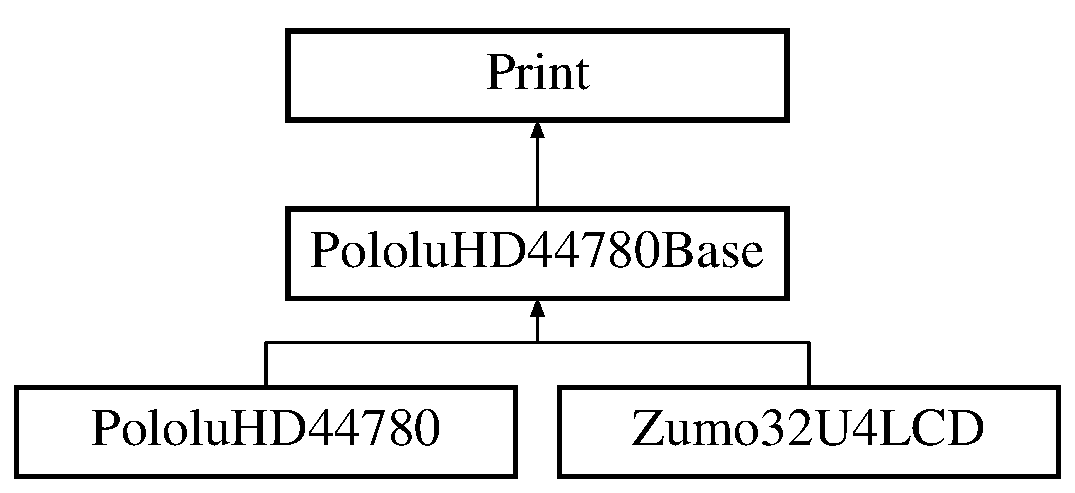
\includegraphics[height=3.000000cm]{class_pololu_h_d44780_base}
\end{center}
\end{figure}
\subsection*{Public Member Functions}
\begin{DoxyCompactItemize}
\item 
virtual void \hyperlink{class_pololu_h_d44780_base_a9c2a2e0dfb089a6c21aa12a6a5299750}{init\+Pins} ()=0
\item 
void \hyperlink{class_pololu_h_d44780_base_a1c2a3edc8cfecde7e6fd2a83c17c0e23}{init} ()
\item 
void \hyperlink{class_pololu_h_d44780_base_a10c1c42406708172fc38b718790ba881}{reinitialize} ()
\item 
virtual void \hyperlink{class_pololu_h_d44780_base_a004d5adb9e7c3cc546c6b0ed427dec7b}{send} (uint8\+\_\+t data, bool rs\+Value, bool only4bits)=0
\item 
void \hyperlink{class_pololu_h_d44780_base_a4d35e9a47ceef1a7582e180165e0eae1}{clear} ()
\item 
void \hyperlink{class_pololu_h_d44780_base_a73d331af44ec2e624aa0468ce13f64e4}{load\+Custom\+Character} (const uint8\+\_\+t $\ast$picture, uint8\+\_\+t number)
\item 
void \hyperlink{class_pololu_h_d44780_base_a72674b5466690b49b639ae2ec3e4983f}{load\+Custom\+Character\+From\+Ram} (const uint8\+\_\+t $\ast$picture, uint8\+\_\+t number)
\item 
void \hyperlink{class_pololu_h_d44780_base_a4f22d613433fce0e0c661a237ade9aeb}{load\+Custom\+Character} (const char $\ast$picture, uint8\+\_\+t number)
\item 
void \hyperlink{class_pololu_h_d44780_base_afd802cdc57783830acfe2415355d9f09}{create\+Char} (uint8\+\_\+t number, uint8\+\_\+t picture\mbox{[}$\,$\mbox{]})
\item 
void \hyperlink{class_pololu_h_d44780_base_a4886df8c888669cf71675072689ace9b}{goto\+XY} (uint8\+\_\+t x, uint8\+\_\+t y)
\item 
void \hyperlink{class_pololu_h_d44780_base_aeb3377822dc672398a991f06a00312c0}{set\+Cursor} (uint8\+\_\+t col, uint8\+\_\+t row)
\item 
void \hyperlink{class_pololu_h_d44780_base_abc2d4e126017565c2a0cf2aac67870a0}{no\+Display} ()
\item 
void \hyperlink{class_pololu_h_d44780_base_af5dd1e137bfe9310a418924b7483fcdf}{display} ()
\item 
void \hyperlink{class_pololu_h_d44780_base_ab40886cf0b563a1806bc9391d00b032d}{no\+Cursor} ()
\item 
void \hyperlink{class_pololu_h_d44780_base_a4fd53028d74561be579103d674aa8eab}{cursor} ()
\item 
void \hyperlink{class_pololu_h_d44780_base_a301afc921881052b166e11cd45ad9696}{no\+Blink} ()
\item 
void \hyperlink{class_pololu_h_d44780_base_ac6e255adf32d5c70c0163422b1ae8e0c}{blink} ()
\item 
void \hyperlink{class_pololu_h_d44780_base_a6a4d8e79beda9f7c81659a8e13c8c338}{cursor\+Solid} ()
\item 
void \hyperlink{class_pololu_h_d44780_base_a6a53a6cffbb77953b5a2c4ae49e288de}{cursor\+Blinking} ()
\item 
void \hyperlink{class_pololu_h_d44780_base_a1db083d254d251c479a577f29bcdcec8}{hide\+Cursor} ()
\item 
void \hyperlink{class_pololu_h_d44780_base_aada34a47663585f60b70e1d6f936f6d3}{scroll\+Display\+Left} ()
\item 
void \hyperlink{class_pololu_h_d44780_base_a411512707f303af75de3c5aea313bf48}{scroll\+Display\+Right} ()
\item 
void \hyperlink{class_pololu_h_d44780_base_ab2d24add3c6da0328055bceb38a6d42c}{home} ()
\item 
void \hyperlink{class_pololu_h_d44780_base_ada551bdb01681eb57bec325778eb38a6}{left\+To\+Right} ()
\item 
void \hyperlink{class_pololu_h_d44780_base_aa3f8d4ba18feb9aa0f0a2fef3c6c2b37}{right\+To\+Left} ()
\item 
void \hyperlink{class_pololu_h_d44780_base_ad5104d9651fd95704d1ae192073b0d61}{autoscroll} ()
\item 
void \hyperlink{class_pololu_h_d44780_base_aee80e23d270913dd2c353e7bd5408249}{no\+Autoscroll} ()
\item 
void \hyperlink{class_pololu_h_d44780_base_a449ad8d9ff7afb90667da0003a39af3b}{command} (uint8\+\_\+t cmd)
\item 
virtual size\+\_\+t \hyperlink{class_pololu_h_d44780_base_a1aad3b3ce5820dc910174b3c91a5d65e}{write} (uint8\+\_\+t c)
\item 
virtual size\+\_\+t \hyperlink{class_pololu_h_d44780_base_a965028ffd2313e9eaa968348effcab81}{write} (const uint8\+\_\+t $\ast$buffer, size\+\_\+t size)
\end{DoxyCompactItemize}


\subsection{Detailed Description}
General class for handling the H\+D44780 protocol. 

This is an abstract class that knows about the H\+D44780 L\+CD commands but does not directly read or write from the actual L\+CD. To make a usable class, you need to define a subclass of \hyperlink{class_pololu_h_d44780_base}{Pololu\+H\+D44780\+Base} and implement the \hyperlink{class_pololu_h_d44780_base_a9c2a2e0dfb089a6c21aa12a6a5299750}{init\+Pins()} and \hyperlink{class_pololu_h_d44780_base_a004d5adb9e7c3cc546c6b0ed427dec7b}{send()} functions.

The subclass will inherit all the functions from \hyperlink{class_pololu_h_d44780_base}{Pololu\+H\+D44780\+Base} which are documented here. It will also inherit all of the functions from the Arduino {\ttfamily Print} class. For more information about what the {\ttfamily Print} class provides, see the \href{http://arduino.cc/en/Serial/Print}{\tt Arduino print() documentation} or look at \href{https://github.com/arduino/Arduino/blob/master/hardware/arduino/cores/arduino/Print.h}{\tt Print.\+h in the Arduino I\+DE source code}.

Most users of this library will not need to directly use this class and should use \hyperlink{class_pololu_h_d44780}{Pololu\+H\+D44780} or some other subclass of \hyperlink{class_pololu_h_d44780_base}{Pololu\+H\+D44780\+Base} defined in a different library.

The \hyperlink{class_pololu_h_d44780_base}{Pololu\+H\+D44780\+Base} class provides several functions related to scrolling\+:


\begin{DoxyItemize}
\item \hyperlink{class_pololu_h_d44780_base_aada34a47663585f60b70e1d6f936f6d3}{scroll\+Display\+Left()} scrolls everything on the screen one position to the left.
\item \hyperlink{class_pololu_h_d44780_base_a411512707f303af75de3c5aea313bf48}{scroll\+Display\+Right()} scrolls everything on the screen one position to the right.
\item \hyperlink{class_pololu_h_d44780_base_ad5104d9651fd95704d1ae192073b0d61}{autoscroll()} and \hyperlink{class_pololu_h_d44780_base_aee80e23d270913dd2c353e7bd5408249}{no\+Autoscroll()} control whether auto-\/scrolling is enabled.
\item \hyperlink{class_pololu_h_d44780_base_ab2d24add3c6da0328055bceb38a6d42c}{home()} and \hyperlink{class_pololu_h_d44780_base_a4d35e9a47ceef1a7582e180165e0eae1}{clear()} both reset the scroll position
\end{DoxyItemize}

The H\+D44780 actually stores 40 columns internally. By default, the left-\/most internal columns are the ones that are actually displayed on the screen, but the scrolling features allow that correspondence to change. The scrolling wraps around, so it is possible to display some of the right-\/most columns on the screen at the same time as some of the left-\/most columns.

For the \hyperlink{class_pololu_h_d44780_base_a4886df8c888669cf71675072689ace9b}{goto\+X\+Y()} function, the x coordinate actually corresponds to the internal column index. The left-\/most internal column has an x coordinate of 0, and the right-\/most has an x coordinate of 39.

For example, if you are controlling a 2{$\times$}8 character L\+CD and you call \hyperlink{class_pololu_h_d44780_base_aada34a47663585f60b70e1d6f936f6d3}{scroll\+Display\+Left()} 35 times (or call \hyperlink{class_pololu_h_d44780_base_a411512707f303af75de3c5aea313bf48}{scroll\+Display\+Right()} 5 times), then the X coordinates of the columns displayed, from left to right, will be 35, 36, 37, 38, 39, 0, 1, and 2. 

Definition at line 56 of file Pololu\+H\+D44780.\+h.



\subsection{Member Function Documentation}
\mbox{\Hypertarget{class_pololu_h_d44780_base_ad5104d9651fd95704d1ae192073b0d61}\label{class_pololu_h_d44780_base_ad5104d9651fd95704d1ae192073b0d61}} 
\index{Pololu\+H\+D44780\+Base@{Pololu\+H\+D44780\+Base}!autoscroll@{autoscroll}}
\index{autoscroll@{autoscroll}!Pololu\+H\+D44780\+Base@{Pololu\+H\+D44780\+Base}}
\subsubsection{\texorpdfstring{autoscroll()}{autoscroll()}}
{\footnotesize\ttfamily void Pololu\+H\+D44780\+Base\+::autoscroll (\begin{DoxyParamCaption}{ }\end{DoxyParamCaption})}

Turns on auto-\/scrolling.

When auto-\/scrolling is enabled, every time a character is written, the screen will automatically scroll by one column in the appropriate direction. 

Definition at line 214 of file Pololu\+H\+D44780.\+cpp.

\mbox{\Hypertarget{class_pololu_h_d44780_base_ac6e255adf32d5c70c0163422b1ae8e0c}\label{class_pololu_h_d44780_base_ac6e255adf32d5c70c0163422b1ae8e0c}} 
\index{Pololu\+H\+D44780\+Base@{Pololu\+H\+D44780\+Base}!blink@{blink}}
\index{blink@{blink}!Pololu\+H\+D44780\+Base@{Pololu\+H\+D44780\+Base}}
\subsubsection{\texorpdfstring{blink()}{blink()}}
{\footnotesize\ttfamily void Pololu\+H\+D44780\+Base\+::blink (\begin{DoxyParamCaption}{ }\end{DoxyParamCaption})}

Shows the blinking cursor.

This function sets the L\+CD\textquotesingle{}s \char`\"{}\+B\char`\"{} configuration bit without changing the other bits.

The cursor will normally be a blinking rectangle, but there could also be a row of solid black pixels at the bottom if previous commands have enabled the solid cursor. For this reason, it is usually better to call \hyperlink{class_pololu_h_d44780_base_a6a4d8e79beda9f7c81659a8e13c8c338}{cursor\+Solid()} or \hyperlink{class_pololu_h_d44780_base_a6a53a6cffbb77953b5a2c4ae49e288de}{cursor\+Blinking()} instead. This function is only provided for compatibilty with the Liquid\+Crystal library. 

Definition at line 177 of file Pololu\+H\+D44780.\+cpp.

\mbox{\Hypertarget{class_pololu_h_d44780_base_a4d35e9a47ceef1a7582e180165e0eae1}\label{class_pololu_h_d44780_base_a4d35e9a47ceef1a7582e180165e0eae1}} 
\index{Pololu\+H\+D44780\+Base@{Pololu\+H\+D44780\+Base}!clear@{clear}}
\index{clear@{clear}!Pololu\+H\+D44780\+Base@{Pololu\+H\+D44780\+Base}}
\subsubsection{\texorpdfstring{clear()}{clear()}}
{\footnotesize\ttfamily void Pololu\+H\+D44780\+Base\+::clear (\begin{DoxyParamCaption}{ }\end{DoxyParamCaption})}

Clear the contents of the L\+C\+Ds, resets the cursor position to the upper left, and resets the scroll position. 

Definition at line 78 of file Pololu\+H\+D44780.\+cpp.

\mbox{\Hypertarget{class_pololu_h_d44780_base_a449ad8d9ff7afb90667da0003a39af3b}\label{class_pololu_h_d44780_base_a449ad8d9ff7afb90667da0003a39af3b}} 
\index{Pololu\+H\+D44780\+Base@{Pololu\+H\+D44780\+Base}!command@{command}}
\index{command@{command}!Pololu\+H\+D44780\+Base@{Pololu\+H\+D44780\+Base}}
\subsubsection{\texorpdfstring{command()}{command()}}
{\footnotesize\ttfamily void Pololu\+H\+D44780\+Base\+::command (\begin{DoxyParamCaption}\item[{uint8\+\_\+t}]{cmd }\end{DoxyParamCaption})\hspace{0.3cm}{\ttfamily [inline]}}

Send an arbitrary command to the L\+CD. This is here for compatibility with the Liquid\+Crystal library. 

Definition at line 294 of file Pololu\+H\+D44780.\+h.

\mbox{\Hypertarget{class_pololu_h_d44780_base_afd802cdc57783830acfe2415355d9f09}\label{class_pololu_h_d44780_base_afd802cdc57783830acfe2415355d9f09}} 
\index{Pololu\+H\+D44780\+Base@{Pololu\+H\+D44780\+Base}!create\+Char@{create\+Char}}
\index{create\+Char@{create\+Char}!Pololu\+H\+D44780\+Base@{Pololu\+H\+D44780\+Base}}
\subsubsection{\texorpdfstring{create\+Char()}{createChar()}}
{\footnotesize\ttfamily void Pololu\+H\+D44780\+Base\+::create\+Char (\begin{DoxyParamCaption}\item[{uint8\+\_\+t}]{number,  }\item[{uint8\+\_\+t}]{picture\mbox{[}$\,$\mbox{]} }\end{DoxyParamCaption})\hspace{0.3cm}{\ttfamily [inline]}}

Defines a custom character. This is provided for compatibility with the Liquid\+Crystal library. 

Definition at line 152 of file Pololu\+H\+D44780.\+h.

\mbox{\Hypertarget{class_pololu_h_d44780_base_a4fd53028d74561be579103d674aa8eab}\label{class_pololu_h_d44780_base_a4fd53028d74561be579103d674aa8eab}} 
\index{Pololu\+H\+D44780\+Base@{Pololu\+H\+D44780\+Base}!cursor@{cursor}}
\index{cursor@{cursor}!Pololu\+H\+D44780\+Base@{Pololu\+H\+D44780\+Base}}
\subsubsection{\texorpdfstring{cursor()}{cursor()}}
{\footnotesize\ttfamily void Pololu\+H\+D44780\+Base\+::cursor (\begin{DoxyParamCaption}{ }\end{DoxyParamCaption})}

Shows the solid cursor.

This function sets the L\+CD\textquotesingle{}s \char`\"{}\+C\char`\"{} configuration bit without changing the other bits.

The cursor will normally be a solid line in the bottom row, but there could be a blinking rectangle superimposed on it if previous commands have enabled the blinking cursor. For this reason, it is usually better to call \hyperlink{class_pololu_h_d44780_base_a6a4d8e79beda9f7c81659a8e13c8c338}{cursor\+Solid()} or \hyperlink{class_pololu_h_d44780_base_a6a53a6cffbb77953b5a2c4ae49e288de}{cursor\+Blinking()} instead. This function is only provided for compatibility with the Liquid\+Crystal library. 

Definition at line 167 of file Pololu\+H\+D44780.\+cpp.

\mbox{\Hypertarget{class_pololu_h_d44780_base_a6a53a6cffbb77953b5a2c4ae49e288de}\label{class_pololu_h_d44780_base_a6a53a6cffbb77953b5a2c4ae49e288de}} 
\index{Pololu\+H\+D44780\+Base@{Pololu\+H\+D44780\+Base}!cursor\+Blinking@{cursor\+Blinking}}
\index{cursor\+Blinking@{cursor\+Blinking}!Pololu\+H\+D44780\+Base@{Pololu\+H\+D44780\+Base}}
\subsubsection{\texorpdfstring{cursor\+Blinking()}{cursorBlinking()}}
{\footnotesize\ttfamily void Pololu\+H\+D44780\+Base\+::cursor\+Blinking (\begin{DoxyParamCaption}{ }\end{DoxyParamCaption})}

Enables a cursor that appears as a blinking black rectangle.

This sets the L\+CD\textquotesingle{}s \char`\"{}\+C\char`\"{} and \char`\"{}\+B\char`\"{} configuration bits.

Note that the cursor will not be shown if the display is currently off (due to a call to \hyperlink{class_pololu_h_d44780_base_abc2d4e126017565c2a0cf2aac67870a0}{no\+Display()}), or if the cursor position is not within the bounds of the screen. 

Definition at line 142 of file Pololu\+H\+D44780.\+cpp.

\mbox{\Hypertarget{class_pololu_h_d44780_base_a6a4d8e79beda9f7c81659a8e13c8c338}\label{class_pololu_h_d44780_base_a6a4d8e79beda9f7c81659a8e13c8c338}} 
\index{Pololu\+H\+D44780\+Base@{Pololu\+H\+D44780\+Base}!cursor\+Solid@{cursor\+Solid}}
\index{cursor\+Solid@{cursor\+Solid}!Pololu\+H\+D44780\+Base@{Pololu\+H\+D44780\+Base}}
\subsubsection{\texorpdfstring{cursor\+Solid()}{cursorSolid()}}
{\footnotesize\ttfamily void Pololu\+H\+D44780\+Base\+::cursor\+Solid (\begin{DoxyParamCaption}{ }\end{DoxyParamCaption})}

Enables a cursor that appears as a solid line in the bottom row.

This sets the L\+CD\textquotesingle{}s \char`\"{}\+C\char`\"{} configuration bit and clears its \char`\"{}\+B\char`\"{} bit.

Note that the cursor will not be shown if the display is currently off (due to a call to \hyperlink{class_pololu_h_d44780_base_abc2d4e126017565c2a0cf2aac67870a0}{no\+Display()}), or if the cursor position is not within the bounds of the screen. 

Definition at line 137 of file Pololu\+H\+D44780.\+cpp.

\mbox{\Hypertarget{class_pololu_h_d44780_base_af5dd1e137bfe9310a418924b7483fcdf}\label{class_pololu_h_d44780_base_af5dd1e137bfe9310a418924b7483fcdf}} 
\index{Pololu\+H\+D44780\+Base@{Pololu\+H\+D44780\+Base}!display@{display}}
\index{display@{display}!Pololu\+H\+D44780\+Base@{Pololu\+H\+D44780\+Base}}
\subsubsection{\texorpdfstring{display()}{display()}}
{\footnotesize\ttfamily void Pololu\+H\+D44780\+Base\+::display (\begin{DoxyParamCaption}{ }\end{DoxyParamCaption})}

Turns the display on. This should only be needed if \hyperlink{class_pololu_h_d44780_base_abc2d4e126017565c2a0cf2aac67870a0}{no\+Display()} was previously called. 

Definition at line 157 of file Pololu\+H\+D44780.\+cpp.

\mbox{\Hypertarget{class_pololu_h_d44780_base_a4886df8c888669cf71675072689ace9b}\label{class_pololu_h_d44780_base_a4886df8c888669cf71675072689ace9b}} 
\index{Pololu\+H\+D44780\+Base@{Pololu\+H\+D44780\+Base}!goto\+XY@{goto\+XY}}
\index{goto\+XY@{goto\+XY}!Pololu\+H\+D44780\+Base@{Pololu\+H\+D44780\+Base}}
\subsubsection{\texorpdfstring{goto\+X\+Y()}{gotoXY()}}
{\footnotesize\ttfamily void Pololu\+H\+D44780\+Base\+::goto\+XY (\begin{DoxyParamCaption}\item[{uint8\+\_\+t}]{x,  }\item[{uint8\+\_\+t}]{y }\end{DoxyParamCaption})}

Change the location of the cursor. The cursor (whether visible or invisible), is the place where the next character written to the L\+CD will be displayed.

Note that the scrolling features of the L\+CD change the correspondence between the {\ttfamily x} parameter and the physical column that the data is displayed on. See the \char`\"{}\+L\+C\+D scrolling\char`\"{} section above for more information.


\begin{DoxyParams}{Parameters}
{\em x} & The number of the column to go to, with 0 being the leftmost column. \\
\hline
{\em y} & The number of the row to go to, with 0 being the top row. \\
\hline
\end{DoxyParams}


Definition at line 88 of file Pololu\+H\+D44780.\+cpp.

\mbox{\Hypertarget{class_pololu_h_d44780_base_a1db083d254d251c479a577f29bcdcec8}\label{class_pololu_h_d44780_base_a1db083d254d251c479a577f29bcdcec8}} 
\index{Pololu\+H\+D44780\+Base@{Pololu\+H\+D44780\+Base}!hide\+Cursor@{hide\+Cursor}}
\index{hide\+Cursor@{hide\+Cursor}!Pololu\+H\+D44780\+Base@{Pololu\+H\+D44780\+Base}}
\subsubsection{\texorpdfstring{hide\+Cursor()}{hideCursor()}}
{\footnotesize\ttfamily void Pololu\+H\+D44780\+Base\+::hide\+Cursor (\begin{DoxyParamCaption}{ }\end{DoxyParamCaption})}

Hides the solid and blinking cursors.

This clears the L\+CD\textquotesingle{}s \char`\"{}\+C\char`\"{} and \char`\"{}\+B\char`\"{} configuration bits. 

Definition at line 147 of file Pololu\+H\+D44780.\+cpp.

\mbox{\Hypertarget{class_pololu_h_d44780_base_ab2d24add3c6da0328055bceb38a6d42c}\label{class_pololu_h_d44780_base_ab2d24add3c6da0328055bceb38a6d42c}} 
\index{Pololu\+H\+D44780\+Base@{Pololu\+H\+D44780\+Base}!home@{home}}
\index{home@{home}!Pololu\+H\+D44780\+Base@{Pololu\+H\+D44780\+Base}}
\subsubsection{\texorpdfstring{home()}{home()}}
{\footnotesize\ttfamily void Pololu\+H\+D44780\+Base\+::home (\begin{DoxyParamCaption}{ }\end{DoxyParamCaption})}

Resets the screen scrolling position back to the default and moves the cursor to the upper left corner of the screen.

This command takes about 1600 microseconds, so it would be faster to instead call \hyperlink{class_pololu_h_d44780_base_aada34a47663585f60b70e1d6f936f6d3}{scroll\+Display\+Left()} or \hyperlink{class_pololu_h_d44780_base_a411512707f303af75de3c5aea313bf48}{scroll\+Display\+Right()} the appropriate number of times and then call goto\+X\+Y(0, 0). 

Definition at line 192 of file Pololu\+H\+D44780.\+cpp.

\mbox{\Hypertarget{class_pololu_h_d44780_base_a1c2a3edc8cfecde7e6fd2a83c17c0e23}\label{class_pololu_h_d44780_base_a1c2a3edc8cfecde7e6fd2a83c17c0e23}} 
\index{Pololu\+H\+D44780\+Base@{Pololu\+H\+D44780\+Base}!init@{init}}
\index{init@{init}!Pololu\+H\+D44780\+Base@{Pololu\+H\+D44780\+Base}}
\subsubsection{\texorpdfstring{init()}{init()}}
{\footnotesize\ttfamily void Pololu\+H\+D44780\+Base\+::init (\begin{DoxyParamCaption}{ }\end{DoxyParamCaption})\hspace{0.3cm}{\ttfamily [inline]}}

Initialize the L\+CD if it has not already been initialized. 

Definition at line 67 of file Pololu\+H\+D44780.\+h.

\mbox{\Hypertarget{class_pololu_h_d44780_base_a9c2a2e0dfb089a6c21aa12a6a5299750}\label{class_pololu_h_d44780_base_a9c2a2e0dfb089a6c21aa12a6a5299750}} 
\index{Pololu\+H\+D44780\+Base@{Pololu\+H\+D44780\+Base}!init\+Pins@{init\+Pins}}
\index{init\+Pins@{init\+Pins}!Pololu\+H\+D44780\+Base@{Pololu\+H\+D44780\+Base}}
\subsubsection{\texorpdfstring{init\+Pins()}{initPins()}}
{\footnotesize\ttfamily virtual void Pololu\+H\+D44780\+Base\+::init\+Pins (\begin{DoxyParamCaption}{ }\end{DoxyParamCaption})\hspace{0.3cm}{\ttfamily [pure virtual]}}

Initializes the pins so that the \hyperlink{class_pololu_h_d44780_base_a004d5adb9e7c3cc546c6b0ed427dec7b}{send()} function can be called successfully. This is the first step of initializing the L\+CD. 

Implemented in \hyperlink{class_pololu_h_d44780_a876723b26f2dc081bf7f29019079489b}{Pololu\+H\+D44780}, and \hyperlink{class_zumo32_u4_l_c_d_a15ad296b2faa2196760b816301983ea5}{Zumo32\+U4\+L\+CD}.

\mbox{\Hypertarget{class_pololu_h_d44780_base_ada551bdb01681eb57bec325778eb38a6}\label{class_pololu_h_d44780_base_ada551bdb01681eb57bec325778eb38a6}} 
\index{Pololu\+H\+D44780\+Base@{Pololu\+H\+D44780\+Base}!left\+To\+Right@{left\+To\+Right}}
\index{left\+To\+Right@{left\+To\+Right}!Pololu\+H\+D44780\+Base@{Pololu\+H\+D44780\+Base}}
\subsubsection{\texorpdfstring{left\+To\+Right()}{leftToRight()}}
{\footnotesize\ttfamily void Pololu\+H\+D44780\+Base\+::left\+To\+Right (\begin{DoxyParamCaption}{ }\end{DoxyParamCaption})}

Puts the L\+CD into left-\/to-\/right mode\+: the cursor will shift to the right after any character is written. This is the default behavior. 

Definition at line 204 of file Pololu\+H\+D44780.\+cpp.

\mbox{\Hypertarget{class_pololu_h_d44780_base_a73d331af44ec2e624aa0468ce13f64e4}\label{class_pololu_h_d44780_base_a73d331af44ec2e624aa0468ce13f64e4}} 
\index{Pololu\+H\+D44780\+Base@{Pololu\+H\+D44780\+Base}!load\+Custom\+Character@{load\+Custom\+Character}}
\index{load\+Custom\+Character@{load\+Custom\+Character}!Pololu\+H\+D44780\+Base@{Pololu\+H\+D44780\+Base}}
\subsubsection{\texorpdfstring{load\+Custom\+Character()}{loadCustomCharacter()}\hspace{0.1cm}{\footnotesize\ttfamily [1/2]}}
{\footnotesize\ttfamily void Pololu\+H\+D44780\+Base\+::load\+Custom\+Character (\begin{DoxyParamCaption}\item[{const uint8\+\_\+t $\ast$}]{picture,  }\item[{uint8\+\_\+t}]{number }\end{DoxyParamCaption})}

Defines a custom character. 
\begin{DoxyParams}{Parameters}
{\em picture} & A pointer to the character dot pattern, in program space. \\
\hline
{\em number} & A number between 0 and 7. \\
\hline
\end{DoxyParams}


Definition at line 103 of file Pololu\+H\+D44780.\+cpp.

\mbox{\Hypertarget{class_pololu_h_d44780_base_a4f22d613433fce0e0c661a237ade9aeb}\label{class_pololu_h_d44780_base_a4f22d613433fce0e0c661a237ade9aeb}} 
\index{Pololu\+H\+D44780\+Base@{Pololu\+H\+D44780\+Base}!load\+Custom\+Character@{load\+Custom\+Character}}
\index{load\+Custom\+Character@{load\+Custom\+Character}!Pololu\+H\+D44780\+Base@{Pololu\+H\+D44780\+Base}}
\subsubsection{\texorpdfstring{load\+Custom\+Character()}{loadCustomCharacter()}\hspace{0.1cm}{\footnotesize\ttfamily [2/2]}}
{\footnotesize\ttfamily void Pololu\+H\+D44780\+Base\+::load\+Custom\+Character (\begin{DoxyParamCaption}\item[{const char $\ast$}]{picture,  }\item[{uint8\+\_\+t}]{number }\end{DoxyParamCaption})\hspace{0.3cm}{\ttfamily [inline]}}

This overload of load\+Custom\+Character is only provided for compatibility with Orangutan\+L\+CD; a lot of Orangutan code defines an array of chars for custom character pictures. 

Definition at line 145 of file Pololu\+H\+D44780.\+h.

\mbox{\Hypertarget{class_pololu_h_d44780_base_a72674b5466690b49b639ae2ec3e4983f}\label{class_pololu_h_d44780_base_a72674b5466690b49b639ae2ec3e4983f}} 
\index{Pololu\+H\+D44780\+Base@{Pololu\+H\+D44780\+Base}!load\+Custom\+Character\+From\+Ram@{load\+Custom\+Character\+From\+Ram}}
\index{load\+Custom\+Character\+From\+Ram@{load\+Custom\+Character\+From\+Ram}!Pololu\+H\+D44780\+Base@{Pololu\+H\+D44780\+Base}}
\subsubsection{\texorpdfstring{load\+Custom\+Character\+From\+Ram()}{loadCustomCharacterFromRam()}}
{\footnotesize\ttfamily void Pololu\+H\+D44780\+Base\+::load\+Custom\+Character\+From\+Ram (\begin{DoxyParamCaption}\item[{const uint8\+\_\+t $\ast$}]{picture,  }\item[{uint8\+\_\+t}]{number }\end{DoxyParamCaption})}

Defines a custom character from R\+AM. 
\begin{DoxyParams}{Parameters}
{\em picture} & A pointer to the character dot pattern, in R\+AM. \\
\hline
{\em number} & A number between 0 and 7. \\
\hline
\end{DoxyParams}


Definition at line 117 of file Pololu\+H\+D44780.\+cpp.

\mbox{\Hypertarget{class_pololu_h_d44780_base_aee80e23d270913dd2c353e7bd5408249}\label{class_pololu_h_d44780_base_aee80e23d270913dd2c353e7bd5408249}} 
\index{Pololu\+H\+D44780\+Base@{Pololu\+H\+D44780\+Base}!no\+Autoscroll@{no\+Autoscroll}}
\index{no\+Autoscroll@{no\+Autoscroll}!Pololu\+H\+D44780\+Base@{Pololu\+H\+D44780\+Base}}
\subsubsection{\texorpdfstring{no\+Autoscroll()}{noAutoscroll()}}
{\footnotesize\ttfamily void Pololu\+H\+D44780\+Base\+::no\+Autoscroll (\begin{DoxyParamCaption}{ }\end{DoxyParamCaption})}

Turns off auto-\/scrolling. Auto-\/scrolling is off by default. 

Definition at line 219 of file Pololu\+H\+D44780.\+cpp.

\mbox{\Hypertarget{class_pololu_h_d44780_base_a301afc921881052b166e11cd45ad9696}\label{class_pololu_h_d44780_base_a301afc921881052b166e11cd45ad9696}} 
\index{Pololu\+H\+D44780\+Base@{Pololu\+H\+D44780\+Base}!no\+Blink@{no\+Blink}}
\index{no\+Blink@{no\+Blink}!Pololu\+H\+D44780\+Base@{Pololu\+H\+D44780\+Base}}
\subsubsection{\texorpdfstring{no\+Blink()}{noBlink()}}
{\footnotesize\ttfamily void Pololu\+H\+D44780\+Base\+::no\+Blink (\begin{DoxyParamCaption}{ }\end{DoxyParamCaption})}

Hides the blinking cursor.

This functions clears the L\+CD\textquotesingle{}s \char`\"{}\+B\char`\"{} configuration bit without changing the other bits.

Calling this function does not enable or disable the solid cursor (a solid line in the bottom row) so it is usually better to call \hyperlink{class_pololu_h_d44780_base_a1db083d254d251c479a577f29bcdcec8}{hide\+Cursor()} or \hyperlink{class_pololu_h_d44780_base_a6a4d8e79beda9f7c81659a8e13c8c338}{cursor\+Solid()} instead. This function is only provided for compatibilty with the Liquid\+Crystal library. 

Definition at line 172 of file Pololu\+H\+D44780.\+cpp.

\mbox{\Hypertarget{class_pololu_h_d44780_base_ab40886cf0b563a1806bc9391d00b032d}\label{class_pololu_h_d44780_base_ab40886cf0b563a1806bc9391d00b032d}} 
\index{Pololu\+H\+D44780\+Base@{Pololu\+H\+D44780\+Base}!no\+Cursor@{no\+Cursor}}
\index{no\+Cursor@{no\+Cursor}!Pololu\+H\+D44780\+Base@{Pololu\+H\+D44780\+Base}}
\subsubsection{\texorpdfstring{no\+Cursor()}{noCursor()}}
{\footnotesize\ttfamily void Pololu\+H\+D44780\+Base\+::no\+Cursor (\begin{DoxyParamCaption}{ }\end{DoxyParamCaption})}

Hides the solid cursor.

This function clears the L\+CD\textquotesingle{}s \char`\"{}\+C\char`\"{} configuration bit without changing the other bits.

If the \char`\"{}\+B\char`\"{} bit is set to 1, a blinking cursor will still be displayed even after calling this function. For that reason, it is usually better to call \hyperlink{class_pololu_h_d44780_base_a1db083d254d251c479a577f29bcdcec8}{hide\+Cursor()} instead. This function is only provided for compatibility with the Liquid\+Crystal library. 

Definition at line 162 of file Pololu\+H\+D44780.\+cpp.

\mbox{\Hypertarget{class_pololu_h_d44780_base_abc2d4e126017565c2a0cf2aac67870a0}\label{class_pololu_h_d44780_base_abc2d4e126017565c2a0cf2aac67870a0}} 
\index{Pololu\+H\+D44780\+Base@{Pololu\+H\+D44780\+Base}!no\+Display@{no\+Display}}
\index{no\+Display@{no\+Display}!Pololu\+H\+D44780\+Base@{Pololu\+H\+D44780\+Base}}
\subsubsection{\texorpdfstring{no\+Display()}{noDisplay()}}
{\footnotesize\ttfamily void Pololu\+H\+D44780\+Base\+::no\+Display (\begin{DoxyParamCaption}{ }\end{DoxyParamCaption})}

Turns off the display while preserving its state.

You can turn the display on again by calling \hyperlink{class_pololu_h_d44780_base_af5dd1e137bfe9310a418924b7483fcdf}{display()}. 

Definition at line 152 of file Pololu\+H\+D44780.\+cpp.

\mbox{\Hypertarget{class_pololu_h_d44780_base_a10c1c42406708172fc38b718790ba881}\label{class_pololu_h_d44780_base_a10c1c42406708172fc38b718790ba881}} 
\index{Pololu\+H\+D44780\+Base@{Pololu\+H\+D44780\+Base}!reinitialize@{reinitialize}}
\index{reinitialize@{reinitialize}!Pololu\+H\+D44780\+Base@{Pololu\+H\+D44780\+Base}}
\subsubsection{\texorpdfstring{reinitialize()}{reinitialize()}}
{\footnotesize\ttfamily void Pololu\+H\+D44780\+Base\+::reinitialize (\begin{DoxyParamCaption}{ }\end{DoxyParamCaption})\hspace{0.3cm}{\ttfamily [inline]}}

Reinitialize the L\+CD. This performs the same initialization that is done automatically the first time any function is called that writes to the L\+CD. This is useful if you want to get it back to a totally clean state. 

Definition at line 80 of file Pololu\+H\+D44780.\+h.

\mbox{\Hypertarget{class_pololu_h_d44780_base_aa3f8d4ba18feb9aa0f0a2fef3c6c2b37}\label{class_pololu_h_d44780_base_aa3f8d4ba18feb9aa0f0a2fef3c6c2b37}} 
\index{Pololu\+H\+D44780\+Base@{Pololu\+H\+D44780\+Base}!right\+To\+Left@{right\+To\+Left}}
\index{right\+To\+Left@{right\+To\+Left}!Pololu\+H\+D44780\+Base@{Pololu\+H\+D44780\+Base}}
\subsubsection{\texorpdfstring{right\+To\+Left()}{rightToLeft()}}
{\footnotesize\ttfamily void Pololu\+H\+D44780\+Base\+::right\+To\+Left (\begin{DoxyParamCaption}{ }\end{DoxyParamCaption})}

Puts the L\+CD into right-\/to-\/left mode\+: the cursor will shift to the left after any character is written. 

Definition at line 209 of file Pololu\+H\+D44780.\+cpp.

\mbox{\Hypertarget{class_pololu_h_d44780_base_aada34a47663585f60b70e1d6f936f6d3}\label{class_pololu_h_d44780_base_aada34a47663585f60b70e1d6f936f6d3}} 
\index{Pololu\+H\+D44780\+Base@{Pololu\+H\+D44780\+Base}!scroll\+Display\+Left@{scroll\+Display\+Left}}
\index{scroll\+Display\+Left@{scroll\+Display\+Left}!Pololu\+H\+D44780\+Base@{Pololu\+H\+D44780\+Base}}
\subsubsection{\texorpdfstring{scroll\+Display\+Left()}{scrollDisplayLeft()}}
{\footnotesize\ttfamily void Pololu\+H\+D44780\+Base\+::scroll\+Display\+Left (\begin{DoxyParamCaption}{ }\end{DoxyParamCaption})}

Scrolls everything on the screen one position to the left.

This command takes about 37 microseconds. 

Definition at line 182 of file Pololu\+H\+D44780.\+cpp.

\mbox{\Hypertarget{class_pololu_h_d44780_base_a411512707f303af75de3c5aea313bf48}\label{class_pololu_h_d44780_base_a411512707f303af75de3c5aea313bf48}} 
\index{Pololu\+H\+D44780\+Base@{Pololu\+H\+D44780\+Base}!scroll\+Display\+Right@{scroll\+Display\+Right}}
\index{scroll\+Display\+Right@{scroll\+Display\+Right}!Pololu\+H\+D44780\+Base@{Pololu\+H\+D44780\+Base}}
\subsubsection{\texorpdfstring{scroll\+Display\+Right()}{scrollDisplayRight()}}
{\footnotesize\ttfamily void Pololu\+H\+D44780\+Base\+::scroll\+Display\+Right (\begin{DoxyParamCaption}{ }\end{DoxyParamCaption})}

Scrolls everything on the screen one position to the right.

This command takes about 37 microseconds. 

Definition at line 187 of file Pololu\+H\+D44780.\+cpp.

\mbox{\Hypertarget{class_pololu_h_d44780_base_a004d5adb9e7c3cc546c6b0ed427dec7b}\label{class_pololu_h_d44780_base_a004d5adb9e7c3cc546c6b0ed427dec7b}} 
\index{Pololu\+H\+D44780\+Base@{Pololu\+H\+D44780\+Base}!send@{send}}
\index{send@{send}!Pololu\+H\+D44780\+Base@{Pololu\+H\+D44780\+Base}}
\subsubsection{\texorpdfstring{send()}{send()}}
{\footnotesize\ttfamily virtual void Pololu\+H\+D44780\+Base\+::send (\begin{DoxyParamCaption}\item[{uint8\+\_\+t}]{data,  }\item[{bool}]{rs\+Value,  }\item[{bool}]{only4bits }\end{DoxyParamCaption})\hspace{0.3cm}{\ttfamily [pure virtual]}}

Sends data or commands to the L\+CD.

The \hyperlink{class_pololu_h_d44780_base_a9c2a2e0dfb089a6c21aa12a6a5299750}{init\+Pins()} function will always be called before the first time this function is called. This function does not need to worry about the delays necessary to make sure the previous command has finished; that is taken care of by \hyperlink{class_pololu_h_d44780_base}{Pololu\+H\+D44780\+Base}.

This function, along with \hyperlink{class_pololu_h_d44780_base_a9c2a2e0dfb089a6c21aa12a6a5299750}{init\+Pins()}, comprise the hardware abstraction layer for the L\+CD, and must be defined in a subclass of \hyperlink{class_pololu_h_d44780_base}{Pololu\+H\+D44780\+Base}. All other functions use these two functions to communicate with the L\+CD.


\begin{DoxyParams}{Parameters}
{\em data} & The data to send to the L\+CD. \\
\hline
{\em rs\+Value} & True to drive the RS pin high, false to drive it low. \\
\hline
{\em only4bits} & If true, and the L\+CD is using a 4-\/bit interface, only sends the lower 4 bits of the data. \\
\hline
\end{DoxyParams}


Implemented in \hyperlink{class_pololu_h_d44780_a8da2db526de9f1e2314cb02c3ba6121a}{Pololu\+H\+D44780}, and \hyperlink{class_zumo32_u4_l_c_d_a219e5ae0c67b8a5fd359c397c69ab713}{Zumo32\+U4\+L\+CD}.

\mbox{\Hypertarget{class_pololu_h_d44780_base_aeb3377822dc672398a991f06a00312c0}\label{class_pololu_h_d44780_base_aeb3377822dc672398a991f06a00312c0}} 
\index{Pololu\+H\+D44780\+Base@{Pololu\+H\+D44780\+Base}!set\+Cursor@{set\+Cursor}}
\index{set\+Cursor@{set\+Cursor}!Pololu\+H\+D44780\+Base@{Pololu\+H\+D44780\+Base}}
\subsubsection{\texorpdfstring{set\+Cursor()}{setCursor()}}
{\footnotesize\ttfamily void Pololu\+H\+D44780\+Base\+::set\+Cursor (\begin{DoxyParamCaption}\item[{uint8\+\_\+t}]{col,  }\item[{uint8\+\_\+t}]{row }\end{DoxyParamCaption})\hspace{0.3cm}{\ttfamily [inline]}}

Changes the location of the cursor. This is just a wrapper around goto\+XY provided for compaitibility with the Liquid\+Crystal library. 

Definition at line 170 of file Pololu\+H\+D44780.\+h.

\mbox{\Hypertarget{class_pololu_h_d44780_base_a1aad3b3ce5820dc910174b3c91a5d65e}\label{class_pololu_h_d44780_base_a1aad3b3ce5820dc910174b3c91a5d65e}} 
\index{Pololu\+H\+D44780\+Base@{Pololu\+H\+D44780\+Base}!write@{write}}
\index{write@{write}!Pololu\+H\+D44780\+Base@{Pololu\+H\+D44780\+Base}}
\subsubsection{\texorpdfstring{write()}{write()}\hspace{0.1cm}{\footnotesize\ttfamily [1/2]}}
{\footnotesize\ttfamily size\+\_\+t Pololu\+H\+D44780\+Base\+::write (\begin{DoxyParamCaption}\item[{uint8\+\_\+t}]{c }\end{DoxyParamCaption})\hspace{0.3cm}{\ttfamily [virtual]}}

Writes a single character to the L\+CD. 

Definition at line 62 of file Pololu\+H\+D44780.\+cpp.

\mbox{\Hypertarget{class_pololu_h_d44780_base_a965028ffd2313e9eaa968348effcab81}\label{class_pololu_h_d44780_base_a965028ffd2313e9eaa968348effcab81}} 
\index{Pololu\+H\+D44780\+Base@{Pololu\+H\+D44780\+Base}!write@{write}}
\index{write@{write}!Pololu\+H\+D44780\+Base@{Pololu\+H\+D44780\+Base}}
\subsubsection{\texorpdfstring{write()}{write()}\hspace{0.1cm}{\footnotesize\ttfamily [2/2]}}
{\footnotesize\ttfamily size\+\_\+t Pololu\+H\+D44780\+Base\+::write (\begin{DoxyParamCaption}\item[{const uint8\+\_\+t $\ast$}]{buffer,  }\item[{size\+\_\+t}]{size }\end{DoxyParamCaption})\hspace{0.3cm}{\ttfamily [virtual]}}

Writes multiple characters to the L\+CD.


\begin{DoxyParams}{Parameters}
{\em buffer} & Pointer to a string of characters in R\+AM, not necessarily null-\/terminated. \\
\hline
{\em size} & The number of characters to write to the L\+CD, excluding any null termination character. \\
\hline
\end{DoxyParams}


Definition at line 68 of file Pololu\+H\+D44780.\+cpp.



The documentation for this class was generated from the following files\+:\begin{DoxyCompactItemize}
\item 
\hyperlink{_pololu_h_d44780_8h}{Pololu\+H\+D44780.\+h}\item 
Pololu\+H\+D44780.\+cpp\end{DoxyCompactItemize}

\hypertarget{class_pushbutton}{}\doxysection{Pushbutton Class Reference}
\label{class_pushbutton}\index{Pushbutton@{Pushbutton}}


Main class for interfacing with pushbuttons.  




{\ttfamily \#include $<$Pushbutton.\+h$>$}

Inheritance diagram for Pushbutton\+:\begin{figure}[H]
\begin{center}
\leavevmode
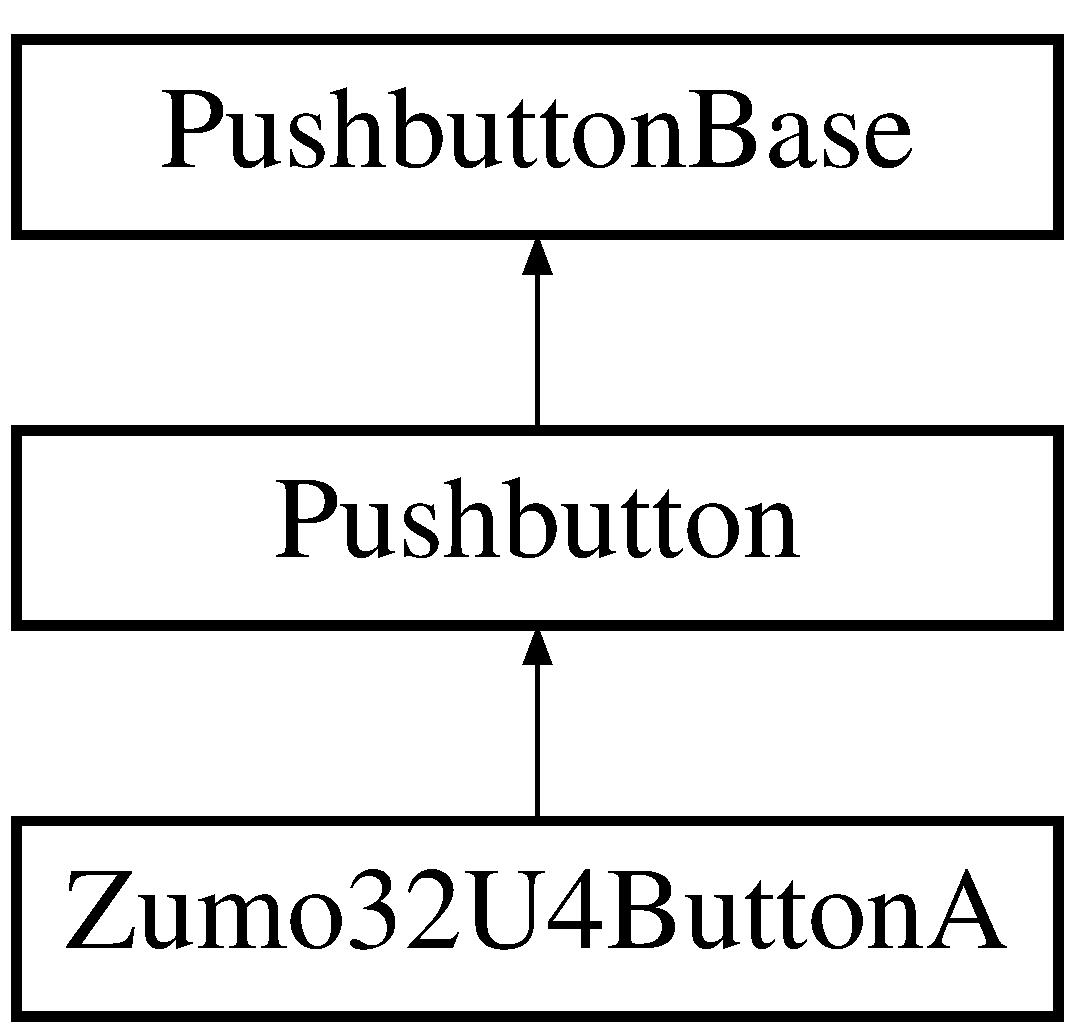
\includegraphics[height=3.000000cm]{class_pushbutton}
\end{center}
\end{figure}
\doxysubsection*{Public Member Functions}
\begin{DoxyCompactItemize}
\item 
\mbox{\hyperlink{class_pushbutton_a73d08312ffb3502580485d3d2051e19f}{Pushbutton}} (uint8\+\_\+t pin, uint8\+\_\+t pull\+Up=\mbox{\hyperlink{_pushbutton_8h_a2556d56311dd94f5834ef8fb4e6d875d}{PULL\+\_\+\+UP\+\_\+\+ENABLED}}, uint8\+\_\+t default\+State=\mbox{\hyperlink{_pushbutton_8h_ad0c2918a36a770522d44451389d22f34}{DEFAULT\+\_\+\+STATE\+\_\+\+HIGH}})
\item 
virtual bool \mbox{\hyperlink{class_pushbutton_a4990786220489fb5b6cf3af19b601a24}{is\+Pressed}} ()
\begin{DoxyCompactList}\small\item\em indicates whether button is currently pressed without any debouncing. \end{DoxyCompactList}\item 
void \mbox{\hyperlink{class_pushbutton_base_a2e2787595c82ee0913ecf4c1eea4a2c8}{wait\+For\+Press}} ()
\begin{DoxyCompactList}\small\item\em Waits until the button is pressed and takes care of debouncing. \end{DoxyCompactList}\item 
void \mbox{\hyperlink{class_pushbutton_base_ae5fff34b3e1ebd62fd02b99edd6bf13a}{wait\+For\+Release}} ()
\begin{DoxyCompactList}\small\item\em Waits until the button is released and takes care of debouncing. \end{DoxyCompactList}\item 
void \mbox{\hyperlink{class_pushbutton_base_ab755065c930be0649597220316213e8a}{wait\+For\+Button}} ()
\begin{DoxyCompactList}\small\item\em Waits until the button is pressed and then waits until the button is released, taking care of debouncing. \end{DoxyCompactList}\item 
bool \mbox{\hyperlink{class_pushbutton_base_a93953875c8b1c5f69dec3984774de296}{get\+Single\+Debounced\+Press}} ()
\begin{DoxyCompactList}\small\item\em Uses a state machine to return true once after each time it detects the button moving from the released state to the pressed state. \end{DoxyCompactList}\item 
bool \mbox{\hyperlink{class_pushbutton_base_ae568f5db0e8804247e0dcab72a311d42}{get\+Single\+Debounced\+Release}} ()
\begin{DoxyCompactList}\small\item\em Uses a state machine to return true once after each time it detects the button moving from the pressed state to the released state. \end{DoxyCompactList}\end{DoxyCompactItemize}


\doxysubsection{Detailed Description}
Main class for interfacing with pushbuttons. 

This class can interface with any pushbutton whose state can be read with the {\ttfamily digital\+Read} function, which is part of the Arduino core.

See \href{https://github.com/pololu/pushbutton-arduino}{\texttt{ https\+://github.\+com/pololu/pushbutton-\/arduino}} for an overview of the different ways to use this class. 

Definition at line 137 of file Pushbutton.\+h.



\doxysubsection{Constructor \& Destructor Documentation}
\mbox{\Hypertarget{class_pushbutton_a73d08312ffb3502580485d3d2051e19f}\label{class_pushbutton_a73d08312ffb3502580485d3d2051e19f}} 
\index{Pushbutton@{Pushbutton}!Pushbutton@{Pushbutton}}
\index{Pushbutton@{Pushbutton}!Pushbutton@{Pushbutton}}
\doxysubsubsection{\texorpdfstring{Pushbutton()}{Pushbutton()}}
{\footnotesize\ttfamily Pushbutton\+::\+Pushbutton (\begin{DoxyParamCaption}\item[{uint8\+\_\+t}]{pin,  }\item[{uint8\+\_\+t}]{pull\+Up = {\ttfamily \mbox{\hyperlink{_pushbutton_8h_a2556d56311dd94f5834ef8fb4e6d875d}{PULL\+\_\+\+UP\+\_\+\+ENABLED}}},  }\item[{uint8\+\_\+t}]{default\+State = {\ttfamily \mbox{\hyperlink{_pushbutton_8h_ad0c2918a36a770522d44451389d22f34}{DEFAULT\+\_\+\+STATE\+\_\+\+HIGH}}} }\end{DoxyParamCaption})}

Constructs a new instance of \mbox{\hyperlink{class_pushbutton}{Pushbutton}}.


\begin{DoxyParams}{Parameters}
{\em pin} & The pin number of the pin. This is used as an argument to {\ttfamily pin\+Mode} and {\ttfamily digital\+Read}.\\
\hline
{\em pull\+Up} & Specifies whether the pin\textquotesingle{}s internal pull-\/up resistor should be enabled. This should be either \mbox{\hyperlink{_pushbutton_8h_a2556d56311dd94f5834ef8fb4e6d875d}{PULL\+\_\+\+UP\+\_\+\+ENABLED}} (which is the default if the argument is omitted) or \mbox{\hyperlink{_pushbutton_8h_aa2df433ea6e6c6cd49babd945e27315e}{PULL\+\_\+\+UP\+\_\+\+DISABLED}}.\\
\hline
{\em default\+State} & Specifies the voltage level that corresponds to the button\textquotesingle{}s default (released) state. This should be either \mbox{\hyperlink{_pushbutton_8h_ad0c2918a36a770522d44451389d22f34}{DEFAULT\+\_\+\+STATE\+\_\+\+HIGH}} (which is the default if this argument is omitted) or \mbox{\hyperlink{_pushbutton_8h_ad1f5e860e74b4340ad61eb6b7f7d5406}{DEFAULT\+\_\+\+STATE\+\_\+\+LOW}}. \\
\hline
\end{DoxyParams}


Definition at line 120 of file Pushbutton.\+cpp.



\doxysubsection{Member Function Documentation}
\mbox{\Hypertarget{class_pushbutton_base_a93953875c8b1c5f69dec3984774de296}\label{class_pushbutton_base_a93953875c8b1c5f69dec3984774de296}} 
\index{Pushbutton@{Pushbutton}!getSingleDebouncedPress@{getSingleDebouncedPress}}
\index{getSingleDebouncedPress@{getSingleDebouncedPress}!Pushbutton@{Pushbutton}}
\doxysubsubsection{\texorpdfstring{getSingleDebouncedPress()}{getSingleDebouncedPress()}}
{\footnotesize\ttfamily bool Pushbutton\+Base\+::get\+Single\+Debounced\+Press (\begin{DoxyParamCaption}{ }\end{DoxyParamCaption})\hspace{0.3cm}{\ttfamily [inherited]}}



Uses a state machine to return true once after each time it detects the button moving from the released state to the pressed state. 

This is a non-\/blocking function that is meant to be called repeatedly in a loop. Each time it is called, it updates a state machine that monitors the state of the button. When it detects the button changing from the released state to the pressed state, with debouncing, it returns true. 

Definition at line 110 of file Pushbutton.\+cpp.

\mbox{\Hypertarget{class_pushbutton_base_ae568f5db0e8804247e0dcab72a311d42}\label{class_pushbutton_base_ae568f5db0e8804247e0dcab72a311d42}} 
\index{Pushbutton@{Pushbutton}!getSingleDebouncedRelease@{getSingleDebouncedRelease}}
\index{getSingleDebouncedRelease@{getSingleDebouncedRelease}!Pushbutton@{Pushbutton}}
\doxysubsubsection{\texorpdfstring{getSingleDebouncedRelease()}{getSingleDebouncedRelease()}}
{\footnotesize\ttfamily bool Pushbutton\+Base\+::get\+Single\+Debounced\+Release (\begin{DoxyParamCaption}{ }\end{DoxyParamCaption})\hspace{0.3cm}{\ttfamily [inherited]}}



Uses a state machine to return true once after each time it detects the button moving from the pressed state to the released state. 

This is just like \mbox{\hyperlink{class_pushbutton_base_a93953875c8b1c5f69dec3984774de296}{get\+Single\+Debounced\+Press()}} except it has a separate state machine and it watches for when the button goes from the pressed state to the released state.

There is no strict guarantee that every debounced button press event returned by \mbox{\hyperlink{class_pushbutton_base_a93953875c8b1c5f69dec3984774de296}{get\+Single\+Debounced\+Press()}} will have a corresponding button release event returned by \mbox{\hyperlink{class_pushbutton_base_ae568f5db0e8804247e0dcab72a311d42}{get\+Single\+Debounced\+Release()}}; the two functions use independent state machines and sample the button at different times. 

Definition at line 115 of file Pushbutton.\+cpp.

\mbox{\Hypertarget{class_pushbutton_a4990786220489fb5b6cf3af19b601a24}\label{class_pushbutton_a4990786220489fb5b6cf3af19b601a24}} 
\index{Pushbutton@{Pushbutton}!isPressed@{isPressed}}
\index{isPressed@{isPressed}!Pushbutton@{Pushbutton}}
\doxysubsubsection{\texorpdfstring{isPressed()}{isPressed()}}
{\footnotesize\ttfamily bool Pushbutton\+::is\+Pressed (\begin{DoxyParamCaption}{ }\end{DoxyParamCaption})\hspace{0.3cm}{\ttfamily [virtual]}}



indicates whether button is currently pressed without any debouncing. 

\begin{DoxyReturn}{Returns}
1 if the button is pressed right now, 0 if it is not.
\end{DoxyReturn}
This function must be implemented in a subclass of \mbox{\hyperlink{class_pushbutton_base}{Pushbutton\+Base}}, such as \mbox{\hyperlink{class_pushbutton}{Pushbutton}}. 

Implements \mbox{\hyperlink{class_pushbutton_base_a5b11851f15413140b75e4574e773b6ae}{Pushbutton\+Base}}.



Definition at line 142 of file Pushbutton.\+cpp.

\mbox{\Hypertarget{class_pushbutton_base_ab755065c930be0649597220316213e8a}\label{class_pushbutton_base_ab755065c930be0649597220316213e8a}} 
\index{Pushbutton@{Pushbutton}!waitForButton@{waitForButton}}
\index{waitForButton@{waitForButton}!Pushbutton@{Pushbutton}}
\doxysubsubsection{\texorpdfstring{waitForButton()}{waitForButton()}}
{\footnotesize\ttfamily void Pushbutton\+Base\+::wait\+For\+Button (\begin{DoxyParamCaption}{ }\end{DoxyParamCaption})\hspace{0.3cm}{\ttfamily [inherited]}}



Waits until the button is pressed and then waits until the button is released, taking care of debouncing. 

This is equivalent to calling \mbox{\hyperlink{class_pushbutton_base_a2e2787595c82ee0913ecf4c1eea4a2c8}{wait\+For\+Press()}} and then \mbox{\hyperlink{class_pushbutton_base_ae5fff34b3e1ebd62fd02b99edd6bf13a}{wait\+For\+Release()}}. 

Definition at line 104 of file Pushbutton.\+cpp.

\mbox{\Hypertarget{class_pushbutton_base_a2e2787595c82ee0913ecf4c1eea4a2c8}\label{class_pushbutton_base_a2e2787595c82ee0913ecf4c1eea4a2c8}} 
\index{Pushbutton@{Pushbutton}!waitForPress@{waitForPress}}
\index{waitForPress@{waitForPress}!Pushbutton@{Pushbutton}}
\doxysubsubsection{\texorpdfstring{waitForPress()}{waitForPress()}}
{\footnotesize\ttfamily void Pushbutton\+Base\+::wait\+For\+Press (\begin{DoxyParamCaption}{ }\end{DoxyParamCaption})\hspace{0.3cm}{\ttfamily [inherited]}}



Waits until the button is pressed and takes care of debouncing. 

This function waits until the button is in the pressed state and then returns. Note that if the button is already pressed when you call this function, it will return quickly (in 10 ms). 

Definition at line 84 of file Pushbutton.\+cpp.

\mbox{\Hypertarget{class_pushbutton_base_ae5fff34b3e1ebd62fd02b99edd6bf13a}\label{class_pushbutton_base_ae5fff34b3e1ebd62fd02b99edd6bf13a}} 
\index{Pushbutton@{Pushbutton}!waitForRelease@{waitForRelease}}
\index{waitForRelease@{waitForRelease}!Pushbutton@{Pushbutton}}
\doxysubsubsection{\texorpdfstring{waitForRelease()}{waitForRelease()}}
{\footnotesize\ttfamily void Pushbutton\+Base\+::wait\+For\+Release (\begin{DoxyParamCaption}{ }\end{DoxyParamCaption})\hspace{0.3cm}{\ttfamily [inherited]}}



Waits until the button is released and takes care of debouncing. 

This function waits until the button is in the released state and then returns. Note that if the button is already released when you call this function, it will return quickly (in 10 ms). 

Definition at line 94 of file Pushbutton.\+cpp.



The documentation for this class was generated from the following files\+:\begin{DoxyCompactItemize}
\item 
\mbox{\hyperlink{_pushbutton_8h}{Pushbutton.\+h}}\item 
Pushbutton.\+cpp\end{DoxyCompactItemize}

\hypertarget{class_pushbutton_base}{}\doxysection{Pushbutton\+Base Class Reference}
\label{class_pushbutton_base}\index{PushbuttonBase@{PushbuttonBase}}


General pushbutton class that handles debouncing.  




{\ttfamily \#include $<$Pushbutton.\+h$>$}

Inheritance diagram for Pushbutton\+Base\+:\begin{figure}[H]
\begin{center}
\leavevmode
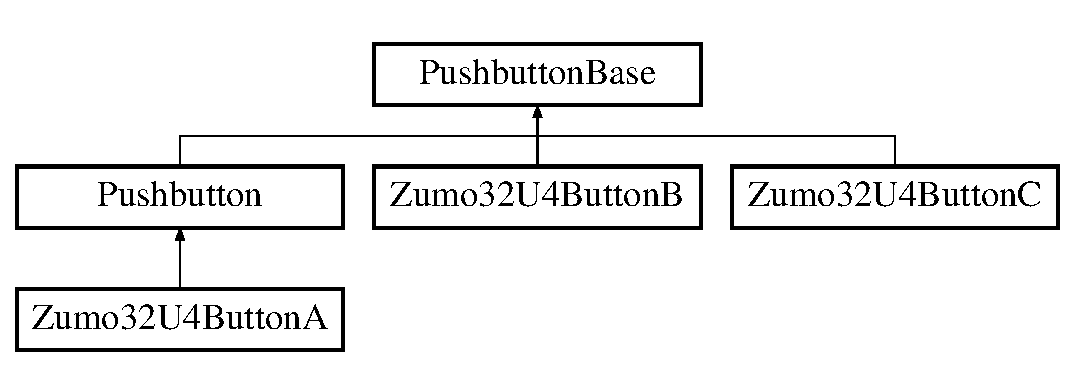
\includegraphics[height=3.000000cm]{class_pushbutton_base}
\end{center}
\end{figure}
\doxysubsection*{Public Member Functions}
\begin{DoxyCompactItemize}
\item 
void \mbox{\hyperlink{class_pushbutton_base_a2e2787595c82ee0913ecf4c1eea4a2c8}{wait\+For\+Press}} ()
\begin{DoxyCompactList}\small\item\em Waits until the button is pressed and takes care of debouncing. \end{DoxyCompactList}\item 
void \mbox{\hyperlink{class_pushbutton_base_ae5fff34b3e1ebd62fd02b99edd6bf13a}{wait\+For\+Release}} ()
\begin{DoxyCompactList}\small\item\em Waits until the button is released and takes care of debouncing. \end{DoxyCompactList}\item 
void \mbox{\hyperlink{class_pushbutton_base_ab755065c930be0649597220316213e8a}{wait\+For\+Button}} ()
\begin{DoxyCompactList}\small\item\em Waits until the button is pressed and then waits until the button is released, taking care of debouncing. \end{DoxyCompactList}\item 
bool \mbox{\hyperlink{class_pushbutton_base_a93953875c8b1c5f69dec3984774de296}{get\+Single\+Debounced\+Press}} ()
\begin{DoxyCompactList}\small\item\em Uses a state machine to return true once after each time it detects the button moving from the released state to the pressed state. \end{DoxyCompactList}\item 
bool \mbox{\hyperlink{class_pushbutton_base_ae568f5db0e8804247e0dcab72a311d42}{get\+Single\+Debounced\+Release}} ()
\begin{DoxyCompactList}\small\item\em Uses a state machine to return true once after each time it detects the button moving from the pressed state to the released state. \end{DoxyCompactList}\item 
virtual bool \mbox{\hyperlink{class_pushbutton_base_a5b11851f15413140b75e4574e773b6ae}{is\+Pressed}} ()=0
\begin{DoxyCompactList}\small\item\em indicates whether button is currently pressed without any debouncing. \end{DoxyCompactList}\end{DoxyCompactItemize}


\doxysubsection{Detailed Description}
General pushbutton class that handles debouncing. 

/$\ast$!

This is an abstract class used for interfacing with pushbuttons. It knows about debouncing, but it knows nothing about how to read the current state of the button. The functions in this class get the current state of the button by calling \mbox{\hyperlink{class_pushbutton_base_a5b11851f15413140b75e4574e773b6ae}{is\+Pressed()}}, a virtual function which must be implemented in a subclass of \mbox{\hyperlink{class_pushbutton_base}{Pushbutton\+Base}}, such as \mbox{\hyperlink{class_pushbutton}{Pushbutton}}.

Most users of this library do not need to directly use \mbox{\hyperlink{class_pushbutton_base}{Pushbutton\+Base}} or even know that it exists. They can use \mbox{\hyperlink{class_pushbutton}{Pushbutton}} instead. 

Definition at line \mbox{\hyperlink{_pushbutton_8h_source_l00070}{70}} of file \mbox{\hyperlink{_pushbutton_8h_source}{Pushbutton.\+h}}.



\doxysubsection{Member Function Documentation}
\mbox{\Hypertarget{class_pushbutton_base_a93953875c8b1c5f69dec3984774de296}\label{class_pushbutton_base_a93953875c8b1c5f69dec3984774de296}} 
\index{PushbuttonBase@{PushbuttonBase}!getSingleDebouncedPress@{getSingleDebouncedPress}}
\index{getSingleDebouncedPress@{getSingleDebouncedPress}!PushbuttonBase@{PushbuttonBase}}
\doxysubsubsection{\texorpdfstring{getSingleDebouncedPress()}{getSingleDebouncedPress()}}
{\footnotesize\ttfamily bool Pushbutton\+Base\+::get\+Single\+Debounced\+Press (\begin{DoxyParamCaption}{ }\end{DoxyParamCaption})}



Uses a state machine to return true once after each time it detects the button moving from the released state to the pressed state. 

This is a non-\/blocking function that is meant to be called repeatedly in a loop. Each time it is called, it updates a state machine that monitors the state of the button. When it detects the button changing from the released state to the pressed state, with debouncing, it returns true. 

Definition at line \mbox{\hyperlink{_pushbutton_8cpp_source_l00110}{110}} of file \mbox{\hyperlink{_pushbutton_8cpp_source}{Pushbutton.\+cpp}}.

\mbox{\Hypertarget{class_pushbutton_base_ae568f5db0e8804247e0dcab72a311d42}\label{class_pushbutton_base_ae568f5db0e8804247e0dcab72a311d42}} 
\index{PushbuttonBase@{PushbuttonBase}!getSingleDebouncedRelease@{getSingleDebouncedRelease}}
\index{getSingleDebouncedRelease@{getSingleDebouncedRelease}!PushbuttonBase@{PushbuttonBase}}
\doxysubsubsection{\texorpdfstring{getSingleDebouncedRelease()}{getSingleDebouncedRelease()}}
{\footnotesize\ttfamily bool Pushbutton\+Base\+::get\+Single\+Debounced\+Release (\begin{DoxyParamCaption}{ }\end{DoxyParamCaption})}



Uses a state machine to return true once after each time it detects the button moving from the pressed state to the released state. 

This is just like \mbox{\hyperlink{class_pushbutton_base_a93953875c8b1c5f69dec3984774de296}{get\+Single\+Debounced\+Press()}} except it has a separate state machine and it watches for when the button goes from the pressed state to the released state.

There is no strict guarantee that every debounced button press event returned by \mbox{\hyperlink{class_pushbutton_base_a93953875c8b1c5f69dec3984774de296}{get\+Single\+Debounced\+Press()}} will have a corresponding button release event returned by \mbox{\hyperlink{class_pushbutton_base_ae568f5db0e8804247e0dcab72a311d42}{get\+Single\+Debounced\+Release()}}; the two functions use independent state machines and sample the button at different times. 

Definition at line \mbox{\hyperlink{_pushbutton_8cpp_source_l00115}{115}} of file \mbox{\hyperlink{_pushbutton_8cpp_source}{Pushbutton.\+cpp}}.

\mbox{\Hypertarget{class_pushbutton_base_a5b11851f15413140b75e4574e773b6ae}\label{class_pushbutton_base_a5b11851f15413140b75e4574e773b6ae}} 
\index{PushbuttonBase@{PushbuttonBase}!isPressed@{isPressed}}
\index{isPressed@{isPressed}!PushbuttonBase@{PushbuttonBase}}
\doxysubsubsection{\texorpdfstring{isPressed()}{isPressed()}}
{\footnotesize\ttfamily virtual bool Pushbutton\+Base\+::is\+Pressed (\begin{DoxyParamCaption}{ }\end{DoxyParamCaption})\hspace{0.3cm}{\ttfamily [pure virtual]}}



indicates whether button is currently pressed without any debouncing. 

\begin{DoxyReturn}{Returns}
1 if the button is pressed right now, 0 if it is not.
\end{DoxyReturn}
This function must be implemented in a subclass of \mbox{\hyperlink{class_pushbutton_base}{Pushbutton\+Base}}, such as \mbox{\hyperlink{class_pushbutton}{Pushbutton}}. 

Implemented in \mbox{\hyperlink{class_pushbutton_a4990786220489fb5b6cf3af19b601a24}{Pushbutton}}, \mbox{\hyperlink{class_zumo32_u4_button_b_a013a2c0029356aece18b93963373a736}{Zumo32\+U4\+ButtonB}}, and \mbox{\hyperlink{class_zumo32_u4_button_c_aa75e220cde340487a3fa8f1f99d645f8}{Zumo32\+U4\+ButtonC}}.

\mbox{\Hypertarget{class_pushbutton_base_ab755065c930be0649597220316213e8a}\label{class_pushbutton_base_ab755065c930be0649597220316213e8a}} 
\index{PushbuttonBase@{PushbuttonBase}!waitForButton@{waitForButton}}
\index{waitForButton@{waitForButton}!PushbuttonBase@{PushbuttonBase}}
\doxysubsubsection{\texorpdfstring{waitForButton()}{waitForButton()}}
{\footnotesize\ttfamily void Pushbutton\+Base\+::wait\+For\+Button (\begin{DoxyParamCaption}{ }\end{DoxyParamCaption})}



Waits until the button is pressed and then waits until the button is released, taking care of debouncing. 

This is equivalent to calling \mbox{\hyperlink{class_pushbutton_base_a2e2787595c82ee0913ecf4c1eea4a2c8}{wait\+For\+Press()}} and then \mbox{\hyperlink{class_pushbutton_base_ae5fff34b3e1ebd62fd02b99edd6bf13a}{wait\+For\+Release()}}. 

Definition at line \mbox{\hyperlink{_pushbutton_8cpp_source_l00104}{104}} of file \mbox{\hyperlink{_pushbutton_8cpp_source}{Pushbutton.\+cpp}}.

\mbox{\Hypertarget{class_pushbutton_base_a2e2787595c82ee0913ecf4c1eea4a2c8}\label{class_pushbutton_base_a2e2787595c82ee0913ecf4c1eea4a2c8}} 
\index{PushbuttonBase@{PushbuttonBase}!waitForPress@{waitForPress}}
\index{waitForPress@{waitForPress}!PushbuttonBase@{PushbuttonBase}}
\doxysubsubsection{\texorpdfstring{waitForPress()}{waitForPress()}}
{\footnotesize\ttfamily void Pushbutton\+Base\+::wait\+For\+Press (\begin{DoxyParamCaption}{ }\end{DoxyParamCaption})}



Waits until the button is pressed and takes care of debouncing. 

This function waits until the button is in the pressed state and then returns. Note that if the button is already pressed when you call this function, it will return quickly (in 10 ms). 

Definition at line \mbox{\hyperlink{_pushbutton_8cpp_source_l00084}{84}} of file \mbox{\hyperlink{_pushbutton_8cpp_source}{Pushbutton.\+cpp}}.

\mbox{\Hypertarget{class_pushbutton_base_ae5fff34b3e1ebd62fd02b99edd6bf13a}\label{class_pushbutton_base_ae5fff34b3e1ebd62fd02b99edd6bf13a}} 
\index{PushbuttonBase@{PushbuttonBase}!waitForRelease@{waitForRelease}}
\index{waitForRelease@{waitForRelease}!PushbuttonBase@{PushbuttonBase}}
\doxysubsubsection{\texorpdfstring{waitForRelease()}{waitForRelease()}}
{\footnotesize\ttfamily void Pushbutton\+Base\+::wait\+For\+Release (\begin{DoxyParamCaption}{ }\end{DoxyParamCaption})}



Waits until the button is released and takes care of debouncing. 

This function waits until the button is in the released state and then returns. Note that if the button is already released when you call this function, it will return quickly (in 10 ms). 

Definition at line \mbox{\hyperlink{_pushbutton_8cpp_source_l00094}{94}} of file \mbox{\hyperlink{_pushbutton_8cpp_source}{Pushbutton.\+cpp}}.



The documentation for this class was generated from the following files\+:\begin{DoxyCompactItemize}
\item 
\mbox{\hyperlink{_pushbutton_8h}{Pushbutton.\+h}}\item 
Pushbutton.\+cpp\end{DoxyCompactItemize}

\hypertarget{class_q_t_r_sensors}{}\doxysection{QTRSensors Class Reference}
\label{class_q_t_r_sensors}\index{QTRSensors@{QTRSensors}}
Inheritance diagram for QTRSensors\+:\begin{figure}[H]
\begin{center}
\leavevmode
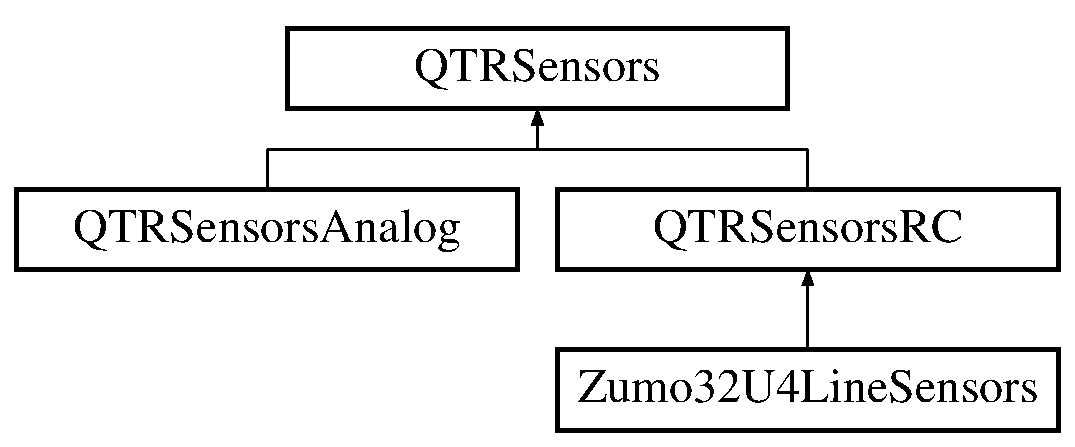
\includegraphics[height=3.000000cm]{class_q_t_r_sensors}
\end{center}
\end{figure}
\doxysubsection*{Public Member Functions}
\begin{DoxyCompactItemize}
\item 
void \mbox{\hyperlink{class_q_t_r_sensors_afc47e6c2608293a610e1a3acce93628b}{read}} (unsigned int $\ast$sensor\+\_\+values, unsigned char read\+Mode=QTR\+\_\+\+EMITTERS\+\_\+\+ON)
\item 
void \mbox{\hyperlink{class_q_t_r_sensors_a576f1fe1e9f2d3d2097baf79a9655134}{emitters\+Off}} ()
\item 
void \mbox{\hyperlink{class_q_t_r_sensors_a79f5380ecdb324a7800a045c3506975f}{emitters\+On}} ()
\item 
void \mbox{\hyperlink{class_q_t_r_sensors_ac9840e2429c7a962977057ba154c77da}{calibrate}} (unsigned char read\+Mode=QTR\+\_\+\+EMITTERS\+\_\+\+ON)
\item 
void \mbox{\hyperlink{class_q_t_r_sensors_aa840b6ef17562d41edf21ddd08e0672e}{reset\+Calibration}} ()
\item 
void \mbox{\hyperlink{class_q_t_r_sensors_aa32a448ac03cd2a45d1f14f96ac4b739}{read\+Calibrated}} (unsigned int $\ast$sensor\+\_\+values, unsigned char read\+Mode=QTR\+\_\+\+EMITTERS\+\_\+\+ON)
\item 
int \mbox{\hyperlink{class_q_t_r_sensors_ac84f0b98bceae0b59d687ae82eb92718}{read\+Line}} (unsigned int $\ast$sensor\+\_\+values, unsigned char read\+Mode=QTR\+\_\+\+EMITTERS\+\_\+\+ON, unsigned char white\+\_\+line=0)
\end{DoxyCompactItemize}
\doxysubsection*{Public Attributes}
\begin{DoxyCompactItemize}
\item 
unsigned int $\ast$ \mbox{\hyperlink{class_q_t_r_sensors_a9308c21df0015965dceb9dd1f570f78d}{calibrated\+Minimum\+On}}
\item 
unsigned int $\ast$ \mbox{\hyperlink{class_q_t_r_sensors_ab7a739d5bb85b17e94e825454cc63195}{calibrated\+Maximum\+On}}
\item 
unsigned int $\ast$ \mbox{\hyperlink{class_q_t_r_sensors_af299d7e4a7900f4f3d5e567a10f4ab16}{calibrated\+Minimum\+Off}}
\item 
unsigned int $\ast$ \mbox{\hyperlink{class_q_t_r_sensors_a75af08628235c3ec5d4414a6032a016c}{calibrated\+Maximum\+Off}}
\end{DoxyCompactItemize}
\doxysubsection*{Protected Member Functions}
\begin{DoxyCompactItemize}
\item 
void \mbox{\hyperlink{class_q_t_r_sensors_ae1d5eb9479d4dee1977109b17aece70e}{init}} (unsigned char $\ast$pins, unsigned char num\+Sensors, unsigned char emitter\+Pin)
\end{DoxyCompactItemize}
\doxysubsection*{Protected Attributes}
\begin{DoxyCompactItemize}
\item 
unsigned char $\ast$ \mbox{\hyperlink{class_q_t_r_sensors_ad22b7f2b4778133efa1967d683e5cb46}{\+\_\+pins}}
\item 
unsigned char \mbox{\hyperlink{class_q_t_r_sensors_af4e3b5b4b9fd7acb0914a9f345e446f0}{\+\_\+num\+Sensors}}
\item 
unsigned char \mbox{\hyperlink{class_q_t_r_sensors_a116880e22fe5e5c474e021b91e04e2ac}{\+\_\+emitter\+Pin}}
\item 
unsigned int \mbox{\hyperlink{class_q_t_r_sensors_a88657f1405aa7dc840f2025b53e1a4b3}{\+\_\+max\+Value}}
\item 
int \mbox{\hyperlink{class_q_t_r_sensors_a9c3c8b7ac645020c77ff8198145b46b6}{\+\_\+last\+Value}}
\end{DoxyCompactItemize}


\doxysubsection{Detailed Description}


Definition at line \mbox{\hyperlink{_q_t_r_sensors_8h_source_l00048}{48}} of file \mbox{\hyperlink{_q_t_r_sensors_8h_source}{QTRSensors.\+h}}.



\doxysubsection{Constructor \& Destructor Documentation}
\mbox{\Hypertarget{class_q_t_r_sensors_a2e4867e3b89ec1387a97a7ba13bf9216}\label{class_q_t_r_sensors_a2e4867e3b89ec1387a97a7ba13bf9216}} 
\index{QTRSensors@{QTRSensors}!````~QTRSensors@{$\sim$QTRSensors}}
\index{````~QTRSensors@{$\sim$QTRSensors}!QTRSensors@{QTRSensors}}
\doxysubsubsection{\texorpdfstring{$\sim$QTRSensors()}{~QTRSensors()}}
{\footnotesize\ttfamily QTRSensors\+::$\sim$\+QTRSensors (\begin{DoxyParamCaption}{ }\end{DoxyParamCaption})}



Definition at line \mbox{\hyperlink{_q_t_r_sensors_8cpp_source_l00552}{552}} of file \mbox{\hyperlink{_q_t_r_sensors_8cpp_source}{QTRSensors.\+cpp}}.

\mbox{\Hypertarget{class_q_t_r_sensors_af0c8e47e146955ef6711b8fc1e6cbac4}\label{class_q_t_r_sensors_af0c8e47e146955ef6711b8fc1e6cbac4}} 
\index{QTRSensors@{QTRSensors}!QTRSensors@{QTRSensors}}
\index{QTRSensors@{QTRSensors}!QTRSensors@{QTRSensors}}
\doxysubsubsection{\texorpdfstring{QTRSensors()}{QTRSensors()}}
{\footnotesize\ttfamily QTRSensors\+::\+QTRSensors (\begin{DoxyParamCaption}{ }\end{DoxyParamCaption})\hspace{0.3cm}{\ttfamily [inline]}, {\ttfamily [protected]}}



Definition at line \mbox{\hyperlink{_q_t_r_sensors_8h_source_l00133}{133}} of file \mbox{\hyperlink{_q_t_r_sensors_8h_source}{QTRSensors.\+h}}.



\doxysubsection{Member Function Documentation}
\mbox{\Hypertarget{class_q_t_r_sensors_ac9840e2429c7a962977057ba154c77da}\label{class_q_t_r_sensors_ac9840e2429c7a962977057ba154c77da}} 
\index{QTRSensors@{QTRSensors}!calibrate@{calibrate}}
\index{calibrate@{calibrate}!QTRSensors@{QTRSensors}}
\doxysubsubsection{\texorpdfstring{calibrate()}{calibrate()}}
{\footnotesize\ttfamily void QTRSensors\+::calibrate (\begin{DoxyParamCaption}\item[{unsigned char}]{read\+Mode = {\ttfamily QTR\+\_\+EMITTERS\+\_\+ON} }\end{DoxyParamCaption})}



Definition at line \mbox{\hyperlink{_q_t_r_sensors_8cpp_source_l00149}{149}} of file \mbox{\hyperlink{_q_t_r_sensors_8cpp_source}{QTRSensors.\+cpp}}.

\mbox{\Hypertarget{class_q_t_r_sensors_a576f1fe1e9f2d3d2097baf79a9655134}\label{class_q_t_r_sensors_a576f1fe1e9f2d3d2097baf79a9655134}} 
\index{QTRSensors@{QTRSensors}!emittersOff@{emittersOff}}
\index{emittersOff@{emittersOff}!QTRSensors@{QTRSensors}}
\doxysubsubsection{\texorpdfstring{emittersOff()}{emittersOff()}}
{\footnotesize\ttfamily void QTRSensors\+::emitters\+Off (\begin{DoxyParamCaption}{ }\end{DoxyParamCaption})}



Definition at line \mbox{\hyperlink{_q_t_r_sensors_8cpp_source_l00110}{110}} of file \mbox{\hyperlink{_q_t_r_sensors_8cpp_source}{QTRSensors.\+cpp}}.

\mbox{\Hypertarget{class_q_t_r_sensors_a79f5380ecdb324a7800a045c3506975f}\label{class_q_t_r_sensors_a79f5380ecdb324a7800a045c3506975f}} 
\index{QTRSensors@{QTRSensors}!emittersOn@{emittersOn}}
\index{emittersOn@{emittersOn}!QTRSensors@{QTRSensors}}
\doxysubsubsection{\texorpdfstring{emittersOn()}{emittersOn()}}
{\footnotesize\ttfamily void QTRSensors\+::emitters\+On (\begin{DoxyParamCaption}{ }\end{DoxyParamCaption})}



Definition at line \mbox{\hyperlink{_q_t_r_sensors_8cpp_source_l00119}{119}} of file \mbox{\hyperlink{_q_t_r_sensors_8cpp_source}{QTRSensors.\+cpp}}.

\mbox{\Hypertarget{class_q_t_r_sensors_ae1d5eb9479d4dee1977109b17aece70e}\label{class_q_t_r_sensors_ae1d5eb9479d4dee1977109b17aece70e}} 
\index{QTRSensors@{QTRSensors}!init@{init}}
\index{init@{init}!QTRSensors@{QTRSensors}}
\doxysubsubsection{\texorpdfstring{init()}{init()}}
{\footnotesize\ttfamily void QTRSensors\+::init (\begin{DoxyParamCaption}\item[{unsigned char $\ast$}]{pins,  }\item[{unsigned char}]{num\+Sensors,  }\item[{unsigned char}]{emitter\+Pin }\end{DoxyParamCaption})\hspace{0.3cm}{\ttfamily [protected]}}



Definition at line \mbox{\hyperlink{_q_t_r_sensors_8cpp_source_l00041}{41}} of file \mbox{\hyperlink{_q_t_r_sensors_8cpp_source}{QTRSensors.\+cpp}}.

\mbox{\Hypertarget{class_q_t_r_sensors_afc47e6c2608293a610e1a3acce93628b}\label{class_q_t_r_sensors_afc47e6c2608293a610e1a3acce93628b}} 
\index{QTRSensors@{QTRSensors}!read@{read}}
\index{read@{read}!QTRSensors@{QTRSensors}}
\doxysubsubsection{\texorpdfstring{read()}{read()}}
{\footnotesize\ttfamily void QTRSensors\+::read (\begin{DoxyParamCaption}\item[{unsigned int $\ast$}]{sensor\+\_\+values,  }\item[{unsigned char}]{read\+Mode = {\ttfamily QTR\+\_\+EMITTERS\+\_\+ON} }\end{DoxyParamCaption})}



Definition at line \mbox{\hyperlink{_q_t_r_sensors_8cpp_source_l00081}{81}} of file \mbox{\hyperlink{_q_t_r_sensors_8cpp_source}{QTRSensors.\+cpp}}.

\mbox{\Hypertarget{class_q_t_r_sensors_aa32a448ac03cd2a45d1f14f96ac4b739}\label{class_q_t_r_sensors_aa32a448ac03cd2a45d1f14f96ac4b739}} 
\index{QTRSensors@{QTRSensors}!readCalibrated@{readCalibrated}}
\index{readCalibrated@{readCalibrated}!QTRSensors@{QTRSensors}}
\doxysubsubsection{\texorpdfstring{readCalibrated()}{readCalibrated()}}
{\footnotesize\ttfamily void QTRSensors\+::read\+Calibrated (\begin{DoxyParamCaption}\item[{unsigned int $\ast$}]{sensor\+\_\+values,  }\item[{unsigned char}]{read\+Mode = {\ttfamily QTR\+\_\+EMITTERS\+\_\+ON} }\end{DoxyParamCaption})}



Definition at line \mbox{\hyperlink{_q_t_r_sensors_8cpp_source_l00235}{235}} of file \mbox{\hyperlink{_q_t_r_sensors_8cpp_source}{QTRSensors.\+cpp}}.

\mbox{\Hypertarget{class_q_t_r_sensors_ac84f0b98bceae0b59d687ae82eb92718}\label{class_q_t_r_sensors_ac84f0b98bceae0b59d687ae82eb92718}} 
\index{QTRSensors@{QTRSensors}!readLine@{readLine}}
\index{readLine@{readLine}!QTRSensors@{QTRSensors}}
\doxysubsubsection{\texorpdfstring{readLine()}{readLine()}}
{\footnotesize\ttfamily int QTRSensors\+::read\+Line (\begin{DoxyParamCaption}\item[{unsigned int $\ast$}]{sensor\+\_\+values,  }\item[{unsigned char}]{read\+Mode = {\ttfamily QTR\+\_\+EMITTERS\+\_\+ON},  }\item[{unsigned char}]{white\+\_\+line = {\ttfamily 0} }\end{DoxyParamCaption})}



Definition at line \mbox{\hyperlink{_q_t_r_sensors_8cpp_source_l00315}{315}} of file \mbox{\hyperlink{_q_t_r_sensors_8cpp_source}{QTRSensors.\+cpp}}.

\mbox{\Hypertarget{class_q_t_r_sensors_aa840b6ef17562d41edf21ddd08e0672e}\label{class_q_t_r_sensors_aa840b6ef17562d41edf21ddd08e0672e}} 
\index{QTRSensors@{QTRSensors}!resetCalibration@{resetCalibration}}
\index{resetCalibration@{resetCalibration}!QTRSensors@{QTRSensors}}
\doxysubsubsection{\texorpdfstring{resetCalibration()}{resetCalibration()}}
{\footnotesize\ttfamily void QTRSensors\+::reset\+Calibration (\begin{DoxyParamCaption}{ }\end{DoxyParamCaption})}



Definition at line \mbox{\hyperlink{_q_t_r_sensors_8cpp_source_l00129}{129}} of file \mbox{\hyperlink{_q_t_r_sensors_8cpp_source}{QTRSensors.\+cpp}}.



\doxysubsection{Member Data Documentation}
\mbox{\Hypertarget{class_q_t_r_sensors_a116880e22fe5e5c474e021b91e04e2ac}\label{class_q_t_r_sensors_a116880e22fe5e5c474e021b91e04e2ac}} 
\index{QTRSensors@{QTRSensors}!\_emitterPin@{\_emitterPin}}
\index{\_emitterPin@{\_emitterPin}!QTRSensors@{QTRSensors}}
\doxysubsubsection{\texorpdfstring{\_emitterPin}{\_emitterPin}}
{\footnotesize\ttfamily unsigned char QTRSensors\+::\+\_\+emitter\+Pin\hspace{0.3cm}{\ttfamily [protected]}}



Definition at line \mbox{\hyperlink{_q_t_r_sensors_8h_source_l00142}{142}} of file \mbox{\hyperlink{_q_t_r_sensors_8h_source}{QTRSensors.\+h}}.

\mbox{\Hypertarget{class_q_t_r_sensors_a9c3c8b7ac645020c77ff8198145b46b6}\label{class_q_t_r_sensors_a9c3c8b7ac645020c77ff8198145b46b6}} 
\index{QTRSensors@{QTRSensors}!\_lastValue@{\_lastValue}}
\index{\_lastValue@{\_lastValue}!QTRSensors@{QTRSensors}}
\doxysubsubsection{\texorpdfstring{\_lastValue}{\_lastValue}}
{\footnotesize\ttfamily int QTRSensors\+::\+\_\+last\+Value\hspace{0.3cm}{\ttfamily [protected]}}



Definition at line \mbox{\hyperlink{_q_t_r_sensors_8h_source_l00144}{144}} of file \mbox{\hyperlink{_q_t_r_sensors_8h_source}{QTRSensors.\+h}}.

\mbox{\Hypertarget{class_q_t_r_sensors_a88657f1405aa7dc840f2025b53e1a4b3}\label{class_q_t_r_sensors_a88657f1405aa7dc840f2025b53e1a4b3}} 
\index{QTRSensors@{QTRSensors}!\_maxValue@{\_maxValue}}
\index{\_maxValue@{\_maxValue}!QTRSensors@{QTRSensors}}
\doxysubsubsection{\texorpdfstring{\_maxValue}{\_maxValue}}
{\footnotesize\ttfamily unsigned int QTRSensors\+::\+\_\+max\+Value\hspace{0.3cm}{\ttfamily [protected]}}



Definition at line \mbox{\hyperlink{_q_t_r_sensors_8h_source_l00143}{143}} of file \mbox{\hyperlink{_q_t_r_sensors_8h_source}{QTRSensors.\+h}}.

\mbox{\Hypertarget{class_q_t_r_sensors_af4e3b5b4b9fd7acb0914a9f345e446f0}\label{class_q_t_r_sensors_af4e3b5b4b9fd7acb0914a9f345e446f0}} 
\index{QTRSensors@{QTRSensors}!\_numSensors@{\_numSensors}}
\index{\_numSensors@{\_numSensors}!QTRSensors@{QTRSensors}}
\doxysubsubsection{\texorpdfstring{\_numSensors}{\_numSensors}}
{\footnotesize\ttfamily unsigned char QTRSensors\+::\+\_\+num\+Sensors\hspace{0.3cm}{\ttfamily [protected]}}



Definition at line \mbox{\hyperlink{_q_t_r_sensors_8h_source_l00141}{141}} of file \mbox{\hyperlink{_q_t_r_sensors_8h_source}{QTRSensors.\+h}}.

\mbox{\Hypertarget{class_q_t_r_sensors_ad22b7f2b4778133efa1967d683e5cb46}\label{class_q_t_r_sensors_ad22b7f2b4778133efa1967d683e5cb46}} 
\index{QTRSensors@{QTRSensors}!\_pins@{\_pins}}
\index{\_pins@{\_pins}!QTRSensors@{QTRSensors}}
\doxysubsubsection{\texorpdfstring{\_pins}{\_pins}}
{\footnotesize\ttfamily unsigned char$\ast$ QTRSensors\+::\+\_\+pins\hspace{0.3cm}{\ttfamily [protected]}}



Definition at line \mbox{\hyperlink{_q_t_r_sensors_8h_source_l00140}{140}} of file \mbox{\hyperlink{_q_t_r_sensors_8h_source}{QTRSensors.\+h}}.

\mbox{\Hypertarget{class_q_t_r_sensors_a75af08628235c3ec5d4414a6032a016c}\label{class_q_t_r_sensors_a75af08628235c3ec5d4414a6032a016c}} 
\index{QTRSensors@{QTRSensors}!calibratedMaximumOff@{calibratedMaximumOff}}
\index{calibratedMaximumOff@{calibratedMaximumOff}!QTRSensors@{QTRSensors}}
\doxysubsubsection{\texorpdfstring{calibratedMaximumOff}{calibratedMaximumOff}}
{\footnotesize\ttfamily unsigned int$\ast$ QTRSensors\+::calibrated\+Maximum\+Off}



Definition at line \mbox{\hyperlink{_q_t_r_sensors_8h_source_l00127}{127}} of file \mbox{\hyperlink{_q_t_r_sensors_8h_source}{QTRSensors.\+h}}.

\mbox{\Hypertarget{class_q_t_r_sensors_ab7a739d5bb85b17e94e825454cc63195}\label{class_q_t_r_sensors_ab7a739d5bb85b17e94e825454cc63195}} 
\index{QTRSensors@{QTRSensors}!calibratedMaximumOn@{calibratedMaximumOn}}
\index{calibratedMaximumOn@{calibratedMaximumOn}!QTRSensors@{QTRSensors}}
\doxysubsubsection{\texorpdfstring{calibratedMaximumOn}{calibratedMaximumOn}}
{\footnotesize\ttfamily unsigned int$\ast$ QTRSensors\+::calibrated\+Maximum\+On}



Definition at line \mbox{\hyperlink{_q_t_r_sensors_8h_source_l00125}{125}} of file \mbox{\hyperlink{_q_t_r_sensors_8h_source}{QTRSensors.\+h}}.

\mbox{\Hypertarget{class_q_t_r_sensors_af299d7e4a7900f4f3d5e567a10f4ab16}\label{class_q_t_r_sensors_af299d7e4a7900f4f3d5e567a10f4ab16}} 
\index{QTRSensors@{QTRSensors}!calibratedMinimumOff@{calibratedMinimumOff}}
\index{calibratedMinimumOff@{calibratedMinimumOff}!QTRSensors@{QTRSensors}}
\doxysubsubsection{\texorpdfstring{calibratedMinimumOff}{calibratedMinimumOff}}
{\footnotesize\ttfamily unsigned int$\ast$ QTRSensors\+::calibrated\+Minimum\+Off}



Definition at line \mbox{\hyperlink{_q_t_r_sensors_8h_source_l00126}{126}} of file \mbox{\hyperlink{_q_t_r_sensors_8h_source}{QTRSensors.\+h}}.

\mbox{\Hypertarget{class_q_t_r_sensors_a9308c21df0015965dceb9dd1f570f78d}\label{class_q_t_r_sensors_a9308c21df0015965dceb9dd1f570f78d}} 
\index{QTRSensors@{QTRSensors}!calibratedMinimumOn@{calibratedMinimumOn}}
\index{calibratedMinimumOn@{calibratedMinimumOn}!QTRSensors@{QTRSensors}}
\doxysubsubsection{\texorpdfstring{calibratedMinimumOn}{calibratedMinimumOn}}
{\footnotesize\ttfamily unsigned int$\ast$ QTRSensors\+::calibrated\+Minimum\+On}



Definition at line \mbox{\hyperlink{_q_t_r_sensors_8h_source_l00124}{124}} of file \mbox{\hyperlink{_q_t_r_sensors_8h_source}{QTRSensors.\+h}}.



The documentation for this class was generated from the following files\+:\begin{DoxyCompactItemize}
\item 
QTRSensors.\+h\item 
QTRSensors.\+cpp\end{DoxyCompactItemize}

\hypertarget{class_q_t_r_sensors_analog}{}\doxysection{QTRSensors\+Analog Class Reference}
\label{class_q_t_r_sensors_analog}\index{QTRSensorsAnalog@{QTRSensorsAnalog}}
Inheritance diagram for QTRSensors\+Analog\+:\begin{figure}[H]
\begin{center}
\leavevmode
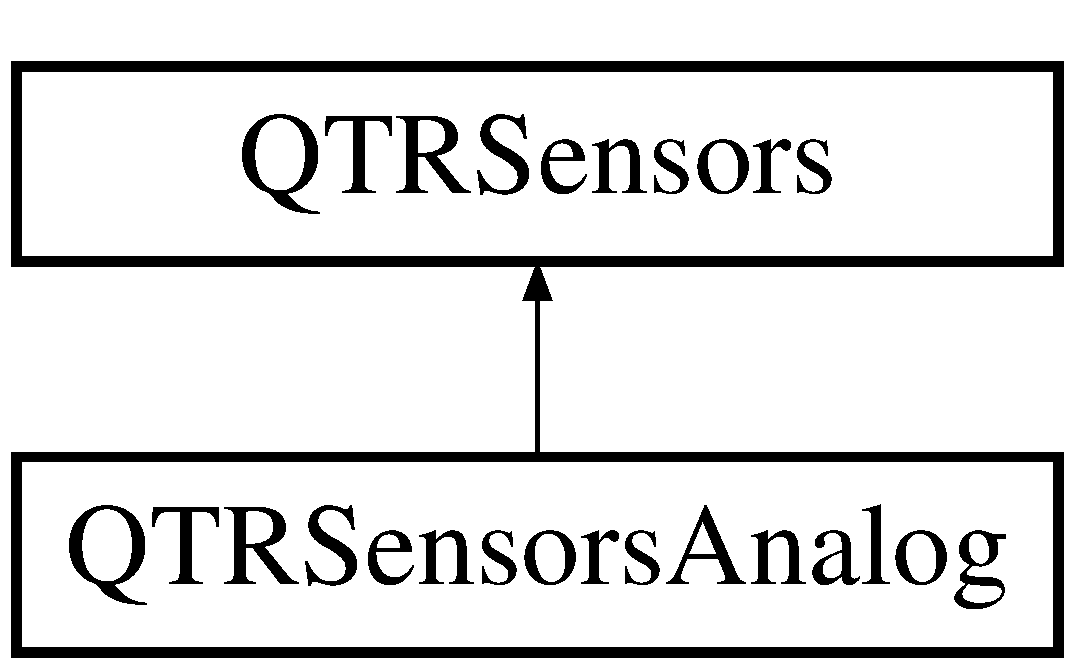
\includegraphics[height=2.000000cm]{class_q_t_r_sensors_analog}
\end{center}
\end{figure}
\doxysubsection*{Public Member Functions}
\begin{DoxyCompactItemize}
\item 
\mbox{\Hypertarget{class_q_t_r_sensors_analog_a339096d553eeae6a83e48bb8d52182f5}\label{class_q_t_r_sensors_analog_a339096d553eeae6a83e48bb8d52182f5}} 
{\bfseries QTRSensors\+Analog} (unsigned char $\ast$pins, unsigned char num\+Sensors, unsigned char num\+Samples\+Per\+Sensor=4, unsigned char emitter\+Pin=255)
\item 
\mbox{\Hypertarget{class_q_t_r_sensors_analog_a98dc112c2cf9108abf3adf2c5a8ed74d}\label{class_q_t_r_sensors_analog_a98dc112c2cf9108abf3adf2c5a8ed74d}} 
void {\bfseries init} (unsigned char $\ast$analog\+Pins, unsigned char num\+Sensors, unsigned char num\+Samples\+Per\+Sensor=4, unsigned char emitter\+Pin=QTR\+\_\+\+NO\+\_\+\+EMITTER\+\_\+\+PIN)
\item 
\mbox{\Hypertarget{class_q_t_r_sensors_afc47e6c2608293a610e1a3acce93628b}\label{class_q_t_r_sensors_afc47e6c2608293a610e1a3acce93628b}} 
void {\bfseries read} (unsigned int $\ast$sensor\+\_\+values, unsigned char read\+Mode=QTR\+\_\+\+EMITTERS\+\_\+\+ON)
\item 
\mbox{\Hypertarget{class_q_t_r_sensors_a576f1fe1e9f2d3d2097baf79a9655134}\label{class_q_t_r_sensors_a576f1fe1e9f2d3d2097baf79a9655134}} 
void {\bfseries emitters\+Off} ()
\item 
\mbox{\Hypertarget{class_q_t_r_sensors_a79f5380ecdb324a7800a045c3506975f}\label{class_q_t_r_sensors_a79f5380ecdb324a7800a045c3506975f}} 
void {\bfseries emitters\+On} ()
\item 
\mbox{\Hypertarget{class_q_t_r_sensors_ac9840e2429c7a962977057ba154c77da}\label{class_q_t_r_sensors_ac9840e2429c7a962977057ba154c77da}} 
void {\bfseries calibrate} (unsigned char read\+Mode=QTR\+\_\+\+EMITTERS\+\_\+\+ON)
\item 
\mbox{\Hypertarget{class_q_t_r_sensors_aa840b6ef17562d41edf21ddd08e0672e}\label{class_q_t_r_sensors_aa840b6ef17562d41edf21ddd08e0672e}} 
void {\bfseries reset\+Calibration} ()
\item 
\mbox{\Hypertarget{class_q_t_r_sensors_aa32a448ac03cd2a45d1f14f96ac4b739}\label{class_q_t_r_sensors_aa32a448ac03cd2a45d1f14f96ac4b739}} 
void {\bfseries read\+Calibrated} (unsigned int $\ast$sensor\+\_\+values, unsigned char read\+Mode=QTR\+\_\+\+EMITTERS\+\_\+\+ON)
\item 
\mbox{\Hypertarget{class_q_t_r_sensors_ac84f0b98bceae0b59d687ae82eb92718}\label{class_q_t_r_sensors_ac84f0b98bceae0b59d687ae82eb92718}} 
int {\bfseries read\+Line} (unsigned int $\ast$sensor\+\_\+values, unsigned char read\+Mode=QTR\+\_\+\+EMITTERS\+\_\+\+ON, unsigned char white\+\_\+line=0)
\end{DoxyCompactItemize}
\doxysubsection*{Public Attributes}
\begin{DoxyCompactItemize}
\item 
\mbox{\Hypertarget{class_q_t_r_sensors_a9308c21df0015965dceb9dd1f570f78d}\label{class_q_t_r_sensors_a9308c21df0015965dceb9dd1f570f78d}} 
unsigned int $\ast$ {\bfseries calibrated\+Minimum\+On}
\item 
\mbox{\Hypertarget{class_q_t_r_sensors_ab7a739d5bb85b17e94e825454cc63195}\label{class_q_t_r_sensors_ab7a739d5bb85b17e94e825454cc63195}} 
unsigned int $\ast$ {\bfseries calibrated\+Maximum\+On}
\item 
\mbox{\Hypertarget{class_q_t_r_sensors_af299d7e4a7900f4f3d5e567a10f4ab16}\label{class_q_t_r_sensors_af299d7e4a7900f4f3d5e567a10f4ab16}} 
unsigned int $\ast$ {\bfseries calibrated\+Minimum\+Off}
\item 
\mbox{\Hypertarget{class_q_t_r_sensors_a75af08628235c3ec5d4414a6032a016c}\label{class_q_t_r_sensors_a75af08628235c3ec5d4414a6032a016c}} 
unsigned int $\ast$ {\bfseries calibrated\+Maximum\+Off}
\end{DoxyCompactItemize}
\doxysubsection*{Protected Member Functions}
\begin{DoxyCompactItemize}
\item 
\mbox{\Hypertarget{class_q_t_r_sensors_ae1d5eb9479d4dee1977109b17aece70e}\label{class_q_t_r_sensors_ae1d5eb9479d4dee1977109b17aece70e}} 
void {\bfseries init} (unsigned char $\ast$pins, unsigned char num\+Sensors, unsigned char emitter\+Pin)
\end{DoxyCompactItemize}
\doxysubsection*{Protected Attributes}
\begin{DoxyCompactItemize}
\item 
\mbox{\Hypertarget{class_q_t_r_sensors_ad22b7f2b4778133efa1967d683e5cb46}\label{class_q_t_r_sensors_ad22b7f2b4778133efa1967d683e5cb46}} 
unsigned char $\ast$ {\bfseries \+\_\+pins}
\item 
\mbox{\Hypertarget{class_q_t_r_sensors_af4e3b5b4b9fd7acb0914a9f345e446f0}\label{class_q_t_r_sensors_af4e3b5b4b9fd7acb0914a9f345e446f0}} 
unsigned char {\bfseries \+\_\+num\+Sensors}
\item 
\mbox{\Hypertarget{class_q_t_r_sensors_a116880e22fe5e5c474e021b91e04e2ac}\label{class_q_t_r_sensors_a116880e22fe5e5c474e021b91e04e2ac}} 
unsigned char {\bfseries \+\_\+emitter\+Pin}
\item 
\mbox{\Hypertarget{class_q_t_r_sensors_a88657f1405aa7dc840f2025b53e1a4b3}\label{class_q_t_r_sensors_a88657f1405aa7dc840f2025b53e1a4b3}} 
unsigned int {\bfseries \+\_\+max\+Value}
\item 
\mbox{\Hypertarget{class_q_t_r_sensors_a9c3c8b7ac645020c77ff8198145b46b6}\label{class_q_t_r_sensors_a9c3c8b7ac645020c77ff8198145b46b6}} 
int {\bfseries \+\_\+last\+Value}
\end{DoxyCompactItemize}


\doxysubsection{Detailed Description}


Definition at line 212 of file QTRSensors.\+h.



The documentation for this class was generated from the following files\+:\begin{DoxyCompactItemize}
\item 
QTRSensors.\+h\item 
QTRSensors.\+cpp\end{DoxyCompactItemize}

\hypertarget{class_q_t_r_sensors_r_c}{}\doxysection{QTRSensors\+RC Class Reference}
\label{class_q_t_r_sensors_r_c}\index{QTRSensorsRC@{QTRSensorsRC}}
Inheritance diagram for QTRSensors\+RC\+:\begin{figure}[H]
\begin{center}
\leavevmode
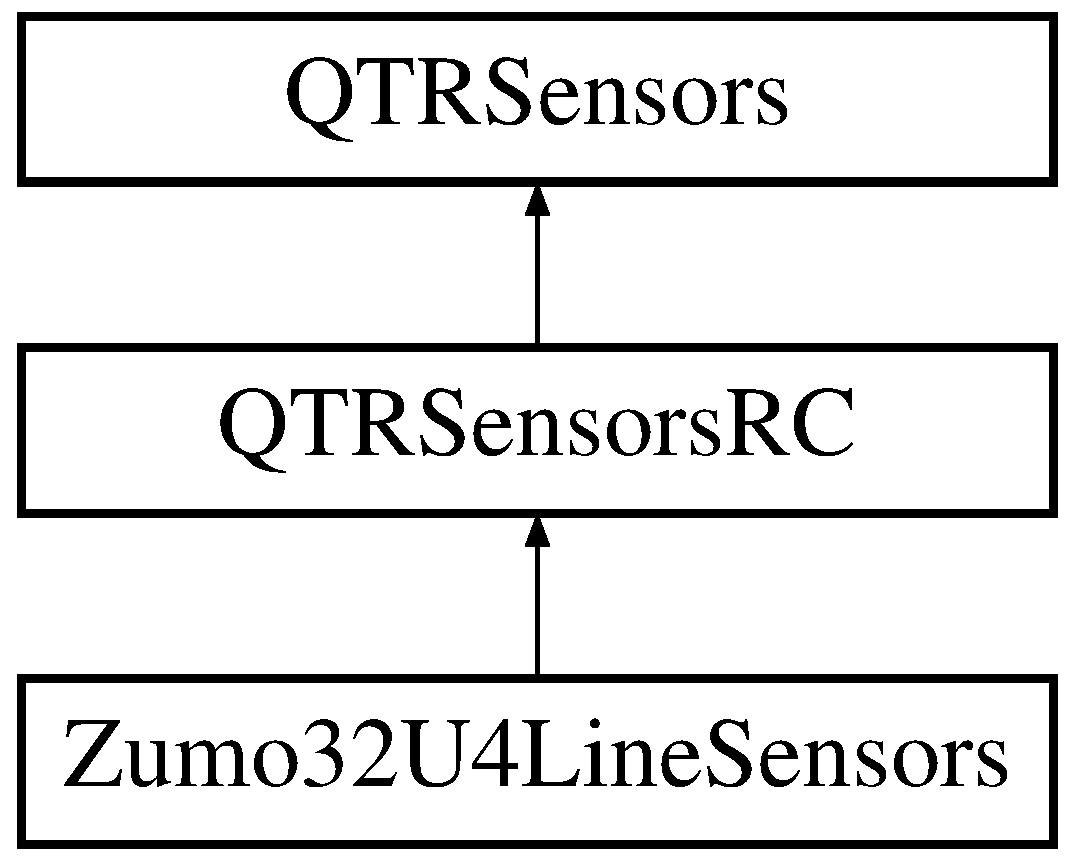
\includegraphics[height=3.000000cm]{class_q_t_r_sensors_r_c}
\end{center}
\end{figure}
\doxysubsection*{Public Member Functions}
\begin{DoxyCompactItemize}
\item 
\mbox{\hyperlink{class_q_t_r_sensors_r_c_a4e47ceb8ad4d85df3b9fe2e9f40846c9}{QTRSensors\+RC}} (unsigned char $\ast$pins, unsigned char num\+Sensors, unsigned int timeout=4000, unsigned char emitter\+Pin=255)
\item 
void \mbox{\hyperlink{class_q_t_r_sensors_r_c_a354e7064c224b6fb363405016cdf73fa}{init}} (unsigned char $\ast$pins, unsigned char num\+Sensors, unsigned int timeout=2000, unsigned char emitter\+Pin=QTR\+\_\+\+NO\+\_\+\+EMITTER\+\_\+\+PIN)
\item 
void \mbox{\hyperlink{class_q_t_r_sensors_afc47e6c2608293a610e1a3acce93628b}{read}} (unsigned int $\ast$sensor\+\_\+values, unsigned char read\+Mode=QTR\+\_\+\+EMITTERS\+\_\+\+ON)
\item 
void \mbox{\hyperlink{class_q_t_r_sensors_a576f1fe1e9f2d3d2097baf79a9655134}{emitters\+Off}} ()
\item 
void \mbox{\hyperlink{class_q_t_r_sensors_a79f5380ecdb324a7800a045c3506975f}{emitters\+On}} ()
\item 
void \mbox{\hyperlink{class_q_t_r_sensors_ac9840e2429c7a962977057ba154c77da}{calibrate}} (unsigned char read\+Mode=QTR\+\_\+\+EMITTERS\+\_\+\+ON)
\item 
void \mbox{\hyperlink{class_q_t_r_sensors_aa840b6ef17562d41edf21ddd08e0672e}{reset\+Calibration}} ()
\item 
void \mbox{\hyperlink{class_q_t_r_sensors_aa32a448ac03cd2a45d1f14f96ac4b739}{read\+Calibrated}} (unsigned int $\ast$sensor\+\_\+values, unsigned char read\+Mode=QTR\+\_\+\+EMITTERS\+\_\+\+ON)
\item 
int \mbox{\hyperlink{class_q_t_r_sensors_ac84f0b98bceae0b59d687ae82eb92718}{read\+Line}} (unsigned int $\ast$sensor\+\_\+values, unsigned char read\+Mode=QTR\+\_\+\+EMITTERS\+\_\+\+ON, unsigned char white\+\_\+line=0)
\end{DoxyCompactItemize}
\doxysubsection*{Public Attributes}
\begin{DoxyCompactItemize}
\item 
unsigned int $\ast$ \mbox{\hyperlink{class_q_t_r_sensors_a9308c21df0015965dceb9dd1f570f78d}{calibrated\+Minimum\+On}}
\item 
unsigned int $\ast$ \mbox{\hyperlink{class_q_t_r_sensors_ab7a739d5bb85b17e94e825454cc63195}{calibrated\+Maximum\+On}}
\item 
unsigned int $\ast$ \mbox{\hyperlink{class_q_t_r_sensors_af299d7e4a7900f4f3d5e567a10f4ab16}{calibrated\+Minimum\+Off}}
\item 
unsigned int $\ast$ \mbox{\hyperlink{class_q_t_r_sensors_a75af08628235c3ec5d4414a6032a016c}{calibrated\+Maximum\+Off}}
\end{DoxyCompactItemize}
\doxysubsection*{Protected Member Functions}
\begin{DoxyCompactItemize}
\item 
void \mbox{\hyperlink{class_q_t_r_sensors_ae1d5eb9479d4dee1977109b17aece70e}{init}} (unsigned char $\ast$pins, unsigned char num\+Sensors, unsigned char emitter\+Pin)
\end{DoxyCompactItemize}
\doxysubsection*{Protected Attributes}
\begin{DoxyCompactItemize}
\item 
unsigned char $\ast$ \mbox{\hyperlink{class_q_t_r_sensors_ad22b7f2b4778133efa1967d683e5cb46}{\+\_\+pins}}
\item 
unsigned char \mbox{\hyperlink{class_q_t_r_sensors_af4e3b5b4b9fd7acb0914a9f345e446f0}{\+\_\+num\+Sensors}}
\item 
unsigned char \mbox{\hyperlink{class_q_t_r_sensors_a116880e22fe5e5c474e021b91e04e2ac}{\+\_\+emitter\+Pin}}
\item 
unsigned int \mbox{\hyperlink{class_q_t_r_sensors_a88657f1405aa7dc840f2025b53e1a4b3}{\+\_\+max\+Value}}
\item 
int \mbox{\hyperlink{class_q_t_r_sensors_a9c3c8b7ac645020c77ff8198145b46b6}{\+\_\+last\+Value}}
\end{DoxyCompactItemize}


\doxysubsection{Detailed Description}


Definition at line \mbox{\hyperlink{_q_t_r_sensors_8h_source_l00161}{161}} of file \mbox{\hyperlink{_q_t_r_sensors_8h_source}{QTRSensors.\+h}}.



\doxysubsection{Constructor \& Destructor Documentation}
\mbox{\Hypertarget{class_q_t_r_sensors_r_c_a12b910f798d2eb79f1b239ca12b1dd7f}\label{class_q_t_r_sensors_r_c_a12b910f798d2eb79f1b239ca12b1dd7f}} 
\index{QTRSensorsRC@{QTRSensorsRC}!QTRSensorsRC@{QTRSensorsRC}}
\index{QTRSensorsRC@{QTRSensorsRC}!QTRSensorsRC@{QTRSensorsRC}}
\doxysubsubsection{\texorpdfstring{QTRSensorsRC()}{QTRSensorsRC()}\hspace{0.1cm}{\footnotesize\ttfamily [1/2]}}
{\footnotesize\ttfamily QTRSensors\+RC\+::\+QTRSensors\+RC (\begin{DoxyParamCaption}{ }\end{DoxyParamCaption})}



Definition at line \mbox{\hyperlink{_q_t_r_sensors_8cpp_source_l00365}{365}} of file \mbox{\hyperlink{_q_t_r_sensors_8cpp_source}{QTRSensors.\+cpp}}.

\mbox{\Hypertarget{class_q_t_r_sensors_r_c_a4e47ceb8ad4d85df3b9fe2e9f40846c9}\label{class_q_t_r_sensors_r_c_a4e47ceb8ad4d85df3b9fe2e9f40846c9}} 
\index{QTRSensorsRC@{QTRSensorsRC}!QTRSensorsRC@{QTRSensorsRC}}
\index{QTRSensorsRC@{QTRSensorsRC}!QTRSensorsRC@{QTRSensorsRC}}
\doxysubsubsection{\texorpdfstring{QTRSensorsRC()}{QTRSensorsRC()}\hspace{0.1cm}{\footnotesize\ttfamily [2/2]}}
{\footnotesize\ttfamily QTRSensors\+RC\+::\+QTRSensors\+RC (\begin{DoxyParamCaption}\item[{unsigned char $\ast$}]{pins,  }\item[{unsigned char}]{num\+Sensors,  }\item[{unsigned int}]{timeout = {\ttfamily 4000},  }\item[{unsigned char}]{emitter\+Pin = {\ttfamily 255} }\end{DoxyParamCaption})}



Definition at line \mbox{\hyperlink{_q_t_r_sensors_8cpp_source_l00374}{374}} of file \mbox{\hyperlink{_q_t_r_sensors_8cpp_source}{QTRSensors.\+cpp}}.



\doxysubsection{Member Function Documentation}
\mbox{\Hypertarget{class_q_t_r_sensors_ac9840e2429c7a962977057ba154c77da}\label{class_q_t_r_sensors_ac9840e2429c7a962977057ba154c77da}} 
\index{QTRSensorsRC@{QTRSensorsRC}!calibrate@{calibrate}}
\index{calibrate@{calibrate}!QTRSensorsRC@{QTRSensorsRC}}
\doxysubsubsection{\texorpdfstring{calibrate()}{calibrate()}}
{\footnotesize\ttfamily void QTRSensors\+::calibrate (\begin{DoxyParamCaption}\item[{unsigned char}]{read\+Mode = {\ttfamily QTR\+\_\+EMITTERS\+\_\+ON} }\end{DoxyParamCaption})\hspace{0.3cm}{\ttfamily [inherited]}}



Definition at line \mbox{\hyperlink{_q_t_r_sensors_8cpp_source_l00149}{149}} of file \mbox{\hyperlink{_q_t_r_sensors_8cpp_source}{QTRSensors.\+cpp}}.

\mbox{\Hypertarget{class_q_t_r_sensors_a576f1fe1e9f2d3d2097baf79a9655134}\label{class_q_t_r_sensors_a576f1fe1e9f2d3d2097baf79a9655134}} 
\index{QTRSensorsRC@{QTRSensorsRC}!emittersOff@{emittersOff}}
\index{emittersOff@{emittersOff}!QTRSensorsRC@{QTRSensorsRC}}
\doxysubsubsection{\texorpdfstring{emittersOff()}{emittersOff()}}
{\footnotesize\ttfamily void QTRSensors\+::emitters\+Off (\begin{DoxyParamCaption}{ }\end{DoxyParamCaption})\hspace{0.3cm}{\ttfamily [inherited]}}



Definition at line \mbox{\hyperlink{_q_t_r_sensors_8cpp_source_l00110}{110}} of file \mbox{\hyperlink{_q_t_r_sensors_8cpp_source}{QTRSensors.\+cpp}}.

\mbox{\Hypertarget{class_q_t_r_sensors_a79f5380ecdb324a7800a045c3506975f}\label{class_q_t_r_sensors_a79f5380ecdb324a7800a045c3506975f}} 
\index{QTRSensorsRC@{QTRSensorsRC}!emittersOn@{emittersOn}}
\index{emittersOn@{emittersOn}!QTRSensorsRC@{QTRSensorsRC}}
\doxysubsubsection{\texorpdfstring{emittersOn()}{emittersOn()}}
{\footnotesize\ttfamily void QTRSensors\+::emitters\+On (\begin{DoxyParamCaption}{ }\end{DoxyParamCaption})\hspace{0.3cm}{\ttfamily [inherited]}}



Definition at line \mbox{\hyperlink{_q_t_r_sensors_8cpp_source_l00119}{119}} of file \mbox{\hyperlink{_q_t_r_sensors_8cpp_source}{QTRSensors.\+cpp}}.

\mbox{\Hypertarget{class_q_t_r_sensors_ae1d5eb9479d4dee1977109b17aece70e}\label{class_q_t_r_sensors_ae1d5eb9479d4dee1977109b17aece70e}} 
\index{QTRSensorsRC@{QTRSensorsRC}!init@{init}}
\index{init@{init}!QTRSensorsRC@{QTRSensorsRC}}
\doxysubsubsection{\texorpdfstring{init()}{init()}\hspace{0.1cm}{\footnotesize\ttfamily [1/2]}}
{\footnotesize\ttfamily void QTRSensors\+::init (\begin{DoxyParamCaption}\item[{unsigned char $\ast$}]{pins,  }\item[{unsigned char}]{num\+Sensors,  }\item[{unsigned char}]{emitter\+Pin }\end{DoxyParamCaption})\hspace{0.3cm}{\ttfamily [protected]}, {\ttfamily [inherited]}}



Definition at line \mbox{\hyperlink{_q_t_r_sensors_8cpp_source_l00041}{41}} of file \mbox{\hyperlink{_q_t_r_sensors_8cpp_source}{QTRSensors.\+cpp}}.

\mbox{\Hypertarget{class_q_t_r_sensors_r_c_a354e7064c224b6fb363405016cdf73fa}\label{class_q_t_r_sensors_r_c_a354e7064c224b6fb363405016cdf73fa}} 
\index{QTRSensorsRC@{QTRSensorsRC}!init@{init}}
\index{init@{init}!QTRSensorsRC@{QTRSensorsRC}}
\doxysubsubsection{\texorpdfstring{init()}{init()}\hspace{0.1cm}{\footnotesize\ttfamily [2/2]}}
{\footnotesize\ttfamily void QTRSensors\+RC\+::init (\begin{DoxyParamCaption}\item[{unsigned char $\ast$}]{pins,  }\item[{unsigned char}]{num\+Sensors,  }\item[{unsigned int}]{timeout = {\ttfamily 2000},  }\item[{unsigned char}]{emitter\+Pin = {\ttfamily QTR\+\_\+NO\+\_\+EMITTER\+\_\+PIN} }\end{DoxyParamCaption})}



Definition at line \mbox{\hyperlink{_q_t_r_sensors_8cpp_source_l00407}{407}} of file \mbox{\hyperlink{_q_t_r_sensors_8cpp_source}{QTRSensors.\+cpp}}.

\mbox{\Hypertarget{class_q_t_r_sensors_afc47e6c2608293a610e1a3acce93628b}\label{class_q_t_r_sensors_afc47e6c2608293a610e1a3acce93628b}} 
\index{QTRSensorsRC@{QTRSensorsRC}!read@{read}}
\index{read@{read}!QTRSensorsRC@{QTRSensorsRC}}
\doxysubsubsection{\texorpdfstring{read()}{read()}}
{\footnotesize\ttfamily void QTRSensors\+::read (\begin{DoxyParamCaption}\item[{unsigned int $\ast$}]{sensor\+\_\+values,  }\item[{unsigned char}]{read\+Mode = {\ttfamily QTR\+\_\+EMITTERS\+\_\+ON} }\end{DoxyParamCaption})\hspace{0.3cm}{\ttfamily [inherited]}}



Definition at line \mbox{\hyperlink{_q_t_r_sensors_8cpp_source_l00081}{81}} of file \mbox{\hyperlink{_q_t_r_sensors_8cpp_source}{QTRSensors.\+cpp}}.

\mbox{\Hypertarget{class_q_t_r_sensors_aa32a448ac03cd2a45d1f14f96ac4b739}\label{class_q_t_r_sensors_aa32a448ac03cd2a45d1f14f96ac4b739}} 
\index{QTRSensorsRC@{QTRSensorsRC}!readCalibrated@{readCalibrated}}
\index{readCalibrated@{readCalibrated}!QTRSensorsRC@{QTRSensorsRC}}
\doxysubsubsection{\texorpdfstring{readCalibrated()}{readCalibrated()}}
{\footnotesize\ttfamily void QTRSensors\+::read\+Calibrated (\begin{DoxyParamCaption}\item[{unsigned int $\ast$}]{sensor\+\_\+values,  }\item[{unsigned char}]{read\+Mode = {\ttfamily QTR\+\_\+EMITTERS\+\_\+ON} }\end{DoxyParamCaption})\hspace{0.3cm}{\ttfamily [inherited]}}



Definition at line \mbox{\hyperlink{_q_t_r_sensors_8cpp_source_l00235}{235}} of file \mbox{\hyperlink{_q_t_r_sensors_8cpp_source}{QTRSensors.\+cpp}}.

\mbox{\Hypertarget{class_q_t_r_sensors_ac84f0b98bceae0b59d687ae82eb92718}\label{class_q_t_r_sensors_ac84f0b98bceae0b59d687ae82eb92718}} 
\index{QTRSensorsRC@{QTRSensorsRC}!readLine@{readLine}}
\index{readLine@{readLine}!QTRSensorsRC@{QTRSensorsRC}}
\doxysubsubsection{\texorpdfstring{readLine()}{readLine()}}
{\footnotesize\ttfamily int QTRSensors\+::read\+Line (\begin{DoxyParamCaption}\item[{unsigned int $\ast$}]{sensor\+\_\+values,  }\item[{unsigned char}]{read\+Mode = {\ttfamily QTR\+\_\+EMITTERS\+\_\+ON},  }\item[{unsigned char}]{white\+\_\+line = {\ttfamily 0} }\end{DoxyParamCaption})\hspace{0.3cm}{\ttfamily [inherited]}}



Definition at line \mbox{\hyperlink{_q_t_r_sensors_8cpp_source_l00315}{315}} of file \mbox{\hyperlink{_q_t_r_sensors_8cpp_source}{QTRSensors.\+cpp}}.

\mbox{\Hypertarget{class_q_t_r_sensors_aa840b6ef17562d41edf21ddd08e0672e}\label{class_q_t_r_sensors_aa840b6ef17562d41edf21ddd08e0672e}} 
\index{QTRSensorsRC@{QTRSensorsRC}!resetCalibration@{resetCalibration}}
\index{resetCalibration@{resetCalibration}!QTRSensorsRC@{QTRSensorsRC}}
\doxysubsubsection{\texorpdfstring{resetCalibration()}{resetCalibration()}}
{\footnotesize\ttfamily void QTRSensors\+::reset\+Calibration (\begin{DoxyParamCaption}{ }\end{DoxyParamCaption})\hspace{0.3cm}{\ttfamily [inherited]}}



Definition at line \mbox{\hyperlink{_q_t_r_sensors_8cpp_source_l00129}{129}} of file \mbox{\hyperlink{_q_t_r_sensors_8cpp_source}{QTRSensors.\+cpp}}.



\doxysubsection{Member Data Documentation}
\mbox{\Hypertarget{class_q_t_r_sensors_a116880e22fe5e5c474e021b91e04e2ac}\label{class_q_t_r_sensors_a116880e22fe5e5c474e021b91e04e2ac}} 
\index{QTRSensorsRC@{QTRSensorsRC}!\_emitterPin@{\_emitterPin}}
\index{\_emitterPin@{\_emitterPin}!QTRSensorsRC@{QTRSensorsRC}}
\doxysubsubsection{\texorpdfstring{\_emitterPin}{\_emitterPin}}
{\footnotesize\ttfamily unsigned char QTRSensors\+::\+\_\+emitter\+Pin\hspace{0.3cm}{\ttfamily [protected]}, {\ttfamily [inherited]}}



Definition at line \mbox{\hyperlink{_q_t_r_sensors_8h_source_l00142}{142}} of file \mbox{\hyperlink{_q_t_r_sensors_8h_source}{QTRSensors.\+h}}.

\mbox{\Hypertarget{class_q_t_r_sensors_a9c3c8b7ac645020c77ff8198145b46b6}\label{class_q_t_r_sensors_a9c3c8b7ac645020c77ff8198145b46b6}} 
\index{QTRSensorsRC@{QTRSensorsRC}!\_lastValue@{\_lastValue}}
\index{\_lastValue@{\_lastValue}!QTRSensorsRC@{QTRSensorsRC}}
\doxysubsubsection{\texorpdfstring{\_lastValue}{\_lastValue}}
{\footnotesize\ttfamily int QTRSensors\+::\+\_\+last\+Value\hspace{0.3cm}{\ttfamily [protected]}, {\ttfamily [inherited]}}



Definition at line \mbox{\hyperlink{_q_t_r_sensors_8h_source_l00144}{144}} of file \mbox{\hyperlink{_q_t_r_sensors_8h_source}{QTRSensors.\+h}}.

\mbox{\Hypertarget{class_q_t_r_sensors_a88657f1405aa7dc840f2025b53e1a4b3}\label{class_q_t_r_sensors_a88657f1405aa7dc840f2025b53e1a4b3}} 
\index{QTRSensorsRC@{QTRSensorsRC}!\_maxValue@{\_maxValue}}
\index{\_maxValue@{\_maxValue}!QTRSensorsRC@{QTRSensorsRC}}
\doxysubsubsection{\texorpdfstring{\_maxValue}{\_maxValue}}
{\footnotesize\ttfamily unsigned int QTRSensors\+::\+\_\+max\+Value\hspace{0.3cm}{\ttfamily [protected]}, {\ttfamily [inherited]}}



Definition at line \mbox{\hyperlink{_q_t_r_sensors_8h_source_l00143}{143}} of file \mbox{\hyperlink{_q_t_r_sensors_8h_source}{QTRSensors.\+h}}.

\mbox{\Hypertarget{class_q_t_r_sensors_af4e3b5b4b9fd7acb0914a9f345e446f0}\label{class_q_t_r_sensors_af4e3b5b4b9fd7acb0914a9f345e446f0}} 
\index{QTRSensorsRC@{QTRSensorsRC}!\_numSensors@{\_numSensors}}
\index{\_numSensors@{\_numSensors}!QTRSensorsRC@{QTRSensorsRC}}
\doxysubsubsection{\texorpdfstring{\_numSensors}{\_numSensors}}
{\footnotesize\ttfamily unsigned char QTRSensors\+::\+\_\+num\+Sensors\hspace{0.3cm}{\ttfamily [protected]}, {\ttfamily [inherited]}}



Definition at line \mbox{\hyperlink{_q_t_r_sensors_8h_source_l00141}{141}} of file \mbox{\hyperlink{_q_t_r_sensors_8h_source}{QTRSensors.\+h}}.

\mbox{\Hypertarget{class_q_t_r_sensors_ad22b7f2b4778133efa1967d683e5cb46}\label{class_q_t_r_sensors_ad22b7f2b4778133efa1967d683e5cb46}} 
\index{QTRSensorsRC@{QTRSensorsRC}!\_pins@{\_pins}}
\index{\_pins@{\_pins}!QTRSensorsRC@{QTRSensorsRC}}
\doxysubsubsection{\texorpdfstring{\_pins}{\_pins}}
{\footnotesize\ttfamily unsigned char$\ast$ QTRSensors\+::\+\_\+pins\hspace{0.3cm}{\ttfamily [protected]}, {\ttfamily [inherited]}}



Definition at line \mbox{\hyperlink{_q_t_r_sensors_8h_source_l00140}{140}} of file \mbox{\hyperlink{_q_t_r_sensors_8h_source}{QTRSensors.\+h}}.

\mbox{\Hypertarget{class_q_t_r_sensors_a75af08628235c3ec5d4414a6032a016c}\label{class_q_t_r_sensors_a75af08628235c3ec5d4414a6032a016c}} 
\index{QTRSensorsRC@{QTRSensorsRC}!calibratedMaximumOff@{calibratedMaximumOff}}
\index{calibratedMaximumOff@{calibratedMaximumOff}!QTRSensorsRC@{QTRSensorsRC}}
\doxysubsubsection{\texorpdfstring{calibratedMaximumOff}{calibratedMaximumOff}}
{\footnotesize\ttfamily unsigned int$\ast$ QTRSensors\+::calibrated\+Maximum\+Off\hspace{0.3cm}{\ttfamily [inherited]}}



Definition at line \mbox{\hyperlink{_q_t_r_sensors_8h_source_l00127}{127}} of file \mbox{\hyperlink{_q_t_r_sensors_8h_source}{QTRSensors.\+h}}.

\mbox{\Hypertarget{class_q_t_r_sensors_ab7a739d5bb85b17e94e825454cc63195}\label{class_q_t_r_sensors_ab7a739d5bb85b17e94e825454cc63195}} 
\index{QTRSensorsRC@{QTRSensorsRC}!calibratedMaximumOn@{calibratedMaximumOn}}
\index{calibratedMaximumOn@{calibratedMaximumOn}!QTRSensorsRC@{QTRSensorsRC}}
\doxysubsubsection{\texorpdfstring{calibratedMaximumOn}{calibratedMaximumOn}}
{\footnotesize\ttfamily unsigned int$\ast$ QTRSensors\+::calibrated\+Maximum\+On\hspace{0.3cm}{\ttfamily [inherited]}}



Definition at line \mbox{\hyperlink{_q_t_r_sensors_8h_source_l00125}{125}} of file \mbox{\hyperlink{_q_t_r_sensors_8h_source}{QTRSensors.\+h}}.

\mbox{\Hypertarget{class_q_t_r_sensors_af299d7e4a7900f4f3d5e567a10f4ab16}\label{class_q_t_r_sensors_af299d7e4a7900f4f3d5e567a10f4ab16}} 
\index{QTRSensorsRC@{QTRSensorsRC}!calibratedMinimumOff@{calibratedMinimumOff}}
\index{calibratedMinimumOff@{calibratedMinimumOff}!QTRSensorsRC@{QTRSensorsRC}}
\doxysubsubsection{\texorpdfstring{calibratedMinimumOff}{calibratedMinimumOff}}
{\footnotesize\ttfamily unsigned int$\ast$ QTRSensors\+::calibrated\+Minimum\+Off\hspace{0.3cm}{\ttfamily [inherited]}}



Definition at line \mbox{\hyperlink{_q_t_r_sensors_8h_source_l00126}{126}} of file \mbox{\hyperlink{_q_t_r_sensors_8h_source}{QTRSensors.\+h}}.

\mbox{\Hypertarget{class_q_t_r_sensors_a9308c21df0015965dceb9dd1f570f78d}\label{class_q_t_r_sensors_a9308c21df0015965dceb9dd1f570f78d}} 
\index{QTRSensorsRC@{QTRSensorsRC}!calibratedMinimumOn@{calibratedMinimumOn}}
\index{calibratedMinimumOn@{calibratedMinimumOn}!QTRSensorsRC@{QTRSensorsRC}}
\doxysubsubsection{\texorpdfstring{calibratedMinimumOn}{calibratedMinimumOn}}
{\footnotesize\ttfamily unsigned int$\ast$ QTRSensors\+::calibrated\+Minimum\+On\hspace{0.3cm}{\ttfamily [inherited]}}



Definition at line \mbox{\hyperlink{_q_t_r_sensors_8h_source_l00124}{124}} of file \mbox{\hyperlink{_q_t_r_sensors_8h_source}{QTRSensors.\+h}}.



The documentation for this class was generated from the following files\+:\begin{DoxyCompactItemize}
\item 
QTRSensors.\+h\item 
QTRSensors.\+cpp\end{DoxyCompactItemize}

\hypertarget{class_u_s_b_pause}{}\doxysection{USBPause Class Reference}
\label{class_u_s_b_pause}\index{USBPause@{USBPause}}


{\ttfamily \#include $<$USBPause.\+h$>$}



\doxysubsection{Detailed Description}
This class disables USB interrupts in its constructor when it is created and restores them to their previous state in its destructor when it is destroyed. This class is tailored to the behavior of the Arduino core USB code, so it might have to change if that code changes.

This class assumes that the only USB interrupts enabled are general device interrupts and endpoint 0 interrupts.

It also assumes that the endpoint 0 interrupts will not enable or disable any of the general device interrupts. 

Definition at line \mbox{\hyperlink{_u_s_b_pause_8h_source_l00026}{26}} of file \mbox{\hyperlink{_u_s_b_pause_8h_source}{USBPause.\+h}}.



\doxysubsection{Constructor \& Destructor Documentation}
\mbox{\Hypertarget{class_u_s_b_pause_a8e4272630d20cd851843c504b1f75c0b}\label{class_u_s_b_pause_a8e4272630d20cd851843c504b1f75c0b}} 
\index{USBPause@{USBPause}!USBPause@{USBPause}}
\index{USBPause@{USBPause}!USBPause@{USBPause}}
\doxysubsubsection{\texorpdfstring{USBPause()}{USBPause()}}
{\footnotesize\ttfamily USBPause\+::\+USBPause (\begin{DoxyParamCaption}{ }\end{DoxyParamCaption})\hspace{0.3cm}{\ttfamily [inline]}}



Definition at line \mbox{\hyperlink{_u_s_b_pause_8h_source_l00039}{39}} of file \mbox{\hyperlink{_u_s_b_pause_8h_source}{USBPause.\+h}}.

\mbox{\Hypertarget{class_u_s_b_pause_afaa942011cec42c76dbca489a3b36a59}\label{class_u_s_b_pause_afaa942011cec42c76dbca489a3b36a59}} 
\index{USBPause@{USBPause}!````~USBPause@{$\sim$USBPause}}
\index{````~USBPause@{$\sim$USBPause}!USBPause@{USBPause}}
\doxysubsubsection{\texorpdfstring{$\sim$USBPause()}{~USBPause()}}
{\footnotesize\ttfamily USBPause\+::$\sim$\+USBPause (\begin{DoxyParamCaption}{ }\end{DoxyParamCaption})\hspace{0.3cm}{\ttfamily [inline]}}



Definition at line \mbox{\hyperlink{_u_s_b_pause_8h_source_l00056}{56}} of file \mbox{\hyperlink{_u_s_b_pause_8h_source}{USBPause.\+h}}.



The documentation for this class was generated from the following file\+:\begin{DoxyCompactItemize}
\item 
\mbox{\hyperlink{_u_s_b_pause_8h}{USBPause.\+h}}\end{DoxyCompactItemize}

\hypertarget{struct_zumo32_u4_i_m_u_1_1vector}{}\doxysection{Zumo32\+U4\+IMU\+::vector$<$ T $>$ Struct Template Reference}
\label{struct_zumo32_u4_i_m_u_1_1vector}\index{Zumo32U4IMU::vector$<$ T $>$@{Zumo32U4IMU::vector$<$ T $>$}}


Represents a 3-\/dimensional vector with x, y, and z components.  




{\ttfamily \#include $<$Zumo32\+U4\+IMU.\+h$>$}

\doxysubsection*{Public Attributes}
\begin{DoxyCompactItemize}
\item 
\mbox{\Hypertarget{struct_zumo32_u4_i_m_u_1_1vector_a5e37cb6956780f070644342cfd3a3445}\label{struct_zumo32_u4_i_m_u_1_1vector_a5e37cb6956780f070644342cfd3a3445}} 
T {\bfseries x}
\item 
\mbox{\Hypertarget{struct_zumo32_u4_i_m_u_1_1vector_a17f578bba75257eb6a424d5df4a3ac37}\label{struct_zumo32_u4_i_m_u_1_1vector_a17f578bba75257eb6a424d5df4a3ac37}} 
T {\bfseries y}
\item 
\mbox{\Hypertarget{struct_zumo32_u4_i_m_u_1_1vector_adabd262931612a0909326f4292982874}\label{struct_zumo32_u4_i_m_u_1_1vector_adabd262931612a0909326f4292982874}} 
T {\bfseries z}
\end{DoxyCompactItemize}


\doxysubsection{Detailed Description}
\subsubsection*{template$<$typename T$>$\newline
struct Zumo32\+U4\+IMU\+::vector$<$ T $>$}

Represents a 3-\/dimensional vector with x, y, and z components. 

Definition at line 81 of file Zumo32\+U4\+IMU.\+h.



The documentation for this struct was generated from the following file\+:\begin{DoxyCompactItemize}
\item 
\mbox{\hyperlink{_zumo32_u4_i_m_u_8h}{Zumo32\+U4\+IMU.\+h}}\end{DoxyCompactItemize}

\hypertarget{class_zumo32_u4_button_a}{}\doxysection{Zumo32\+U4\+ButtonA Class Reference}
\label{class_zumo32_u4_button_a}\index{Zumo32U4ButtonA@{Zumo32U4ButtonA}}


Interfaces with button A on the Zumo 32U4.  




{\ttfamily \#include $<$Zumo32\+U4\+Buttons.\+h$>$}

Inheritance diagram for Zumo32\+U4\+ButtonA\+:\begin{figure}[H]
\begin{center}
\leavevmode
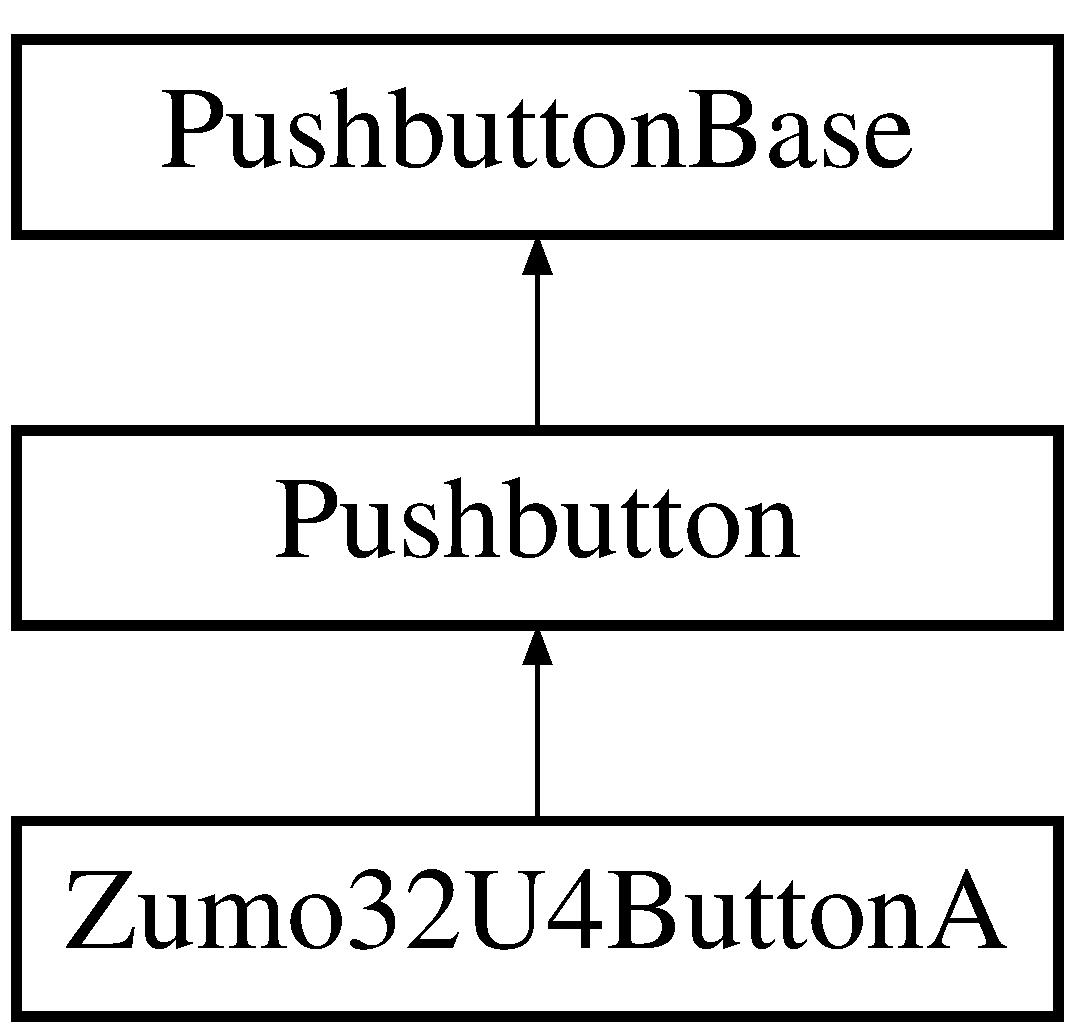
\includegraphics[height=3.000000cm]{class_zumo32_u4_button_a}
\end{center}
\end{figure}
\doxysubsection*{Public Member Functions}
\begin{DoxyCompactItemize}
\item 
virtual bool \mbox{\hyperlink{class_pushbutton_a4990786220489fb5b6cf3af19b601a24}{is\+Pressed}} ()
\begin{DoxyCompactList}\small\item\em indicates whether button is currently pressed without any debouncing. \end{DoxyCompactList}\item 
void \mbox{\hyperlink{class_pushbutton_base_a2e2787595c82ee0913ecf4c1eea4a2c8}{wait\+For\+Press}} ()
\begin{DoxyCompactList}\small\item\em Waits until the button is pressed and takes care of debouncing. \end{DoxyCompactList}\item 
void \mbox{\hyperlink{class_pushbutton_base_ae5fff34b3e1ebd62fd02b99edd6bf13a}{wait\+For\+Release}} ()
\begin{DoxyCompactList}\small\item\em Waits until the button is released and takes care of debouncing. \end{DoxyCompactList}\item 
void \mbox{\hyperlink{class_pushbutton_base_ab755065c930be0649597220316213e8a}{wait\+For\+Button}} ()
\begin{DoxyCompactList}\small\item\em Waits until the button is pressed and then waits until the button is released, taking care of debouncing. \end{DoxyCompactList}\item 
bool \mbox{\hyperlink{class_pushbutton_base_a93953875c8b1c5f69dec3984774de296}{get\+Single\+Debounced\+Press}} ()
\begin{DoxyCompactList}\small\item\em Uses a state machine to return true once after each time it detects the button moving from the released state to the pressed state. \end{DoxyCompactList}\item 
bool \mbox{\hyperlink{class_pushbutton_base_ae568f5db0e8804247e0dcab72a311d42}{get\+Single\+Debounced\+Release}} ()
\begin{DoxyCompactList}\small\item\em Uses a state machine to return true once after each time it detects the button moving from the pressed state to the released state. \end{DoxyCompactList}\end{DoxyCompactItemize}


\doxysubsection{Detailed Description}
Interfaces with button A on the Zumo 32U4. 

Definition at line 24 of file Zumo32\+U4\+Buttons.\+h.



\doxysubsection{Member Function Documentation}
\mbox{\Hypertarget{class_pushbutton_base_a93953875c8b1c5f69dec3984774de296}\label{class_pushbutton_base_a93953875c8b1c5f69dec3984774de296}} 
\index{Zumo32U4ButtonA@{Zumo32U4ButtonA}!getSingleDebouncedPress@{getSingleDebouncedPress}}
\index{getSingleDebouncedPress@{getSingleDebouncedPress}!Zumo32U4ButtonA@{Zumo32U4ButtonA}}
\doxysubsubsection{\texorpdfstring{getSingleDebouncedPress()}{getSingleDebouncedPress()}}
{\footnotesize\ttfamily bool Pushbutton\+Base\+::get\+Single\+Debounced\+Press (\begin{DoxyParamCaption}{ }\end{DoxyParamCaption})\hspace{0.3cm}{\ttfamily [inherited]}}



Uses a state machine to return true once after each time it detects the button moving from the released state to the pressed state. 

This is a non-\/blocking function that is meant to be called repeatedly in a loop. Each time it is called, it updates a state machine that monitors the state of the button. When it detects the button changing from the released state to the pressed state, with debouncing, it returns true. 

Definition at line 110 of file Pushbutton.\+cpp.

\mbox{\Hypertarget{class_pushbutton_base_ae568f5db0e8804247e0dcab72a311d42}\label{class_pushbutton_base_ae568f5db0e8804247e0dcab72a311d42}} 
\index{Zumo32U4ButtonA@{Zumo32U4ButtonA}!getSingleDebouncedRelease@{getSingleDebouncedRelease}}
\index{getSingleDebouncedRelease@{getSingleDebouncedRelease}!Zumo32U4ButtonA@{Zumo32U4ButtonA}}
\doxysubsubsection{\texorpdfstring{getSingleDebouncedRelease()}{getSingleDebouncedRelease()}}
{\footnotesize\ttfamily bool Pushbutton\+Base\+::get\+Single\+Debounced\+Release (\begin{DoxyParamCaption}{ }\end{DoxyParamCaption})\hspace{0.3cm}{\ttfamily [inherited]}}



Uses a state machine to return true once after each time it detects the button moving from the pressed state to the released state. 

This is just like \mbox{\hyperlink{class_pushbutton_base_a93953875c8b1c5f69dec3984774de296}{get\+Single\+Debounced\+Press()}} except it has a separate state machine and it watches for when the button goes from the pressed state to the released state.

There is no strict guarantee that every debounced button press event returned by \mbox{\hyperlink{class_pushbutton_base_a93953875c8b1c5f69dec3984774de296}{get\+Single\+Debounced\+Press()}} will have a corresponding button release event returned by \mbox{\hyperlink{class_pushbutton_base_ae568f5db0e8804247e0dcab72a311d42}{get\+Single\+Debounced\+Release()}}; the two functions use independent state machines and sample the button at different times. 

Definition at line 115 of file Pushbutton.\+cpp.

\mbox{\Hypertarget{class_pushbutton_a4990786220489fb5b6cf3af19b601a24}\label{class_pushbutton_a4990786220489fb5b6cf3af19b601a24}} 
\index{Zumo32U4ButtonA@{Zumo32U4ButtonA}!isPressed@{isPressed}}
\index{isPressed@{isPressed}!Zumo32U4ButtonA@{Zumo32U4ButtonA}}
\doxysubsubsection{\texorpdfstring{isPressed()}{isPressed()}}
{\footnotesize\ttfamily bool Pushbutton\+::is\+Pressed (\begin{DoxyParamCaption}{ }\end{DoxyParamCaption})\hspace{0.3cm}{\ttfamily [virtual]}, {\ttfamily [inherited]}}



indicates whether button is currently pressed without any debouncing. 

\begin{DoxyReturn}{Returns}
1 if the button is pressed right now, 0 if it is not.
\end{DoxyReturn}
This function must be implemented in a subclass of \mbox{\hyperlink{class_pushbutton_base}{Pushbutton\+Base}}, such as \mbox{\hyperlink{class_pushbutton}{Pushbutton}}. 

Implements \mbox{\hyperlink{class_pushbutton_base_a5b11851f15413140b75e4574e773b6ae}{Pushbutton\+Base}}.



Definition at line 142 of file Pushbutton.\+cpp.

\mbox{\Hypertarget{class_pushbutton_base_ab755065c930be0649597220316213e8a}\label{class_pushbutton_base_ab755065c930be0649597220316213e8a}} 
\index{Zumo32U4ButtonA@{Zumo32U4ButtonA}!waitForButton@{waitForButton}}
\index{waitForButton@{waitForButton}!Zumo32U4ButtonA@{Zumo32U4ButtonA}}
\doxysubsubsection{\texorpdfstring{waitForButton()}{waitForButton()}}
{\footnotesize\ttfamily void Pushbutton\+Base\+::wait\+For\+Button (\begin{DoxyParamCaption}{ }\end{DoxyParamCaption})\hspace{0.3cm}{\ttfamily [inherited]}}



Waits until the button is pressed and then waits until the button is released, taking care of debouncing. 

This is equivalent to calling \mbox{\hyperlink{class_pushbutton_base_a2e2787595c82ee0913ecf4c1eea4a2c8}{wait\+For\+Press()}} and then \mbox{\hyperlink{class_pushbutton_base_ae5fff34b3e1ebd62fd02b99edd6bf13a}{wait\+For\+Release()}}. 

Definition at line 104 of file Pushbutton.\+cpp.

\mbox{\Hypertarget{class_pushbutton_base_a2e2787595c82ee0913ecf4c1eea4a2c8}\label{class_pushbutton_base_a2e2787595c82ee0913ecf4c1eea4a2c8}} 
\index{Zumo32U4ButtonA@{Zumo32U4ButtonA}!waitForPress@{waitForPress}}
\index{waitForPress@{waitForPress}!Zumo32U4ButtonA@{Zumo32U4ButtonA}}
\doxysubsubsection{\texorpdfstring{waitForPress()}{waitForPress()}}
{\footnotesize\ttfamily void Pushbutton\+Base\+::wait\+For\+Press (\begin{DoxyParamCaption}{ }\end{DoxyParamCaption})\hspace{0.3cm}{\ttfamily [inherited]}}



Waits until the button is pressed and takes care of debouncing. 

This function waits until the button is in the pressed state and then returns. Note that if the button is already pressed when you call this function, it will return quickly (in 10 ms). 

Definition at line 84 of file Pushbutton.\+cpp.

\mbox{\Hypertarget{class_pushbutton_base_ae5fff34b3e1ebd62fd02b99edd6bf13a}\label{class_pushbutton_base_ae5fff34b3e1ebd62fd02b99edd6bf13a}} 
\index{Zumo32U4ButtonA@{Zumo32U4ButtonA}!waitForRelease@{waitForRelease}}
\index{waitForRelease@{waitForRelease}!Zumo32U4ButtonA@{Zumo32U4ButtonA}}
\doxysubsubsection{\texorpdfstring{waitForRelease()}{waitForRelease()}}
{\footnotesize\ttfamily void Pushbutton\+Base\+::wait\+For\+Release (\begin{DoxyParamCaption}{ }\end{DoxyParamCaption})\hspace{0.3cm}{\ttfamily [inherited]}}



Waits until the button is released and takes care of debouncing. 

This function waits until the button is in the released state and then returns. Note that if the button is already released when you call this function, it will return quickly (in 10 ms). 

Definition at line 94 of file Pushbutton.\+cpp.



The documentation for this class was generated from the following file\+:\begin{DoxyCompactItemize}
\item 
\mbox{\hyperlink{_zumo32_u4_buttons_8h}{Zumo32\+U4\+Buttons.\+h}}\end{DoxyCompactItemize}

\hypertarget{class_zumo32_u4_button_b}{}\doxysection{Zumo32\+U4\+ButtonB Class Reference}
\label{class_zumo32_u4_button_b}\index{Zumo32U4ButtonB@{Zumo32U4ButtonB}}


Interfaces with button B on the Zumo 32U4.  




{\ttfamily \#include $<$Zumo32\+U4\+Buttons.\+h$>$}

Inheritance diagram for Zumo32\+U4\+ButtonB\+:\begin{figure}[H]
\begin{center}
\leavevmode
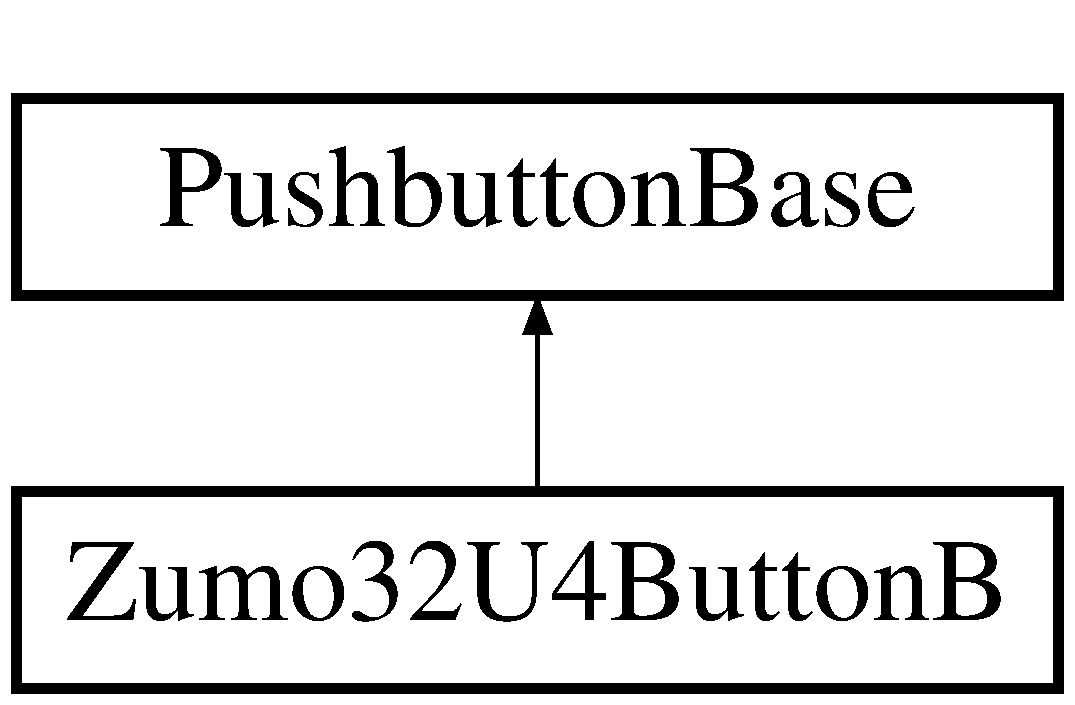
\includegraphics[height=2.000000cm]{class_zumo32_u4_button_b}
\end{center}
\end{figure}
\doxysubsection*{Public Member Functions}
\begin{DoxyCompactItemize}
\item 
virtual bool \mbox{\hyperlink{class_zumo32_u4_button_b_a013a2c0029356aece18b93963373a736}{is\+Pressed}} ()
\begin{DoxyCompactList}\small\item\em indicates whether button is currently pressed without any debouncing. \end{DoxyCompactList}\item 
void \mbox{\hyperlink{class_pushbutton_base_a2e2787595c82ee0913ecf4c1eea4a2c8}{wait\+For\+Press}} ()
\begin{DoxyCompactList}\small\item\em Waits until the button is pressed and takes care of debouncing. \end{DoxyCompactList}\item 
void \mbox{\hyperlink{class_pushbutton_base_ae5fff34b3e1ebd62fd02b99edd6bf13a}{wait\+For\+Release}} ()
\begin{DoxyCompactList}\small\item\em Waits until the button is released and takes care of debouncing. \end{DoxyCompactList}\item 
void \mbox{\hyperlink{class_pushbutton_base_ab755065c930be0649597220316213e8a}{wait\+For\+Button}} ()
\begin{DoxyCompactList}\small\item\em Waits until the button is pressed and then waits until the button is released, taking care of debouncing. \end{DoxyCompactList}\item 
bool \mbox{\hyperlink{class_pushbutton_base_a93953875c8b1c5f69dec3984774de296}{get\+Single\+Debounced\+Press}} ()
\begin{DoxyCompactList}\small\item\em Uses a state machine to return true once after each time it detects the button moving from the released state to the pressed state. \end{DoxyCompactList}\item 
bool \mbox{\hyperlink{class_pushbutton_base_ae568f5db0e8804247e0dcab72a311d42}{get\+Single\+Debounced\+Release}} ()
\begin{DoxyCompactList}\small\item\em Uses a state machine to return true once after each time it detects the button moving from the pressed state to the released state. \end{DoxyCompactList}\end{DoxyCompactItemize}


\doxysubsection{Detailed Description}
Interfaces with button B on the Zumo 32U4. 

The pin used for button B is also used for the TX LED.

This class temporarily disables USB interrupts because the Arduino core code has USB interrupts enabled that sometimes write to the pin this button is on.

This class temporarily sets the pin to be an input without a pull-\/up resistor. The pull-\/up resistor is not needed because of the resistors on the board. 

Definition at line 42 of file Zumo32\+U4\+Buttons.\+h.



\doxysubsection{Member Function Documentation}
\mbox{\Hypertarget{class_pushbutton_base_a93953875c8b1c5f69dec3984774de296}\label{class_pushbutton_base_a93953875c8b1c5f69dec3984774de296}} 
\index{Zumo32U4ButtonB@{Zumo32U4ButtonB}!getSingleDebouncedPress@{getSingleDebouncedPress}}
\index{getSingleDebouncedPress@{getSingleDebouncedPress}!Zumo32U4ButtonB@{Zumo32U4ButtonB}}
\doxysubsubsection{\texorpdfstring{getSingleDebouncedPress()}{getSingleDebouncedPress()}}
{\footnotesize\ttfamily bool Pushbutton\+Base\+::get\+Single\+Debounced\+Press (\begin{DoxyParamCaption}{ }\end{DoxyParamCaption})\hspace{0.3cm}{\ttfamily [inherited]}}



Uses a state machine to return true once after each time it detects the button moving from the released state to the pressed state. 

This is a non-\/blocking function that is meant to be called repeatedly in a loop. Each time it is called, it updates a state machine that monitors the state of the button. When it detects the button changing from the released state to the pressed state, with debouncing, it returns true. 

Definition at line 110 of file Pushbutton.\+cpp.

\mbox{\Hypertarget{class_pushbutton_base_ae568f5db0e8804247e0dcab72a311d42}\label{class_pushbutton_base_ae568f5db0e8804247e0dcab72a311d42}} 
\index{Zumo32U4ButtonB@{Zumo32U4ButtonB}!getSingleDebouncedRelease@{getSingleDebouncedRelease}}
\index{getSingleDebouncedRelease@{getSingleDebouncedRelease}!Zumo32U4ButtonB@{Zumo32U4ButtonB}}
\doxysubsubsection{\texorpdfstring{getSingleDebouncedRelease()}{getSingleDebouncedRelease()}}
{\footnotesize\ttfamily bool Pushbutton\+Base\+::get\+Single\+Debounced\+Release (\begin{DoxyParamCaption}{ }\end{DoxyParamCaption})\hspace{0.3cm}{\ttfamily [inherited]}}



Uses a state machine to return true once after each time it detects the button moving from the pressed state to the released state. 

This is just like \mbox{\hyperlink{class_pushbutton_base_a93953875c8b1c5f69dec3984774de296}{get\+Single\+Debounced\+Press()}} except it has a separate state machine and it watches for when the button goes from the pressed state to the released state.

There is no strict guarantee that every debounced button press event returned by \mbox{\hyperlink{class_pushbutton_base_a93953875c8b1c5f69dec3984774de296}{get\+Single\+Debounced\+Press()}} will have a corresponding button release event returned by \mbox{\hyperlink{class_pushbutton_base_ae568f5db0e8804247e0dcab72a311d42}{get\+Single\+Debounced\+Release()}}; the two functions use independent state machines and sample the button at different times. 

Definition at line 115 of file Pushbutton.\+cpp.

\mbox{\Hypertarget{class_zumo32_u4_button_b_a013a2c0029356aece18b93963373a736}\label{class_zumo32_u4_button_b_a013a2c0029356aece18b93963373a736}} 
\index{Zumo32U4ButtonB@{Zumo32U4ButtonB}!isPressed@{isPressed}}
\index{isPressed@{isPressed}!Zumo32U4ButtonB@{Zumo32U4ButtonB}}
\doxysubsubsection{\texorpdfstring{isPressed()}{isPressed()}}
{\footnotesize\ttfamily virtual bool Zumo32\+U4\+Button\+B\+::is\+Pressed (\begin{DoxyParamCaption}{ }\end{DoxyParamCaption})\hspace{0.3cm}{\ttfamily [inline]}, {\ttfamily [virtual]}}



indicates whether button is currently pressed without any debouncing. 

\begin{DoxyReturn}{Returns}
1 if the button is pressed right now, 0 if it is not.
\end{DoxyReturn}
This function must be implemented in a subclass of \mbox{\hyperlink{class_pushbutton_base}{Pushbutton\+Base}}, such as \mbox{\hyperlink{class_pushbutton}{Pushbutton}}. 

Implements \mbox{\hyperlink{class_pushbutton_base_a5b11851f15413140b75e4574e773b6ae}{Pushbutton\+Base}}.



Definition at line 46 of file Zumo32\+U4\+Buttons.\+h.

\mbox{\Hypertarget{class_pushbutton_base_ab755065c930be0649597220316213e8a}\label{class_pushbutton_base_ab755065c930be0649597220316213e8a}} 
\index{Zumo32U4ButtonB@{Zumo32U4ButtonB}!waitForButton@{waitForButton}}
\index{waitForButton@{waitForButton}!Zumo32U4ButtonB@{Zumo32U4ButtonB}}
\doxysubsubsection{\texorpdfstring{waitForButton()}{waitForButton()}}
{\footnotesize\ttfamily void Pushbutton\+Base\+::wait\+For\+Button (\begin{DoxyParamCaption}{ }\end{DoxyParamCaption})\hspace{0.3cm}{\ttfamily [inherited]}}



Waits until the button is pressed and then waits until the button is released, taking care of debouncing. 

This is equivalent to calling \mbox{\hyperlink{class_pushbutton_base_a2e2787595c82ee0913ecf4c1eea4a2c8}{wait\+For\+Press()}} and then \mbox{\hyperlink{class_pushbutton_base_ae5fff34b3e1ebd62fd02b99edd6bf13a}{wait\+For\+Release()}}. 

Definition at line 104 of file Pushbutton.\+cpp.

\mbox{\Hypertarget{class_pushbutton_base_a2e2787595c82ee0913ecf4c1eea4a2c8}\label{class_pushbutton_base_a2e2787595c82ee0913ecf4c1eea4a2c8}} 
\index{Zumo32U4ButtonB@{Zumo32U4ButtonB}!waitForPress@{waitForPress}}
\index{waitForPress@{waitForPress}!Zumo32U4ButtonB@{Zumo32U4ButtonB}}
\doxysubsubsection{\texorpdfstring{waitForPress()}{waitForPress()}}
{\footnotesize\ttfamily void Pushbutton\+Base\+::wait\+For\+Press (\begin{DoxyParamCaption}{ }\end{DoxyParamCaption})\hspace{0.3cm}{\ttfamily [inherited]}}



Waits until the button is pressed and takes care of debouncing. 

This function waits until the button is in the pressed state and then returns. Note that if the button is already pressed when you call this function, it will return quickly (in 10 ms). 

Definition at line 84 of file Pushbutton.\+cpp.

\mbox{\Hypertarget{class_pushbutton_base_ae5fff34b3e1ebd62fd02b99edd6bf13a}\label{class_pushbutton_base_ae5fff34b3e1ebd62fd02b99edd6bf13a}} 
\index{Zumo32U4ButtonB@{Zumo32U4ButtonB}!waitForRelease@{waitForRelease}}
\index{waitForRelease@{waitForRelease}!Zumo32U4ButtonB@{Zumo32U4ButtonB}}
\doxysubsubsection{\texorpdfstring{waitForRelease()}{waitForRelease()}}
{\footnotesize\ttfamily void Pushbutton\+Base\+::wait\+For\+Release (\begin{DoxyParamCaption}{ }\end{DoxyParamCaption})\hspace{0.3cm}{\ttfamily [inherited]}}



Waits until the button is released and takes care of debouncing. 

This function waits until the button is in the released state and then returns. Note that if the button is already released when you call this function, it will return quickly (in 10 ms). 

Definition at line 94 of file Pushbutton.\+cpp.



The documentation for this class was generated from the following file\+:\begin{DoxyCompactItemize}
\item 
\mbox{\hyperlink{_zumo32_u4_buttons_8h}{Zumo32\+U4\+Buttons.\+h}}\end{DoxyCompactItemize}

\hypertarget{class_zumo32_u4_button_c}{}\section{Zumo32\+U4\+ButtonC Class Reference}
\label{class_zumo32_u4_button_c}\index{Zumo32\+U4\+ButtonC@{Zumo32\+U4\+ButtonC}}


Interfaces with button C on the Zumo 32\+U4.  




{\ttfamily \#include $<$Zumo32\+U4\+Buttons.\+h$>$}

Inheritance diagram for Zumo32\+U4\+ButtonC\+:\begin{figure}[H]
\begin{center}
\leavevmode
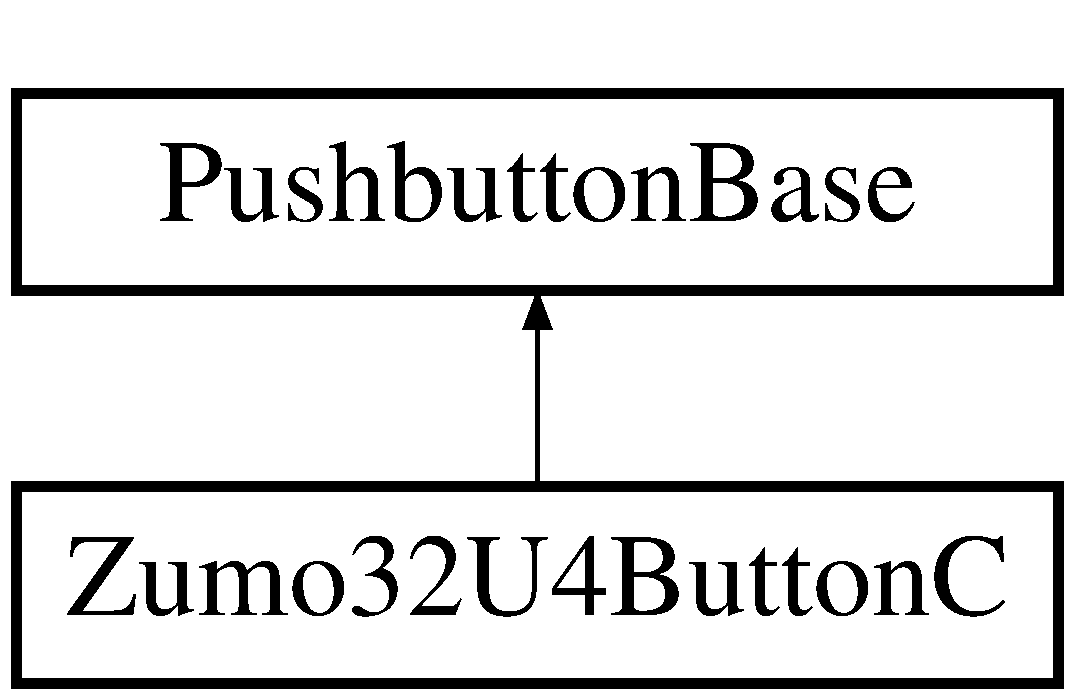
\includegraphics[height=2.000000cm]{class_zumo32_u4_button_c}
\end{center}
\end{figure}
\subsection*{Public Member Functions}
\begin{DoxyCompactItemize}
\item 
virtual bool \hyperlink{class_zumo32_u4_button_c_aa75e220cde340487a3fa8f1f99d645f8}{is\+Pressed} ()
\begin{DoxyCompactList}\small\item\em indicates whether button is currently pressed without any debouncing. \end{DoxyCompactList}\item 
void \hyperlink{class_pushbutton_base_a2e2787595c82ee0913ecf4c1eea4a2c8}{wait\+For\+Press} ()
\begin{DoxyCompactList}\small\item\em Waits until the button is pressed and takes care of debouncing. \end{DoxyCompactList}\item 
void \hyperlink{class_pushbutton_base_ae5fff34b3e1ebd62fd02b99edd6bf13a}{wait\+For\+Release} ()
\begin{DoxyCompactList}\small\item\em Waits until the button is released and takes care of debouncing. \end{DoxyCompactList}\item 
void \hyperlink{class_pushbutton_base_ab755065c930be0649597220316213e8a}{wait\+For\+Button} ()
\begin{DoxyCompactList}\small\item\em Waits until the button is pressed and then waits until the button is released, taking care of debouncing. \end{DoxyCompactList}\item 
bool \hyperlink{class_pushbutton_base_a93953875c8b1c5f69dec3984774de296}{get\+Single\+Debounced\+Press} ()
\begin{DoxyCompactList}\small\item\em Uses a state machine to return true once after each time it detects the button moving from the released state to the pressed state. \end{DoxyCompactList}\item 
bool \hyperlink{class_pushbutton_base_ae568f5db0e8804247e0dcab72a311d42}{get\+Single\+Debounced\+Release} ()
\begin{DoxyCompactList}\small\item\em Uses a state machine to return true once after each time it detects the button moving from the pressed state to the released state. \end{DoxyCompactList}\end{DoxyCompactItemize}


\subsection{Detailed Description}
Interfaces with button C on the Zumo 32\+U4. 

The pin used for button C is also used for the RX L\+ED.

This class temporarily disables U\+SB interrupts because the Arduino core code has U\+SB interrupts enabled that sometimes write to the pin this button is on.

This class temporarily sets the pin to be an input without a pull-\/up resistor. The pull-\/up resistor is not needed because of the resistors on the board. 

Definition at line 66 of file Zumo32\+U4\+Buttons.\+h.



\subsection{Member Function Documentation}
\mbox{\Hypertarget{class_pushbutton_base_a93953875c8b1c5f69dec3984774de296}\label{class_pushbutton_base_a93953875c8b1c5f69dec3984774de296}} 
\index{Zumo32\+U4\+ButtonC@{Zumo32\+U4\+ButtonC}!get\+Single\+Debounced\+Press@{get\+Single\+Debounced\+Press}}
\index{get\+Single\+Debounced\+Press@{get\+Single\+Debounced\+Press}!Zumo32\+U4\+ButtonC@{Zumo32\+U4\+ButtonC}}
\subsubsection{\texorpdfstring{get\+Single\+Debounced\+Press()}{getSingleDebouncedPress()}}
{\footnotesize\ttfamily bool Pushbutton\+Base\+::get\+Single\+Debounced\+Press (\begin{DoxyParamCaption}{ }\end{DoxyParamCaption})\hspace{0.3cm}{\ttfamily [inherited]}}



Uses a state machine to return true once after each time it detects the button moving from the released state to the pressed state. 

This is a non-\/blocking function that is meant to be called repeatedly in a loop. Each time it is called, it updates a state machine that monitors the state of the button. When it detects the button changing from the released state to the pressed state, with debouncing, it returns true. 

Definition at line 110 of file Pushbutton.\+cpp.

\mbox{\Hypertarget{class_pushbutton_base_ae568f5db0e8804247e0dcab72a311d42}\label{class_pushbutton_base_ae568f5db0e8804247e0dcab72a311d42}} 
\index{Zumo32\+U4\+ButtonC@{Zumo32\+U4\+ButtonC}!get\+Single\+Debounced\+Release@{get\+Single\+Debounced\+Release}}
\index{get\+Single\+Debounced\+Release@{get\+Single\+Debounced\+Release}!Zumo32\+U4\+ButtonC@{Zumo32\+U4\+ButtonC}}
\subsubsection{\texorpdfstring{get\+Single\+Debounced\+Release()}{getSingleDebouncedRelease()}}
{\footnotesize\ttfamily bool Pushbutton\+Base\+::get\+Single\+Debounced\+Release (\begin{DoxyParamCaption}{ }\end{DoxyParamCaption})\hspace{0.3cm}{\ttfamily [inherited]}}



Uses a state machine to return true once after each time it detects the button moving from the pressed state to the released state. 

This is just like \hyperlink{class_pushbutton_base_a93953875c8b1c5f69dec3984774de296}{get\+Single\+Debounced\+Press()} except it has a separate state machine and it watches for when the button goes from the pressed state to the released state.

There is no strict guarantee that every debounced button press event returned by \hyperlink{class_pushbutton_base_a93953875c8b1c5f69dec3984774de296}{get\+Single\+Debounced\+Press()} will have a corresponding button release event returned by \hyperlink{class_pushbutton_base_ae568f5db0e8804247e0dcab72a311d42}{get\+Single\+Debounced\+Release()}; the two functions use independent state machines and sample the button at different times. 

Definition at line 115 of file Pushbutton.\+cpp.

\mbox{\Hypertarget{class_zumo32_u4_button_c_aa75e220cde340487a3fa8f1f99d645f8}\label{class_zumo32_u4_button_c_aa75e220cde340487a3fa8f1f99d645f8}} 
\index{Zumo32\+U4\+ButtonC@{Zumo32\+U4\+ButtonC}!is\+Pressed@{is\+Pressed}}
\index{is\+Pressed@{is\+Pressed}!Zumo32\+U4\+ButtonC@{Zumo32\+U4\+ButtonC}}
\subsubsection{\texorpdfstring{is\+Pressed()}{isPressed()}}
{\footnotesize\ttfamily virtual bool Zumo32\+U4\+Button\+C\+::is\+Pressed (\begin{DoxyParamCaption}{ }\end{DoxyParamCaption})\hspace{0.3cm}{\ttfamily [inline]}, {\ttfamily [virtual]}}



indicates whether button is currently pressed without any debouncing. 

\begin{DoxyReturn}{Returns}
1 if the button is pressed right now, 0 if it is not.
\end{DoxyReturn}
This function must be implemented in a subclass of \hyperlink{class_pushbutton_base}{Pushbutton\+Base}, such as \hyperlink{class_pushbutton}{Pushbutton}. 

Implements \hyperlink{class_pushbutton_base_a5b11851f15413140b75e4574e773b6ae}{Pushbutton\+Base}.



Definition at line 70 of file Zumo32\+U4\+Buttons.\+h.

\mbox{\Hypertarget{class_pushbutton_base_ab755065c930be0649597220316213e8a}\label{class_pushbutton_base_ab755065c930be0649597220316213e8a}} 
\index{Zumo32\+U4\+ButtonC@{Zumo32\+U4\+ButtonC}!wait\+For\+Button@{wait\+For\+Button}}
\index{wait\+For\+Button@{wait\+For\+Button}!Zumo32\+U4\+ButtonC@{Zumo32\+U4\+ButtonC}}
\subsubsection{\texorpdfstring{wait\+For\+Button()}{waitForButton()}}
{\footnotesize\ttfamily void Pushbutton\+Base\+::wait\+For\+Button (\begin{DoxyParamCaption}{ }\end{DoxyParamCaption})\hspace{0.3cm}{\ttfamily [inherited]}}



Waits until the button is pressed and then waits until the button is released, taking care of debouncing. 

This is equivalent to calling \hyperlink{class_pushbutton_base_a2e2787595c82ee0913ecf4c1eea4a2c8}{wait\+For\+Press()} and then \hyperlink{class_pushbutton_base_ae5fff34b3e1ebd62fd02b99edd6bf13a}{wait\+For\+Release()}. 

Definition at line 104 of file Pushbutton.\+cpp.

\mbox{\Hypertarget{class_pushbutton_base_a2e2787595c82ee0913ecf4c1eea4a2c8}\label{class_pushbutton_base_a2e2787595c82ee0913ecf4c1eea4a2c8}} 
\index{Zumo32\+U4\+ButtonC@{Zumo32\+U4\+ButtonC}!wait\+For\+Press@{wait\+For\+Press}}
\index{wait\+For\+Press@{wait\+For\+Press}!Zumo32\+U4\+ButtonC@{Zumo32\+U4\+ButtonC}}
\subsubsection{\texorpdfstring{wait\+For\+Press()}{waitForPress()}}
{\footnotesize\ttfamily void Pushbutton\+Base\+::wait\+For\+Press (\begin{DoxyParamCaption}{ }\end{DoxyParamCaption})\hspace{0.3cm}{\ttfamily [inherited]}}



Waits until the button is pressed and takes care of debouncing. 

This function waits until the button is in the pressed state and then returns. Note that if the button is already pressed when you call this function, it will return quickly (in 10 ms). 

Definition at line 84 of file Pushbutton.\+cpp.

\mbox{\Hypertarget{class_pushbutton_base_ae5fff34b3e1ebd62fd02b99edd6bf13a}\label{class_pushbutton_base_ae5fff34b3e1ebd62fd02b99edd6bf13a}} 
\index{Zumo32\+U4\+ButtonC@{Zumo32\+U4\+ButtonC}!wait\+For\+Release@{wait\+For\+Release}}
\index{wait\+For\+Release@{wait\+For\+Release}!Zumo32\+U4\+ButtonC@{Zumo32\+U4\+ButtonC}}
\subsubsection{\texorpdfstring{wait\+For\+Release()}{waitForRelease()}}
{\footnotesize\ttfamily void Pushbutton\+Base\+::wait\+For\+Release (\begin{DoxyParamCaption}{ }\end{DoxyParamCaption})\hspace{0.3cm}{\ttfamily [inherited]}}



Waits until the button is released and takes care of debouncing. 

This function waits until the button is in the released state and then returns. Note that if the button is already released when you call this function, it will return quickly (in 10 ms). 

Definition at line 94 of file Pushbutton.\+cpp.



The documentation for this class was generated from the following file\+:\begin{DoxyCompactItemize}
\item 
\hyperlink{_zumo32_u4_buttons_8h}{Zumo32\+U4\+Buttons.\+h}\end{DoxyCompactItemize}

\hypertarget{class_zumo32_u4_buzzer}{}\doxysection{Zumo32\+U4\+Buzzer Class Reference}
\label{class_zumo32_u4_buzzer}\index{Zumo32U4Buzzer@{Zumo32U4Buzzer}}


Plays beeps and music on the buzzer on the Zumo 32U4.  




{\ttfamily \#include $<$Zumo32\+U4\+Buzzer.\+h$>$}

Inheritance diagram for Zumo32\+U4\+Buzzer\+:\begin{figure}[H]
\begin{center}
\leavevmode
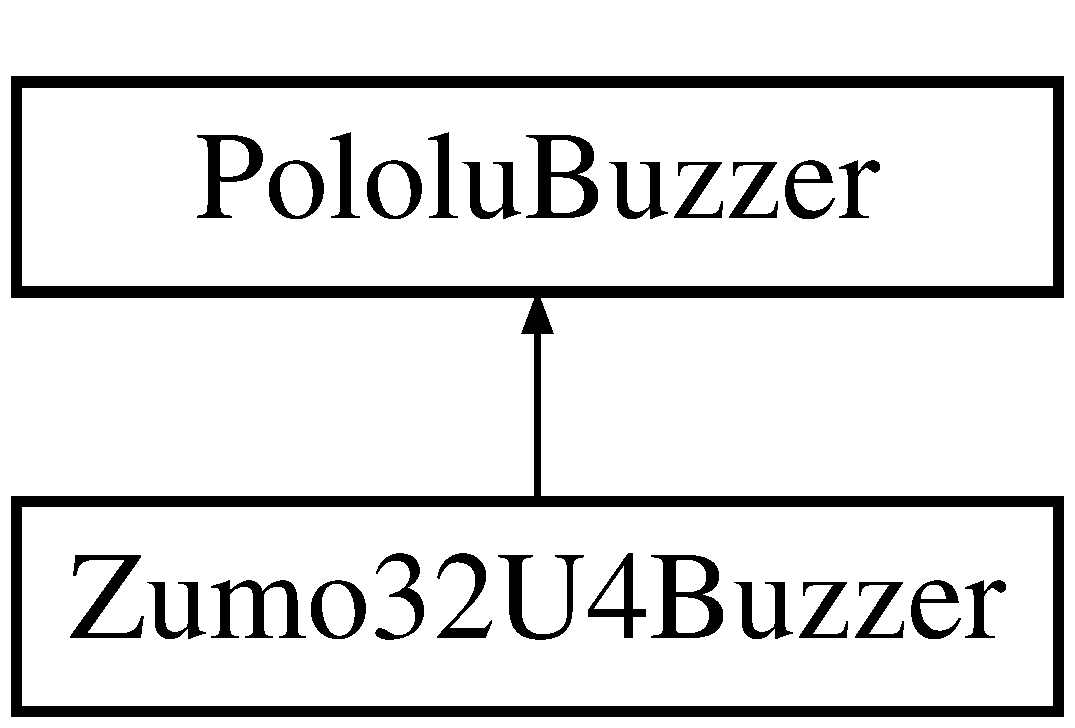
\includegraphics[height=2.000000cm]{class_zumo32_u4_buzzer}
\end{center}
\end{figure}
\doxysubsection*{Static Public Member Functions}
\begin{DoxyCompactItemize}
\item 
static void \mbox{\hyperlink{class_pololu_buzzer_a931fafd76045ae59d4ba62c9bf90b0dc}{play\+Frequency}} (unsigned int freq, unsigned int duration, unsigned char volume)
\begin{DoxyCompactList}\small\item\em Plays the specified frequency for the specified duration. \end{DoxyCompactList}\item 
static void \mbox{\hyperlink{class_pololu_buzzer_a989d410dd6cdb7abfa136c3734040fb5}{play\+Note}} (unsigned char note, unsigned int duration, unsigned char volume)
\begin{DoxyCompactList}\small\item\em Plays the specified note for the specified duration. \end{DoxyCompactList}\item 
static void \mbox{\hyperlink{class_pololu_buzzer_a22f45ef7cdf9dc8fc54e617244368277}{play}} (const char $\ast$sequence)
\begin{DoxyCompactList}\small\item\em Plays the specified sequence of notes. \end{DoxyCompactList}\item 
static void \mbox{\hyperlink{class_pololu_buzzer_a07ff4e9d9f7e4f37a58e149640b61f4e}{play\+From\+Program\+Space}} (const char $\ast$sequence)
\begin{DoxyCompactList}\small\item\em Plays the specified sequence of notes from program space. \end{DoxyCompactList}\item 
static void \mbox{\hyperlink{class_pololu_buzzer_ab72bde97ceceef8705f1bbaeccb970db}{play\+Mode}} (unsigned char mode)
\begin{DoxyCompactList}\small\item\em Controls whether {\ttfamily \mbox{\hyperlink{class_pololu_buzzer_a22f45ef7cdf9dc8fc54e617244368277}{play()}}} sequence is played automatically or must be driven with {\ttfamily \mbox{\hyperlink{class_pololu_buzzer_a427225dcc85c1e65078e4397b9890929}{play\+Check()}}}. \end{DoxyCompactList}\item 
static unsigned char \mbox{\hyperlink{class_pololu_buzzer_a427225dcc85c1e65078e4397b9890929}{play\+Check}} ()
\begin{DoxyCompactList}\small\item\em Starts the next note in a sequence, if necessary, in {\ttfamily PLAY\+\_\+\+CHECK} mode. \end{DoxyCompactList}\item 
static unsigned char \mbox{\hyperlink{class_pololu_buzzer_a8045fdf0a144e0b71a5b223a0ef34027}{is\+Playing}} ()
\begin{DoxyCompactList}\small\item\em Checks whether a note, frequency, or sequence is being played. \end{DoxyCompactList}\item 
static void \mbox{\hyperlink{class_pololu_buzzer_a233fe0ffe5f23582b1c55beaa718d527}{stop\+Playing}} ()
\begin{DoxyCompactList}\small\item\em Stops any note, frequency, or melody being played. \end{DoxyCompactList}\end{DoxyCompactItemize}


\doxysubsection{Detailed Description}
Plays beeps and music on the buzzer on the Zumo 32U4. 

This class uses Timer 4 and pin 6 (PD7/\+OC4D) to play beeps and melodies on the Zumo 32U4 buzzer.

Note durations are timed using a timer overflow interrupt ({\ttfamily TIMER4\+\_\+\+OVF}), which will briefly interrupt execution of your main program at the frequency of the sound being played. In most cases, the interrupt-\/handling routine is very short (several microseconds). However, when playing a sequence of notes in {\ttfamily PLAY\+\_\+\+AUTOMATIC} mode (the default mode) with the {\ttfamily \mbox{\hyperlink{class_pololu_buzzer_a22f45ef7cdf9dc8fc54e617244368277}{play()}}} command, this interrupt takes much longer than normal (perhaps several hundred microseconds) every time it starts a new note. It is important to take this into account when writing timing-\/critical code. 

Definition at line \mbox{\hyperlink{_zumo32_u4_buzzer_8h_source_l00023}{23}} of file \mbox{\hyperlink{_zumo32_u4_buzzer_8h_source}{Zumo32\+U4\+Buzzer.\+h}}.



\doxysubsection{Member Function Documentation}
\mbox{\Hypertarget{class_pololu_buzzer_a8045fdf0a144e0b71a5b223a0ef34027}\label{class_pololu_buzzer_a8045fdf0a144e0b71a5b223a0ef34027}} 
\index{Zumo32U4Buzzer@{Zumo32U4Buzzer}!isPlaying@{isPlaying}}
\index{isPlaying@{isPlaying}!Zumo32U4Buzzer@{Zumo32U4Buzzer}}
\doxysubsubsection{\texorpdfstring{isPlaying()}{isPlaying()}}
{\footnotesize\ttfamily unsigned char Pololu\+Buzzer\+::is\+Playing (\begin{DoxyParamCaption}{ }\end{DoxyParamCaption})\hspace{0.3cm}{\ttfamily [static]}, {\ttfamily [inherited]}}



Checks whether a note, frequency, or sequence is being played. 

\begin{DoxyReturn}{Returns}
1 if the buzzer is current playing a note, frequency, or sequence; 0 otherwise.
\end{DoxyReturn}
This method returns 1 (true) if the buzzer is currently playing a note/frequency or if it is still playing a sequence started by {\ttfamily \mbox{\hyperlink{class_pololu_buzzer_a22f45ef7cdf9dc8fc54e617244368277}{play()}}}. Otherwise, it returns 0 (false). You can poll this method to determine when it\textquotesingle{}s time to play the next note in a sequence, or you can use it as the argument to a delay loop to wait while the buzzer is busy. 

Definition at line \mbox{\hyperlink{_pololu_buzzer_8cpp_source_l00400}{400}} of file \mbox{\hyperlink{_pololu_buzzer_8cpp_source}{Pololu\+Buzzer.\+cpp}}.

\mbox{\Hypertarget{class_pololu_buzzer_a22f45ef7cdf9dc8fc54e617244368277}\label{class_pololu_buzzer_a22f45ef7cdf9dc8fc54e617244368277}} 
\index{Zumo32U4Buzzer@{Zumo32U4Buzzer}!play@{play}}
\index{play@{play}!Zumo32U4Buzzer@{Zumo32U4Buzzer}}
\doxysubsubsection{\texorpdfstring{play()}{play()}}
{\footnotesize\ttfamily void Pololu\+Buzzer\+::play (\begin{DoxyParamCaption}\item[{const char $\ast$}]{sequence }\end{DoxyParamCaption})\hspace{0.3cm}{\ttfamily [static]}, {\ttfamily [inherited]}}



Plays the specified sequence of notes. 


\begin{DoxyParams}{Parameters}
{\em sequence} & Char array containing a sequence of notes to play.\\
\hline
\end{DoxyParams}
If the play mode is {\ttfamily PLAY\+\_\+\+AUTOMATIC} (default), the sequence of notes will play with no further action required by the user. If the play mode is {\ttfamily PLAY\+\_\+\+CHECK}, the user will need to call {\ttfamily \mbox{\hyperlink{class_pololu_buzzer_a427225dcc85c1e65078e4397b9890929}{play\+Check()}}} in the main loop to initiate the playing of each new note in the sequence. The play mode can be changed while the sequence is playing. The sequence syntax is modeled after the PLAY commands in GW-\/\+BASIC, with just a few differences.

The notes are specified by the characters {\bfseries{C}}, {\bfseries{D}}, {\bfseries{E}}, {\bfseries{F}}, {\bfseries{G}}, {\bfseries{A}}, and {\bfseries{B}}, and they are played by default as \char`\"{}quarter notes\char`\"{} with a length of 500 ms. This corresponds to a tempo of 120 beats/min. Other durations can be specified by putting a number immediately after the note. For example, C8 specifies C played as an eighth note, with half the duration of a quarter note. The special note {\bfseries{R}} plays a rest (no sound). The sequence parser is case-\/insensitive and ignores spaces, which may be used to format your music nicely.

Various control characters alter the sound\+: \tabulinesep=1mm
\begin{longtabu}spread 0pt [c]{*{2}{|X[-1]}|}
\hline
\cellcolor{\tableheadbgcolor}\textbf{ Control character(s)}&\cellcolor{\tableheadbgcolor}\textbf{ Effect }\\\cline{1-2}
\endfirsthead
\hline
\endfoot
\hline
\cellcolor{\tableheadbgcolor}\textbf{ Control character(s)}&\cellcolor{\tableheadbgcolor}\textbf{ Effect }\\\cline{1-2}
\endhead
{\bfseries{A--G}} &Specifies a note that will be played. \\\cline{1-2}
{\bfseries{R}} &Specifies a rest (no sound for the duration of the note). \\\cline{1-2}
{\bfseries{+}} or {\bfseries{\#}} after a note &Raises the preceding note one half-\/step. \\\cline{1-2}
{\bfseries{-\/}} after a note &Lowers the preceding note one half-\/step. \\\cline{1-2}
{\bfseries{1--2000}} after a note &Determines the duration of the preceding note. For example, C16 specifies C played as a sixteenth note (1/16th the length of a whole note). \\\cline{1-2}
{\bfseries{.}} after a note &\char`\"{}\+Dots\char`\"{} the preceding note, increasing the length by 50\%. Each additional dot adds half as much as the previous dot, so that \char`\"{}\+A..\char`\"{} is 1.\+75 times the length of \char`\"{}\+A\char`\"{}. \\\cline{1-2}
{\bfseries{\texorpdfstring{$>$}{>}}} before a note &Plays the following note one octave higher. \\\cline{1-2}
{\bfseries{\texorpdfstring{$<$}{<}}} before a note &Plays the following note one octave lower. \\\cline{1-2}
{\bfseries{O}} followed by a number &Sets the octave. (default\+: {\bfseries{O4}}) \\\cline{1-2}
{\bfseries{T}} followed by a number &Sets the tempo in beats per minute (BPM). (default\+: {\bfseries{T120}}) \\\cline{1-2}
{\bfseries{L}} followed by a number &Sets the default note duration to the type specified by the number\+: 4 for quarter notes, 8 for eighth notes, 16 for sixteenth notes, etc. (default\+: {\bfseries{L4}}) \\\cline{1-2}
{\bfseries{V}} followed by a number &Sets the music volume (0--15). (default\+: {\bfseries{V15}}) \\\cline{1-2}
{\bfseries{MS}} &Sets all subsequent notes to play play staccato -- each note is played for 1/2 of its allotted time, followed by an equal period of silence. \\\cline{1-2}
{\bfseries{ML}} &Sets all subsequent notes to play legato -- each note is played for full length. This is the default setting. \\\cline{1-2}
{\bfseries{!}} &Resets the octave, tempo, duration, volume, and staccato setting to their default values. These settings persist from one {\ttfamily \mbox{\hyperlink{class_pololu_buzzer_a22f45ef7cdf9dc8fc54e617244368277}{play()}}} to the next, which allows you to more conveniently break up your music into reusable sections. \\\cline{1-2}
\end{longtabu}


This function plays the string of notes in the background while your program continues to execute. If you call another buzzer function while the melody is playing, the new function call will overwrite the previous and take control of the buzzer. If you want to string melodies together, you should put an appropriate delay after you start a melody playing. You can use the {\ttfamily is\+\_\+playing()} function to figure out when the buzzer is through playing the melody.\hypertarget{class_pololu_buzzer_autotoc_md1}{}\doxyparagraph{Example}\label{class_pololu_buzzer_autotoc_md1}

\begin{DoxyCode}{0}
\DoxyCodeLine{\mbox{\hyperlink{class_pololu_buzzer}{PololuBuzzer}} buzzer;}
\DoxyCodeLine{}
\DoxyCodeLine{...}
\DoxyCodeLine{}
\DoxyCodeLine{\textcolor{comment}{// play a C major scale up and back down:}}
\DoxyCodeLine{buzzer.\mbox{\hyperlink{class_pololu_buzzer_a22f45ef7cdf9dc8fc54e617244368277}{play}}(\textcolor{stringliteral}{"{}!L16 V8 cdefgab>cbagfedc"{}});}
\DoxyCodeLine{\textcolor{keywordflow}{while} (buzzer.\mbox{\hyperlink{class_pololu_buzzer_a8045fdf0a144e0b71a5b223a0ef34027}{isPlaying}}());}
\DoxyCodeLine{}
\DoxyCodeLine{\textcolor{comment}{// the first few measures of Bach's fugue in D-\/minor}}
\DoxyCodeLine{buzzer.\mbox{\hyperlink{class_pololu_buzzer_a22f45ef7cdf9dc8fc54e617244368277}{play}}(\textcolor{stringliteral}{"{}!T240 L8 agafaea dac+adaea fa<aa<bac\#a dac\#adaea f4"{}});}

\end{DoxyCode}
 

Definition at line \mbox{\hyperlink{_pololu_buzzer_8cpp_source_l00463}{463}} of file \mbox{\hyperlink{_pololu_buzzer_8cpp_source}{Pololu\+Buzzer.\+cpp}}.

\mbox{\Hypertarget{class_pololu_buzzer_a427225dcc85c1e65078e4397b9890929}\label{class_pololu_buzzer_a427225dcc85c1e65078e4397b9890929}} 
\index{Zumo32U4Buzzer@{Zumo32U4Buzzer}!playCheck@{playCheck}}
\index{playCheck@{playCheck}!Zumo32U4Buzzer@{Zumo32U4Buzzer}}
\doxysubsubsection{\texorpdfstring{playCheck()}{playCheck()}}
{\footnotesize\ttfamily unsigned char Pololu\+Buzzer\+::play\+Check (\begin{DoxyParamCaption}{ }\end{DoxyParamCaption})\hspace{0.3cm}{\ttfamily [static]}, {\ttfamily [inherited]}}



Starts the next note in a sequence, if necessary, in {\ttfamily PLAY\+\_\+\+CHECK} mode. 

\begin{DoxyReturn}{Returns}
0 if sequence is complete, 1 otherwise.
\end{DoxyReturn}
This method only needs to be called if you are in {\ttfamily PLAY\+\_\+\+CHECK} mode. It checks to see whether it is time to start another note in the sequence initiated by {\ttfamily \mbox{\hyperlink{class_pololu_buzzer_a22f45ef7cdf9dc8fc54e617244368277}{play()}}}, and starts it if so. If it is not yet time to start the next note, this method returns without doing anything. Call this as often as possible in your main loop to avoid delays between notes in the sequence. This method returns 0 (false) if the melody to be played is complete, otherwise it returns 1 (true). 

Definition at line \mbox{\hyperlink{_pololu_buzzer_8cpp_source_l00725}{725}} of file \mbox{\hyperlink{_pololu_buzzer_8cpp_source}{Pololu\+Buzzer.\+cpp}}.

\mbox{\Hypertarget{class_pololu_buzzer_a931fafd76045ae59d4ba62c9bf90b0dc}\label{class_pololu_buzzer_a931fafd76045ae59d4ba62c9bf90b0dc}} 
\index{Zumo32U4Buzzer@{Zumo32U4Buzzer}!playFrequency@{playFrequency}}
\index{playFrequency@{playFrequency}!Zumo32U4Buzzer@{Zumo32U4Buzzer}}
\doxysubsubsection{\texorpdfstring{playFrequency()}{playFrequency()}}
{\footnotesize\ttfamily void Pololu\+Buzzer\+::play\+Frequency (\begin{DoxyParamCaption}\item[{unsigned int}]{freq,  }\item[{unsigned int}]{duration,  }\item[{unsigned char}]{volume }\end{DoxyParamCaption})\hspace{0.3cm}{\ttfamily [static]}, {\ttfamily [inherited]}}



Plays the specified frequency for the specified duration. 


\begin{DoxyParams}{Parameters}
{\em freq} & Frequency to play in Hz (or 0.\+1 Hz if the {\ttfamily DIV\+\_\+\+BY\+\_\+10} bit is set). \\
\hline
{\em duration} & Duration of the note in milliseconds. \\
\hline
{\em volume} & Volume of the note (0--15).\\
\hline
\end{DoxyParams}
The {\itshape frequency} argument must be between 40 Hz and 10 k\+Hz. If the most significant bit of {\itshape frequency} is set, the frequency played is the value of the lower 15 bits of {\itshape frequency} in units of 0.\+1 Hz. Therefore, you can play a frequency of 44.\+5 Hz by using a {\itshape frequency} of {\ttfamily (DIV\+\_\+\+BY\+\_\+10 $\vert$ 445)}. If the most significant bit of {\itshape frequency} is not set, the units for frequency are Hz. The {\itshape volume} argument controls the buzzer volume, with 15 being the loudest and 0 being the quietest. A {\itshape volume} of 15 supplies the buzzer with a 50\% duty cycle PWM at the specified {\itshape frequency}. Lowering {\itshape volume} by one halves the duty cycle (so 14 gives a 25\% duty cycle, 13 gives a 12.\+5\% duty cycle, etc). The volume control is somewhat crude (especially on the ATmega328/168) and should be thought of as a bonus feature.

This function plays the note in the background while your program continues to execute. If you call another buzzer function while the note is playing, the new function call will overwrite the previous and take control of the buzzer. If you want to string notes together, you should either use the {\ttfamily \mbox{\hyperlink{class_pololu_buzzer_a22f45ef7cdf9dc8fc54e617244368277}{play()}}} function or put an appropriate delay after you start a note playing. You can use the {\ttfamily is\+\_\+playing()} function to figure out when the buzzer is through playing its note or melody.\hypertarget{class_pololu_buzzer_autotoc_md0}{}\doxyparagraph{Example}\label{class_pololu_buzzer_autotoc_md0}

\begin{DoxyCode}{0}
\DoxyCodeLine{\mbox{\hyperlink{class_pololu_buzzer}{PololuBuzzer}} buzzer;}
\DoxyCodeLine{}
\DoxyCodeLine{...}
\DoxyCodeLine{}
\DoxyCodeLine{\textcolor{comment}{// play a 6 kHz note for 250 ms at a lower volume}}
\DoxyCodeLine{buzzer.\mbox{\hyperlink{class_pololu_buzzer_a931fafd76045ae59d4ba62c9bf90b0dc}{playFrequency}}(6000, 250, 12);}
\DoxyCodeLine{}
\DoxyCodeLine{\textcolor{comment}{// wait for buzzer to finish playing the note}}
\DoxyCodeLine{\textcolor{keywordflow}{while} (buzzer.\mbox{\hyperlink{class_pololu_buzzer_a8045fdf0a144e0b71a5b223a0ef34027}{isPlaying}}());}
\DoxyCodeLine{}
\DoxyCodeLine{\textcolor{comment}{// play a 44.5 Hz note for 1 s at full volume}}
\DoxyCodeLine{buzzer.\mbox{\hyperlink{class_pololu_buzzer_a931fafd76045ae59d4ba62c9bf90b0dc}{playFrequency}}(\mbox{\hyperlink{_pololu_buzzer_8h_a8548d3f2b6d5fa2bcc350fad4a2c72a8}{DIV\_BY\_10}} | 445, 1000, 15);}

\end{DoxyCode}


\begin{DoxyWarning}{Warning}
{\itshape frequency} {$\times$} {\itshape duration} / 1000 must be no greater than 0x\+FFFF (65535). This means you can\textquotesingle{}t use a duration of 65535 ms for frequencies greater than 1 k\+Hz. For example, the maximum duration you can use for a frequency of 10 k\+Hz is 6553 ms. If you use a duration longer than this, you will produce an integer overflow that can result in unexpected behavior. 
\end{DoxyWarning}


Definition at line \mbox{\hyperlink{_pololu_buzzer_8cpp_source_l00199}{199}} of file \mbox{\hyperlink{_pololu_buzzer_8cpp_source}{Pololu\+Buzzer.\+cpp}}.

\mbox{\Hypertarget{class_pololu_buzzer_a07ff4e9d9f7e4f37a58e149640b61f4e}\label{class_pololu_buzzer_a07ff4e9d9f7e4f37a58e149640b61f4e}} 
\index{Zumo32U4Buzzer@{Zumo32U4Buzzer}!playFromProgramSpace@{playFromProgramSpace}}
\index{playFromProgramSpace@{playFromProgramSpace}!Zumo32U4Buzzer@{Zumo32U4Buzzer}}
\doxysubsubsection{\texorpdfstring{playFromProgramSpace()}{playFromProgramSpace()}}
{\footnotesize\ttfamily void Pololu\+Buzzer\+::play\+From\+Program\+Space (\begin{DoxyParamCaption}\item[{const char $\ast$}]{sequence }\end{DoxyParamCaption})\hspace{0.3cm}{\ttfamily [static]}, {\ttfamily [inherited]}}



Plays the specified sequence of notes from program space. 


\begin{DoxyParams}{Parameters}
{\em sequence} & Char array in program space containing a sequence of notes to play.\\
\hline
\end{DoxyParams}
A version of {\ttfamily \mbox{\hyperlink{class_pololu_buzzer_a22f45ef7cdf9dc8fc54e617244368277}{play()}}} that takes a pointer to program space instead of RAM. This is desirable since RAM is limited and the string must be in program space anyway.\hypertarget{class_pololu_buzzer_autotoc_md2}{}\doxyparagraph{Example}\label{class_pololu_buzzer_autotoc_md2}

\begin{DoxyCode}{0}
\DoxyCodeLine{\textcolor{preprocessor}{\#include <avr/pgmspace.h>}}
\DoxyCodeLine{}
\DoxyCodeLine{\mbox{\hyperlink{class_pololu_buzzer}{PololuBuzzer}} buzzer;}
\DoxyCodeLine{\textcolor{keyword}{const} \textcolor{keywordtype}{char} melody[] PROGMEM = \textcolor{stringliteral}{"{}!L16 V8 cdefgab>cbagfedc"{}};}
\DoxyCodeLine{}
\DoxyCodeLine{...}
\DoxyCodeLine{}
\DoxyCodeLine{buzzer.\mbox{\hyperlink{class_pololu_buzzer_a07ff4e9d9f7e4f37a58e149640b61f4e}{playFromProgramSpace}}(melody);}

\end{DoxyCode}
 

Definition at line \mbox{\hyperlink{_pololu_buzzer_8cpp_source_l00472}{472}} of file \mbox{\hyperlink{_pololu_buzzer_8cpp_source}{Pololu\+Buzzer.\+cpp}}.

\mbox{\Hypertarget{class_pololu_buzzer_ab72bde97ceceef8705f1bbaeccb970db}\label{class_pololu_buzzer_ab72bde97ceceef8705f1bbaeccb970db}} 
\index{Zumo32U4Buzzer@{Zumo32U4Buzzer}!playMode@{playMode}}
\index{playMode@{playMode}!Zumo32U4Buzzer@{Zumo32U4Buzzer}}
\doxysubsubsection{\texorpdfstring{playMode()}{playMode()}}
{\footnotesize\ttfamily void Pololu\+Buzzer\+::play\+Mode (\begin{DoxyParamCaption}\item[{unsigned char}]{mode }\end{DoxyParamCaption})\hspace{0.3cm}{\ttfamily [static]}, {\ttfamily [inherited]}}



Controls whether {\ttfamily \mbox{\hyperlink{class_pololu_buzzer_a22f45ef7cdf9dc8fc54e617244368277}{play()}}} sequence is played automatically or must be driven with {\ttfamily \mbox{\hyperlink{class_pololu_buzzer_a427225dcc85c1e65078e4397b9890929}{play\+Check()}}}. 


\begin{DoxyParams}{Parameters}
{\em mode} & Play mode (either {\ttfamily PLAY\+\_\+\+AUTOMATIC} or {\ttfamily PLAY\+\_\+\+CHECK}).\\
\hline
\end{DoxyParams}
This method lets you determine whether the notes of the {\ttfamily \mbox{\hyperlink{class_pololu_buzzer_a22f45ef7cdf9dc8fc54e617244368277}{play()}}} sequence are played automatically in the background or are driven by the {\ttfamily \mbox{\hyperlink{class_pololu_buzzer_a427225dcc85c1e65078e4397b9890929}{play\+Check()}}} method. If {\itshape mode} is {\ttfamily PLAY\+\_\+\+AUTOMATIC}, the sequence will play automatically in the background, driven by the timer overflow interrupt. The interrupt will take a considerable amount of time to execute when it starts the next note in the sequence playing, so it is recommended that you do not use automatic-\/play if you cannot tolerate being interrupted for more than a few microseconds. If {\itshape mode} is {\ttfamily PLAY\+\_\+\+CHECK}, you can control when the next note in the sequence is played by calling the {\ttfamily \mbox{\hyperlink{class_pololu_buzzer_a427225dcc85c1e65078e4397b9890929}{play\+Check()}}} method at acceptable points in your main loop. If your main loop has substantial delays, it is recommended that you use automatic-\/play mode rather than play-\/check mode. Note that the play mode can be changed while the sequence is being played. The mode is set to {\ttfamily PLAY\+\_\+\+AUTOMATIC} by default. 

Definition at line \mbox{\hyperlink{_pololu_buzzer_8cpp_source_l00708}{708}} of file \mbox{\hyperlink{_pololu_buzzer_8cpp_source}{Pololu\+Buzzer.\+cpp}}.

\mbox{\Hypertarget{class_pololu_buzzer_a989d410dd6cdb7abfa136c3734040fb5}\label{class_pololu_buzzer_a989d410dd6cdb7abfa136c3734040fb5}} 
\index{Zumo32U4Buzzer@{Zumo32U4Buzzer}!playNote@{playNote}}
\index{playNote@{playNote}!Zumo32U4Buzzer@{Zumo32U4Buzzer}}
\doxysubsubsection{\texorpdfstring{playNote()}{playNote()}}
{\footnotesize\ttfamily void Pololu\+Buzzer\+::play\+Note (\begin{DoxyParamCaption}\item[{unsigned char}]{note,  }\item[{unsigned int}]{duration,  }\item[{unsigned char}]{volume }\end{DoxyParamCaption})\hspace{0.3cm}{\ttfamily [static]}, {\ttfamily [inherited]}}



Plays the specified note for the specified duration. 


\begin{DoxyParams}{Parameters}
{\em note} & Note to play (see \mbox{\hyperlink{_pololu_buzzer_8h_note_macros}{Note Macros}}). \\
\hline
{\em duration} & Duration of the note in milliseconds. \\
\hline
{\em volume} & Volume of the note (0--15).\\
\hline
\end{DoxyParams}
The {\itshape note} argument is an enumeration for the notes of the equal tempered scale (ETS). See \mbox{\hyperlink{_pololu_buzzer_8h_note_macros}{Note Macros}} for more information. The {\itshape volume} argument controls the buzzer volume, with 15 being the loudest and 0 being the quietest. A {\itshape volume} of 15 supplies the buzzer with a 50\% duty cycle PWM at the specified {\itshape frequency}. Lowering {\itshape volume} by one halves the duty cycle (so 14 gives a 25\% duty cycle, 13 gives a 12.\+5\% duty cycle, etc). The volume control is somewhat crude (especially on the ATmega328/168) and should be thought of as a bonus feature.

This function plays the note in the background while your program continues to execute. If you call another buzzer function while the note is playing, the new function call will overwrite the previous and take control of the buzzer. If you want to string notes together, you should either use the {\ttfamily \mbox{\hyperlink{class_pololu_buzzer_a22f45ef7cdf9dc8fc54e617244368277}{play()}}} function or put an appropriate delay after you start a note playing. You can use the {\ttfamily is\+\_\+playing()} function to figure out when the buzzer is through playing its note or melody. 

Definition at line \mbox{\hyperlink{_pololu_buzzer_8cpp_source_l00294}{294}} of file \mbox{\hyperlink{_pololu_buzzer_8cpp_source}{Pololu\+Buzzer.\+cpp}}.

\mbox{\Hypertarget{class_pololu_buzzer_a233fe0ffe5f23582b1c55beaa718d527}\label{class_pololu_buzzer_a233fe0ffe5f23582b1c55beaa718d527}} 
\index{Zumo32U4Buzzer@{Zumo32U4Buzzer}!stopPlaying@{stopPlaying}}
\index{stopPlaying@{stopPlaying}!Zumo32U4Buzzer@{Zumo32U4Buzzer}}
\doxysubsubsection{\texorpdfstring{stopPlaying()}{stopPlaying()}}
{\footnotesize\ttfamily void Pololu\+Buzzer\+::stop\+Playing (\begin{DoxyParamCaption}{ }\end{DoxyParamCaption})\hspace{0.3cm}{\ttfamily [static]}, {\ttfamily [inherited]}}



Stops any note, frequency, or melody being played. 

This method will immediately silence the buzzer and terminate any note/frequency/melody that is currently playing. 

Definition at line \mbox{\hyperlink{_pololu_buzzer_8cpp_source_l00483}{483}} of file \mbox{\hyperlink{_pololu_buzzer_8cpp_source}{Pololu\+Buzzer.\+cpp}}.



The documentation for this class was generated from the following file\+:\begin{DoxyCompactItemize}
\item 
\mbox{\hyperlink{_zumo32_u4_buzzer_8h}{Zumo32\+U4\+Buzzer.\+h}}\end{DoxyCompactItemize}

\hypertarget{class_zumo32_u4_encoders}{}\doxysection{Zumo32\+U4\+Encoders Class Reference}
\label{class_zumo32_u4_encoders}\index{Zumo32U4Encoders@{Zumo32U4Encoders}}


Reads counts from the encoders on the Zumo 32U4.  




{\ttfamily \#include $<$Zumo32\+U4\+Encoders.\+h$>$}

\doxysubsection*{Static Public Member Functions}
\begin{DoxyCompactItemize}
\item 
static void \mbox{\hyperlink{class_zumo32_u4_encoders_afa1199db1c88dce2e42a461dc45df560}{init}} ()
\item 
static int16\+\_\+t \mbox{\hyperlink{class_zumo32_u4_encoders_a142d33610a12b209e257c1635b2daae6}{get\+Counts\+Left}} ()
\item 
static int16\+\_\+t \mbox{\hyperlink{class_zumo32_u4_encoders_ad570df0c84cbb719dc975233b4f65756}{get\+Counts\+Right}} ()
\item 
static int16\+\_\+t \mbox{\hyperlink{class_zumo32_u4_encoders_a9b212103e652d1edb9d622381c303497}{get\+Counts\+And\+Reset\+Left}} ()
\item 
static int16\+\_\+t \mbox{\hyperlink{class_zumo32_u4_encoders_a613358c24dbc997cb9fee36d66bbf2ba}{get\+Counts\+And\+Reset\+Right}} ()
\item 
static bool \mbox{\hyperlink{class_zumo32_u4_encoders_ad20765947ef87f562a4a19975a7fb9ca}{check\+Error\+Left}} ()
\item 
static bool \mbox{\hyperlink{class_zumo32_u4_encoders_a9d7de11def7409becbe870056ef2d719}{check\+Error\+Right}} ()
\end{DoxyCompactItemize}


\doxysubsection{Detailed Description}
Reads counts from the encoders on the Zumo 32U4. 

This class allows you to read counts from the encoders on the Zumo 32U4, which lets you tell how much each motor has turned and in what direction.

The encoders are monitored in the background using interrupts, so your code can perform other tasks without missing encoder counts.

To read the left encoder, this class uses an interrupt service routine (ISR) for PCINT0\+\_\+vect, so there will be a compile-\/time conflict with any other code that defines a pin-\/change ISR.

To read the right encoder, this class calls \href{http://arduino.cc/en/Reference/attachInterrupt}{\texttt{ attach\+Interrupt()}}, so there will be a compile-\/time conflict with any other code that defines an ISR for an external interrupt directly instead of using attach\+Interrupt(). 

Definition at line 25 of file Zumo32\+U4\+Encoders.\+h.



\doxysubsection{Member Function Documentation}
\mbox{\Hypertarget{class_zumo32_u4_encoders_ad20765947ef87f562a4a19975a7fb9ca}\label{class_zumo32_u4_encoders_ad20765947ef87f562a4a19975a7fb9ca}} 
\index{Zumo32U4Encoders@{Zumo32U4Encoders}!checkErrorLeft@{checkErrorLeft}}
\index{checkErrorLeft@{checkErrorLeft}!Zumo32U4Encoders@{Zumo32U4Encoders}}
\doxysubsubsection{\texorpdfstring{checkErrorLeft()}{checkErrorLeft()}}
{\footnotesize\ttfamily bool Zumo32\+U4\+Encoders\+::check\+Error\+Left (\begin{DoxyParamCaption}{ }\end{DoxyParamCaption})\hspace{0.3cm}{\ttfamily [static]}}

This function returns true if an error was detected on the left-\/side encoder. It resets the error flag automatically, so it will only return true if an error was detected since the last time \mbox{\hyperlink{class_zumo32_u4_encoders_ad20765947ef87f562a4a19975a7fb9ca}{check\+Error\+Left()}} was called.

If an error happens, it means that both of the encoder outputs changed at the same time from the perspective of the ISR, so the ISR was unable to tell what direction the motor was moving, and the encoder count could be inaccurate. The most likely cause for an error is that the interrupt service routine for the encoders could not be started soon enough. If you get encoder errors, make sure you are not disabling interrupts for extended periods of time in your code. 

Definition at line 133 of file Zumo32\+U4\+Encoders.\+cpp.

\mbox{\Hypertarget{class_zumo32_u4_encoders_a9d7de11def7409becbe870056ef2d719}\label{class_zumo32_u4_encoders_a9d7de11def7409becbe870056ef2d719}} 
\index{Zumo32U4Encoders@{Zumo32U4Encoders}!checkErrorRight@{checkErrorRight}}
\index{checkErrorRight@{checkErrorRight}!Zumo32U4Encoders@{Zumo32U4Encoders}}
\doxysubsubsection{\texorpdfstring{checkErrorRight()}{checkErrorRight()}}
{\footnotesize\ttfamily bool Zumo32\+U4\+Encoders\+::check\+Error\+Right (\begin{DoxyParamCaption}{ }\end{DoxyParamCaption})\hspace{0.3cm}{\ttfamily [static]}}

This function is just like \mbox{\hyperlink{class_zumo32_u4_encoders_ad20765947ef87f562a4a19975a7fb9ca}{check\+Error\+Left()}} except it applies to the right-\/side encoder. 

Definition at line 142 of file Zumo32\+U4\+Encoders.\+cpp.

\mbox{\Hypertarget{class_zumo32_u4_encoders_a9b212103e652d1edb9d622381c303497}\label{class_zumo32_u4_encoders_a9b212103e652d1edb9d622381c303497}} 
\index{Zumo32U4Encoders@{Zumo32U4Encoders}!getCountsAndResetLeft@{getCountsAndResetLeft}}
\index{getCountsAndResetLeft@{getCountsAndResetLeft}!Zumo32U4Encoders@{Zumo32U4Encoders}}
\doxysubsubsection{\texorpdfstring{getCountsAndResetLeft()}{getCountsAndResetLeft()}}
{\footnotesize\ttfamily int16\+\_\+t Zumo32\+U4\+Encoders\+::get\+Counts\+And\+Reset\+Left (\begin{DoxyParamCaption}{ }\end{DoxyParamCaption})\hspace{0.3cm}{\ttfamily [static]}}

This function is just like \mbox{\hyperlink{class_zumo32_u4_encoders_a142d33610a12b209e257c1635b2daae6}{get\+Counts\+Left()}} except it also clears the counts before returning. If you call this frequently enough, you will not have to worry about the count overflowing. 

Definition at line 111 of file Zumo32\+U4\+Encoders.\+cpp.

\mbox{\Hypertarget{class_zumo32_u4_encoders_a613358c24dbc997cb9fee36d66bbf2ba}\label{class_zumo32_u4_encoders_a613358c24dbc997cb9fee36d66bbf2ba}} 
\index{Zumo32U4Encoders@{Zumo32U4Encoders}!getCountsAndResetRight@{getCountsAndResetRight}}
\index{getCountsAndResetRight@{getCountsAndResetRight}!Zumo32U4Encoders@{Zumo32U4Encoders}}
\doxysubsubsection{\texorpdfstring{getCountsAndResetRight()}{getCountsAndResetRight()}}
{\footnotesize\ttfamily int16\+\_\+t Zumo32\+U4\+Encoders\+::get\+Counts\+And\+Reset\+Right (\begin{DoxyParamCaption}{ }\end{DoxyParamCaption})\hspace{0.3cm}{\ttfamily [static]}}

This function is just like \mbox{\hyperlink{class_zumo32_u4_encoders_a9b212103e652d1edb9d622381c303497}{get\+Counts\+And\+Reset\+Left()}} except it applies to the right-\/side encoder. 

Definition at line 122 of file Zumo32\+U4\+Encoders.\+cpp.

\mbox{\Hypertarget{class_zumo32_u4_encoders_a142d33610a12b209e257c1635b2daae6}\label{class_zumo32_u4_encoders_a142d33610a12b209e257c1635b2daae6}} 
\index{Zumo32U4Encoders@{Zumo32U4Encoders}!getCountsLeft@{getCountsLeft}}
\index{getCountsLeft@{getCountsLeft}!Zumo32U4Encoders@{Zumo32U4Encoders}}
\doxysubsubsection{\texorpdfstring{getCountsLeft()}{getCountsLeft()}}
{\footnotesize\ttfamily int16\+\_\+t Zumo32\+U4\+Encoders\+::get\+Counts\+Left (\begin{DoxyParamCaption}{ }\end{DoxyParamCaption})\hspace{0.3cm}{\ttfamily [static]}}

Returns the number of counts that have been detected from the left-\/side encoder. These counts start at 0. Positive counts correspond to forward movement of the left side of the Zumo, while negative counts correspond to backwards movement.

The count is returned as a signed 16-\/bit integer. When the count goes over 32767, it will overflow down to -\/32768. When the count goes below -\/32768, it will overflow up to 32767. 

Definition at line 91 of file Zumo32\+U4\+Encoders.\+cpp.

\mbox{\Hypertarget{class_zumo32_u4_encoders_ad570df0c84cbb719dc975233b4f65756}\label{class_zumo32_u4_encoders_ad570df0c84cbb719dc975233b4f65756}} 
\index{Zumo32U4Encoders@{Zumo32U4Encoders}!getCountsRight@{getCountsRight}}
\index{getCountsRight@{getCountsRight}!Zumo32U4Encoders@{Zumo32U4Encoders}}
\doxysubsubsection{\texorpdfstring{getCountsRight()}{getCountsRight()}}
{\footnotesize\ttfamily int16\+\_\+t Zumo32\+U4\+Encoders\+::get\+Counts\+Right (\begin{DoxyParamCaption}{ }\end{DoxyParamCaption})\hspace{0.3cm}{\ttfamily [static]}}

This function is just like \mbox{\hyperlink{class_zumo32_u4_encoders_a142d33610a12b209e257c1635b2daae6}{get\+Counts\+Left()}} except it applies to the right-\/side encoder. 

Definition at line 101 of file Zumo32\+U4\+Encoders.\+cpp.

\mbox{\Hypertarget{class_zumo32_u4_encoders_afa1199db1c88dce2e42a461dc45df560}\label{class_zumo32_u4_encoders_afa1199db1c88dce2e42a461dc45df560}} 
\index{Zumo32U4Encoders@{Zumo32U4Encoders}!init@{init}}
\index{init@{init}!Zumo32U4Encoders@{Zumo32U4Encoders}}
\doxysubsubsection{\texorpdfstring{init()}{init()}}
{\footnotesize\ttfamily static void Zumo32\+U4\+Encoders\+::init (\begin{DoxyParamCaption}{ }\end{DoxyParamCaption})\hspace{0.3cm}{\ttfamily [inline]}, {\ttfamily [static]}}

This function initializes the encoders if they have not been initialized already and starts listening for counts. This function is called automatically whenever you call any other function in this class, so you should not normally need to call it in your code. 

Definition at line 34 of file Zumo32\+U4\+Encoders.\+h.



The documentation for this class was generated from the following files\+:\begin{DoxyCompactItemize}
\item 
\mbox{\hyperlink{_zumo32_u4_encoders_8h}{Zumo32\+U4\+Encoders.\+h}}\item 
Zumo32\+U4\+Encoders.\+cpp\end{DoxyCompactItemize}

\hypertarget{class_zumo32_u4_i_m_u}{}\section{Zumo32\+U4\+I\+MU Class Reference}
\label{class_zumo32_u4_i_m_u}\index{Zumo32\+U4\+I\+MU@{Zumo32\+U4\+I\+MU}}


Interfaces with the inertial sensors on the Zumo 32\+U4.  




{\ttfamily \#include $<$Zumo32\+U4\+I\+M\+U.\+h$>$}

\subsection*{Classes}
\begin{DoxyCompactItemize}
\item 
struct \hyperlink{struct_zumo32_u4_i_m_u_1_1vector}{vector}
\begin{DoxyCompactList}\small\item\em Represents a 3-\/dimensional vector with x, y, and z components. \end{DoxyCompactList}\end{DoxyCompactItemize}
\subsection*{Public Member Functions}
\begin{DoxyCompactItemize}
\item 
\mbox{\Hypertarget{class_zumo32_u4_i_m_u_ad00f3ac13787ecb7cc0c3b7d4428fd5b}\label{class_zumo32_u4_i_m_u_ad00f3ac13787ecb7cc0c3b7d4428fd5b}} 
uint8\+\_\+t \hyperlink{class_zumo32_u4_i_m_u_ad00f3ac13787ecb7cc0c3b7d4428fd5b}{get\+Last\+Error} ()
\begin{DoxyCompactList}\small\item\em Returns 0 if the last I2C communication with the I\+MU was successful, or a non-\/zero status code if there was an error. \end{DoxyCompactList}\item 
bool \hyperlink{class_zumo32_u4_i_m_u_aca2ae4fe4989453c2e4f73e9dc7439d2}{init} ()
\begin{DoxyCompactList}\small\item\em Initializes the inertial sensors and detects their type. \end{DoxyCompactList}\item 
\hyperlink{_zumo32_u4_i_m_u_8h_a2be3e50a86f638af5bb120cc740f3452}{Zumo32\+U4\+I\+M\+U\+Type} \hyperlink{class_zumo32_u4_i_m_u_a936427abfbed839c5669746d274427bd}{get\+Type} ()
\begin{DoxyCompactList}\small\item\em Returns the type of the inertial sensors on the Zumo 32\+U4. \end{DoxyCompactList}\item 
\mbox{\Hypertarget{class_zumo32_u4_i_m_u_acfb1ce51ff908de9635ccbc3652a3fbb}\label{class_zumo32_u4_i_m_u_acfb1ce51ff908de9635ccbc3652a3fbb}} 
void \hyperlink{class_zumo32_u4_i_m_u_acfb1ce51ff908de9635ccbc3652a3fbb}{enable\+Default} ()
\begin{DoxyCompactList}\small\item\em Enables all of the inertial sensors with a default configuration. \end{DoxyCompactList}\item 
\mbox{\Hypertarget{class_zumo32_u4_i_m_u_ad166edc8fb6304c2f5329ebc490f21ad}\label{class_zumo32_u4_i_m_u_ad166edc8fb6304c2f5329ebc490f21ad}} 
void \hyperlink{class_zumo32_u4_i_m_u_ad166edc8fb6304c2f5329ebc490f21ad}{configure\+For\+Turn\+Sensing} ()
\begin{DoxyCompactList}\small\item\em Configures the sensors with settings optimized for turn sensing. \end{DoxyCompactList}\item 
\mbox{\Hypertarget{class_zumo32_u4_i_m_u_a78786abfc220e14ebb603b72dce8f4ca}\label{class_zumo32_u4_i_m_u_a78786abfc220e14ebb603b72dce8f4ca}} 
void \hyperlink{class_zumo32_u4_i_m_u_a78786abfc220e14ebb603b72dce8f4ca}{configure\+For\+Balancing} ()
\begin{DoxyCompactList}\small\item\em Configures the sensors with settings optimized for balancing. \end{DoxyCompactList}\item 
\mbox{\Hypertarget{class_zumo32_u4_i_m_u_af9992e0ff9c372edc8d3a5d165411263}\label{class_zumo32_u4_i_m_u_af9992e0ff9c372edc8d3a5d165411263}} 
void \hyperlink{class_zumo32_u4_i_m_u_af9992e0ff9c372edc8d3a5d165411263}{configure\+For\+Face\+Uphill} ()
\begin{DoxyCompactList}\small\item\em Configures the sensors with settings optimized for the Face\+Uphill example program. \end{DoxyCompactList}\item 
void \hyperlink{class_zumo32_u4_i_m_u_ab5cb0c1c2342386c13afe36f7064d1e8}{write\+Reg} (uint8\+\_\+t addr, uint8\+\_\+t reg, uint8\+\_\+t value)
\begin{DoxyCompactList}\small\item\em Writes an 8-\/bit sensor register. \end{DoxyCompactList}\item 
uint8\+\_\+t \hyperlink{class_zumo32_u4_i_m_u_a8bc90dccbd0259a97a5f0bd1e8f0316a}{read\+Reg} (uint8\+\_\+t addr, uint8\+\_\+t reg)
\begin{DoxyCompactList}\small\item\em Reads an 8-\/bit sensor register. \end{DoxyCompactList}\item 
\mbox{\Hypertarget{class_zumo32_u4_i_m_u_a034c243ac0be1892af67c71759aa577c}\label{class_zumo32_u4_i_m_u_a034c243ac0be1892af67c71759aa577c}} 
void \hyperlink{class_zumo32_u4_i_m_u_a034c243ac0be1892af67c71759aa577c}{read\+Acc} ()
\begin{DoxyCompactList}\small\item\em Takes a reading from the accelerometer and makes the measurements available in \hyperlink{class_zumo32_u4_i_m_u_a386b34407b744844d403e5e0041dc475}{a}. \end{DoxyCompactList}\item 
\mbox{\Hypertarget{class_zumo32_u4_i_m_u_a1c460bf87ffc7d671b398bf9ef4951d6}\label{class_zumo32_u4_i_m_u_a1c460bf87ffc7d671b398bf9ef4951d6}} 
void \hyperlink{class_zumo32_u4_i_m_u_a1c460bf87ffc7d671b398bf9ef4951d6}{read\+Gyro} ()
\begin{DoxyCompactList}\small\item\em Takes a reading from the gyro and makes the measurements available in \hyperlink{class_zumo32_u4_i_m_u_a6870acdcde72d4f3ec2bd70088641e4e}{g}. \end{DoxyCompactList}\item 
\mbox{\Hypertarget{class_zumo32_u4_i_m_u_a83f3ef3030e781ea7cee727190f3bd2d}\label{class_zumo32_u4_i_m_u_a83f3ef3030e781ea7cee727190f3bd2d}} 
void \hyperlink{class_zumo32_u4_i_m_u_a83f3ef3030e781ea7cee727190f3bd2d}{read\+Mag} ()
\begin{DoxyCompactList}\small\item\em Takes a reading from the magnetometer and makes the measurements available in \hyperlink{class_zumo32_u4_i_m_u_a667705e0bbee3b4b5ec3a49b2fc72662}{m}. \end{DoxyCompactList}\item 
\mbox{\Hypertarget{class_zumo32_u4_i_m_u_aad16780f526df9f77614f47427c658ed}\label{class_zumo32_u4_i_m_u_aad16780f526df9f77614f47427c658ed}} 
void \hyperlink{class_zumo32_u4_i_m_u_aad16780f526df9f77614f47427c658ed}{read} ()
\begin{DoxyCompactList}\small\item\em Takes a reading from all three sensors (accelerometer, gyro, and magnetometer) and makes their measurements available in the respective vectors. \end{DoxyCompactList}\item 
bool \hyperlink{class_zumo32_u4_i_m_u_a75735024206bd09d0905f28455f0a368}{acc\+Data\+Ready} ()
\begin{DoxyCompactList}\small\item\em Indicates whether the accelerometer has new measurement data ready. \end{DoxyCompactList}\item 
bool \hyperlink{class_zumo32_u4_i_m_u_a82a4b99d45afb0b5008e32213fa2e0cc}{gyro\+Data\+Ready} ()
\begin{DoxyCompactList}\small\item\em Indicates whether the gyro has new measurement data ready. \end{DoxyCompactList}\item 
bool \hyperlink{class_zumo32_u4_i_m_u_ad9a7bde2fa435b4ceb6929e73acef4b6}{mag\+Data\+Ready} ()
\begin{DoxyCompactList}\small\item\em Indicates whether the magnetometer has new measurement data ready. \end{DoxyCompactList}\end{DoxyCompactItemize}
\subsection*{Public Attributes}
\begin{DoxyCompactItemize}
\item 
\mbox{\Hypertarget{class_zumo32_u4_i_m_u_a386b34407b744844d403e5e0041dc475}\label{class_zumo32_u4_i_m_u_a386b34407b744844d403e5e0041dc475}} 
\hyperlink{struct_zumo32_u4_i_m_u_1_1vector}{vector}$<$ int16\+\_\+t $>$ \hyperlink{class_zumo32_u4_i_m_u_a386b34407b744844d403e5e0041dc475}{a} = \{0, 0, 0\}
\begin{DoxyCompactList}\small\item\em Raw accelerometer readings. \end{DoxyCompactList}\item 
\mbox{\Hypertarget{class_zumo32_u4_i_m_u_a6870acdcde72d4f3ec2bd70088641e4e}\label{class_zumo32_u4_i_m_u_a6870acdcde72d4f3ec2bd70088641e4e}} 
\hyperlink{struct_zumo32_u4_i_m_u_1_1vector}{vector}$<$ int16\+\_\+t $>$ \hyperlink{class_zumo32_u4_i_m_u_a6870acdcde72d4f3ec2bd70088641e4e}{g} = \{0, 0, 0\}
\begin{DoxyCompactList}\small\item\em Raw gyro readings. \end{DoxyCompactList}\item 
\mbox{\Hypertarget{class_zumo32_u4_i_m_u_a667705e0bbee3b4b5ec3a49b2fc72662}\label{class_zumo32_u4_i_m_u_a667705e0bbee3b4b5ec3a49b2fc72662}} 
\hyperlink{struct_zumo32_u4_i_m_u_1_1vector}{vector}$<$ int16\+\_\+t $>$ \hyperlink{class_zumo32_u4_i_m_u_a667705e0bbee3b4b5ec3a49b2fc72662}{m} = \{0, 0, 0\}
\begin{DoxyCompactList}\small\item\em Raw magnetometer readings. \end{DoxyCompactList}\end{DoxyCompactItemize}


\subsection{Detailed Description}
Interfaces with the inertial sensors on the Zumo 32\+U4. 

This class allows you to configure and get readings from the I2C sensors that make up the Zumo 32\+U4\textquotesingle{}s inertial measurement unit (I\+MU)\+: gyro, accelerometer, and magnetometer.

You must call {\ttfamily Wire.\+start()} before using any of this library\textquotesingle{}s functions that access the sensors. 

Definition at line 75 of file Zumo32\+U4\+I\+M\+U.\+h.



\subsection{Member Function Documentation}
\mbox{\Hypertarget{class_zumo32_u4_i_m_u_a75735024206bd09d0905f28455f0a368}\label{class_zumo32_u4_i_m_u_a75735024206bd09d0905f28455f0a368}} 
\index{Zumo32\+U4\+I\+MU@{Zumo32\+U4\+I\+MU}!acc\+Data\+Ready@{acc\+Data\+Ready}}
\index{acc\+Data\+Ready@{acc\+Data\+Ready}!Zumo32\+U4\+I\+MU@{Zumo32\+U4\+I\+MU}}
\subsubsection{\texorpdfstring{acc\+Data\+Ready()}{accDataReady()}}
{\footnotesize\ttfamily bool Zumo32\+U4\+I\+M\+U\+::acc\+Data\+Ready (\begin{DoxyParamCaption}{ }\end{DoxyParamCaption})}



Indicates whether the accelerometer has new measurement data ready. 

\begin{DoxyReturn}{Returns}
True if there is new accelerometer data available; false otherwise. 
\end{DoxyReturn}


Definition at line 307 of file Zumo32\+U4\+I\+M\+U.\+cpp.

\mbox{\Hypertarget{class_zumo32_u4_i_m_u_a936427abfbed839c5669746d274427bd}\label{class_zumo32_u4_i_m_u_a936427abfbed839c5669746d274427bd}} 
\index{Zumo32\+U4\+I\+MU@{Zumo32\+U4\+I\+MU}!get\+Type@{get\+Type}}
\index{get\+Type@{get\+Type}!Zumo32\+U4\+I\+MU@{Zumo32\+U4\+I\+MU}}
\subsubsection{\texorpdfstring{get\+Type()}{getType()}}
{\footnotesize\ttfamily \hyperlink{_zumo32_u4_i_m_u_8h_a2be3e50a86f638af5bb120cc740f3452}{Zumo32\+U4\+I\+M\+U\+Type} Zumo32\+U4\+I\+M\+U\+::get\+Type (\begin{DoxyParamCaption}{ }\end{DoxyParamCaption})\hspace{0.3cm}{\ttfamily [inline]}}



Returns the type of the inertial sensors on the Zumo 32\+U4. 

\begin{DoxyReturn}{Returns}
The sensor type as a member of the Zumo32\+U4\+I\+M\+U\+Type enum. If the type is not known (e.\+g. if \hyperlink{class_zumo32_u4_i_m_u_aca2ae4fe4989453c2e4f73e9dc7439d2}{init()} has not been called yet), this will be \hyperlink{_zumo32_u4_i_m_u_8h_a2be3e50a86f638af5bb120cc740f3452a88183b946cc5f0e8c96b2e66e1c74a7e}{Zumo32\+U4\+I\+M\+U\+Type\+::\+Unknown}. 
\end{DoxyReturn}


Definition at line 110 of file Zumo32\+U4\+I\+M\+U.\+h.

\mbox{\Hypertarget{class_zumo32_u4_i_m_u_a82a4b99d45afb0b5008e32213fa2e0cc}\label{class_zumo32_u4_i_m_u_a82a4b99d45afb0b5008e32213fa2e0cc}} 
\index{Zumo32\+U4\+I\+MU@{Zumo32\+U4\+I\+MU}!gyro\+Data\+Ready@{gyro\+Data\+Ready}}
\index{gyro\+Data\+Ready@{gyro\+Data\+Ready}!Zumo32\+U4\+I\+MU@{Zumo32\+U4\+I\+MU}}
\subsubsection{\texorpdfstring{gyro\+Data\+Ready()}{gyroDataReady()}}
{\footnotesize\ttfamily bool Zumo32\+U4\+I\+M\+U\+::gyro\+Data\+Ready (\begin{DoxyParamCaption}{ }\end{DoxyParamCaption})}



Indicates whether the gyro has new measurement data ready. 

\begin{DoxyReturn}{Returns}
True if there is new gyro data available; false otherwise. 
\end{DoxyReturn}


Definition at line 320 of file Zumo32\+U4\+I\+M\+U.\+cpp.

\mbox{\Hypertarget{class_zumo32_u4_i_m_u_aca2ae4fe4989453c2e4f73e9dc7439d2}\label{class_zumo32_u4_i_m_u_aca2ae4fe4989453c2e4f73e9dc7439d2}} 
\index{Zumo32\+U4\+I\+MU@{Zumo32\+U4\+I\+MU}!init@{init}}
\index{init@{init}!Zumo32\+U4\+I\+MU@{Zumo32\+U4\+I\+MU}}
\subsubsection{\texorpdfstring{init()}{init()}}
{\footnotesize\ttfamily bool Zumo32\+U4\+I\+M\+U\+::init (\begin{DoxyParamCaption}{ }\end{DoxyParamCaption})}



Initializes the inertial sensors and detects their type. 

\begin{DoxyReturn}{Returns}
True if the sensor type was detected succesfully; false otherwise. 
\end{DoxyReturn}


Definition at line 11 of file Zumo32\+U4\+I\+M\+U.\+cpp.

\mbox{\Hypertarget{class_zumo32_u4_i_m_u_ad9a7bde2fa435b4ceb6929e73acef4b6}\label{class_zumo32_u4_i_m_u_ad9a7bde2fa435b4ceb6929e73acef4b6}} 
\index{Zumo32\+U4\+I\+MU@{Zumo32\+U4\+I\+MU}!mag\+Data\+Ready@{mag\+Data\+Ready}}
\index{mag\+Data\+Ready@{mag\+Data\+Ready}!Zumo32\+U4\+I\+MU@{Zumo32\+U4\+I\+MU}}
\subsubsection{\texorpdfstring{mag\+Data\+Ready()}{magDataReady()}}
{\footnotesize\ttfamily bool Zumo32\+U4\+I\+M\+U\+::mag\+Data\+Ready (\begin{DoxyParamCaption}{ }\end{DoxyParamCaption})}



Indicates whether the magnetometer has new measurement data ready. 

\begin{DoxyReturn}{Returns}
True if there is new magnetometer data available; false otherwise. 
\end{DoxyReturn}


Definition at line 333 of file Zumo32\+U4\+I\+M\+U.\+cpp.

\mbox{\Hypertarget{class_zumo32_u4_i_m_u_a8bc90dccbd0259a97a5f0bd1e8f0316a}\label{class_zumo32_u4_i_m_u_a8bc90dccbd0259a97a5f0bd1e8f0316a}} 
\index{Zumo32\+U4\+I\+MU@{Zumo32\+U4\+I\+MU}!read\+Reg@{read\+Reg}}
\index{read\+Reg@{read\+Reg}!Zumo32\+U4\+I\+MU@{Zumo32\+U4\+I\+MU}}
\subsubsection{\texorpdfstring{read\+Reg()}{readReg()}}
{\footnotesize\ttfamily uint8\+\_\+t Zumo32\+U4\+I\+M\+U\+::read\+Reg (\begin{DoxyParamCaption}\item[{uint8\+\_\+t}]{addr,  }\item[{uint8\+\_\+t}]{reg }\end{DoxyParamCaption})}



Reads an 8-\/bit sensor register. 


\begin{DoxyParams}{Parameters}
{\em addr} & Device address. \\
\hline
{\em reg} & Register address.\\
\hline
\end{DoxyParams}
\begin{DoxyReturn}{Returns}
8-\/bit register value read from the device. 
\end{DoxyReturn}


Definition at line 229 of file Zumo32\+U4\+I\+M\+U.\+cpp.

\mbox{\Hypertarget{class_zumo32_u4_i_m_u_ab5cb0c1c2342386c13afe36f7064d1e8}\label{class_zumo32_u4_i_m_u_ab5cb0c1c2342386c13afe36f7064d1e8}} 
\index{Zumo32\+U4\+I\+MU@{Zumo32\+U4\+I\+MU}!write\+Reg@{write\+Reg}}
\index{write\+Reg@{write\+Reg}!Zumo32\+U4\+I\+MU@{Zumo32\+U4\+I\+MU}}
\subsubsection{\texorpdfstring{write\+Reg()}{writeReg()}}
{\footnotesize\ttfamily void Zumo32\+U4\+I\+M\+U\+::write\+Reg (\begin{DoxyParamCaption}\item[{uint8\+\_\+t}]{addr,  }\item[{uint8\+\_\+t}]{reg,  }\item[{uint8\+\_\+t}]{value }\end{DoxyParamCaption})}



Writes an 8-\/bit sensor register. 


\begin{DoxyParams}{Parameters}
{\em addr} & Device address. \\
\hline
{\em reg} & Register address. \\
\hline
{\em value} & 8-\/bit register value to be written. \\
\hline
\end{DoxyParams}


Definition at line 221 of file Zumo32\+U4\+I\+M\+U.\+cpp.



The documentation for this class was generated from the following files\+:\begin{DoxyCompactItemize}
\item 
\hyperlink{_zumo32_u4_i_m_u_8h}{Zumo32\+U4\+I\+M\+U.\+h}\item 
Zumo32\+U4\+I\+M\+U.\+cpp\end{DoxyCompactItemize}

\hypertarget{class_zumo32_u4_i_r_pulses}{}\doxysection{Zumo32\+U4\+IRPulses Class Reference}
\label{class_zumo32_u4_i_r_pulses}\index{Zumo32U4IRPulses@{Zumo32U4IRPulses}}


Emits pulses of infrared (IR) light using the IR LEDs on the Zumo 32U4 Main Board.  




{\ttfamily \#include $<$Zumo32\+U4\+IRPulses.\+h$>$}

\doxysubsection*{Public Types}
\begin{DoxyCompactItemize}
\item 
enum \mbox{\hyperlink{class_zumo32_u4_i_r_pulses_a5252acaa381240e6b8ca499eaf304616}{Direction}} \{ \mbox{\hyperlink{class_zumo32_u4_i_r_pulses_a5252acaa381240e6b8ca499eaf304616a2283d2a79677f38342a09416734ad9e7}{Left}} = 0
, \mbox{\hyperlink{class_zumo32_u4_i_r_pulses_a5252acaa381240e6b8ca499eaf304616abc5bb22fe2cce8d4c31f297de25d5852}{Right}} = 1
 \}
\end{DoxyCompactItemize}
\doxysubsection*{Static Public Member Functions}
\begin{DoxyCompactItemize}
\item 
static void \mbox{\hyperlink{class_zumo32_u4_i_r_pulses_abef1e5f17a173505c6acc0f8c0d917d9}{start}} (\mbox{\hyperlink{class_zumo32_u4_i_r_pulses_a5252acaa381240e6b8ca499eaf304616}{Direction}} direction, uint16\+\_\+t brightness, uint16\+\_\+t period=\mbox{\hyperlink{class_zumo32_u4_i_r_pulses_ae72ab04d5b682b3170a1542344cb3f75}{default\+Period}})
\begin{DoxyCompactList}\small\item\em Starts emitting IR pulses. \end{DoxyCompactList}\item 
static void \mbox{\hyperlink{class_zumo32_u4_i_r_pulses_a99f222656413341fc07bd8fed823027b}{stop}} ()
\begin{DoxyCompactList}\small\item\em Stops emitting IR pulses. \end{DoxyCompactList}\end{DoxyCompactItemize}
\doxysubsection*{Static Public Attributes}
\begin{DoxyCompactItemize}
\item 
static const uint16\+\_\+t \mbox{\hyperlink{class_zumo32_u4_i_r_pulses_ae72ab04d5b682b3170a1542344cb3f75}{default\+Period}} = 420
\end{DoxyCompactItemize}


\doxysubsection{Detailed Description}
Emits pulses of infrared (IR) light using the IR LEDs on the Zumo 32U4 Main Board. 

Timer 3 is used to generate a PWM signal, so this library might conflict with other libraries that use Timer 3. When the pulses are stopped, Timer 3 can be used for other purposes.

Pin A1 (PF6) is used to select which set of LEDs to turn on\+: the left-\/side LEDs or the right-\/side LEDs.

Pin 5 (PC6/\+OC3A) is used as a PWM output to turn the LEDs on and off.

This class does not do anything with the IR LEDs or detectors on the Zumo 32U4 Front Sensor Array. 

Definition at line 24 of file Zumo32\+U4\+IRPulses.\+h.



\doxysubsection{Member Enumeration Documentation}
\mbox{\Hypertarget{class_zumo32_u4_i_r_pulses_a5252acaa381240e6b8ca499eaf304616}\label{class_zumo32_u4_i_r_pulses_a5252acaa381240e6b8ca499eaf304616}} 
\index{Zumo32U4IRPulses@{Zumo32U4IRPulses}!Direction@{Direction}}
\index{Direction@{Direction}!Zumo32U4IRPulses@{Zumo32U4IRPulses}}
\doxysubsubsection{\texorpdfstring{Direction}{Direction}}
{\footnotesize\ttfamily enum \mbox{\hyperlink{class_zumo32_u4_i_r_pulses_a5252acaa381240e6b8ca499eaf304616}{Zumo32\+U4\+IRPulses\+::\+Direction}}}

This enum defines the two different sets of LEDs that can be used to emit pulses. \begin{DoxyEnumFields}{Enumerator}
\raisebox{\heightof{T}}[0pt][0pt]{\index{Left@{Left}!Zumo32U4IRPulses@{Zumo32U4IRPulses}}\index{Zumo32U4IRPulses@{Zumo32U4IRPulses}!Left@{Left}}}\mbox{\Hypertarget{class_zumo32_u4_i_r_pulses_a5252acaa381240e6b8ca499eaf304616a2283d2a79677f38342a09416734ad9e7}\label{class_zumo32_u4_i_r_pulses_a5252acaa381240e6b8ca499eaf304616a2283d2a79677f38342a09416734ad9e7}} 
Left&The LEDs on the left side of the robot. \\
\hline

\raisebox{\heightof{T}}[0pt][0pt]{\index{Right@{Right}!Zumo32U4IRPulses@{Zumo32U4IRPulses}}\index{Zumo32U4IRPulses@{Zumo32U4IRPulses}!Right@{Right}}}\mbox{\Hypertarget{class_zumo32_u4_i_r_pulses_a5252acaa381240e6b8ca499eaf304616abc5bb22fe2cce8d4c31f297de25d5852}\label{class_zumo32_u4_i_r_pulses_a5252acaa381240e6b8ca499eaf304616abc5bb22fe2cce8d4c31f297de25d5852}} 
Right&The LEDs on the right side of the robot. \\
\hline

\end{DoxyEnumFields}


Definition at line 30 of file Zumo32\+U4\+IRPulses.\+h.



\doxysubsection{Member Function Documentation}
\mbox{\Hypertarget{class_zumo32_u4_i_r_pulses_abef1e5f17a173505c6acc0f8c0d917d9}\label{class_zumo32_u4_i_r_pulses_abef1e5f17a173505c6acc0f8c0d917d9}} 
\index{Zumo32U4IRPulses@{Zumo32U4IRPulses}!start@{start}}
\index{start@{start}!Zumo32U4IRPulses@{Zumo32U4IRPulses}}
\doxysubsubsection{\texorpdfstring{start()}{start()}}
{\footnotesize\ttfamily void Zumo32\+U4\+IRPulses\+::start (\begin{DoxyParamCaption}\item[{\mbox{\hyperlink{class_zumo32_u4_i_r_pulses_a5252acaa381240e6b8ca499eaf304616}{Direction}}}]{direction,  }\item[{uint16\+\_\+t}]{brightness,  }\item[{uint16\+\_\+t}]{period = {\ttfamily \mbox{\hyperlink{class_zumo32_u4_i_r_pulses_ae72ab04d5b682b3170a1542344cb3f75}{default\+Period}}} }\end{DoxyParamCaption})\hspace{0.3cm}{\ttfamily [static]}}



Starts emitting IR pulses. 


\begin{DoxyParams}{Parameters}
{\em direction} & Specifies which set of LEDs to turn on. \\
\hline
{\em brightness} & A number that specifies how long each pulse is. The pulse length will be (1 + brightness) / (16 MHz). If {\ttfamily brightness} is greater than or equal to {\ttfamily period}, then the LEDs will just be on constantly. \\
\hline
{\em period} & A number that specifies the frequency of the pulses. The interval between consecutive the rising edges of pulses will be (1 + period) / (16 MHz). The default value is 420, which results in a period very close to 38 k\+Hz. \\
\hline
\end{DoxyParams}


Definition at line 7 of file Zumo32\+U4\+IRPulses.\+cpp.

\mbox{\Hypertarget{class_zumo32_u4_i_r_pulses_a99f222656413341fc07bd8fed823027b}\label{class_zumo32_u4_i_r_pulses_a99f222656413341fc07bd8fed823027b}} 
\index{Zumo32U4IRPulses@{Zumo32U4IRPulses}!stop@{stop}}
\index{stop@{stop}!Zumo32U4IRPulses@{Zumo32U4IRPulses}}
\doxysubsubsection{\texorpdfstring{stop()}{stop()}}
{\footnotesize\ttfamily void Zumo32\+U4\+IRPulses\+::stop (\begin{DoxyParamCaption}{ }\end{DoxyParamCaption})\hspace{0.3cm}{\ttfamily [static]}}



Stops emitting IR pulses. 

Timer 3 can be used for other purposes after calling this function. 

Definition at line 74 of file Zumo32\+U4\+IRPulses.\+cpp.



\doxysubsection{Member Data Documentation}
\mbox{\Hypertarget{class_zumo32_u4_i_r_pulses_ae72ab04d5b682b3170a1542344cb3f75}\label{class_zumo32_u4_i_r_pulses_ae72ab04d5b682b3170a1542344cb3f75}} 
\index{Zumo32U4IRPulses@{Zumo32U4IRPulses}!defaultPeriod@{defaultPeriod}}
\index{defaultPeriod@{defaultPeriod}!Zumo32U4IRPulses@{Zumo32U4IRPulses}}
\doxysubsubsection{\texorpdfstring{defaultPeriod}{defaultPeriod}}
{\footnotesize\ttfamily const uint16\+\_\+t Zumo32\+U4\+IRPulses\+::default\+Period = 420\hspace{0.3cm}{\ttfamily [static]}}

The default frequency is 16000000 / (420 + 1) = 38.\+005 k\+Hz 

Definition at line 40 of file Zumo32\+U4\+IRPulses.\+h.



The documentation for this class was generated from the following files\+:\begin{DoxyCompactItemize}
\item 
\mbox{\hyperlink{_zumo32_u4_i_r_pulses_8h}{Zumo32\+U4\+IRPulses.\+h}}\item 
Zumo32\+U4\+IRPulses.\+cpp\end{DoxyCompactItemize}

\hypertarget{class_zumo32_u4_l_c_d}{}\doxysection{Zumo32\+U4\+LCD Class Reference}
\label{class_zumo32_u4_l_c_d}\index{Zumo32U4LCD@{Zumo32U4LCD}}


Writes data to the LCD on the Zumo 32U4.  




{\ttfamily \#include $<$Zumo32\+U4\+LCD.\+h$>$}

Inheritance diagram for Zumo32\+U4\+LCD\+:\begin{figure}[H]
\begin{center}
\leavevmode
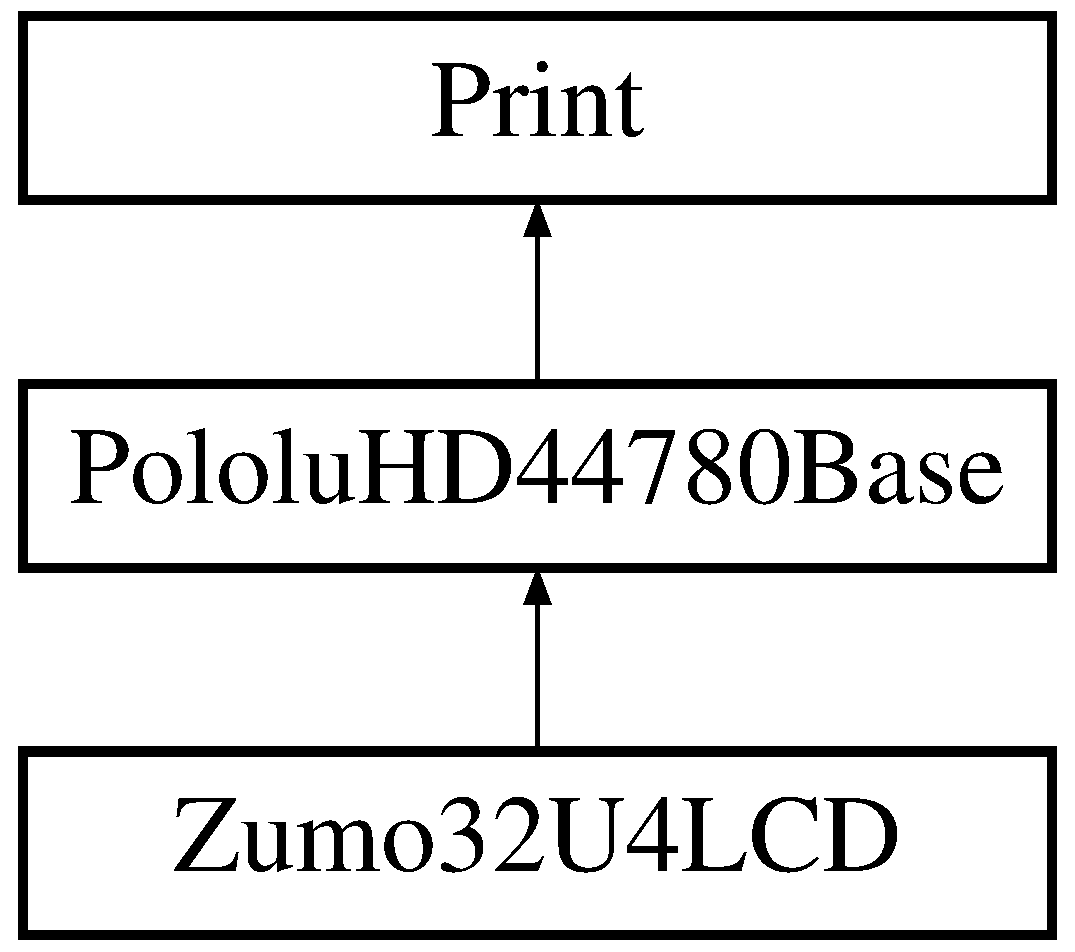
\includegraphics[height=3.000000cm]{class_zumo32_u4_l_c_d}
\end{center}
\end{figure}
\doxysubsection*{Public Member Functions}
\begin{DoxyCompactItemize}
\item 
virtual void \mbox{\hyperlink{class_zumo32_u4_l_c_d_a15ad296b2faa2196760b816301983ea5}{init\+Pins}} ()
\item 
virtual void \mbox{\hyperlink{class_zumo32_u4_l_c_d_a219e5ae0c67b8a5fd359c397c69ab713}{send}} (uint8\+\_\+t data, bool rs\+Value, bool only4bits)
\item 
void \mbox{\hyperlink{class_pololu_h_d44780_base_a1c2a3edc8cfecde7e6fd2a83c17c0e23}{init}} ()
\item 
void \mbox{\hyperlink{class_pololu_h_d44780_base_a10c1c42406708172fc38b718790ba881}{reinitialize}} ()
\item 
void \mbox{\hyperlink{class_pololu_h_d44780_base_a4d35e9a47ceef1a7582e180165e0eae1}{clear}} ()
\item 
void \mbox{\hyperlink{class_pololu_h_d44780_base_a73d331af44ec2e624aa0468ce13f64e4}{load\+Custom\+Character}} (const uint8\+\_\+t $\ast$picture, uint8\+\_\+t number)
\item 
void \mbox{\hyperlink{class_pololu_h_d44780_base_a4f22d613433fce0e0c661a237ade9aeb}{load\+Custom\+Character}} (const char $\ast$picture, uint8\+\_\+t number)
\item 
void \mbox{\hyperlink{class_pololu_h_d44780_base_a72674b5466690b49b639ae2ec3e4983f}{load\+Custom\+Character\+From\+Ram}} (const uint8\+\_\+t $\ast$picture, uint8\+\_\+t number)
\item 
void \mbox{\hyperlink{class_pololu_h_d44780_base_afd802cdc57783830acfe2415355d9f09}{create\+Char}} (uint8\+\_\+t number, uint8\+\_\+t picture\mbox{[}$\,$\mbox{]})
\item 
void \mbox{\hyperlink{class_pololu_h_d44780_base_a4886df8c888669cf71675072689ace9b}{goto\+XY}} (uint8\+\_\+t x, uint8\+\_\+t y)
\item 
void \mbox{\hyperlink{class_pololu_h_d44780_base_aeb3377822dc672398a991f06a00312c0}{set\+Cursor}} (uint8\+\_\+t col, uint8\+\_\+t row)
\item 
void \mbox{\hyperlink{class_pololu_h_d44780_base_abc2d4e126017565c2a0cf2aac67870a0}{no\+Display}} ()
\item 
void \mbox{\hyperlink{class_pololu_h_d44780_base_af5dd1e137bfe9310a418924b7483fcdf}{display}} ()
\item 
void \mbox{\hyperlink{class_pololu_h_d44780_base_ab40886cf0b563a1806bc9391d00b032d}{no\+Cursor}} ()
\item 
void \mbox{\hyperlink{class_pololu_h_d44780_base_a4fd53028d74561be579103d674aa8eab}{cursor}} ()
\item 
void \mbox{\hyperlink{class_pololu_h_d44780_base_a301afc921881052b166e11cd45ad9696}{no\+Blink}} ()
\item 
void \mbox{\hyperlink{class_pololu_h_d44780_base_ac6e255adf32d5c70c0163422b1ae8e0c}{blink}} ()
\item 
void \mbox{\hyperlink{class_pololu_h_d44780_base_a6a4d8e79beda9f7c81659a8e13c8c338}{cursor\+Solid}} ()
\item 
void \mbox{\hyperlink{class_pololu_h_d44780_base_a6a53a6cffbb77953b5a2c4ae49e288de}{cursor\+Blinking}} ()
\item 
void \mbox{\hyperlink{class_pololu_h_d44780_base_a1db083d254d251c479a577f29bcdcec8}{hide\+Cursor}} ()
\item 
void \mbox{\hyperlink{class_pololu_h_d44780_base_aada34a47663585f60b70e1d6f936f6d3}{scroll\+Display\+Left}} ()
\item 
void \mbox{\hyperlink{class_pololu_h_d44780_base_a411512707f303af75de3c5aea313bf48}{scroll\+Display\+Right}} ()
\item 
void \mbox{\hyperlink{class_pololu_h_d44780_base_ab2d24add3c6da0328055bceb38a6d42c}{home}} ()
\item 
void \mbox{\hyperlink{class_pololu_h_d44780_base_ada551bdb01681eb57bec325778eb38a6}{left\+To\+Right}} ()
\item 
void \mbox{\hyperlink{class_pololu_h_d44780_base_aa3f8d4ba18feb9aa0f0a2fef3c6c2b37}{right\+To\+Left}} ()
\item 
void \mbox{\hyperlink{class_pololu_h_d44780_base_ad5104d9651fd95704d1ae192073b0d61}{autoscroll}} ()
\item 
void \mbox{\hyperlink{class_pololu_h_d44780_base_aee80e23d270913dd2c353e7bd5408249}{no\+Autoscroll}} ()
\item 
void \mbox{\hyperlink{class_pololu_h_d44780_base_a449ad8d9ff7afb90667da0003a39af3b}{command}} (uint8\+\_\+t cmd)
\item 
virtual size\+\_\+t \mbox{\hyperlink{class_pololu_h_d44780_base_a1aad3b3ce5820dc910174b3c91a5d65e}{write}} (uint8\+\_\+t c)
\item 
virtual size\+\_\+t \mbox{\hyperlink{class_pololu_h_d44780_base_a965028ffd2313e9eaa968348effcab81}{write}} (const uint8\+\_\+t $\ast$buffer, size\+\_\+t size)
\end{DoxyCompactItemize}


\doxysubsection{Detailed Description}
Writes data to the LCD on the Zumo 32U4. 

This library is similar to the Arduino \href{http://arduino.cc/en/Reference/LiquidCrystal}{\texttt{ Liquid\+Crystal library}}, but it has some extra features needed on the Zumo 32U4\+:


\begin{DoxyItemize}
\item This class disables USB interrupts temporarily while writing to the LCD so that the USB interrupts will not change the RXLED and TXLED pins, which double as LCD data lines.
\item This class restores the RS, DB4, DB5, DB6, and DB7 pins to their previous states when it is done using them so that those pins can also be used for other purposes such as controlling LEDs.
\end{DoxyItemize}

This class inherits from the Arduino Print class, so you can call the {\ttfamily print()} function on it with a variety of arguments. See the \href{http://arduino.cc/en/Serial/Print}{\texttt{ Arduino print() documentation}} for more information.

For detailed information about HD44780 LCD interface, including what characters can be displayed, see the \href{http://www.pololu.com/file/0J72/HD44780.pdf}{\texttt{ HD44780 datasheet}}. 

Definition at line \mbox{\hyperlink{_zumo32_u4_l_c_d_8h_source_l00033}{33}} of file \mbox{\hyperlink{_zumo32_u4_l_c_d_8h_source}{Zumo32\+U4\+LCD.\+h}}.



\doxysubsection{Member Function Documentation}
\mbox{\Hypertarget{class_pololu_h_d44780_base_ad5104d9651fd95704d1ae192073b0d61}\label{class_pololu_h_d44780_base_ad5104d9651fd95704d1ae192073b0d61}} 
\index{Zumo32U4LCD@{Zumo32U4LCD}!autoscroll@{autoscroll}}
\index{autoscroll@{autoscroll}!Zumo32U4LCD@{Zumo32U4LCD}}
\doxysubsubsection{\texorpdfstring{autoscroll()}{autoscroll()}}
{\footnotesize\ttfamily void Pololu\+HD44780\+Base\+::autoscroll (\begin{DoxyParamCaption}{ }\end{DoxyParamCaption})\hspace{0.3cm}{\ttfamily [inherited]}}

Turns on auto-\/scrolling.

When auto-\/scrolling is enabled, every time a character is written, the screen will automatically scroll by one column in the appropriate direction. 

Definition at line \mbox{\hyperlink{_pololu_h_d44780_8cpp_source_l00214}{214}} of file \mbox{\hyperlink{_pololu_h_d44780_8cpp_source}{Pololu\+HD44780.\+cpp}}.

\mbox{\Hypertarget{class_pololu_h_d44780_base_ac6e255adf32d5c70c0163422b1ae8e0c}\label{class_pololu_h_d44780_base_ac6e255adf32d5c70c0163422b1ae8e0c}} 
\index{Zumo32U4LCD@{Zumo32U4LCD}!blink@{blink}}
\index{blink@{blink}!Zumo32U4LCD@{Zumo32U4LCD}}
\doxysubsubsection{\texorpdfstring{blink()}{blink()}}
{\footnotesize\ttfamily void Pololu\+HD44780\+Base\+::blink (\begin{DoxyParamCaption}{ }\end{DoxyParamCaption})\hspace{0.3cm}{\ttfamily [inherited]}}

Shows the blinking cursor.

This function sets the LCD\textquotesingle{}s \char`\"{}\+B\char`\"{} configuration bit without changing the other bits.

The cursor will normally be a blinking rectangle, but there could also be a row of solid black pixels at the bottom if previous commands have enabled the solid cursor. For this reason, it is usually better to call \mbox{\hyperlink{class_pololu_h_d44780_base_a6a4d8e79beda9f7c81659a8e13c8c338}{cursor\+Solid()}} or \mbox{\hyperlink{class_pololu_h_d44780_base_a6a53a6cffbb77953b5a2c4ae49e288de}{cursor\+Blinking()}} instead. This function is only provided for compatibilty with the Liquid\+Crystal library. 

Definition at line \mbox{\hyperlink{_pololu_h_d44780_8cpp_source_l00177}{177}} of file \mbox{\hyperlink{_pololu_h_d44780_8cpp_source}{Pololu\+HD44780.\+cpp}}.

\mbox{\Hypertarget{class_pololu_h_d44780_base_a4d35e9a47ceef1a7582e180165e0eae1}\label{class_pololu_h_d44780_base_a4d35e9a47ceef1a7582e180165e0eae1}} 
\index{Zumo32U4LCD@{Zumo32U4LCD}!clear@{clear}}
\index{clear@{clear}!Zumo32U4LCD@{Zumo32U4LCD}}
\doxysubsubsection{\texorpdfstring{clear()}{clear()}}
{\footnotesize\ttfamily void Pololu\+HD44780\+Base\+::clear (\begin{DoxyParamCaption}{ }\end{DoxyParamCaption})\hspace{0.3cm}{\ttfamily [inherited]}}

Clear the contents of the LCDs, resets the cursor position to the upper left, and resets the scroll position. 

Definition at line \mbox{\hyperlink{_pololu_h_d44780_8cpp_source_l00078}{78}} of file \mbox{\hyperlink{_pololu_h_d44780_8cpp_source}{Pololu\+HD44780.\+cpp}}.

\mbox{\Hypertarget{class_pololu_h_d44780_base_a449ad8d9ff7afb90667da0003a39af3b}\label{class_pololu_h_d44780_base_a449ad8d9ff7afb90667da0003a39af3b}} 
\index{Zumo32U4LCD@{Zumo32U4LCD}!command@{command}}
\index{command@{command}!Zumo32U4LCD@{Zumo32U4LCD}}
\doxysubsubsection{\texorpdfstring{command()}{command()}}
{\footnotesize\ttfamily void Pololu\+HD44780\+Base\+::command (\begin{DoxyParamCaption}\item[{uint8\+\_\+t}]{cmd }\end{DoxyParamCaption})\hspace{0.3cm}{\ttfamily [inline]}, {\ttfamily [inherited]}}

Send an arbitrary command to the LCD. This is here for compatibility with the Liquid\+Crystal library. 

Definition at line \mbox{\hyperlink{_pololu_h_d44780_8h_source_l00294}{294}} of file \mbox{\hyperlink{_pololu_h_d44780_8h_source}{Pololu\+HD44780.\+h}}.

\mbox{\Hypertarget{class_pololu_h_d44780_base_afd802cdc57783830acfe2415355d9f09}\label{class_pololu_h_d44780_base_afd802cdc57783830acfe2415355d9f09}} 
\index{Zumo32U4LCD@{Zumo32U4LCD}!createChar@{createChar}}
\index{createChar@{createChar}!Zumo32U4LCD@{Zumo32U4LCD}}
\doxysubsubsection{\texorpdfstring{createChar()}{createChar()}}
{\footnotesize\ttfamily void Pololu\+HD44780\+Base\+::create\+Char (\begin{DoxyParamCaption}\item[{uint8\+\_\+t}]{number,  }\item[{uint8\+\_\+t}]{picture\mbox{[}$\,$\mbox{]} }\end{DoxyParamCaption})\hspace{0.3cm}{\ttfamily [inline]}, {\ttfamily [inherited]}}

Defines a custom character. This is provided for compatibility with the Liquid\+Crystal library. 

Definition at line \mbox{\hyperlink{_pololu_h_d44780_8h_source_l00152}{152}} of file \mbox{\hyperlink{_pololu_h_d44780_8h_source}{Pololu\+HD44780.\+h}}.

\mbox{\Hypertarget{class_pololu_h_d44780_base_a4fd53028d74561be579103d674aa8eab}\label{class_pololu_h_d44780_base_a4fd53028d74561be579103d674aa8eab}} 
\index{Zumo32U4LCD@{Zumo32U4LCD}!cursor@{cursor}}
\index{cursor@{cursor}!Zumo32U4LCD@{Zumo32U4LCD}}
\doxysubsubsection{\texorpdfstring{cursor()}{cursor()}}
{\footnotesize\ttfamily void Pololu\+HD44780\+Base\+::cursor (\begin{DoxyParamCaption}{ }\end{DoxyParamCaption})\hspace{0.3cm}{\ttfamily [inherited]}}

Shows the solid cursor.

This function sets the LCD\textquotesingle{}s \char`\"{}\+C\char`\"{} configuration bit without changing the other bits.

The cursor will normally be a solid line in the bottom row, but there could be a blinking rectangle superimposed on it if previous commands have enabled the blinking cursor. For this reason, it is usually better to call \mbox{\hyperlink{class_pololu_h_d44780_base_a6a4d8e79beda9f7c81659a8e13c8c338}{cursor\+Solid()}} or \mbox{\hyperlink{class_pololu_h_d44780_base_a6a53a6cffbb77953b5a2c4ae49e288de}{cursor\+Blinking()}} instead. This function is only provided for compatibility with the Liquid\+Crystal library. 

Definition at line \mbox{\hyperlink{_pololu_h_d44780_8cpp_source_l00167}{167}} of file \mbox{\hyperlink{_pololu_h_d44780_8cpp_source}{Pololu\+HD44780.\+cpp}}.

\mbox{\Hypertarget{class_pololu_h_d44780_base_a6a53a6cffbb77953b5a2c4ae49e288de}\label{class_pololu_h_d44780_base_a6a53a6cffbb77953b5a2c4ae49e288de}} 
\index{Zumo32U4LCD@{Zumo32U4LCD}!cursorBlinking@{cursorBlinking}}
\index{cursorBlinking@{cursorBlinking}!Zumo32U4LCD@{Zumo32U4LCD}}
\doxysubsubsection{\texorpdfstring{cursorBlinking()}{cursorBlinking()}}
{\footnotesize\ttfamily void Pololu\+HD44780\+Base\+::cursor\+Blinking (\begin{DoxyParamCaption}{ }\end{DoxyParamCaption})\hspace{0.3cm}{\ttfamily [inherited]}}

Enables a cursor that appears as a blinking black rectangle.

This sets the LCD\textquotesingle{}s \char`\"{}\+C\char`\"{} and \char`\"{}\+B\char`\"{} configuration bits.

Note that the cursor will not be shown if the display is currently off (due to a call to \mbox{\hyperlink{class_pololu_h_d44780_base_abc2d4e126017565c2a0cf2aac67870a0}{no\+Display()}}), or if the cursor position is not within the bounds of the screen. 

Definition at line \mbox{\hyperlink{_pololu_h_d44780_8cpp_source_l00142}{142}} of file \mbox{\hyperlink{_pololu_h_d44780_8cpp_source}{Pololu\+HD44780.\+cpp}}.

\mbox{\Hypertarget{class_pololu_h_d44780_base_a6a4d8e79beda9f7c81659a8e13c8c338}\label{class_pololu_h_d44780_base_a6a4d8e79beda9f7c81659a8e13c8c338}} 
\index{Zumo32U4LCD@{Zumo32U4LCD}!cursorSolid@{cursorSolid}}
\index{cursorSolid@{cursorSolid}!Zumo32U4LCD@{Zumo32U4LCD}}
\doxysubsubsection{\texorpdfstring{cursorSolid()}{cursorSolid()}}
{\footnotesize\ttfamily void Pololu\+HD44780\+Base\+::cursor\+Solid (\begin{DoxyParamCaption}{ }\end{DoxyParamCaption})\hspace{0.3cm}{\ttfamily [inherited]}}

Enables a cursor that appears as a solid line in the bottom row.

This sets the LCD\textquotesingle{}s \char`\"{}\+C\char`\"{} configuration bit and clears its \char`\"{}\+B\char`\"{} bit.

Note that the cursor will not be shown if the display is currently off (due to a call to \mbox{\hyperlink{class_pololu_h_d44780_base_abc2d4e126017565c2a0cf2aac67870a0}{no\+Display()}}), or if the cursor position is not within the bounds of the screen. 

Definition at line \mbox{\hyperlink{_pololu_h_d44780_8cpp_source_l00137}{137}} of file \mbox{\hyperlink{_pololu_h_d44780_8cpp_source}{Pololu\+HD44780.\+cpp}}.

\mbox{\Hypertarget{class_pololu_h_d44780_base_af5dd1e137bfe9310a418924b7483fcdf}\label{class_pololu_h_d44780_base_af5dd1e137bfe9310a418924b7483fcdf}} 
\index{Zumo32U4LCD@{Zumo32U4LCD}!display@{display}}
\index{display@{display}!Zumo32U4LCD@{Zumo32U4LCD}}
\doxysubsubsection{\texorpdfstring{display()}{display()}}
{\footnotesize\ttfamily void Pololu\+HD44780\+Base\+::display (\begin{DoxyParamCaption}{ }\end{DoxyParamCaption})\hspace{0.3cm}{\ttfamily [inherited]}}

Turns the display on. This should only be needed if \mbox{\hyperlink{class_pololu_h_d44780_base_abc2d4e126017565c2a0cf2aac67870a0}{no\+Display()}} was previously called. 

Definition at line \mbox{\hyperlink{_pololu_h_d44780_8cpp_source_l00157}{157}} of file \mbox{\hyperlink{_pololu_h_d44780_8cpp_source}{Pololu\+HD44780.\+cpp}}.

\mbox{\Hypertarget{class_pololu_h_d44780_base_a4886df8c888669cf71675072689ace9b}\label{class_pololu_h_d44780_base_a4886df8c888669cf71675072689ace9b}} 
\index{Zumo32U4LCD@{Zumo32U4LCD}!gotoXY@{gotoXY}}
\index{gotoXY@{gotoXY}!Zumo32U4LCD@{Zumo32U4LCD}}
\doxysubsubsection{\texorpdfstring{gotoXY()}{gotoXY()}}
{\footnotesize\ttfamily void Pololu\+HD44780\+Base\+::goto\+XY (\begin{DoxyParamCaption}\item[{uint8\+\_\+t}]{x,  }\item[{uint8\+\_\+t}]{y }\end{DoxyParamCaption})\hspace{0.3cm}{\ttfamily [inherited]}}

Change the location of the cursor. The cursor (whether visible or invisible), is the place where the next character written to the LCD will be displayed.

Note that the scrolling features of the LCD change the correspondence between the {\ttfamily x} parameter and the physical column that the data is displayed on. See the \char`\"{}\+LCD scrolling\char`\"{} section above for more information.


\begin{DoxyParams}{Parameters}
{\em x} & The number of the column to go to, with 0 being the leftmost column. \\
\hline
{\em y} & The number of the row to go to, with 0 being the top row. \\
\hline
\end{DoxyParams}


Definition at line \mbox{\hyperlink{_pololu_h_d44780_8cpp_source_l00088}{88}} of file \mbox{\hyperlink{_pololu_h_d44780_8cpp_source}{Pololu\+HD44780.\+cpp}}.

\mbox{\Hypertarget{class_pololu_h_d44780_base_a1db083d254d251c479a577f29bcdcec8}\label{class_pololu_h_d44780_base_a1db083d254d251c479a577f29bcdcec8}} 
\index{Zumo32U4LCD@{Zumo32U4LCD}!hideCursor@{hideCursor}}
\index{hideCursor@{hideCursor}!Zumo32U4LCD@{Zumo32U4LCD}}
\doxysubsubsection{\texorpdfstring{hideCursor()}{hideCursor()}}
{\footnotesize\ttfamily void Pololu\+HD44780\+Base\+::hide\+Cursor (\begin{DoxyParamCaption}{ }\end{DoxyParamCaption})\hspace{0.3cm}{\ttfamily [inherited]}}

Hides the solid and blinking cursors.

This clears the LCD\textquotesingle{}s \char`\"{}\+C\char`\"{} and \char`\"{}\+B\char`\"{} configuration bits. 

Definition at line \mbox{\hyperlink{_pololu_h_d44780_8cpp_source_l00147}{147}} of file \mbox{\hyperlink{_pololu_h_d44780_8cpp_source}{Pololu\+HD44780.\+cpp}}.

\mbox{\Hypertarget{class_pololu_h_d44780_base_ab2d24add3c6da0328055bceb38a6d42c}\label{class_pololu_h_d44780_base_ab2d24add3c6da0328055bceb38a6d42c}} 
\index{Zumo32U4LCD@{Zumo32U4LCD}!home@{home}}
\index{home@{home}!Zumo32U4LCD@{Zumo32U4LCD}}
\doxysubsubsection{\texorpdfstring{home()}{home()}}
{\footnotesize\ttfamily void Pololu\+HD44780\+Base\+::home (\begin{DoxyParamCaption}{ }\end{DoxyParamCaption})\hspace{0.3cm}{\ttfamily [inherited]}}

Resets the screen scrolling position back to the default and moves the cursor to the upper left corner of the screen.

This command takes about 1600 microseconds, so it would be faster to instead call \mbox{\hyperlink{class_pololu_h_d44780_base_aada34a47663585f60b70e1d6f936f6d3}{scroll\+Display\+Left()}} or \mbox{\hyperlink{class_pololu_h_d44780_base_a411512707f303af75de3c5aea313bf48}{scroll\+Display\+Right()}} the appropriate number of times and then call goto\+XY(0, 0). 

Definition at line \mbox{\hyperlink{_pololu_h_d44780_8cpp_source_l00192}{192}} of file \mbox{\hyperlink{_pololu_h_d44780_8cpp_source}{Pololu\+HD44780.\+cpp}}.

\mbox{\Hypertarget{class_pololu_h_d44780_base_a1c2a3edc8cfecde7e6fd2a83c17c0e23}\label{class_pololu_h_d44780_base_a1c2a3edc8cfecde7e6fd2a83c17c0e23}} 
\index{Zumo32U4LCD@{Zumo32U4LCD}!init@{init}}
\index{init@{init}!Zumo32U4LCD@{Zumo32U4LCD}}
\doxysubsubsection{\texorpdfstring{init()}{init()}}
{\footnotesize\ttfamily void Pololu\+HD44780\+Base\+::init (\begin{DoxyParamCaption}{ }\end{DoxyParamCaption})\hspace{0.3cm}{\ttfamily [inline]}, {\ttfamily [inherited]}}

Initialize the LCD if it has not already been initialized. 

Definition at line \mbox{\hyperlink{_pololu_h_d44780_8h_source_l00067}{67}} of file \mbox{\hyperlink{_pololu_h_d44780_8h_source}{Pololu\+HD44780.\+h}}.

\mbox{\Hypertarget{class_zumo32_u4_l_c_d_a15ad296b2faa2196760b816301983ea5}\label{class_zumo32_u4_l_c_d_a15ad296b2faa2196760b816301983ea5}} 
\index{Zumo32U4LCD@{Zumo32U4LCD}!initPins@{initPins}}
\index{initPins@{initPins}!Zumo32U4LCD@{Zumo32U4LCD}}
\doxysubsubsection{\texorpdfstring{initPins()}{initPins()}}
{\footnotesize\ttfamily virtual void Zumo32\+U4\+LCD\+::init\+Pins (\begin{DoxyParamCaption}{ }\end{DoxyParamCaption})\hspace{0.3cm}{\ttfamily [inline]}, {\ttfamily [virtual]}}

Initializes the pins so that the \mbox{\hyperlink{class_zumo32_u4_l_c_d_a219e5ae0c67b8a5fd359c397c69ab713}{send()}} function can be called successfully. This is the first step of initializing the LCD. 

Implements \mbox{\hyperlink{class_pololu_h_d44780_base_a9c2a2e0dfb089a6c21aa12a6a5299750}{Pololu\+HD44780\+Base}}.



Definition at line \mbox{\hyperlink{_zumo32_u4_l_c_d_8h_source_l00040}{40}} of file \mbox{\hyperlink{_zumo32_u4_l_c_d_8h_source}{Zumo32\+U4\+LCD.\+h}}.

\mbox{\Hypertarget{class_pololu_h_d44780_base_ada551bdb01681eb57bec325778eb38a6}\label{class_pololu_h_d44780_base_ada551bdb01681eb57bec325778eb38a6}} 
\index{Zumo32U4LCD@{Zumo32U4LCD}!leftToRight@{leftToRight}}
\index{leftToRight@{leftToRight}!Zumo32U4LCD@{Zumo32U4LCD}}
\doxysubsubsection{\texorpdfstring{leftToRight()}{leftToRight()}}
{\footnotesize\ttfamily void Pololu\+HD44780\+Base\+::left\+To\+Right (\begin{DoxyParamCaption}{ }\end{DoxyParamCaption})\hspace{0.3cm}{\ttfamily [inherited]}}

Puts the LCD into left-\/to-\/right mode\+: the cursor will shift to the right after any character is written. This is the default behavior. 

Definition at line \mbox{\hyperlink{_pololu_h_d44780_8cpp_source_l00204}{204}} of file \mbox{\hyperlink{_pololu_h_d44780_8cpp_source}{Pololu\+HD44780.\+cpp}}.

\mbox{\Hypertarget{class_pololu_h_d44780_base_a4f22d613433fce0e0c661a237ade9aeb}\label{class_pololu_h_d44780_base_a4f22d613433fce0e0c661a237ade9aeb}} 
\index{Zumo32U4LCD@{Zumo32U4LCD}!loadCustomCharacter@{loadCustomCharacter}}
\index{loadCustomCharacter@{loadCustomCharacter}!Zumo32U4LCD@{Zumo32U4LCD}}
\doxysubsubsection{\texorpdfstring{loadCustomCharacter()}{loadCustomCharacter()}\hspace{0.1cm}{\footnotesize\ttfamily [1/2]}}
{\footnotesize\ttfamily void Pololu\+HD44780\+Base\+::load\+Custom\+Character (\begin{DoxyParamCaption}\item[{const char $\ast$}]{picture,  }\item[{uint8\+\_\+t}]{number }\end{DoxyParamCaption})\hspace{0.3cm}{\ttfamily [inline]}, {\ttfamily [inherited]}}

This overload of load\+Custom\+Character is only provided for compatibility with Orangutan\+LCD; a lot of Orangutan code defines an array of chars for custom character pictures. 

Definition at line \mbox{\hyperlink{_pololu_h_d44780_8h_source_l00145}{145}} of file \mbox{\hyperlink{_pololu_h_d44780_8h_source}{Pololu\+HD44780.\+h}}.

\mbox{\Hypertarget{class_pololu_h_d44780_base_a73d331af44ec2e624aa0468ce13f64e4}\label{class_pololu_h_d44780_base_a73d331af44ec2e624aa0468ce13f64e4}} 
\index{Zumo32U4LCD@{Zumo32U4LCD}!loadCustomCharacter@{loadCustomCharacter}}
\index{loadCustomCharacter@{loadCustomCharacter}!Zumo32U4LCD@{Zumo32U4LCD}}
\doxysubsubsection{\texorpdfstring{loadCustomCharacter()}{loadCustomCharacter()}\hspace{0.1cm}{\footnotesize\ttfamily [2/2]}}
{\footnotesize\ttfamily void Pololu\+HD44780\+Base\+::load\+Custom\+Character (\begin{DoxyParamCaption}\item[{const uint8\+\_\+t $\ast$}]{picture,  }\item[{uint8\+\_\+t}]{number }\end{DoxyParamCaption})\hspace{0.3cm}{\ttfamily [inherited]}}

Defines a custom character. 
\begin{DoxyParams}{Parameters}
{\em picture} & A pointer to the character dot pattern, in program space. \\
\hline
{\em number} & A number between 0 and 7. \\
\hline
\end{DoxyParams}


Definition at line \mbox{\hyperlink{_pololu_h_d44780_8cpp_source_l00103}{103}} of file \mbox{\hyperlink{_pololu_h_d44780_8cpp_source}{Pololu\+HD44780.\+cpp}}.

\mbox{\Hypertarget{class_pololu_h_d44780_base_a72674b5466690b49b639ae2ec3e4983f}\label{class_pololu_h_d44780_base_a72674b5466690b49b639ae2ec3e4983f}} 
\index{Zumo32U4LCD@{Zumo32U4LCD}!loadCustomCharacterFromRam@{loadCustomCharacterFromRam}}
\index{loadCustomCharacterFromRam@{loadCustomCharacterFromRam}!Zumo32U4LCD@{Zumo32U4LCD}}
\doxysubsubsection{\texorpdfstring{loadCustomCharacterFromRam()}{loadCustomCharacterFromRam()}}
{\footnotesize\ttfamily void Pololu\+HD44780\+Base\+::load\+Custom\+Character\+From\+Ram (\begin{DoxyParamCaption}\item[{const uint8\+\_\+t $\ast$}]{picture,  }\item[{uint8\+\_\+t}]{number }\end{DoxyParamCaption})\hspace{0.3cm}{\ttfamily [inherited]}}

Defines a custom character from RAM. 
\begin{DoxyParams}{Parameters}
{\em picture} & A pointer to the character dot pattern, in RAM. \\
\hline
{\em number} & A number between 0 and 7. \\
\hline
\end{DoxyParams}


Definition at line \mbox{\hyperlink{_pololu_h_d44780_8cpp_source_l00117}{117}} of file \mbox{\hyperlink{_pololu_h_d44780_8cpp_source}{Pololu\+HD44780.\+cpp}}.

\mbox{\Hypertarget{class_pololu_h_d44780_base_aee80e23d270913dd2c353e7bd5408249}\label{class_pololu_h_d44780_base_aee80e23d270913dd2c353e7bd5408249}} 
\index{Zumo32U4LCD@{Zumo32U4LCD}!noAutoscroll@{noAutoscroll}}
\index{noAutoscroll@{noAutoscroll}!Zumo32U4LCD@{Zumo32U4LCD}}
\doxysubsubsection{\texorpdfstring{noAutoscroll()}{noAutoscroll()}}
{\footnotesize\ttfamily void Pololu\+HD44780\+Base\+::no\+Autoscroll (\begin{DoxyParamCaption}{ }\end{DoxyParamCaption})\hspace{0.3cm}{\ttfamily [inherited]}}

Turns off auto-\/scrolling. Auto-\/scrolling is off by default. 

Definition at line \mbox{\hyperlink{_pololu_h_d44780_8cpp_source_l00219}{219}} of file \mbox{\hyperlink{_pololu_h_d44780_8cpp_source}{Pololu\+HD44780.\+cpp}}.

\mbox{\Hypertarget{class_pololu_h_d44780_base_a301afc921881052b166e11cd45ad9696}\label{class_pololu_h_d44780_base_a301afc921881052b166e11cd45ad9696}} 
\index{Zumo32U4LCD@{Zumo32U4LCD}!noBlink@{noBlink}}
\index{noBlink@{noBlink}!Zumo32U4LCD@{Zumo32U4LCD}}
\doxysubsubsection{\texorpdfstring{noBlink()}{noBlink()}}
{\footnotesize\ttfamily void Pololu\+HD44780\+Base\+::no\+Blink (\begin{DoxyParamCaption}{ }\end{DoxyParamCaption})\hspace{0.3cm}{\ttfamily [inherited]}}

Hides the blinking cursor.

This functions clears the LCD\textquotesingle{}s \char`\"{}\+B\char`\"{} configuration bit without changing the other bits.

Calling this function does not enable or disable the solid cursor (a solid line in the bottom row) so it is usually better to call \mbox{\hyperlink{class_pololu_h_d44780_base_a1db083d254d251c479a577f29bcdcec8}{hide\+Cursor()}} or \mbox{\hyperlink{class_pololu_h_d44780_base_a6a4d8e79beda9f7c81659a8e13c8c338}{cursor\+Solid()}} instead. This function is only provided for compatibilty with the Liquid\+Crystal library. 

Definition at line \mbox{\hyperlink{_pololu_h_d44780_8cpp_source_l00172}{172}} of file \mbox{\hyperlink{_pololu_h_d44780_8cpp_source}{Pololu\+HD44780.\+cpp}}.

\mbox{\Hypertarget{class_pololu_h_d44780_base_ab40886cf0b563a1806bc9391d00b032d}\label{class_pololu_h_d44780_base_ab40886cf0b563a1806bc9391d00b032d}} 
\index{Zumo32U4LCD@{Zumo32U4LCD}!noCursor@{noCursor}}
\index{noCursor@{noCursor}!Zumo32U4LCD@{Zumo32U4LCD}}
\doxysubsubsection{\texorpdfstring{noCursor()}{noCursor()}}
{\footnotesize\ttfamily void Pololu\+HD44780\+Base\+::no\+Cursor (\begin{DoxyParamCaption}{ }\end{DoxyParamCaption})\hspace{0.3cm}{\ttfamily [inherited]}}

Hides the solid cursor.

This function clears the LCD\textquotesingle{}s \char`\"{}\+C\char`\"{} configuration bit without changing the other bits.

If the \char`\"{}\+B\char`\"{} bit is set to 1, a blinking cursor will still be displayed even after calling this function. For that reason, it is usually better to call \mbox{\hyperlink{class_pololu_h_d44780_base_a1db083d254d251c479a577f29bcdcec8}{hide\+Cursor()}} instead. This function is only provided for compatibility with the Liquid\+Crystal library. 

Definition at line \mbox{\hyperlink{_pololu_h_d44780_8cpp_source_l00162}{162}} of file \mbox{\hyperlink{_pololu_h_d44780_8cpp_source}{Pololu\+HD44780.\+cpp}}.

\mbox{\Hypertarget{class_pololu_h_d44780_base_abc2d4e126017565c2a0cf2aac67870a0}\label{class_pololu_h_d44780_base_abc2d4e126017565c2a0cf2aac67870a0}} 
\index{Zumo32U4LCD@{Zumo32U4LCD}!noDisplay@{noDisplay}}
\index{noDisplay@{noDisplay}!Zumo32U4LCD@{Zumo32U4LCD}}
\doxysubsubsection{\texorpdfstring{noDisplay()}{noDisplay()}}
{\footnotesize\ttfamily void Pololu\+HD44780\+Base\+::no\+Display (\begin{DoxyParamCaption}{ }\end{DoxyParamCaption})\hspace{0.3cm}{\ttfamily [inherited]}}

Turns off the display while preserving its state.

You can turn the display on again by calling \mbox{\hyperlink{class_pololu_h_d44780_base_af5dd1e137bfe9310a418924b7483fcdf}{display()}}. 

Definition at line \mbox{\hyperlink{_pololu_h_d44780_8cpp_source_l00152}{152}} of file \mbox{\hyperlink{_pololu_h_d44780_8cpp_source}{Pololu\+HD44780.\+cpp}}.

\mbox{\Hypertarget{class_pololu_h_d44780_base_a10c1c42406708172fc38b718790ba881}\label{class_pololu_h_d44780_base_a10c1c42406708172fc38b718790ba881}} 
\index{Zumo32U4LCD@{Zumo32U4LCD}!reinitialize@{reinitialize}}
\index{reinitialize@{reinitialize}!Zumo32U4LCD@{Zumo32U4LCD}}
\doxysubsubsection{\texorpdfstring{reinitialize()}{reinitialize()}}
{\footnotesize\ttfamily void Pololu\+HD44780\+Base\+::reinitialize (\begin{DoxyParamCaption}{ }\end{DoxyParamCaption})\hspace{0.3cm}{\ttfamily [inline]}, {\ttfamily [inherited]}}

Reinitialize the LCD. This performs the same initialization that is done automatically the first time any function is called that writes to the LCD. This is useful if you want to get it back to a totally clean state. 

Definition at line \mbox{\hyperlink{_pololu_h_d44780_8h_source_l00080}{80}} of file \mbox{\hyperlink{_pololu_h_d44780_8h_source}{Pololu\+HD44780.\+h}}.

\mbox{\Hypertarget{class_pololu_h_d44780_base_aa3f8d4ba18feb9aa0f0a2fef3c6c2b37}\label{class_pololu_h_d44780_base_aa3f8d4ba18feb9aa0f0a2fef3c6c2b37}} 
\index{Zumo32U4LCD@{Zumo32U4LCD}!rightToLeft@{rightToLeft}}
\index{rightToLeft@{rightToLeft}!Zumo32U4LCD@{Zumo32U4LCD}}
\doxysubsubsection{\texorpdfstring{rightToLeft()}{rightToLeft()}}
{\footnotesize\ttfamily void Pololu\+HD44780\+Base\+::right\+To\+Left (\begin{DoxyParamCaption}{ }\end{DoxyParamCaption})\hspace{0.3cm}{\ttfamily [inherited]}}

Puts the LCD into right-\/to-\/left mode\+: the cursor will shift to the left after any character is written. 

Definition at line \mbox{\hyperlink{_pololu_h_d44780_8cpp_source_l00209}{209}} of file \mbox{\hyperlink{_pololu_h_d44780_8cpp_source}{Pololu\+HD44780.\+cpp}}.

\mbox{\Hypertarget{class_pololu_h_d44780_base_aada34a47663585f60b70e1d6f936f6d3}\label{class_pololu_h_d44780_base_aada34a47663585f60b70e1d6f936f6d3}} 
\index{Zumo32U4LCD@{Zumo32U4LCD}!scrollDisplayLeft@{scrollDisplayLeft}}
\index{scrollDisplayLeft@{scrollDisplayLeft}!Zumo32U4LCD@{Zumo32U4LCD}}
\doxysubsubsection{\texorpdfstring{scrollDisplayLeft()}{scrollDisplayLeft()}}
{\footnotesize\ttfamily void Pololu\+HD44780\+Base\+::scroll\+Display\+Left (\begin{DoxyParamCaption}{ }\end{DoxyParamCaption})\hspace{0.3cm}{\ttfamily [inherited]}}

Scrolls everything on the screen one position to the left.

This command takes about 37 microseconds. 

Definition at line \mbox{\hyperlink{_pololu_h_d44780_8cpp_source_l00182}{182}} of file \mbox{\hyperlink{_pololu_h_d44780_8cpp_source}{Pololu\+HD44780.\+cpp}}.

\mbox{\Hypertarget{class_pololu_h_d44780_base_a411512707f303af75de3c5aea313bf48}\label{class_pololu_h_d44780_base_a411512707f303af75de3c5aea313bf48}} 
\index{Zumo32U4LCD@{Zumo32U4LCD}!scrollDisplayRight@{scrollDisplayRight}}
\index{scrollDisplayRight@{scrollDisplayRight}!Zumo32U4LCD@{Zumo32U4LCD}}
\doxysubsubsection{\texorpdfstring{scrollDisplayRight()}{scrollDisplayRight()}}
{\footnotesize\ttfamily void Pololu\+HD44780\+Base\+::scroll\+Display\+Right (\begin{DoxyParamCaption}{ }\end{DoxyParamCaption})\hspace{0.3cm}{\ttfamily [inherited]}}

Scrolls everything on the screen one position to the right.

This command takes about 37 microseconds. 

Definition at line \mbox{\hyperlink{_pololu_h_d44780_8cpp_source_l00187}{187}} of file \mbox{\hyperlink{_pololu_h_d44780_8cpp_source}{Pololu\+HD44780.\+cpp}}.

\mbox{\Hypertarget{class_zumo32_u4_l_c_d_a219e5ae0c67b8a5fd359c397c69ab713}\label{class_zumo32_u4_l_c_d_a219e5ae0c67b8a5fd359c397c69ab713}} 
\index{Zumo32U4LCD@{Zumo32U4LCD}!send@{send}}
\index{send@{send}!Zumo32U4LCD@{Zumo32U4LCD}}
\doxysubsubsection{\texorpdfstring{send()}{send()}}
{\footnotesize\ttfamily virtual void Zumo32\+U4\+LCD\+::send (\begin{DoxyParamCaption}\item[{uint8\+\_\+t}]{data,  }\item[{bool}]{rs\+Value,  }\item[{bool}]{only4bits }\end{DoxyParamCaption})\hspace{0.3cm}{\ttfamily [inline]}, {\ttfamily [virtual]}}

Sends data or commands to the LCD.

The \mbox{\hyperlink{class_zumo32_u4_l_c_d_a15ad296b2faa2196760b816301983ea5}{init\+Pins()}} function will always be called before the first time this function is called. This function does not need to worry about the delays necessary to make sure the previous command has finished; that is taken care of by \mbox{\hyperlink{class_pololu_h_d44780_base}{Pololu\+HD44780\+Base}}.

This function, along with \mbox{\hyperlink{class_zumo32_u4_l_c_d_a15ad296b2faa2196760b816301983ea5}{init\+Pins()}}, comprise the hardware abstraction layer for the LCD, and must be defined in a subclass of \mbox{\hyperlink{class_pololu_h_d44780_base}{Pololu\+HD44780\+Base}}. All other functions use these two functions to communicate with the LCD.


\begin{DoxyParams}{Parameters}
{\em data} & The data to send to the LCD. \\
\hline
{\em rs\+Value} & True to drive the RS pin high, false to drive it low. \\
\hline
{\em only4bits} & If true, and the LCD is using a 4-\/bit interface, only sends the lower 4 bits of the data. \\
\hline
\end{DoxyParams}


Implements \mbox{\hyperlink{class_pololu_h_d44780_base_a004d5adb9e7c3cc546c6b0ed427dec7b}{Pololu\+HD44780\+Base}}.



Definition at line \mbox{\hyperlink{_zumo32_u4_l_c_d_8h_source_l00045}{45}} of file \mbox{\hyperlink{_zumo32_u4_l_c_d_8h_source}{Zumo32\+U4\+LCD.\+h}}.

\mbox{\Hypertarget{class_pololu_h_d44780_base_aeb3377822dc672398a991f06a00312c0}\label{class_pololu_h_d44780_base_aeb3377822dc672398a991f06a00312c0}} 
\index{Zumo32U4LCD@{Zumo32U4LCD}!setCursor@{setCursor}}
\index{setCursor@{setCursor}!Zumo32U4LCD@{Zumo32U4LCD}}
\doxysubsubsection{\texorpdfstring{setCursor()}{setCursor()}}
{\footnotesize\ttfamily void Pololu\+HD44780\+Base\+::set\+Cursor (\begin{DoxyParamCaption}\item[{uint8\+\_\+t}]{col,  }\item[{uint8\+\_\+t}]{row }\end{DoxyParamCaption})\hspace{0.3cm}{\ttfamily [inline]}, {\ttfamily [inherited]}}

Changes the location of the cursor. This is just a wrapper around goto\+XY provided for compaitibility with the Liquid\+Crystal library. 

Definition at line \mbox{\hyperlink{_pololu_h_d44780_8h_source_l00170}{170}} of file \mbox{\hyperlink{_pololu_h_d44780_8h_source}{Pololu\+HD44780.\+h}}.

\mbox{\Hypertarget{class_pololu_h_d44780_base_a965028ffd2313e9eaa968348effcab81}\label{class_pololu_h_d44780_base_a965028ffd2313e9eaa968348effcab81}} 
\index{Zumo32U4LCD@{Zumo32U4LCD}!write@{write}}
\index{write@{write}!Zumo32U4LCD@{Zumo32U4LCD}}
\doxysubsubsection{\texorpdfstring{write()}{write()}\hspace{0.1cm}{\footnotesize\ttfamily [1/2]}}
{\footnotesize\ttfamily size\+\_\+t Pololu\+HD44780\+Base\+::write (\begin{DoxyParamCaption}\item[{const uint8\+\_\+t $\ast$}]{buffer,  }\item[{size\+\_\+t}]{size }\end{DoxyParamCaption})\hspace{0.3cm}{\ttfamily [virtual]}, {\ttfamily [inherited]}}

Writes multiple characters to the LCD.


\begin{DoxyParams}{Parameters}
{\em buffer} & Pointer to a string of characters in RAM, not necessarily null-\/terminated. \\
\hline
{\em size} & The number of characters to write to the LCD, excluding any null termination character. \\
\hline
\end{DoxyParams}


Definition at line \mbox{\hyperlink{_pololu_h_d44780_8cpp_source_l00068}{68}} of file \mbox{\hyperlink{_pololu_h_d44780_8cpp_source}{Pololu\+HD44780.\+cpp}}.

\mbox{\Hypertarget{class_pololu_h_d44780_base_a1aad3b3ce5820dc910174b3c91a5d65e}\label{class_pololu_h_d44780_base_a1aad3b3ce5820dc910174b3c91a5d65e}} 
\index{Zumo32U4LCD@{Zumo32U4LCD}!write@{write}}
\index{write@{write}!Zumo32U4LCD@{Zumo32U4LCD}}
\doxysubsubsection{\texorpdfstring{write()}{write()}\hspace{0.1cm}{\footnotesize\ttfamily [2/2]}}
{\footnotesize\ttfamily size\+\_\+t Pololu\+HD44780\+Base\+::write (\begin{DoxyParamCaption}\item[{uint8\+\_\+t}]{c }\end{DoxyParamCaption})\hspace{0.3cm}{\ttfamily [virtual]}, {\ttfamily [inherited]}}

Writes a single character to the LCD. 

Definition at line \mbox{\hyperlink{_pololu_h_d44780_8cpp_source_l00062}{62}} of file \mbox{\hyperlink{_pololu_h_d44780_8cpp_source}{Pololu\+HD44780.\+cpp}}.



The documentation for this class was generated from the following file\+:\begin{DoxyCompactItemize}
\item 
\mbox{\hyperlink{_zumo32_u4_l_c_d_8h}{Zumo32\+U4\+LCD.\+h}}\end{DoxyCompactItemize}

\hypertarget{class_zumo32_u4_line_sensors}{}\section{Zumo32\+U4\+Line\+Sensors Class Reference}
\label{class_zumo32_u4_line_sensors}\index{Zumo32\+U4\+Line\+Sensors@{Zumo32\+U4\+Line\+Sensors}}


Gets readings from the five down-\/facing line sensors on the front sensor array.  




{\ttfamily \#include $<$Zumo32\+U4\+Line\+Sensors.\+h$>$}

Inheritance diagram for Zumo32\+U4\+Line\+Sensors\+:\begin{figure}[H]
\begin{center}
\leavevmode
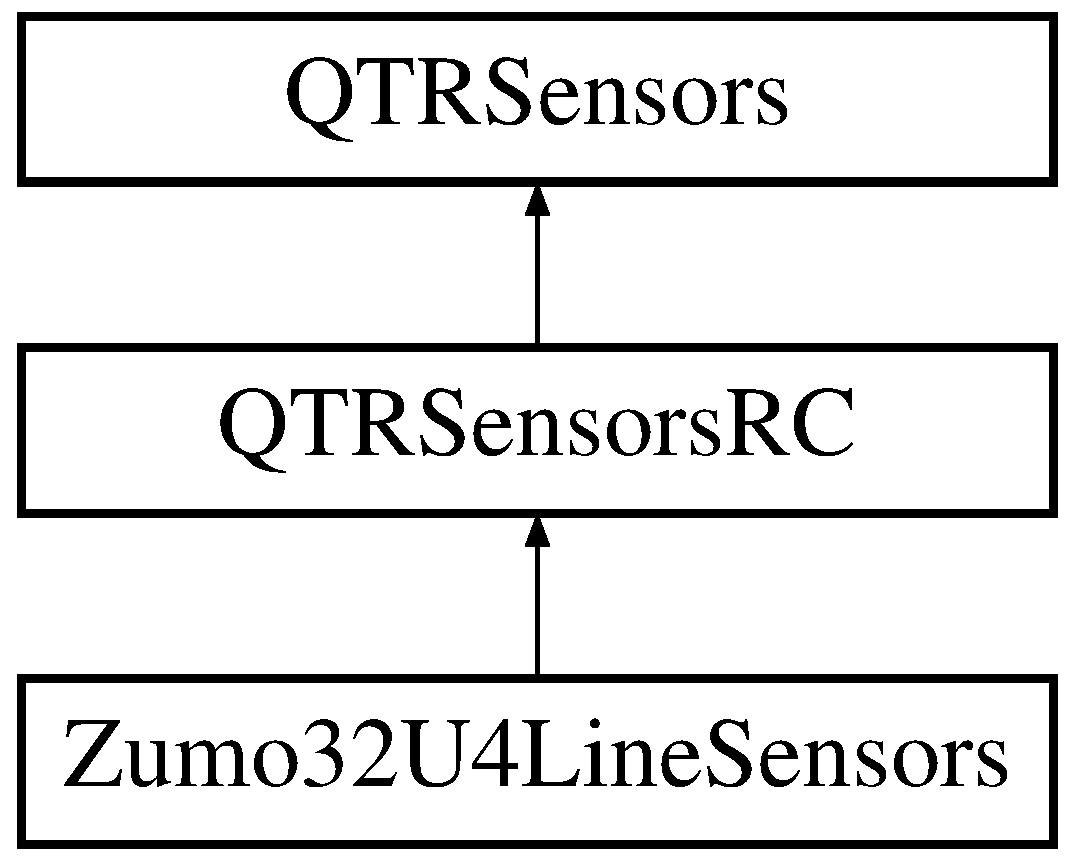
\includegraphics[height=3.000000cm]{class_zumo32_u4_line_sensors}
\end{center}
\end{figure}
\subsection*{Public Member Functions}
\begin{DoxyCompactItemize}
\item 
\hyperlink{class_zumo32_u4_line_sensors_af1e61e6f4e14544054712689d23a974d}{Zumo32\+U4\+Line\+Sensors} ()
\begin{DoxyCompactList}\small\item\em Minimal constructor. \end{DoxyCompactList}\item 
\hyperlink{class_zumo32_u4_line_sensors_a59ecf283662fbcb2993d74fd436b0e53}{Zumo32\+U4\+Line\+Sensors} (uint8\+\_\+t $\ast$pins, uint8\+\_\+t num\+Sensors, uint8\+\_\+t emitter\+Pin=\hyperlink{_zumo32_u4_line_sensors_8h_a661904c7fa6e0b2cb9645e2ef272cfcd}{S\+E\+N\+S\+O\+R\+\_\+\+L\+E\+D\+ON})
\begin{DoxyCompactList}\small\item\em Constructor that takes pin arguments. \end{DoxyCompactList}\item 
void \hyperlink{class_zumo32_u4_line_sensors_a880737a0df457e9acf3277b2342e4087}{init\+Three\+Sensors} (uint8\+\_\+t emitter\+Pin=\hyperlink{_zumo32_u4_line_sensors_8h_a661904c7fa6e0b2cb9645e2ef272cfcd}{S\+E\+N\+S\+O\+R\+\_\+\+L\+E\+D\+ON})
\begin{DoxyCompactList}\small\item\em Configures this object to use just three line sensors. \end{DoxyCompactList}\item 
void \hyperlink{class_zumo32_u4_line_sensors_a3873997ed35fbc1c6c57411f6cee1f2d}{init\+Five\+Sensors} (uint8\+\_\+t emitter\+Pin=\hyperlink{_zumo32_u4_line_sensors_8h_a661904c7fa6e0b2cb9645e2ef272cfcd}{S\+E\+N\+S\+O\+R\+\_\+\+L\+E\+D\+ON})
\begin{DoxyCompactList}\small\item\em Configures this object to use all five line sensors. \end{DoxyCompactList}\item 
void \hyperlink{class_zumo32_u4_line_sensors_aa8656b7a8c3d27302d76431acb93c2ac}{init} (uint8\+\_\+t $\ast$pins, uint8\+\_\+t num\+Sensors, uint16\+\_\+t timeout=2000, uint8\+\_\+t emitter\+Pin=\hyperlink{_zumo32_u4_line_sensors_8h_a661904c7fa6e0b2cb9645e2ef272cfcd}{S\+E\+N\+S\+O\+R\+\_\+\+L\+E\+D\+ON})
\begin{DoxyCompactList}\small\item\em Configures this object to use a custom set of pins. \end{DoxyCompactList}\item 
\mbox{\Hypertarget{class_q_t_r_sensors_r_c_a354e7064c224b6fb363405016cdf73fa}\label{class_q_t_r_sensors_r_c_a354e7064c224b6fb363405016cdf73fa}} 
void {\bfseries init} (unsigned char $\ast$pins, unsigned char num\+Sensors, unsigned int timeout=2000, unsigned char emitter\+Pin=Q\+T\+R\+\_\+\+N\+O\+\_\+\+E\+M\+I\+T\+T\+E\+R\+\_\+\+P\+IN)
\item 
\mbox{\Hypertarget{class_q_t_r_sensors_afc47e6c2608293a610e1a3acce93628b}\label{class_q_t_r_sensors_afc47e6c2608293a610e1a3acce93628b}} 
void {\bfseries read} (unsigned int $\ast$sensor\+\_\+values, unsigned char read\+Mode=Q\+T\+R\+\_\+\+E\+M\+I\+T\+T\+E\+R\+S\+\_\+\+ON)
\item 
\mbox{\Hypertarget{class_q_t_r_sensors_a576f1fe1e9f2d3d2097baf79a9655134}\label{class_q_t_r_sensors_a576f1fe1e9f2d3d2097baf79a9655134}} 
void {\bfseries emitters\+Off} ()
\item 
\mbox{\Hypertarget{class_q_t_r_sensors_a79f5380ecdb324a7800a045c3506975f}\label{class_q_t_r_sensors_a79f5380ecdb324a7800a045c3506975f}} 
void {\bfseries emitters\+On} ()
\item 
\mbox{\Hypertarget{class_q_t_r_sensors_ac9840e2429c7a962977057ba154c77da}\label{class_q_t_r_sensors_ac9840e2429c7a962977057ba154c77da}} 
void {\bfseries calibrate} (unsigned char read\+Mode=Q\+T\+R\+\_\+\+E\+M\+I\+T\+T\+E\+R\+S\+\_\+\+ON)
\item 
\mbox{\Hypertarget{class_q_t_r_sensors_aa840b6ef17562d41edf21ddd08e0672e}\label{class_q_t_r_sensors_aa840b6ef17562d41edf21ddd08e0672e}} 
void {\bfseries reset\+Calibration} ()
\item 
\mbox{\Hypertarget{class_q_t_r_sensors_aa32a448ac03cd2a45d1f14f96ac4b739}\label{class_q_t_r_sensors_aa32a448ac03cd2a45d1f14f96ac4b739}} 
void {\bfseries read\+Calibrated} (unsigned int $\ast$sensor\+\_\+values, unsigned char read\+Mode=Q\+T\+R\+\_\+\+E\+M\+I\+T\+T\+E\+R\+S\+\_\+\+ON)
\item 
\mbox{\Hypertarget{class_q_t_r_sensors_ac84f0b98bceae0b59d687ae82eb92718}\label{class_q_t_r_sensors_ac84f0b98bceae0b59d687ae82eb92718}} 
int {\bfseries read\+Line} (unsigned int $\ast$sensor\+\_\+values, unsigned char read\+Mode=Q\+T\+R\+\_\+\+E\+M\+I\+T\+T\+E\+R\+S\+\_\+\+ON, unsigned char white\+\_\+line=0)
\end{DoxyCompactItemize}
\subsection*{Public Attributes}
\begin{DoxyCompactItemize}
\item 
\mbox{\Hypertarget{class_q_t_r_sensors_a9308c21df0015965dceb9dd1f570f78d}\label{class_q_t_r_sensors_a9308c21df0015965dceb9dd1f570f78d}} 
unsigned int $\ast$ {\bfseries calibrated\+Minimum\+On}
\item 
\mbox{\Hypertarget{class_q_t_r_sensors_ab7a739d5bb85b17e94e825454cc63195}\label{class_q_t_r_sensors_ab7a739d5bb85b17e94e825454cc63195}} 
unsigned int $\ast$ {\bfseries calibrated\+Maximum\+On}
\item 
\mbox{\Hypertarget{class_q_t_r_sensors_af299d7e4a7900f4f3d5e567a10f4ab16}\label{class_q_t_r_sensors_af299d7e4a7900f4f3d5e567a10f4ab16}} 
unsigned int $\ast$ {\bfseries calibrated\+Minimum\+Off}
\item 
\mbox{\Hypertarget{class_q_t_r_sensors_a75af08628235c3ec5d4414a6032a016c}\label{class_q_t_r_sensors_a75af08628235c3ec5d4414a6032a016c}} 
unsigned int $\ast$ {\bfseries calibrated\+Maximum\+Off}
\end{DoxyCompactItemize}
\subsection*{Protected Member Functions}
\begin{DoxyCompactItemize}
\item 
\mbox{\Hypertarget{class_q_t_r_sensors_ae1d5eb9479d4dee1977109b17aece70e}\label{class_q_t_r_sensors_ae1d5eb9479d4dee1977109b17aece70e}} 
void {\bfseries init} (unsigned char $\ast$pins, unsigned char num\+Sensors, unsigned char emitter\+Pin)
\end{DoxyCompactItemize}
\subsection*{Protected Attributes}
\begin{DoxyCompactItemize}
\item 
\mbox{\Hypertarget{class_q_t_r_sensors_ad22b7f2b4778133efa1967d683e5cb46}\label{class_q_t_r_sensors_ad22b7f2b4778133efa1967d683e5cb46}} 
unsigned char $\ast$ {\bfseries \+\_\+pins}
\item 
\mbox{\Hypertarget{class_q_t_r_sensors_af4e3b5b4b9fd7acb0914a9f345e446f0}\label{class_q_t_r_sensors_af4e3b5b4b9fd7acb0914a9f345e446f0}} 
unsigned char {\bfseries \+\_\+num\+Sensors}
\item 
\mbox{\Hypertarget{class_q_t_r_sensors_a116880e22fe5e5c474e021b91e04e2ac}\label{class_q_t_r_sensors_a116880e22fe5e5c474e021b91e04e2ac}} 
unsigned char {\bfseries \+\_\+emitter\+Pin}
\item 
\mbox{\Hypertarget{class_q_t_r_sensors_a88657f1405aa7dc840f2025b53e1a4b3}\label{class_q_t_r_sensors_a88657f1405aa7dc840f2025b53e1a4b3}} 
unsigned int {\bfseries \+\_\+max\+Value}
\item 
\mbox{\Hypertarget{class_q_t_r_sensors_a9c3c8b7ac645020c77ff8198145b46b6}\label{class_q_t_r_sensors_a9c3c8b7ac645020c77ff8198145b46b6}} 
int {\bfseries \+\_\+last\+Value}
\end{DoxyCompactItemize}


\subsection{Detailed Description}
Gets readings from the five down-\/facing line sensors on the front sensor array. 

The functions that this class inherits from \hyperlink{class_q_t_r_sensors_r_c}{Q\+T\+R\+Sensors\+RC}, such as read() and calibrate(), are documented in the \href{https://www.pololu.com/docs/0J19}{\tt user\textquotesingle{}s guide for the Q\+T\+R\+Sensors library}. Q\+T\+R\+Sensors is a separate Arduino library with a \href{https://github.com/pololu/qtr-sensors-arduino}{\tt separate Git\+Hub repository}, but we include a copy of it in the Zumo32\+U4 library since it is needed for the \hyperlink{class_zumo32_u4_line_sensors}{Zumo32\+U4\+Line\+Sensors} class. 

Definition at line 43 of file Zumo32\+U4\+Line\+Sensors.\+h.



\subsection{Constructor \& Destructor Documentation}
\mbox{\Hypertarget{class_zumo32_u4_line_sensors_af1e61e6f4e14544054712689d23a974d}\label{class_zumo32_u4_line_sensors_af1e61e6f4e14544054712689d23a974d}} 
\index{Zumo32\+U4\+Line\+Sensors@{Zumo32\+U4\+Line\+Sensors}!Zumo32\+U4\+Line\+Sensors@{Zumo32\+U4\+Line\+Sensors}}
\index{Zumo32\+U4\+Line\+Sensors@{Zumo32\+U4\+Line\+Sensors}!Zumo32\+U4\+Line\+Sensors@{Zumo32\+U4\+Line\+Sensors}}
\subsubsection{\texorpdfstring{Zumo32\+U4\+Line\+Sensors()}{Zumo32U4LineSensors()}\hspace{0.1cm}{\footnotesize\ttfamily [1/2]}}
{\footnotesize\ttfamily Zumo32\+U4\+Line\+Sensors\+::\+Zumo32\+U4\+Line\+Sensors (\begin{DoxyParamCaption}{ }\end{DoxyParamCaption})\hspace{0.3cm}{\ttfamily [inline]}}



Minimal constructor. 

If you use this (i.\+e. by not providing any arguments when you create the \hyperlink{class_zumo32_u4_proximity_sensors}{Zumo32\+U4\+Proximity\+Sensors} object), then you will have to call \hyperlink{class_zumo32_u4_line_sensors_a880737a0df457e9acf3277b2342e4087}{init\+Three\+Sensors()}, \hyperlink{class_zumo32_u4_line_sensors_a3873997ed35fbc1c6c57411f6cee1f2d}{init\+Five\+Sensors()}, or \hyperlink{class_zumo32_u4_line_sensors_aa8656b7a8c3d27302d76431acb93c2ac}{init()} before using the functions in this class. 

Definition at line 53 of file Zumo32\+U4\+Line\+Sensors.\+h.

\mbox{\Hypertarget{class_zumo32_u4_line_sensors_a59ecf283662fbcb2993d74fd436b0e53}\label{class_zumo32_u4_line_sensors_a59ecf283662fbcb2993d74fd436b0e53}} 
\index{Zumo32\+U4\+Line\+Sensors@{Zumo32\+U4\+Line\+Sensors}!Zumo32\+U4\+Line\+Sensors@{Zumo32\+U4\+Line\+Sensors}}
\index{Zumo32\+U4\+Line\+Sensors@{Zumo32\+U4\+Line\+Sensors}!Zumo32\+U4\+Line\+Sensors@{Zumo32\+U4\+Line\+Sensors}}
\subsubsection{\texorpdfstring{Zumo32\+U4\+Line\+Sensors()}{Zumo32U4LineSensors()}\hspace{0.1cm}{\footnotesize\ttfamily [2/2]}}
{\footnotesize\ttfamily Zumo32\+U4\+Line\+Sensors\+::\+Zumo32\+U4\+Line\+Sensors (\begin{DoxyParamCaption}\item[{uint8\+\_\+t $\ast$}]{pins,  }\item[{uint8\+\_\+t}]{num\+Sensors,  }\item[{uint8\+\_\+t}]{emitter\+Pin = {\ttfamily \hyperlink{_zumo32_u4_line_sensors_8h_a661904c7fa6e0b2cb9645e2ef272cfcd}{S\+E\+N\+S\+O\+R\+\_\+\+L\+E\+D\+ON}} }\end{DoxyParamCaption})\hspace{0.3cm}{\ttfamily [inline]}}



Constructor that takes pin arguments. 

This constructor calls \hyperlink{class_zumo32_u4_line_sensors_aa8656b7a8c3d27302d76431acb93c2ac}{init()} with the specified arguments. 

Definition at line 58 of file Zumo32\+U4\+Line\+Sensors.\+h.



\subsection{Member Function Documentation}
\mbox{\Hypertarget{class_zumo32_u4_line_sensors_aa8656b7a8c3d27302d76431acb93c2ac}\label{class_zumo32_u4_line_sensors_aa8656b7a8c3d27302d76431acb93c2ac}} 
\index{Zumo32\+U4\+Line\+Sensors@{Zumo32\+U4\+Line\+Sensors}!init@{init}}
\index{init@{init}!Zumo32\+U4\+Line\+Sensors@{Zumo32\+U4\+Line\+Sensors}}
\subsubsection{\texorpdfstring{init()}{init()}}
{\footnotesize\ttfamily void Zumo32\+U4\+Line\+Sensors\+::init (\begin{DoxyParamCaption}\item[{uint8\+\_\+t $\ast$}]{pins,  }\item[{uint8\+\_\+t}]{num\+Sensors,  }\item[{uint16\+\_\+t}]{timeout = {\ttfamily 2000},  }\item[{uint8\+\_\+t}]{emitter\+Pin = {\ttfamily \hyperlink{_zumo32_u4_line_sensors_8h_a661904c7fa6e0b2cb9645e2ef272cfcd}{S\+E\+N\+S\+O\+R\+\_\+\+L\+E\+D\+ON}} }\end{DoxyParamCaption})\hspace{0.3cm}{\ttfamily [inline]}}



Configures this object to use a custom set of pins. 


\begin{DoxyParams}{Parameters}
{\em pins} & A pointer to an array with the pin numbers for the sensors. \\
\hline
{\em num\+Sensors} & The number of sensors. \\
\hline
{\em timeout} & Specifies the length of time in microseconds beyond which you consider the sensor reading completely black. \\
\hline
{\em emitter\+Pin} & The number of the pin that controls the emitters for the line sensors. You can specify a value of Q\+T\+R\+\_\+\+N\+O\+\_\+\+E\+M\+I\+T\+T\+E\+R\+\_\+\+P\+IN for this parameter if you want this object to not do anything to the emitters. \\
\hline
\end{DoxyParams}


Definition at line 97 of file Zumo32\+U4\+Line\+Sensors.\+h.

\mbox{\Hypertarget{class_zumo32_u4_line_sensors_a3873997ed35fbc1c6c57411f6cee1f2d}\label{class_zumo32_u4_line_sensors_a3873997ed35fbc1c6c57411f6cee1f2d}} 
\index{Zumo32\+U4\+Line\+Sensors@{Zumo32\+U4\+Line\+Sensors}!init\+Five\+Sensors@{init\+Five\+Sensors}}
\index{init\+Five\+Sensors@{init\+Five\+Sensors}!Zumo32\+U4\+Line\+Sensors@{Zumo32\+U4\+Line\+Sensors}}
\subsubsection{\texorpdfstring{init\+Five\+Sensors()}{initFiveSensors()}}
{\footnotesize\ttfamily void Zumo32\+U4\+Line\+Sensors\+::init\+Five\+Sensors (\begin{DoxyParamCaption}\item[{uint8\+\_\+t}]{emitter\+Pin = {\ttfamily \hyperlink{_zumo32_u4_line_sensors_8h_a661904c7fa6e0b2cb9645e2ef272cfcd}{S\+E\+N\+S\+O\+R\+\_\+\+L\+E\+D\+ON}} }\end{DoxyParamCaption})\hspace{0.3cm}{\ttfamily [inline]}}



Configures this object to use all five line sensors. 

This function configures this object to use all five line sensors.

For this configuration to work, jumpers on the front sensor array must be installed in order to connect pin 20 to D\+N2 and connect pin 4 to D\+N4. 

Definition at line 80 of file Zumo32\+U4\+Line\+Sensors.\+h.

\mbox{\Hypertarget{class_zumo32_u4_line_sensors_a880737a0df457e9acf3277b2342e4087}\label{class_zumo32_u4_line_sensors_a880737a0df457e9acf3277b2342e4087}} 
\index{Zumo32\+U4\+Line\+Sensors@{Zumo32\+U4\+Line\+Sensors}!init\+Three\+Sensors@{init\+Three\+Sensors}}
\index{init\+Three\+Sensors@{init\+Three\+Sensors}!Zumo32\+U4\+Line\+Sensors@{Zumo32\+U4\+Line\+Sensors}}
\subsubsection{\texorpdfstring{init\+Three\+Sensors()}{initThreeSensors()}}
{\footnotesize\ttfamily void Zumo32\+U4\+Line\+Sensors\+::init\+Three\+Sensors (\begin{DoxyParamCaption}\item[{uint8\+\_\+t}]{emitter\+Pin = {\ttfamily \hyperlink{_zumo32_u4_line_sensors_8h_a661904c7fa6e0b2cb9645e2ef272cfcd}{S\+E\+N\+S\+O\+R\+\_\+\+L\+E\+D\+ON}} }\end{DoxyParamCaption})\hspace{0.3cm}{\ttfamily [inline]}}



Configures this object to use just three line sensors. 

This function configures this object to just use line sensors 1, 3, and
\begin{DoxyEnumerate}
\item 
\end{DoxyEnumerate}

Definition at line 68 of file Zumo32\+U4\+Line\+Sensors.\+h.



The documentation for this class was generated from the following file\+:\begin{DoxyCompactItemize}
\item 
\hyperlink{_zumo32_u4_line_sensors_8h}{Zumo32\+U4\+Line\+Sensors.\+h}\end{DoxyCompactItemize}

\hypertarget{class_zumo32_u4_motors}{}\doxysection{Zumo32\+U4\+Motors Class Reference}
\label{class_zumo32_u4_motors}\index{Zumo32U4Motors@{Zumo32U4Motors}}


Controls motor speed and direction on the Zumo 32U4.  




{\ttfamily \#include $<$Zumo32\+U4\+Motors.\+h$>$}

\doxysubsection*{Static Public Member Functions}
\begin{DoxyCompactItemize}
\item 
static void \mbox{\hyperlink{class_zumo32_u4_motors_a18cbe58293cdc075528414861d614931}{flip\+Left\+Motor}} (bool flip)
\begin{DoxyCompactList}\small\item\em Flips the direction of the left motor. \end{DoxyCompactList}\item 
static void \mbox{\hyperlink{class_zumo32_u4_motors_a4e37f55575f2e468d50de17c369ad54d}{flip\+Right\+Motor}} (bool flip)
\begin{DoxyCompactList}\small\item\em Flips the direction of the right motor. \end{DoxyCompactList}\item 
static void \mbox{\hyperlink{class_zumo32_u4_motors_a59cb85c91d0425ae1a8116d4e6dab969}{set\+Left\+Speed}} (int16\+\_\+t speed)
\begin{DoxyCompactList}\small\item\em Sets the speed for the left motor. \end{DoxyCompactList}\item 
static void \mbox{\hyperlink{class_zumo32_u4_motors_a453fe0d34efe64fc44b7021878730534}{set\+Right\+Speed}} (int16\+\_\+t speed)
\begin{DoxyCompactList}\small\item\em Sets the speed for the right motor. \end{DoxyCompactList}\item 
static void \mbox{\hyperlink{class_zumo32_u4_motors_afdc238f045d9c919afd01f143f2fdbbb}{set\+Speeds}} (int16\+\_\+t left\+Speed, int16\+\_\+t right\+Speed)
\begin{DoxyCompactList}\small\item\em Sets the speeds for both motors. \end{DoxyCompactList}\end{DoxyCompactItemize}


\doxysubsection{Detailed Description}
Controls motor speed and direction on the Zumo 32U4. 

This library uses Timer 1, so it will conflict with any other libraries using that timer. 

Definition at line 13 of file Zumo32\+U4\+Motors.\+h.



\doxysubsection{Member Function Documentation}
\mbox{\Hypertarget{class_zumo32_u4_motors_a18cbe58293cdc075528414861d614931}\label{class_zumo32_u4_motors_a18cbe58293cdc075528414861d614931}} 
\index{Zumo32U4Motors@{Zumo32U4Motors}!flipLeftMotor@{flipLeftMotor}}
\index{flipLeftMotor@{flipLeftMotor}!Zumo32U4Motors@{Zumo32U4Motors}}
\doxysubsubsection{\texorpdfstring{flipLeftMotor()}{flipLeftMotor()}}
{\footnotesize\ttfamily void Zumo32\+U4\+Motors\+::flip\+Left\+Motor (\begin{DoxyParamCaption}\item[{bool}]{flip }\end{DoxyParamCaption})\hspace{0.3cm}{\ttfamily [static]}}



Flips the direction of the left motor. 

You can call this function with an argument of {\ttfamily true} if the left motor of your Zumo was not installed in the standard way and you want a positive speed argument to correspond to forward movement.


\begin{DoxyParams}{Parameters}
{\em flip} & If true, then positive motor speeds will correspond to the direction pin being high. If false, then positive motor speeds will correspond to the direction pin being low. \\
\hline
\end{DoxyParams}


Definition at line 39 of file Zumo32\+U4\+Motors.\+cpp.

\mbox{\Hypertarget{class_zumo32_u4_motors_a4e37f55575f2e468d50de17c369ad54d}\label{class_zumo32_u4_motors_a4e37f55575f2e468d50de17c369ad54d}} 
\index{Zumo32U4Motors@{Zumo32U4Motors}!flipRightMotor@{flipRightMotor}}
\index{flipRightMotor@{flipRightMotor}!Zumo32U4Motors@{Zumo32U4Motors}}
\doxysubsubsection{\texorpdfstring{flipRightMotor()}{flipRightMotor()}}
{\footnotesize\ttfamily void Zumo32\+U4\+Motors\+::flip\+Right\+Motor (\begin{DoxyParamCaption}\item[{bool}]{flip }\end{DoxyParamCaption})\hspace{0.3cm}{\ttfamily [static]}}



Flips the direction of the right motor. 

You can call this function with an argument of {\ttfamily true} if the right motor of your Zumo was not installed in the standard way and you want a positive speed argument to correspond to forward movement.


\begin{DoxyParams}{Parameters}
{\em flip} & If true, then positive motor speeds will correspond to the direction pin being high. If false, then positive motor speeds will correspond to the direction pin being low. \\
\hline
\end{DoxyParams}


Definition at line 45 of file Zumo32\+U4\+Motors.\+cpp.

\mbox{\Hypertarget{class_zumo32_u4_motors_a59cb85c91d0425ae1a8116d4e6dab969}\label{class_zumo32_u4_motors_a59cb85c91d0425ae1a8116d4e6dab969}} 
\index{Zumo32U4Motors@{Zumo32U4Motors}!setLeftSpeed@{setLeftSpeed}}
\index{setLeftSpeed@{setLeftSpeed}!Zumo32U4Motors@{Zumo32U4Motors}}
\doxysubsubsection{\texorpdfstring{setLeftSpeed()}{setLeftSpeed()}}
{\footnotesize\ttfamily void Zumo32\+U4\+Motors\+::set\+Left\+Speed (\begin{DoxyParamCaption}\item[{int16\+\_\+t}]{speed }\end{DoxyParamCaption})\hspace{0.3cm}{\ttfamily [static]}}



Sets the speed for the left motor. 


\begin{DoxyParams}{Parameters}
{\em speed} & A number from -\/400 to 400 representing the speed and direction of the left motor. Values of -\/400 or less result in full speed reverse, and values of 400 or more result in full speed forward. \\
\hline
\end{DoxyParams}


Definition at line 51 of file Zumo32\+U4\+Motors.\+cpp.

\mbox{\Hypertarget{class_zumo32_u4_motors_a453fe0d34efe64fc44b7021878730534}\label{class_zumo32_u4_motors_a453fe0d34efe64fc44b7021878730534}} 
\index{Zumo32U4Motors@{Zumo32U4Motors}!setRightSpeed@{setRightSpeed}}
\index{setRightSpeed@{setRightSpeed}!Zumo32U4Motors@{Zumo32U4Motors}}
\doxysubsubsection{\texorpdfstring{setRightSpeed()}{setRightSpeed()}}
{\footnotesize\ttfamily void Zumo32\+U4\+Motors\+::set\+Right\+Speed (\begin{DoxyParamCaption}\item[{int16\+\_\+t}]{speed }\end{DoxyParamCaption})\hspace{0.3cm}{\ttfamily [static]}}



Sets the speed for the right motor. 


\begin{DoxyParams}{Parameters}
{\em speed} & A number from -\/400 to 400 representing the speed and direction of the right motor. Values of -\/400 or less result in full speed reverse, and values of 400 or more result in full speed forward. \\
\hline
\end{DoxyParams}


Definition at line 73 of file Zumo32\+U4\+Motors.\+cpp.

\mbox{\Hypertarget{class_zumo32_u4_motors_afdc238f045d9c919afd01f143f2fdbbb}\label{class_zumo32_u4_motors_afdc238f045d9c919afd01f143f2fdbbb}} 
\index{Zumo32U4Motors@{Zumo32U4Motors}!setSpeeds@{setSpeeds}}
\index{setSpeeds@{setSpeeds}!Zumo32U4Motors@{Zumo32U4Motors}}
\doxysubsubsection{\texorpdfstring{setSpeeds()}{setSpeeds()}}
{\footnotesize\ttfamily void Zumo32\+U4\+Motors\+::set\+Speeds (\begin{DoxyParamCaption}\item[{int16\+\_\+t}]{left\+Speed,  }\item[{int16\+\_\+t}]{right\+Speed }\end{DoxyParamCaption})\hspace{0.3cm}{\ttfamily [static]}}



Sets the speeds for both motors. 


\begin{DoxyParams}{Parameters}
{\em left\+Speed} & A number from -\/400 to 400 representing the speed and direction of the right motor. Values of -\/400 or less result in full speed reverse, and values of 400 or more result in full speed forward. \\
\hline
{\em right\+Speed} & A number from -\/400 to 400 representing the speed and direction of the right motor. Values of -\/400 or less result in full speed reverse, and values of 400 or more result in full speed forward. \\
\hline
\end{DoxyParams}


Definition at line 95 of file Zumo32\+U4\+Motors.\+cpp.



The documentation for this class was generated from the following files\+:\begin{DoxyCompactItemize}
\item 
\mbox{\hyperlink{_zumo32_u4_motors_8h}{Zumo32\+U4\+Motors.\+h}}\item 
Zumo32\+U4\+Motors.\+cpp\end{DoxyCompactItemize}

\hypertarget{class_zumo32_u4_proximity_sensors}{}\section{Zumo32\+U4\+Proximity\+Sensors Class Reference}
\label{class_zumo32_u4_proximity_sensors}\index{Zumo32\+U4\+Proximity\+Sensors@{Zumo32\+U4\+Proximity\+Sensors}}


Gets readings from the three proximity sensors on the front sensor array.  




{\ttfamily \#include $<$Zumo32\+U4\+Proximity\+Sensors.\+h$>$}

\subsection*{Public Member Functions}
\begin{DoxyCompactItemize}
\item 
\hyperlink{class_zumo32_u4_proximity_sensors_a73a7f00157adb39ba403649160f0f73b}{Zumo32\+U4\+Proximity\+Sensors} ()
\begin{DoxyCompactList}\small\item\em Minimal constructor. \end{DoxyCompactList}\item 
\hyperlink{class_zumo32_u4_proximity_sensors_a09d74928abeea79a5eed616655c1429e}{Zumo32\+U4\+Proximity\+Sensors} (uint8\+\_\+t $\ast$pins, uint8\+\_\+t num\+Sensors, uint8\+\_\+t line\+Sensor\+Emitter\+Pin=\hyperlink{class_zumo32_u4_proximity_sensors_a7d6a79ab499972b36c52d2a8c03fe0f7}{default\+Line\+Sensor\+Emitter\+Pin})
\begin{DoxyCompactList}\small\item\em Constructor that takes pin arguments. \end{DoxyCompactList}\item 
void \hyperlink{class_zumo32_u4_proximity_sensors_a521c7fe0992317c0566ff59ec132b469}{init\+Three\+Sensors} (uint8\+\_\+t line\+Sensor\+Emitter\+Pin=\hyperlink{class_zumo32_u4_proximity_sensors_a7d6a79ab499972b36c52d2a8c03fe0f7}{default\+Line\+Sensor\+Emitter\+Pin})
\begin{DoxyCompactList}\small\item\em Configures this object to use all three proximity sensors. \end{DoxyCompactList}\item 
void \hyperlink{class_zumo32_u4_proximity_sensors_abcc9c393f47cf994f06d9cae51369a6a}{init\+Front\+Sensor} (uint8\+\_\+t line\+Sensor\+Emitter\+Pin=\hyperlink{class_zumo32_u4_proximity_sensors_a7d6a79ab499972b36c52d2a8c03fe0f7}{default\+Line\+Sensor\+Emitter\+Pin})
\begin{DoxyCompactList}\small\item\em Configures this object to use just the front proximity sensor. \end{DoxyCompactList}\item 
void \hyperlink{class_zumo32_u4_proximity_sensors_a250ef26e66807bc800adc42be912fab5}{init} (uint8\+\_\+t $\ast$pins, uint8\+\_\+t num\+Sensors, uint8\+\_\+t line\+Sensor\+Emitter\+Pin=\hyperlink{class_zumo32_u4_proximity_sensors_a7d6a79ab499972b36c52d2a8c03fe0f7}{default\+Line\+Sensor\+Emitter\+Pin})
\begin{DoxyCompactList}\small\item\em Configures this object to use a custom set of pins. \end{DoxyCompactList}\item 
uint8\+\_\+t \hyperlink{class_zumo32_u4_proximity_sensors_abf645921ec976cf1b657fccc50b123a1}{get\+Num\+Sensors} () const
\begin{DoxyCompactList}\small\item\em Returns the number of sensors. \end{DoxyCompactList}\item 
void \hyperlink{class_zumo32_u4_proximity_sensors_ab288aeae9bcc5933cede8941b709b4fc}{set\+Period} (uint16\+\_\+t period)
\begin{DoxyCompactList}\small\item\em Sets the period used for the IR pulses. \end{DoxyCompactList}\item 
void \hyperlink{class_zumo32_u4_proximity_sensors_a47820baf67dfa58dedb41cb7bb26dc65}{set\+Brightness\+Levels} (uint16\+\_\+t $\ast$levels, uint8\+\_\+t level\+Count)
\begin{DoxyCompactList}\small\item\em Sets the sequence of brightness levels used by \hyperlink{class_zumo32_u4_proximity_sensors_a071d935e10e2a16a3ae2559d16a12683}{read()}. \end{DoxyCompactList}\item 
void \hyperlink{class_zumo32_u4_proximity_sensors_aeb626f226420976e774d93dd2a83e768}{set\+Pulse\+On\+Time\+Us} (uint16\+\_\+t pulse\+On\+Time\+Us)
\begin{DoxyCompactList}\small\item\em Sets the duration, in microseconds, for each burst of IR pulses emitted by the \hyperlink{class_zumo32_u4_proximity_sensors_a071d935e10e2a16a3ae2559d16a12683}{read()} function. \end{DoxyCompactList}\item 
void \hyperlink{class_zumo32_u4_proximity_sensors_a4d7911aca58734a76be212de103a1387}{set\+Pulse\+Off\+Time\+Us} (uint16\+\_\+t pulse\+Off\+Time\+Us)
\begin{DoxyCompactList}\small\item\em Sets the amount of time, in microseconds, that the \hyperlink{class_zumo32_u4_proximity_sensors_a071d935e10e2a16a3ae2559d16a12683}{read()} function will leave the pulses off before going on to the next step. \end{DoxyCompactList}\item 
uint8\+\_\+t \hyperlink{class_zumo32_u4_proximity_sensors_ab6cf32a103b2eafb16ad051ca499db48}{get\+Num\+Brightness\+Levels} () const
\begin{DoxyCompactList}\small\item\em Returns the number of brightness levels. \end{DoxyCompactList}\item 
void \hyperlink{class_zumo32_u4_proximity_sensors_a583dada6ad676cbda2ec7d55b05338b8}{line\+Sensor\+Emitters\+Off} ()
\begin{DoxyCompactList}\small\item\em Turns the IR emitters for the line sensors off. \end{DoxyCompactList}\item 
\mbox{\Hypertarget{class_zumo32_u4_proximity_sensors_ae596289faf5921bc7c199cf73edf534e}\label{class_zumo32_u4_proximity_sensors_ae596289faf5921bc7c199cf73edf534e}} 
void \hyperlink{class_zumo32_u4_proximity_sensors_ae596289faf5921bc7c199cf73edf534e}{pullups\+On} ()
\begin{DoxyCompactList}\small\item\em Sets each sensor pin to an input with pull-\/up resistors enabled. \end{DoxyCompactList}\item 
bool \hyperlink{class_zumo32_u4_proximity_sensors_a5c254dc2adf7c47203384241582349d3}{read\+Basic} (uint8\+\_\+t sensor\+Number)
\begin{DoxyCompactList}\small\item\em Does a quick digital reading of the specified sensor without emitting any IR pulses. \end{DoxyCompactList}\item 
void \hyperlink{class_zumo32_u4_proximity_sensors_a071d935e10e2a16a3ae2559d16a12683}{read} ()
\begin{DoxyCompactList}\small\item\em Emits IR pulses and gets readings from the sensors. \end{DoxyCompactList}\item 
uint8\+\_\+t \hyperlink{class_zumo32_u4_proximity_sensors_a734abb888814a97379c349e1deb8897f}{counts\+With\+Left\+Leds} (uint8\+\_\+t sensor\+Number) const
\begin{DoxyCompactList}\small\item\em Returns the number of brightness levels for the left L\+E\+Ds that activated the specified sensor. \end{DoxyCompactList}\item 
uint8\+\_\+t \hyperlink{class_zumo32_u4_proximity_sensors_a2789f740828a81fe3c942998639355ae}{counts\+With\+Right\+Leds} (uint8\+\_\+t sensor\+Number) const
\begin{DoxyCompactList}\small\item\em Returns the number of brightness levels for the right L\+E\+Ds that activated the specified sensor. \end{DoxyCompactList}\item 
uint8\+\_\+t \hyperlink{class_zumo32_u4_proximity_sensors_adb60bbaa2fffc19cfe783bf5a2ff4161}{counts\+Left\+With\+Left\+Leds} () const
\begin{DoxyCompactList}\small\item\em Returns the number of brightness levels for the left L\+E\+Ds that activated the left proximity sensor. \end{DoxyCompactList}\item 
uint8\+\_\+t \hyperlink{class_zumo32_u4_proximity_sensors_aaa0bcd5ab03cc2b7c26710cccc9114de}{counts\+Left\+With\+Right\+Leds} () const
\begin{DoxyCompactList}\small\item\em Returns the number of brightness levels for the right L\+E\+Ds that activated the left proximity sensor. \end{DoxyCompactList}\item 
uint8\+\_\+t \hyperlink{class_zumo32_u4_proximity_sensors_a9c9f5ada0b3e7b8bc14dc97bf9681090}{counts\+Front\+With\+Left\+Leds} () const
\begin{DoxyCompactList}\small\item\em Returns the number of brightness levels for the left L\+E\+Ds that activated the front proximity sensor. \end{DoxyCompactList}\item 
uint8\+\_\+t \hyperlink{class_zumo32_u4_proximity_sensors_a6eb08641584b371308b6901a0423e564}{counts\+Front\+With\+Right\+Leds} () const
\begin{DoxyCompactList}\small\item\em Returns the number of brightness levels for the right L\+E\+Ds that activated the front proximity sensor. \end{DoxyCompactList}\item 
uint8\+\_\+t \hyperlink{class_zumo32_u4_proximity_sensors_aa804ac099f3f141b60644accdb94c737}{counts\+Right\+With\+Left\+Leds} () const
\begin{DoxyCompactList}\small\item\em Returns the number of brightness levels for the left L\+E\+Ds that activated the right proximity sensor. \end{DoxyCompactList}\item 
uint8\+\_\+t \hyperlink{class_zumo32_u4_proximity_sensors_a2b2b38429cdd297068a2b0addf1c54d7}{counts\+Right\+With\+Right\+Leds} () const
\begin{DoxyCompactList}\small\item\em Returns the number of brightness levels for the right L\+E\+Ds that activated the right proximity sensor. \end{DoxyCompactList}\item 
bool \hyperlink{class_zumo32_u4_proximity_sensors_a7d72d0576fa21327d6295b61b61f88f6}{read\+Basic\+Left} ()
\begin{DoxyCompactList}\small\item\em Does a quick digital reading of the left sensor. \end{DoxyCompactList}\item 
bool \hyperlink{class_zumo32_u4_proximity_sensors_a6394e540d0bd14ad9b2637d0772fff5c}{read\+Basic\+Front} ()
\begin{DoxyCompactList}\small\item\em Does a quick digital reading of the front sensor. \end{DoxyCompactList}\item 
bool \hyperlink{class_zumo32_u4_proximity_sensors_a727ec0d918736c55dfb58c4495bad068}{read\+Basic\+Right} ()
\begin{DoxyCompactList}\small\item\em Does a quick digital reading of the right sensor. \end{DoxyCompactList}\end{DoxyCompactItemize}
\subsection*{Static Public Attributes}
\begin{DoxyCompactItemize}
\item 
static const uint8\+\_\+t \hyperlink{class_zumo32_u4_proximity_sensors_a7d6a79ab499972b36c52d2a8c03fe0f7}{default\+Line\+Sensor\+Emitter\+Pin} = 11
\begin{DoxyCompactList}\small\item\em The default line sensor emitter pin. \end{DoxyCompactList}\item 
static const uint16\+\_\+t \hyperlink{class_zumo32_u4_proximity_sensors_a0857da91ca57c4f884094736bd1c0824}{default\+Period} = 420
\begin{DoxyCompactList}\small\item\em The default period for the infrared pulses. \end{DoxyCompactList}\item 
static const uint16\+\_\+t \hyperlink{class_zumo32_u4_proximity_sensors_a6d47a41b45a7088916fbeaa5b38c60b3}{default\+Pulse\+On\+Time\+Us} = 421
\begin{DoxyCompactList}\small\item\em The default duration of the bursts of infrared pulses emitted, in microseconds. \end{DoxyCompactList}\item 
static const uint16\+\_\+t \hyperlink{class_zumo32_u4_proximity_sensors_a60fcba68f8cc7f2710f32ac76de85cdf}{default\+Pulse\+Off\+Time\+Us} = 578
\begin{DoxyCompactList}\small\item\em The default time to leave the infrared L\+E\+Ds off between readings, in microseconds. \end{DoxyCompactList}\end{DoxyCompactItemize}


\subsection{Detailed Description}
Gets readings from the three proximity sensors on the front sensor array. 

This class allows you to get measurements from the IR proximity sensors on the Zumo 32\+U4 Front Sensor Array.

By default, this class uses pins 20 (A2), 22 (A4), 4, and 11.

Since this class uses \hyperlink{class_zumo32_u4_i_r_pulses}{Zumo32\+U4\+I\+R\+Pulses}, which uses Timer 3, it might conflict with other libraries using Timer 3. Timer 3 is only used while the \hyperlink{class_zumo32_u4_proximity_sensors_a071d935e10e2a16a3ae2559d16a12683}{read()} function is running and can be used for other purposes after the function returns.\hypertarget{class_zumo32_u4_proximity_sensors_autotoc_md12}{}\subsection{Configuring the pins}\label{class_zumo32_u4_proximity_sensors_autotoc_md12}
This class allows you to choose what pins will be used for sensors. Each sensor pin will be configured as a pulled-\/up input and digital readings will be performed on the pin to see if the sensor is active.

By default, this class will drive pin 11 low before taking readings in order to disable the IR emitters of the line sensors so they do not interfere with the proximity sensors. You can change what pin is used, or you can disable this feature.

For more information, see \hyperlink{class_zumo32_u4_proximity_sensors_a521c7fe0992317c0566ff59ec132b469}{init\+Three\+Sensors()}, \hyperlink{class_zumo32_u4_proximity_sensors_abcc9c393f47cf994f06d9cae51369a6a}{init\+Front\+Sensor()}, and \hyperlink{class_zumo32_u4_proximity_sensors_a250ef26e66807bc800adc42be912fab5}{init()}.\hypertarget{class_zumo32_u4_proximity_sensors_autotoc_md13}{}\subsection{Reading the sensors}\label{class_zumo32_u4_proximity_sensors_autotoc_md13}
The \hyperlink{class_zumo32_u4_proximity_sensors_a071d935e10e2a16a3ae2559d16a12683}{read()} function takes care of disabling the emitters for the line sensors, sending sequences of pulses to the left and right IR L\+E\+Ds, and performing digital readings on the proximity sensor pins to see if they are active.

There are several configuration options that allow you to control the details of how the \hyperlink{class_zumo32_u4_proximity_sensors_a071d935e10e2a16a3ae2559d16a12683}{read()} function behaves\+:


\begin{DoxyItemize}
\item \hyperlink{class_zumo32_u4_proximity_sensors_ab288aeae9bcc5933cede8941b709b4fc}{set\+Period()}
\item \hyperlink{class_zumo32_u4_proximity_sensors_a47820baf67dfa58dedb41cb7bb26dc65}{set\+Brightness\+Levels()}
\item \hyperlink{class_zumo32_u4_proximity_sensors_aeb626f226420976e774d93dd2a83e768}{set\+Pulse\+On\+Time\+Us()}
\item \hyperlink{class_zumo32_u4_proximity_sensors_a4d7911aca58734a76be212de103a1387}{set\+Pulse\+Off\+Time\+Us()}
\end{DoxyItemize}\hypertarget{class_zumo32_u4_proximity_sensors_autotoc_md14}{}\subsection{Interpreting the sensor readings}\label{class_zumo32_u4_proximity_sensors_autotoc_md14}
The readings generated by the \hyperlink{class_zumo32_u4_proximity_sensors_a071d935e10e2a16a3ae2559d16a12683}{read()} function consist of two numbers for each sensor\+: the number of brightness levels for the left L\+E\+Ds that activated the sensor, and the number of brightness levels for the right L\+E\+Ds that activated the sensor.

A higher reading corresponds to more IR light getting reflected to the sensor, which is influenced by the size, reflectivity, proximity, and location of nearby objects. However, the presence of other sources of 38 k\+Hz IR pulses (e.\+g. from another robot) can also affect the readings.\hypertarget{class_zumo32_u4_proximity_sensors_autotoc_md15}{}\subsection{Basic readings}\label{class_zumo32_u4_proximity_sensors_autotoc_md15}
The \hyperlink{class_zumo32_u4_proximity_sensors_a5c254dc2adf7c47203384241582349d3}{read\+Basic()} function does a quick digital reading of a sensor without emitting any IR pulses. This can be useful for detecting other robots that are emitting pulses of IR at 38 k\+Hz.\hypertarget{class_zumo32_u4_proximity_sensors_autotoc_md16}{}\subsection{Brightness levels}\label{class_zumo32_u4_proximity_sensors_autotoc_md16}
The sequence of IR pulse brightness levels used by the \hyperlink{class_zumo32_u4_proximity_sensors_a071d935e10e2a16a3ae2559d16a12683}{read()} function has a big effect on the readings returned by this class. The levels can be changed by calling \hyperlink{class_zumo32_u4_proximity_sensors_a47820baf67dfa58dedb41cb7bb26dc65}{set\+Brightness\+Levels()}.

The default IR pulse brightness levels used are 4, 15, 32, 55, 85, and 120.

These numbers each represent the pulse width to be used in a burst of IR pulses. Specifically, the pulse width is (1 + brightness) / (16 M\+Hz).

We determined by experimenting that the useful range of levels is from about 4 to 120, so we chose those as the minimum and maximum. We used ((2.\+236 + 1.\+756$\ast$i)$^\wedge$2 -\/ 1) with i from 0 to 5 to generate the intermediate points. 

Definition at line 105 of file Zumo32\+U4\+Proximity\+Sensors.\+h.



\subsection{Constructor \& Destructor Documentation}
\mbox{\Hypertarget{class_zumo32_u4_proximity_sensors_a73a7f00157adb39ba403649160f0f73b}\label{class_zumo32_u4_proximity_sensors_a73a7f00157adb39ba403649160f0f73b}} 
\index{Zumo32\+U4\+Proximity\+Sensors@{Zumo32\+U4\+Proximity\+Sensors}!Zumo32\+U4\+Proximity\+Sensors@{Zumo32\+U4\+Proximity\+Sensors}}
\index{Zumo32\+U4\+Proximity\+Sensors@{Zumo32\+U4\+Proximity\+Sensors}!Zumo32\+U4\+Proximity\+Sensors@{Zumo32\+U4\+Proximity\+Sensors}}
\subsubsection{\texorpdfstring{Zumo32\+U4\+Proximity\+Sensors()}{Zumo32U4ProximitySensors()}\hspace{0.1cm}{\footnotesize\ttfamily [1/2]}}
{\footnotesize\ttfamily Zumo32\+U4\+Proximity\+Sensors\+::\+Zumo32\+U4\+Proximity\+Sensors (\begin{DoxyParamCaption}{ }\end{DoxyParamCaption})\hspace{0.3cm}{\ttfamily [inline]}}



Minimal constructor. 

If you use this (i.\+e. by not providing any arguments when you create the \hyperlink{class_zumo32_u4_proximity_sensors}{Zumo32\+U4\+Proximity\+Sensors} object), then you will have to call \hyperlink{class_zumo32_u4_proximity_sensors_a521c7fe0992317c0566ff59ec132b469}{init\+Three\+Sensors()}, \hyperlink{class_zumo32_u4_proximity_sensors_abcc9c393f47cf994f06d9cae51369a6a}{init\+Front\+Sensor()}, or \hyperlink{class_zumo32_u4_proximity_sensors_a250ef26e66807bc800adc42be912fab5}{init()} before using the functions in this class. 

Definition at line 121 of file Zumo32\+U4\+Proximity\+Sensors.\+h.

\mbox{\Hypertarget{class_zumo32_u4_proximity_sensors_a09d74928abeea79a5eed616655c1429e}\label{class_zumo32_u4_proximity_sensors_a09d74928abeea79a5eed616655c1429e}} 
\index{Zumo32\+U4\+Proximity\+Sensors@{Zumo32\+U4\+Proximity\+Sensors}!Zumo32\+U4\+Proximity\+Sensors@{Zumo32\+U4\+Proximity\+Sensors}}
\index{Zumo32\+U4\+Proximity\+Sensors@{Zumo32\+U4\+Proximity\+Sensors}!Zumo32\+U4\+Proximity\+Sensors@{Zumo32\+U4\+Proximity\+Sensors}}
\subsubsection{\texorpdfstring{Zumo32\+U4\+Proximity\+Sensors()}{Zumo32U4ProximitySensors()}\hspace{0.1cm}{\footnotesize\ttfamily [2/2]}}
{\footnotesize\ttfamily Zumo32\+U4\+Proximity\+Sensors\+::\+Zumo32\+U4\+Proximity\+Sensors (\begin{DoxyParamCaption}\item[{uint8\+\_\+t $\ast$}]{pins,  }\item[{uint8\+\_\+t}]{num\+Sensors,  }\item[{uint8\+\_\+t}]{line\+Sensor\+Emitter\+Pin = {\ttfamily \hyperlink{class_zumo32_u4_proximity_sensors_a7d6a79ab499972b36c52d2a8c03fe0f7}{default\+Line\+Sensor\+Emitter\+Pin}} }\end{DoxyParamCaption})\hspace{0.3cm}{\ttfamily [inline]}}



Constructor that takes pin arguments. 

This constructor calls \hyperlink{class_zumo32_u4_proximity_sensors_a250ef26e66807bc800adc42be912fab5}{init()} with the specified arguments. 

Definition at line 129 of file Zumo32\+U4\+Proximity\+Sensors.\+h.



\subsection{Member Function Documentation}
\mbox{\Hypertarget{class_zumo32_u4_proximity_sensors_a9c9f5ada0b3e7b8bc14dc97bf9681090}\label{class_zumo32_u4_proximity_sensors_a9c9f5ada0b3e7b8bc14dc97bf9681090}} 
\index{Zumo32\+U4\+Proximity\+Sensors@{Zumo32\+U4\+Proximity\+Sensors}!counts\+Front\+With\+Left\+Leds@{counts\+Front\+With\+Left\+Leds}}
\index{counts\+Front\+With\+Left\+Leds@{counts\+Front\+With\+Left\+Leds}!Zumo32\+U4\+Proximity\+Sensors@{Zumo32\+U4\+Proximity\+Sensors}}
\subsubsection{\texorpdfstring{counts\+Front\+With\+Left\+Leds()}{countsFrontWithLeftLeds()}}
{\footnotesize\ttfamily uint8\+\_\+t Zumo32\+U4\+Proximity\+Sensors\+::counts\+Front\+With\+Left\+Leds (\begin{DoxyParamCaption}{ }\end{DoxyParamCaption}) const\hspace{0.3cm}{\ttfamily [inline]}}



Returns the number of brightness levels for the left L\+E\+Ds that activated the front proximity sensor. 

This function assumes pin 22 (A4) is connected to the front sensor. It returns 0 if the object is not configured to use that pin as a sensor. 

Definition at line 416 of file Zumo32\+U4\+Proximity\+Sensors.\+h.

\mbox{\Hypertarget{class_zumo32_u4_proximity_sensors_a6eb08641584b371308b6901a0423e564}\label{class_zumo32_u4_proximity_sensors_a6eb08641584b371308b6901a0423e564}} 
\index{Zumo32\+U4\+Proximity\+Sensors@{Zumo32\+U4\+Proximity\+Sensors}!counts\+Front\+With\+Right\+Leds@{counts\+Front\+With\+Right\+Leds}}
\index{counts\+Front\+With\+Right\+Leds@{counts\+Front\+With\+Right\+Leds}!Zumo32\+U4\+Proximity\+Sensors@{Zumo32\+U4\+Proximity\+Sensors}}
\subsubsection{\texorpdfstring{counts\+Front\+With\+Right\+Leds()}{countsFrontWithRightLeds()}}
{\footnotesize\ttfamily uint8\+\_\+t Zumo32\+U4\+Proximity\+Sensors\+::counts\+Front\+With\+Right\+Leds (\begin{DoxyParamCaption}{ }\end{DoxyParamCaption}) const\hspace{0.3cm}{\ttfamily [inline]}}



Returns the number of brightness levels for the right L\+E\+Ds that activated the front proximity sensor. 

This function assumes pin 22 (A4) is connected to the front sensor. It returns 0 if the object is not configured to use that pin as a sensor. 

Definition at line 427 of file Zumo32\+U4\+Proximity\+Sensors.\+h.

\mbox{\Hypertarget{class_zumo32_u4_proximity_sensors_adb60bbaa2fffc19cfe783bf5a2ff4161}\label{class_zumo32_u4_proximity_sensors_adb60bbaa2fffc19cfe783bf5a2ff4161}} 
\index{Zumo32\+U4\+Proximity\+Sensors@{Zumo32\+U4\+Proximity\+Sensors}!counts\+Left\+With\+Left\+Leds@{counts\+Left\+With\+Left\+Leds}}
\index{counts\+Left\+With\+Left\+Leds@{counts\+Left\+With\+Left\+Leds}!Zumo32\+U4\+Proximity\+Sensors@{Zumo32\+U4\+Proximity\+Sensors}}
\subsubsection{\texorpdfstring{counts\+Left\+With\+Left\+Leds()}{countsLeftWithLeftLeds()}}
{\footnotesize\ttfamily uint8\+\_\+t Zumo32\+U4\+Proximity\+Sensors\+::counts\+Left\+With\+Left\+Leds (\begin{DoxyParamCaption}{ }\end{DoxyParamCaption}) const\hspace{0.3cm}{\ttfamily [inline]}}



Returns the number of brightness levels for the left L\+E\+Ds that activated the left proximity sensor. 

This function assumes pin 20 (A2) is connected to the left sensor. It returns 0 if the object is not configured to use that pin as a sensor. 

Definition at line 394 of file Zumo32\+U4\+Proximity\+Sensors.\+h.

\mbox{\Hypertarget{class_zumo32_u4_proximity_sensors_aaa0bcd5ab03cc2b7c26710cccc9114de}\label{class_zumo32_u4_proximity_sensors_aaa0bcd5ab03cc2b7c26710cccc9114de}} 
\index{Zumo32\+U4\+Proximity\+Sensors@{Zumo32\+U4\+Proximity\+Sensors}!counts\+Left\+With\+Right\+Leds@{counts\+Left\+With\+Right\+Leds}}
\index{counts\+Left\+With\+Right\+Leds@{counts\+Left\+With\+Right\+Leds}!Zumo32\+U4\+Proximity\+Sensors@{Zumo32\+U4\+Proximity\+Sensors}}
\subsubsection{\texorpdfstring{counts\+Left\+With\+Right\+Leds()}{countsLeftWithRightLeds()}}
{\footnotesize\ttfamily uint8\+\_\+t Zumo32\+U4\+Proximity\+Sensors\+::counts\+Left\+With\+Right\+Leds (\begin{DoxyParamCaption}{ }\end{DoxyParamCaption}) const\hspace{0.3cm}{\ttfamily [inline]}}



Returns the number of brightness levels for the right L\+E\+Ds that activated the left proximity sensor. 

This function assumes pin 20 (A2) is connected to the left sensor. It returns 0 if the object is not configured to use that pin as a sensor. 

Definition at line 405 of file Zumo32\+U4\+Proximity\+Sensors.\+h.

\mbox{\Hypertarget{class_zumo32_u4_proximity_sensors_aa804ac099f3f141b60644accdb94c737}\label{class_zumo32_u4_proximity_sensors_aa804ac099f3f141b60644accdb94c737}} 
\index{Zumo32\+U4\+Proximity\+Sensors@{Zumo32\+U4\+Proximity\+Sensors}!counts\+Right\+With\+Left\+Leds@{counts\+Right\+With\+Left\+Leds}}
\index{counts\+Right\+With\+Left\+Leds@{counts\+Right\+With\+Left\+Leds}!Zumo32\+U4\+Proximity\+Sensors@{Zumo32\+U4\+Proximity\+Sensors}}
\subsubsection{\texorpdfstring{counts\+Right\+With\+Left\+Leds()}{countsRightWithLeftLeds()}}
{\footnotesize\ttfamily uint8\+\_\+t Zumo32\+U4\+Proximity\+Sensors\+::counts\+Right\+With\+Left\+Leds (\begin{DoxyParamCaption}{ }\end{DoxyParamCaption}) const\hspace{0.3cm}{\ttfamily [inline]}}



Returns the number of brightness levels for the left L\+E\+Ds that activated the right proximity sensor. 

This function assumes pin 4 is connected to the right sensor. It returns 0 if the object is not configured to use that pin as a sensor. 

Definition at line 438 of file Zumo32\+U4\+Proximity\+Sensors.\+h.

\mbox{\Hypertarget{class_zumo32_u4_proximity_sensors_a2b2b38429cdd297068a2b0addf1c54d7}\label{class_zumo32_u4_proximity_sensors_a2b2b38429cdd297068a2b0addf1c54d7}} 
\index{Zumo32\+U4\+Proximity\+Sensors@{Zumo32\+U4\+Proximity\+Sensors}!counts\+Right\+With\+Right\+Leds@{counts\+Right\+With\+Right\+Leds}}
\index{counts\+Right\+With\+Right\+Leds@{counts\+Right\+With\+Right\+Leds}!Zumo32\+U4\+Proximity\+Sensors@{Zumo32\+U4\+Proximity\+Sensors}}
\subsubsection{\texorpdfstring{counts\+Right\+With\+Right\+Leds()}{countsRightWithRightLeds()}}
{\footnotesize\ttfamily uint8\+\_\+t Zumo32\+U4\+Proximity\+Sensors\+::counts\+Right\+With\+Right\+Leds (\begin{DoxyParamCaption}{ }\end{DoxyParamCaption}) const\hspace{0.3cm}{\ttfamily [inline]}}



Returns the number of brightness levels for the right L\+E\+Ds that activated the right proximity sensor. 

This function assumes pin 4 is connected to the right sensor. It returns 0 if the object is not configured to use that pin as a sensor. 

Definition at line 449 of file Zumo32\+U4\+Proximity\+Sensors.\+h.

\mbox{\Hypertarget{class_zumo32_u4_proximity_sensors_a734abb888814a97379c349e1deb8897f}\label{class_zumo32_u4_proximity_sensors_a734abb888814a97379c349e1deb8897f}} 
\index{Zumo32\+U4\+Proximity\+Sensors@{Zumo32\+U4\+Proximity\+Sensors}!counts\+With\+Left\+Leds@{counts\+With\+Left\+Leds}}
\index{counts\+With\+Left\+Leds@{counts\+With\+Left\+Leds}!Zumo32\+U4\+Proximity\+Sensors@{Zumo32\+U4\+Proximity\+Sensors}}
\subsubsection{\texorpdfstring{counts\+With\+Left\+Leds()}{countsWithLeftLeds()}}
{\footnotesize\ttfamily uint8\+\_\+t Zumo32\+U4\+Proximity\+Sensors\+::counts\+With\+Left\+Leds (\begin{DoxyParamCaption}\item[{uint8\+\_\+t}]{sensor\+Number }\end{DoxyParamCaption}) const}



Returns the number of brightness levels for the left L\+E\+Ds that activated the specified sensor. 


\begin{DoxyParams}{Parameters}
{\em sensor\+Number} & The zero-\/based index of the sensor. This number should be less than the number of sensors, or else this function returns 0. \\
\hline
\end{DoxyParams}


Definition at line 175 of file Zumo32\+U4\+Proximity\+Sensors.\+cpp.

\mbox{\Hypertarget{class_zumo32_u4_proximity_sensors_a2789f740828a81fe3c942998639355ae}\label{class_zumo32_u4_proximity_sensors_a2789f740828a81fe3c942998639355ae}} 
\index{Zumo32\+U4\+Proximity\+Sensors@{Zumo32\+U4\+Proximity\+Sensors}!counts\+With\+Right\+Leds@{counts\+With\+Right\+Leds}}
\index{counts\+With\+Right\+Leds@{counts\+With\+Right\+Leds}!Zumo32\+U4\+Proximity\+Sensors@{Zumo32\+U4\+Proximity\+Sensors}}
\subsubsection{\texorpdfstring{counts\+With\+Right\+Leds()}{countsWithRightLeds()}}
{\footnotesize\ttfamily uint8\+\_\+t Zumo32\+U4\+Proximity\+Sensors\+::counts\+With\+Right\+Leds (\begin{DoxyParamCaption}\item[{uint8\+\_\+t}]{sensor\+Number }\end{DoxyParamCaption}) const}



Returns the number of brightness levels for the right L\+E\+Ds that activated the specified sensor. 


\begin{DoxyParams}{Parameters}
{\em sensor\+Number} & The zero-\/based index of the sensor. This number should be less than the number of sensors, or else this function returns 0. \\
\hline
\end{DoxyParams}


Definition at line 181 of file Zumo32\+U4\+Proximity\+Sensors.\+cpp.

\mbox{\Hypertarget{class_zumo32_u4_proximity_sensors_ab6cf32a103b2eafb16ad051ca499db48}\label{class_zumo32_u4_proximity_sensors_ab6cf32a103b2eafb16ad051ca499db48}} 
\index{Zumo32\+U4\+Proximity\+Sensors@{Zumo32\+U4\+Proximity\+Sensors}!get\+Num\+Brightness\+Levels@{get\+Num\+Brightness\+Levels}}
\index{get\+Num\+Brightness\+Levels@{get\+Num\+Brightness\+Levels}!Zumo32\+U4\+Proximity\+Sensors@{Zumo32\+U4\+Proximity\+Sensors}}
\subsubsection{\texorpdfstring{get\+Num\+Brightness\+Levels()}{getNumBrightnessLevels()}}
{\footnotesize\ttfamily uint8\+\_\+t Zumo32\+U4\+Proximity\+Sensors\+::get\+Num\+Brightness\+Levels (\begin{DoxyParamCaption}{ }\end{DoxyParamCaption}) const\hspace{0.3cm}{\ttfamily [inline]}}



Returns the number of brightness levels. 

This could be useful for formatting the sensor readings for display. 

Definition at line 297 of file Zumo32\+U4\+Proximity\+Sensors.\+h.

\mbox{\Hypertarget{class_zumo32_u4_proximity_sensors_abf645921ec976cf1b657fccc50b123a1}\label{class_zumo32_u4_proximity_sensors_abf645921ec976cf1b657fccc50b123a1}} 
\index{Zumo32\+U4\+Proximity\+Sensors@{Zumo32\+U4\+Proximity\+Sensors}!get\+Num\+Sensors@{get\+Num\+Sensors}}
\index{get\+Num\+Sensors@{get\+Num\+Sensors}!Zumo32\+U4\+Proximity\+Sensors@{Zumo32\+U4\+Proximity\+Sensors}}
\subsubsection{\texorpdfstring{get\+Num\+Sensors()}{getNumSensors()}}
{\footnotesize\ttfamily uint8\+\_\+t Zumo32\+U4\+Proximity\+Sensors\+::get\+Num\+Sensors (\begin{DoxyParamCaption}{ }\end{DoxyParamCaption}) const\hspace{0.3cm}{\ttfamily [inline]}}



Returns the number of sensors. 

This could be useful for iterating through all the sensors. 

Definition at line 188 of file Zumo32\+U4\+Proximity\+Sensors.\+h.

\mbox{\Hypertarget{class_zumo32_u4_proximity_sensors_a250ef26e66807bc800adc42be912fab5}\label{class_zumo32_u4_proximity_sensors_a250ef26e66807bc800adc42be912fab5}} 
\index{Zumo32\+U4\+Proximity\+Sensors@{Zumo32\+U4\+Proximity\+Sensors}!init@{init}}
\index{init@{init}!Zumo32\+U4\+Proximity\+Sensors@{Zumo32\+U4\+Proximity\+Sensors}}
\subsubsection{\texorpdfstring{init()}{init()}}
{\footnotesize\ttfamily void Zumo32\+U4\+Proximity\+Sensors\+::init (\begin{DoxyParamCaption}\item[{uint8\+\_\+t $\ast$}]{pins,  }\item[{uint8\+\_\+t}]{num\+Sensors,  }\item[{uint8\+\_\+t}]{line\+Sensor\+Emitter\+Pin = {\ttfamily \hyperlink{class_zumo32_u4_proximity_sensors_a7d6a79ab499972b36c52d2a8c03fe0f7}{default\+Line\+Sensor\+Emitter\+Pin}} }\end{DoxyParamCaption})}



Configures this object to use a custom set of pins. 


\begin{DoxyParams}{Parameters}
{\em pins} & A pointer to an array with the pin numbers for the sensors. \\
\hline
{\em num\+Sensors} & The number of sensors. \\
\hline
{\em line\+Sensor\+Emitter\+Pin} & The number of the pin that controls the emitters for the line sensors. This pin is used to turn off the emitters for line sensors so they do not cause false readings on the proximity sensors. You can specify a value of S\+E\+N\+S\+O\+R\+\_\+\+N\+O\+\_\+\+P\+IN for this parameter if you want this class to not do anything to the emitters. \\
\hline
\end{DoxyParams}


Definition at line 47 of file Zumo32\+U4\+Proximity\+Sensors.\+cpp.

\mbox{\Hypertarget{class_zumo32_u4_proximity_sensors_abcc9c393f47cf994f06d9cae51369a6a}\label{class_zumo32_u4_proximity_sensors_abcc9c393f47cf994f06d9cae51369a6a}} 
\index{Zumo32\+U4\+Proximity\+Sensors@{Zumo32\+U4\+Proximity\+Sensors}!init\+Front\+Sensor@{init\+Front\+Sensor}}
\index{init\+Front\+Sensor@{init\+Front\+Sensor}!Zumo32\+U4\+Proximity\+Sensors@{Zumo32\+U4\+Proximity\+Sensors}}
\subsubsection{\texorpdfstring{init\+Front\+Sensor()}{initFrontSensor()}}
{\footnotesize\ttfamily void Zumo32\+U4\+Proximity\+Sensors\+::init\+Front\+Sensor (\begin{DoxyParamCaption}\item[{uint8\+\_\+t}]{line\+Sensor\+Emitter\+Pin = {\ttfamily \hyperlink{class_zumo32_u4_proximity_sensors_a7d6a79ab499972b36c52d2a8c03fe0f7}{default\+Line\+Sensor\+Emitter\+Pin}} }\end{DoxyParamCaption})\hspace{0.3cm}{\ttfamily [inline]}}



Configures this object to use just the front proximity sensor. 

This function sets up this object to use just the front proximity sensor on the Zumo32\+U4 Front Sensor Array. The pin used will be 22 (A4), and the pins for other two sensors will not be modified.


\begin{DoxyParams}{Parameters}
{\em line\+Sensor\+Emitter\+Pin} & The number of the pin that controls the emitters for the line sensors. This pin is used to turn off the emitters for line sensors so they do not cause false readings on the proximity sensors. You can specify a value of S\+E\+N\+S\+O\+R\+\_\+\+N\+O\+\_\+\+P\+IN for this parameter if you want this class to not do anything to the emitters. \\
\hline
\end{DoxyParams}


Definition at line 167 of file Zumo32\+U4\+Proximity\+Sensors.\+h.

\mbox{\Hypertarget{class_zumo32_u4_proximity_sensors_a521c7fe0992317c0566ff59ec132b469}\label{class_zumo32_u4_proximity_sensors_a521c7fe0992317c0566ff59ec132b469}} 
\index{Zumo32\+U4\+Proximity\+Sensors@{Zumo32\+U4\+Proximity\+Sensors}!init\+Three\+Sensors@{init\+Three\+Sensors}}
\index{init\+Three\+Sensors@{init\+Three\+Sensors}!Zumo32\+U4\+Proximity\+Sensors@{Zumo32\+U4\+Proximity\+Sensors}}
\subsubsection{\texorpdfstring{init\+Three\+Sensors()}{initThreeSensors()}}
{\footnotesize\ttfamily void Zumo32\+U4\+Proximity\+Sensors\+::init\+Three\+Sensors (\begin{DoxyParamCaption}\item[{uint8\+\_\+t}]{line\+Sensor\+Emitter\+Pin = {\ttfamily \hyperlink{class_zumo32_u4_proximity_sensors_a7d6a79ab499972b36c52d2a8c03fe0f7}{default\+Line\+Sensor\+Emitter\+Pin}} }\end{DoxyParamCaption})\hspace{0.3cm}{\ttfamily [inline]}}



Configures this object to use all three proximity sensors. 

This function sets up this object to use the left, front, and right proximity sensors on the Zumo32\+U4 Front Sensor Array. The pins used for these sensors will be 20 (A2), 22 (A4), and 4 respectively.

For this configuration to work, jumpers on the front sensor array must be installed in order to connect pin 20 to L\+FT and connect pin 4 to R\+GT.


\begin{DoxyParams}{Parameters}
{\em line\+Sensor\+Emitter\+Pin} & The number of the pin that controls the emitters for the line sensors. This pin is used to turn off the emitters for line sensors so they do not cause false readings on the proximity sensors. You can specify a value of S\+E\+N\+S\+O\+R\+\_\+\+N\+O\+\_\+\+P\+IN for this parameter if you want this class to not do anything to the emitters. \\
\hline
\end{DoxyParams}


Definition at line 150 of file Zumo32\+U4\+Proximity\+Sensors.\+h.

\mbox{\Hypertarget{class_zumo32_u4_proximity_sensors_a583dada6ad676cbda2ec7d55b05338b8}\label{class_zumo32_u4_proximity_sensors_a583dada6ad676cbda2ec7d55b05338b8}} 
\index{Zumo32\+U4\+Proximity\+Sensors@{Zumo32\+U4\+Proximity\+Sensors}!line\+Sensor\+Emitters\+Off@{line\+Sensor\+Emitters\+Off}}
\index{line\+Sensor\+Emitters\+Off@{line\+Sensor\+Emitters\+Off}!Zumo32\+U4\+Proximity\+Sensors@{Zumo32\+U4\+Proximity\+Sensors}}
\subsubsection{\texorpdfstring{line\+Sensor\+Emitters\+Off()}{lineSensorEmittersOff()}}
{\footnotesize\ttfamily void Zumo32\+U4\+Proximity\+Sensors\+::line\+Sensor\+Emitters\+Off (\begin{DoxyParamCaption}{ }\end{DoxyParamCaption})}



Turns the IR emitters for the line sensors off. 

Turns the line sensors for the IR emitters off, and then delays. The pin used to control the emitters is specified in the constructor, or a call to \hyperlink{class_zumo32_u4_proximity_sensors_a250ef26e66807bc800adc42be912fab5}{init()}, \hyperlink{class_zumo32_u4_proximity_sensors_a521c7fe0992317c0566ff59ec132b469}{init\+Three\+Sensors()}, or \hyperlink{class_zumo32_u4_proximity_sensors_abcc9c393f47cf994f06d9cae51369a6a}{init\+Front\+Sensor()}. The pin will be driven low. The delay can be specified by calling \hyperlink{class_zumo32_u4_proximity_sensors_a4d7911aca58734a76be212de103a1387}{set\+Pulse\+Off\+Time\+Us()}. 

Definition at line 115 of file Zumo32\+U4\+Proximity\+Sensors.\+cpp.

\mbox{\Hypertarget{class_zumo32_u4_proximity_sensors_a071d935e10e2a16a3ae2559d16a12683}\label{class_zumo32_u4_proximity_sensors_a071d935e10e2a16a3ae2559d16a12683}} 
\index{Zumo32\+U4\+Proximity\+Sensors@{Zumo32\+U4\+Proximity\+Sensors}!read@{read}}
\index{read@{read}!Zumo32\+U4\+Proximity\+Sensors@{Zumo32\+U4\+Proximity\+Sensors}}
\subsubsection{\texorpdfstring{read()}{read()}}
{\footnotesize\ttfamily void Zumo32\+U4\+Proximity\+Sensors\+::read (\begin{DoxyParamCaption}\item[{void}]{ }\end{DoxyParamCaption})}



Emits IR pulses and gets readings from the sensors. 

This is the main function of this class. Almost all other functions in this class serve to configure how this function will work or to access the results from this function.

This function performs the following steps\+:


\begin{DoxyEnumerate}
\item It calls \hyperlink{class_zumo32_u4_proximity_sensors_ae596289faf5921bc7c199cf73edf534e}{pullups\+On()}.
\item It calls \hyperlink{class_zumo32_u4_proximity_sensors_a583dada6ad676cbda2ec7d55b05338b8}{line\+Sensor\+Emitters\+Off()}.
\item For each configured brightness level, it\+:
\begin{DoxyEnumerate}
\item Starts IR pulses on the left L\+E\+Ds.
\item Takes a reading of each sensor.
\item Turns off the pulses.
\item Starts IR pulses on right L\+E\+Ds.
\item Takes a reading of each sensor.
\item Turns off the pulses.
\end{DoxyEnumerate}
\end{DoxyEnumerate}

The brightness levels can be configured with \hyperlink{class_zumo32_u4_proximity_sensors_a47820baf67dfa58dedb41cb7bb26dc65}{set\+Brightness\+Levels()}. The frequency of the IR pulses (which is normally 38 k\+Hz) can be adjusted with \hyperlink{class_zumo32_u4_proximity_sensors_ab288aeae9bcc5933cede8941b709b4fc}{set\+Period()}. The delays used during this process can be configured with \hyperlink{class_zumo32_u4_proximity_sensors_aeb626f226420976e774d93dd2a83e768}{set\+Pulse\+On\+Time\+Us()} and \hyperlink{class_zumo32_u4_proximity_sensors_a4d7911aca58734a76be212de103a1387}{set\+Pulse\+Off\+Time\+Us()}.

The output of this function is two numbers for each sensor\+: the number of brightness levels for left L\+E\+Ds that activated the sensor, and the number of brightness levels for the right L\+E\+Ds that activated the sensor.

You can retrieve the numbers by calling \hyperlink{class_zumo32_u4_proximity_sensors_a734abb888814a97379c349e1deb8897f}{counts\+With\+Left\+Leds()}, \hyperlink{class_zumo32_u4_proximity_sensors_a2789f740828a81fe3c942998639355ae}{counts\+With\+Right\+Leds()}, or a number of other helper functions defined in this class.

With the default timing parameters, the amount of time this function takes to run is approximately 2.\+15 milliseconds per brightness level plus 0.\+62 milliseconds. The number of sensors has only a small affect on the run time. 

Definition at line 129 of file Zumo32\+U4\+Proximity\+Sensors.\+cpp.

\mbox{\Hypertarget{class_zumo32_u4_proximity_sensors_a5c254dc2adf7c47203384241582349d3}\label{class_zumo32_u4_proximity_sensors_a5c254dc2adf7c47203384241582349d3}} 
\index{Zumo32\+U4\+Proximity\+Sensors@{Zumo32\+U4\+Proximity\+Sensors}!read\+Basic@{read\+Basic}}
\index{read\+Basic@{read\+Basic}!Zumo32\+U4\+Proximity\+Sensors@{Zumo32\+U4\+Proximity\+Sensors}}
\subsubsection{\texorpdfstring{read\+Basic()}{readBasic()}}
{\footnotesize\ttfamily bool Zumo32\+U4\+Proximity\+Sensors\+::read\+Basic (\begin{DoxyParamCaption}\item[{uint8\+\_\+t}]{sensor\+Number }\end{DoxyParamCaption})}



Does a quick digital reading of the specified sensor without emitting any IR pulses. 

Before calling this function, you should make sure that \hyperlink{class_zumo32_u4_proximity_sensors_ae596289faf5921bc7c199cf73edf534e}{pullups\+On()} and \hyperlink{class_zumo32_u4_proximity_sensors_a583dada6ad676cbda2ec7d55b05338b8}{line\+Sensor\+Emitters\+Off()} have both been called or else you could get false readings. You can either call these functions directly or just call \hyperlink{class_zumo32_u4_proximity_sensors_a071d935e10e2a16a3ae2559d16a12683}{read()}.

\begin{DoxyReturn}{Returns}
1 if the sensor is active, 0 if not.
\end{DoxyReturn}

\begin{DoxyParams}{Parameters}
{\em sensor\+Number} & The zero-\/based index of the sensor. This number should be less than the number of sensors, or else this function\textquotesingle{}s behavior is undefined. \\
\hline
\end{DoxyParams}


Definition at line 169 of file Zumo32\+U4\+Proximity\+Sensors.\+cpp.

\mbox{\Hypertarget{class_zumo32_u4_proximity_sensors_a6394e540d0bd14ad9b2637d0772fff5c}\label{class_zumo32_u4_proximity_sensors_a6394e540d0bd14ad9b2637d0772fff5c}} 
\index{Zumo32\+U4\+Proximity\+Sensors@{Zumo32\+U4\+Proximity\+Sensors}!read\+Basic\+Front@{read\+Basic\+Front}}
\index{read\+Basic\+Front@{read\+Basic\+Front}!Zumo32\+U4\+Proximity\+Sensors@{Zumo32\+U4\+Proximity\+Sensors}}
\subsubsection{\texorpdfstring{read\+Basic\+Front()}{readBasicFront()}}
{\footnotesize\ttfamily bool Zumo32\+U4\+Proximity\+Sensors\+::read\+Basic\+Front (\begin{DoxyParamCaption}{ }\end{DoxyParamCaption})\hspace{0.3cm}{\ttfamily [inline]}}



Does a quick digital reading of the front sensor. 

This function assumes pin 22 (A4) is connected to the left sensor. It returns 0 if the object is not configured to use that pin as a sensor.

This function calls \hyperlink{class_zumo32_u4_proximity_sensors_a5c254dc2adf7c47203384241582349d3}{read\+Basic()}, so see that function\textquotesingle{}s documentation for more information. 

Definition at line 475 of file Zumo32\+U4\+Proximity\+Sensors.\+h.

\mbox{\Hypertarget{class_zumo32_u4_proximity_sensors_a7d72d0576fa21327d6295b61b61f88f6}\label{class_zumo32_u4_proximity_sensors_a7d72d0576fa21327d6295b61b61f88f6}} 
\index{Zumo32\+U4\+Proximity\+Sensors@{Zumo32\+U4\+Proximity\+Sensors}!read\+Basic\+Left@{read\+Basic\+Left}}
\index{read\+Basic\+Left@{read\+Basic\+Left}!Zumo32\+U4\+Proximity\+Sensors@{Zumo32\+U4\+Proximity\+Sensors}}
\subsubsection{\texorpdfstring{read\+Basic\+Left()}{readBasicLeft()}}
{\footnotesize\ttfamily bool Zumo32\+U4\+Proximity\+Sensors\+::read\+Basic\+Left (\begin{DoxyParamCaption}{ }\end{DoxyParamCaption})\hspace{0.3cm}{\ttfamily [inline]}}



Does a quick digital reading of the left sensor. 

This function assumes pin 20 (A2) is connected to the left sensor. It returns 0 if the object is not configured to use that pin as a sensor.

This function calls \hyperlink{class_zumo32_u4_proximity_sensors_a5c254dc2adf7c47203384241582349d3}{read\+Basic()}, so see that function\textquotesingle{}s documentation for more information. 

Definition at line 462 of file Zumo32\+U4\+Proximity\+Sensors.\+h.

\mbox{\Hypertarget{class_zumo32_u4_proximity_sensors_a727ec0d918736c55dfb58c4495bad068}\label{class_zumo32_u4_proximity_sensors_a727ec0d918736c55dfb58c4495bad068}} 
\index{Zumo32\+U4\+Proximity\+Sensors@{Zumo32\+U4\+Proximity\+Sensors}!read\+Basic\+Right@{read\+Basic\+Right}}
\index{read\+Basic\+Right@{read\+Basic\+Right}!Zumo32\+U4\+Proximity\+Sensors@{Zumo32\+U4\+Proximity\+Sensors}}
\subsubsection{\texorpdfstring{read\+Basic\+Right()}{readBasicRight()}}
{\footnotesize\ttfamily bool Zumo32\+U4\+Proximity\+Sensors\+::read\+Basic\+Right (\begin{DoxyParamCaption}{ }\end{DoxyParamCaption})\hspace{0.3cm}{\ttfamily [inline]}}



Does a quick digital reading of the right sensor. 

This function assumes pin 4 is connected to the right sensor. It returns 0 if the object is not configured to use that pin as a sensor.

This function calls \hyperlink{class_zumo32_u4_proximity_sensors_a5c254dc2adf7c47203384241582349d3}{read\+Basic()}, so see that function\textquotesingle{}s documentation for more information. 

Definition at line 488 of file Zumo32\+U4\+Proximity\+Sensors.\+h.

\mbox{\Hypertarget{class_zumo32_u4_proximity_sensors_a47820baf67dfa58dedb41cb7bb26dc65}\label{class_zumo32_u4_proximity_sensors_a47820baf67dfa58dedb41cb7bb26dc65}} 
\index{Zumo32\+U4\+Proximity\+Sensors@{Zumo32\+U4\+Proximity\+Sensors}!set\+Brightness\+Levels@{set\+Brightness\+Levels}}
\index{set\+Brightness\+Levels@{set\+Brightness\+Levels}!Zumo32\+U4\+Proximity\+Sensors@{Zumo32\+U4\+Proximity\+Sensors}}
\subsubsection{\texorpdfstring{set\+Brightness\+Levels()}{setBrightnessLevels()}}
{\footnotesize\ttfamily void Zumo32\+U4\+Proximity\+Sensors\+::set\+Brightness\+Levels (\begin{DoxyParamCaption}\item[{uint16\+\_\+t $\ast$}]{levels,  }\item[{uint8\+\_\+t}]{level\+Count }\end{DoxyParamCaption})}



Sets the sequence of brightness levels used by \hyperlink{class_zumo32_u4_proximity_sensors_a071d935e10e2a16a3ae2559d16a12683}{read()}. 

Each brightness level in the sequence will be used as the {\ttfamily brightness} parameter to \hyperlink{class_zumo32_u4_i_r_pulses_abef1e5f17a173505c6acc0f8c0d917d9}{Zumo32\+U4\+I\+R\+Pulses\+::start()}.

Note that the order of the brightness levels does matter because the current-\/limiting components for the IR L\+E\+Ds on the Zumo 32\+U4 Main Board include a filter that causes the IR L\+ED power voltage to decrease gradually while the L\+E\+Ds are on, and recover gradually while they are off. With the default timing parameters, the voltage does not recover completely between bursts of IR pulses.


\begin{DoxyParams}{Parameters}
{\em levels} & A pointer to an array of brightness levels. \\
\hline
{\em level\+Count} & The number of brightness levels.\\
\hline
\end{DoxyParams}
\begin{DoxySeeAlso}{See also}
default\+Brightness\+Levels 
\end{DoxySeeAlso}


Definition at line 73 of file Zumo32\+U4\+Proximity\+Sensors.\+cpp.

\mbox{\Hypertarget{class_zumo32_u4_proximity_sensors_ab288aeae9bcc5933cede8941b709b4fc}\label{class_zumo32_u4_proximity_sensors_ab288aeae9bcc5933cede8941b709b4fc}} 
\index{Zumo32\+U4\+Proximity\+Sensors@{Zumo32\+U4\+Proximity\+Sensors}!set\+Period@{set\+Period}}
\index{set\+Period@{set\+Period}!Zumo32\+U4\+Proximity\+Sensors@{Zumo32\+U4\+Proximity\+Sensors}}
\subsubsection{\texorpdfstring{set\+Period()}{setPeriod()}}
{\footnotesize\ttfamily void Zumo32\+U4\+Proximity\+Sensors\+::set\+Period (\begin{DoxyParamCaption}\item[{uint16\+\_\+t}]{period }\end{DoxyParamCaption})\hspace{0.3cm}{\ttfamily [inline]}}



Sets the period used for the IR pulses. 

The period determines the frequency of the IR pulses, which affects how sensitive the IR proximity sensors are. The default period results in a frequency of about 38 k\+Hz, which maximizes the sensitivity.

This parameter is used as the {\ttfamily period} parameter for \hyperlink{class_zumo32_u4_i_r_pulses_abef1e5f17a173505c6acc0f8c0d917d9}{Zumo32\+U4\+I\+R\+Pulses\+::start}, so see the documentation of that function for details.

\begin{DoxySeeAlso}{See also}
\hyperlink{class_zumo32_u4_proximity_sensors_a0857da91ca57c4f884094736bd1c0824}{default\+Period} 
\end{DoxySeeAlso}


Definition at line 251 of file Zumo32\+U4\+Proximity\+Sensors.\+h.

\mbox{\Hypertarget{class_zumo32_u4_proximity_sensors_a4d7911aca58734a76be212de103a1387}\label{class_zumo32_u4_proximity_sensors_a4d7911aca58734a76be212de103a1387}} 
\index{Zumo32\+U4\+Proximity\+Sensors@{Zumo32\+U4\+Proximity\+Sensors}!set\+Pulse\+Off\+Time\+Us@{set\+Pulse\+Off\+Time\+Us}}
\index{set\+Pulse\+Off\+Time\+Us@{set\+Pulse\+Off\+Time\+Us}!Zumo32\+U4\+Proximity\+Sensors@{Zumo32\+U4\+Proximity\+Sensors}}
\subsubsection{\texorpdfstring{set\+Pulse\+Off\+Time\+Us()}{setPulseOffTimeUs()}}
{\footnotesize\ttfamily void Zumo32\+U4\+Proximity\+Sensors\+::set\+Pulse\+Off\+Time\+Us (\begin{DoxyParamCaption}\item[{uint16\+\_\+t}]{pulse\+Off\+Time\+Us }\end{DoxyParamCaption})\hspace{0.3cm}{\ttfamily [inline]}}



Sets the amount of time, in microseconds, that the \hyperlink{class_zumo32_u4_proximity_sensors_a071d935e10e2a16a3ae2559d16a12683}{read()} function will leave the pulses off before going on to the next step. 

This delay is also used by \hyperlink{class_zumo32_u4_proximity_sensors_a583dada6ad676cbda2ec7d55b05338b8}{line\+Sensor\+Emitters\+Off()}.

\begin{DoxySeeAlso}{See also}
\hyperlink{class_zumo32_u4_proximity_sensors_a60fcba68f8cc7f2710f32ac76de85cdf}{default\+Pulse\+Off\+Time\+Us} 
\end{DoxySeeAlso}


Definition at line 289 of file Zumo32\+U4\+Proximity\+Sensors.\+h.

\mbox{\Hypertarget{class_zumo32_u4_proximity_sensors_aeb626f226420976e774d93dd2a83e768}\label{class_zumo32_u4_proximity_sensors_aeb626f226420976e774d93dd2a83e768}} 
\index{Zumo32\+U4\+Proximity\+Sensors@{Zumo32\+U4\+Proximity\+Sensors}!set\+Pulse\+On\+Time\+Us@{set\+Pulse\+On\+Time\+Us}}
\index{set\+Pulse\+On\+Time\+Us@{set\+Pulse\+On\+Time\+Us}!Zumo32\+U4\+Proximity\+Sensors@{Zumo32\+U4\+Proximity\+Sensors}}
\subsubsection{\texorpdfstring{set\+Pulse\+On\+Time\+Us()}{setPulseOnTimeUs()}}
{\footnotesize\ttfamily void Zumo32\+U4\+Proximity\+Sensors\+::set\+Pulse\+On\+Time\+Us (\begin{DoxyParamCaption}\item[{uint16\+\_\+t}]{pulse\+On\+Time\+Us }\end{DoxyParamCaption})\hspace{0.3cm}{\ttfamily [inline]}}



Sets the duration, in microseconds, for each burst of IR pulses emitted by the \hyperlink{class_zumo32_u4_proximity_sensors_a071d935e10e2a16a3ae2559d16a12683}{read()} function. 

\begin{DoxySeeAlso}{See also}
\hyperlink{class_zumo32_u4_proximity_sensors_a6d47a41b45a7088916fbeaa5b38c60b3}{default\+Pulse\+On\+Time\+Us} 
\end{DoxySeeAlso}


Definition at line 278 of file Zumo32\+U4\+Proximity\+Sensors.\+h.



\subsection{Member Data Documentation}
\mbox{\Hypertarget{class_zumo32_u4_proximity_sensors_a7d6a79ab499972b36c52d2a8c03fe0f7}\label{class_zumo32_u4_proximity_sensors_a7d6a79ab499972b36c52d2a8c03fe0f7}} 
\index{Zumo32\+U4\+Proximity\+Sensors@{Zumo32\+U4\+Proximity\+Sensors}!default\+Line\+Sensor\+Emitter\+Pin@{default\+Line\+Sensor\+Emitter\+Pin}}
\index{default\+Line\+Sensor\+Emitter\+Pin@{default\+Line\+Sensor\+Emitter\+Pin}!Zumo32\+U4\+Proximity\+Sensors@{Zumo32\+U4\+Proximity\+Sensors}}
\subsubsection{\texorpdfstring{default\+Line\+Sensor\+Emitter\+Pin}{defaultLineSensorEmitterPin}}
{\footnotesize\ttfamily const uint8\+\_\+t Zumo32\+U4\+Proximity\+Sensors\+::default\+Line\+Sensor\+Emitter\+Pin = 11\hspace{0.3cm}{\ttfamily [static]}}



The default line sensor emitter pin. 

This is equal to the S\+E\+N\+S\+O\+R\+\_\+\+L\+E\+D\+ON constant defined in \hyperlink{_zumo32_u4_line_sensors_8h}{Zumo32\+U4\+Line\+Sensors.\+h}. 

Definition at line 113 of file Zumo32\+U4\+Proximity\+Sensors.\+h.

\mbox{\Hypertarget{class_zumo32_u4_proximity_sensors_a0857da91ca57c4f884094736bd1c0824}\label{class_zumo32_u4_proximity_sensors_a0857da91ca57c4f884094736bd1c0824}} 
\index{Zumo32\+U4\+Proximity\+Sensors@{Zumo32\+U4\+Proximity\+Sensors}!default\+Period@{default\+Period}}
\index{default\+Period@{default\+Period}!Zumo32\+U4\+Proximity\+Sensors@{Zumo32\+U4\+Proximity\+Sensors}}
\subsubsection{\texorpdfstring{default\+Period}{defaultPeriod}}
{\footnotesize\ttfamily const uint16\+\_\+t Zumo32\+U4\+Proximity\+Sensors\+::default\+Period = 420\hspace{0.3cm}{\ttfamily [static]}}



The default period for the infrared pulses. 

The default period is 420, which results in a frequency of 38.\+005 k\+Hz.

The period can be changed by calling \hyperlink{class_zumo32_u4_proximity_sensors_ab288aeae9bcc5933cede8941b709b4fc}{set\+Period()}. 

Definition at line 200 of file Zumo32\+U4\+Proximity\+Sensors.\+h.

\mbox{\Hypertarget{class_zumo32_u4_proximity_sensors_a60fcba68f8cc7f2710f32ac76de85cdf}\label{class_zumo32_u4_proximity_sensors_a60fcba68f8cc7f2710f32ac76de85cdf}} 
\index{Zumo32\+U4\+Proximity\+Sensors@{Zumo32\+U4\+Proximity\+Sensors}!default\+Pulse\+Off\+Time\+Us@{default\+Pulse\+Off\+Time\+Us}}
\index{default\+Pulse\+Off\+Time\+Us@{default\+Pulse\+Off\+Time\+Us}!Zumo32\+U4\+Proximity\+Sensors@{Zumo32\+U4\+Proximity\+Sensors}}
\subsubsection{\texorpdfstring{default\+Pulse\+Off\+Time\+Us}{defaultPulseOffTimeUs}}
{\footnotesize\ttfamily const uint16\+\_\+t Zumo32\+U4\+Proximity\+Sensors\+::default\+Pulse\+Off\+Time\+Us = 578\hspace{0.3cm}{\ttfamily [static]}}



The default time to leave the infrared L\+E\+Ds off between readings, in microseconds. 

Ideally we would like the different measurements taken by the \hyperlink{class_zumo32_u4_proximity_sensors_a071d935e10e2a16a3ae2559d16a12683}{read()} function to each be independent and not affect eachother, so we would like the sensor to go back to its original state before we start the next set of pulses. Therefore, it is necessary to wait long enough to guarantee that the previous IR pulses are no longer affecting the sensor output.

According to the T\+S\+S\+P77038 datasheet, the sensor output pulse duration could be up to 6/(38 k\+Hz) longer than the duration of the IR pulses, and the sensor output pulse could start as late as 15/(38 k\+Hz) after the IR pulses start. Therefore, it is possible for the sensor output pulse to end up to 21/(38 k\+Hz) after the ending of the IR pulses.

So the default off time is 22/(38 k\+Hz) = 578 us.

In our experiments, we saw that the sensor output pulse actually ends within 300 microseconds after the IR pulses end, so an off time of 300 us might be okay.

The off time can be changed by calling \hyperlink{class_zumo32_u4_proximity_sensors_a4d7911aca58734a76be212de103a1387}{set\+Pulse\+Off\+Time\+Us()}. 

Definition at line 238 of file Zumo32\+U4\+Proximity\+Sensors.\+h.

\mbox{\Hypertarget{class_zumo32_u4_proximity_sensors_a6d47a41b45a7088916fbeaa5b38c60b3}\label{class_zumo32_u4_proximity_sensors_a6d47a41b45a7088916fbeaa5b38c60b3}} 
\index{Zumo32\+U4\+Proximity\+Sensors@{Zumo32\+U4\+Proximity\+Sensors}!default\+Pulse\+On\+Time\+Us@{default\+Pulse\+On\+Time\+Us}}
\index{default\+Pulse\+On\+Time\+Us@{default\+Pulse\+On\+Time\+Us}!Zumo32\+U4\+Proximity\+Sensors@{Zumo32\+U4\+Proximity\+Sensors}}
\subsubsection{\texorpdfstring{default\+Pulse\+On\+Time\+Us}{defaultPulseOnTimeUs}}
{\footnotesize\ttfamily const uint16\+\_\+t Zumo32\+U4\+Proximity\+Sensors\+::default\+Pulse\+On\+Time\+Us = 421\hspace{0.3cm}{\ttfamily [static]}}



The default duration of the bursts of infrared pulses emitted, in microseconds. 

According to the T\+S\+S\+P77038 datasheet, the delay between the start of the IR pulses and the start of the sensor output pulse could be anywhere between 7/(38 k\+Hz) and 15/(38 k\+Hz).

The default pulse on time of 16/(38 k\+Hz) = 421 us guarantees we are not missing output pulses by reading the sensor too soon.

The on time can be changed by calling \hyperlink{class_zumo32_u4_proximity_sensors_aeb626f226420976e774d93dd2a83e768}{set\+Pulse\+On\+Time\+Us()}. 

Definition at line 213 of file Zumo32\+U4\+Proximity\+Sensors.\+h.



The documentation for this class was generated from the following files\+:\begin{DoxyCompactItemize}
\item 
\hyperlink{_zumo32_u4_proximity_sensors_8h}{Zumo32\+U4\+Proximity\+Sensors.\+h}\item 
Zumo32\+U4\+Proximity\+Sensors.\+cpp\end{DoxyCompactItemize}

\chapter{File Documentation}
\hypertarget{_fast_g_p_i_o_8h}{}\doxysection{Fast\+GPIO.\+h File Reference}
\label{_fast_g_p_i_o_8h}\index{FastGPIO.h@{FastGPIO.h}}
{\ttfamily \#include $<$avr/io.\+h$>$}\newline
{\ttfamily \#include $<$stdint.\+h$>$}\newline
\doxysubsection*{Classes}
\begin{DoxyCompactItemize}
\item 
class \mbox{\hyperlink{class_fast_g_p_i_o_1_1_pin}{Fast\+GPIO\+::\+Pin$<$ pin $>$}}
\item 
class \mbox{\hyperlink{class_fast_g_p_i_o_1_1_pin_loan}{Fast\+GPIO\+::\+Pin\+Loan$<$ pin $>$}}
\end{DoxyCompactItemize}


\doxysubsection{Detailed Description}
Fast\+GPIO is a C++ header library for efficient AVR I/O.

For an overview of the features of this library, see \href{https://github.com/pololu/fastgpio-arduino}{\texttt{ https\+://github.\+com/pololu/fastgpio-\/arduino}}. That is the main repository for this library, though copies may exist in other repositories.

The \mbox{\hyperlink{class_fast_g_p_i_o_1_1_pin}{Fast\+GPIO\+::\+Pin}} class provides static functions for manipulating pins. See its class reference for more information. 

Definition in file \mbox{\hyperlink{_fast_g_p_i_o_8h_source}{Fast\+GPIO.\+h}}.


\hypertarget{_pololu_buzzer_8h}{}\doxysection{Pololu\+Buzzer.\+h File Reference}
\label{_pololu_buzzer_8h}\index{PololuBuzzer.h@{PololuBuzzer.h}}
{\ttfamily \#include $<$avr/pgmspace.\+h$>$}\newline
\doxysubsection*{Classes}
\begin{DoxyCompactItemize}
\item 
class \mbox{\hyperlink{class_pololu_buzzer}{Pololu\+Buzzer}}
\begin{DoxyCompactList}\small\item\em Play beeps and music with the buzzer. \end{DoxyCompactList}\end{DoxyCompactItemize}
\doxysubsection*{Macros}
\begin{DoxyCompactItemize}
\item 
\mbox{\Hypertarget{_pololu_buzzer_8h_ab21c3d36aba0b8a690dce836c4e8dfcc}\label{_pololu_buzzer_8h_ab21c3d36aba0b8a690dce836c4e8dfcc}} 
\#define \mbox{\hyperlink{_pololu_buzzer_8h_ab21c3d36aba0b8a690dce836c4e8dfcc}{PLAY\+\_\+\+AUTOMATIC}}~0
\begin{DoxyCompactList}\small\item\em Specifies that the sequence of notes will play with no further action required by the user. \end{DoxyCompactList}\item 
\mbox{\Hypertarget{_pololu_buzzer_8h_a2f6511ed23e48635f2f8cbdf8d8e340e}\label{_pololu_buzzer_8h_a2f6511ed23e48635f2f8cbdf8d8e340e}} 
\#define \mbox{\hyperlink{_pololu_buzzer_8h_a2f6511ed23e48635f2f8cbdf8d8e340e}{PLAY\+\_\+\+CHECK}}~1
\begin{DoxyCompactList}\small\item\em Specified that the user will need to call {\ttfamily play\+Check()} regularly. \end{DoxyCompactList}\end{DoxyCompactItemize}
\begin{Indent}\textbf{ Note Macros}\par
{\em \label{_pololu_buzzer_8h_note_macros}%
\Hypertarget{_pololu_buzzer_8h_note_macros}%


{\itshape x} specifies the octave of the note }\begin{DoxyCompactItemize}
\item 
\mbox{\Hypertarget{_pololu_buzzer_8h_afe05d34c0aa72561371e5e691639b154}\label{_pololu_buzzer_8h_afe05d34c0aa72561371e5e691639b154}} 
\#define {\bfseries NOTE\+\_\+C}(x)~( 0 + (x)$\ast$12)
\item 
\mbox{\Hypertarget{_pololu_buzzer_8h_a8adae98d97f9e21a207b94bb98d6d195}\label{_pololu_buzzer_8h_a8adae98d97f9e21a207b94bb98d6d195}} 
\#define {\bfseries NOTE\+\_\+\+C\+\_\+\+SHARP}(x)~( 1 + (x)$\ast$12)
\item 
\mbox{\Hypertarget{_pololu_buzzer_8h_a8971686e47e8f7a2b5a7cd8a4bcdd8ba}\label{_pololu_buzzer_8h_a8971686e47e8f7a2b5a7cd8a4bcdd8ba}} 
\#define {\bfseries NOTE\+\_\+\+D\+\_\+\+FLAT}(x)~( 1 + (x)$\ast$12)
\item 
\mbox{\Hypertarget{_pololu_buzzer_8h_ab4804780eec5b27ba514307bbb607ea0}\label{_pololu_buzzer_8h_ab4804780eec5b27ba514307bbb607ea0}} 
\#define {\bfseries NOTE\+\_\+D}(x)~( 2 + (x)$\ast$12)
\item 
\mbox{\Hypertarget{_pololu_buzzer_8h_ac97aeeeb8a09ddea7ea7d822a5f19165}\label{_pololu_buzzer_8h_ac97aeeeb8a09ddea7ea7d822a5f19165}} 
\#define {\bfseries NOTE\+\_\+\+D\+\_\+\+SHARP}(x)~( 3 + (x)$\ast$12)
\item 
\mbox{\Hypertarget{_pololu_buzzer_8h_a8c36767813d969ba9336ad517335016c}\label{_pololu_buzzer_8h_a8c36767813d969ba9336ad517335016c}} 
\#define {\bfseries NOTE\+\_\+\+E\+\_\+\+FLAT}(x)~( 3 + (x)$\ast$12)
\item 
\mbox{\Hypertarget{_pololu_buzzer_8h_a0f79f886203e49bf1b4548983ec6fad2}\label{_pololu_buzzer_8h_a0f79f886203e49bf1b4548983ec6fad2}} 
\#define {\bfseries NOTE\+\_\+E}(x)~( 4 + (x)$\ast$12)
\item 
\mbox{\Hypertarget{_pololu_buzzer_8h_a925930e02a2c737828470fc7a9e1fbd8}\label{_pololu_buzzer_8h_a925930e02a2c737828470fc7a9e1fbd8}} 
\#define {\bfseries NOTE\+\_\+F}(x)~( 5 + (x)$\ast$12)
\item 
\mbox{\Hypertarget{_pololu_buzzer_8h_a1a084bfaf45df982af05a5cda5eb8ce6}\label{_pololu_buzzer_8h_a1a084bfaf45df982af05a5cda5eb8ce6}} 
\#define {\bfseries NOTE\+\_\+\+F\+\_\+\+SHARP}(x)~( 6 + (x)$\ast$12)
\item 
\mbox{\Hypertarget{_pololu_buzzer_8h_ab30a1d4ce13ca7efbfaa1538e5ed7681}\label{_pololu_buzzer_8h_ab30a1d4ce13ca7efbfaa1538e5ed7681}} 
\#define {\bfseries NOTE\+\_\+\+G\+\_\+\+FLAT}(x)~( 6 + (x)$\ast$12)
\item 
\mbox{\Hypertarget{_pololu_buzzer_8h_a9df839f56f9d0939a9cee3cd82373ab7}\label{_pololu_buzzer_8h_a9df839f56f9d0939a9cee3cd82373ab7}} 
\#define {\bfseries NOTE\+\_\+G}(x)~( 7 + (x)$\ast$12)
\item 
\mbox{\Hypertarget{_pololu_buzzer_8h_a89ed0525b5d3555debfa60ae355bb8eb}\label{_pololu_buzzer_8h_a89ed0525b5d3555debfa60ae355bb8eb}} 
\#define {\bfseries NOTE\+\_\+\+G\+\_\+\+SHARP}(x)~( 8 + (x)$\ast$12)
\item 
\mbox{\Hypertarget{_pololu_buzzer_8h_a774eb428d9ae7f030192e74a0ff2ef44}\label{_pololu_buzzer_8h_a774eb428d9ae7f030192e74a0ff2ef44}} 
\#define {\bfseries NOTE\+\_\+\+A\+\_\+\+FLAT}(x)~( 8 + (x)$\ast$12)
\item 
\mbox{\Hypertarget{_pololu_buzzer_8h_a235f95f62fba0fc937a9491ba02abe0f}\label{_pololu_buzzer_8h_a235f95f62fba0fc937a9491ba02abe0f}} 
\#define {\bfseries NOTE\+\_\+A}(x)~( 9 + (x)$\ast$12)
\item 
\mbox{\Hypertarget{_pololu_buzzer_8h_a34fcfd8381128ceb4ac3c8f09e1d4e19}\label{_pololu_buzzer_8h_a34fcfd8381128ceb4ac3c8f09e1d4e19}} 
\#define {\bfseries NOTE\+\_\+\+A\+\_\+\+SHARP}(x)~(10 + (x)$\ast$12)
\item 
\mbox{\Hypertarget{_pololu_buzzer_8h_a45328a3392757787d83f0b850c000197}\label{_pololu_buzzer_8h_a45328a3392757787d83f0b850c000197}} 
\#define {\bfseries NOTE\+\_\+\+B\+\_\+\+FLAT}(x)~(10 + (x)$\ast$12)
\item 
\mbox{\Hypertarget{_pololu_buzzer_8h_a8a7e22b3976a50b93a15f057908d59dd}\label{_pololu_buzzer_8h_a8a7e22b3976a50b93a15f057908d59dd}} 
\#define {\bfseries NOTE\+\_\+B}(x)~(11 + (x)$\ast$12)
\item 
\mbox{\Hypertarget{_pololu_buzzer_8h_adfaff86f4fd545173453d147f349e84a}\label{_pololu_buzzer_8h_adfaff86f4fd545173453d147f349e84a}} 
\#define \mbox{\hyperlink{_pololu_buzzer_8h_adfaff86f4fd545173453d147f349e84a}{SILENT\+\_\+\+NOTE}}~0x\+FF
\begin{DoxyCompactList}\small\item\em silences buzzer for the note duration \end{DoxyCompactList}\item 
\mbox{\Hypertarget{_pololu_buzzer_8h_a8548d3f2b6d5fa2bcc350fad4a2c72a8}\label{_pololu_buzzer_8h_a8548d3f2b6d5fa2bcc350fad4a2c72a8}} 
\#define \mbox{\hyperlink{_pololu_buzzer_8h_a8548d3f2b6d5fa2bcc350fad4a2c72a8}{DIV\+\_\+\+BY\+\_\+10}}~(1 $<$$<$ 15)
\begin{DoxyCompactList}\small\item\em frequency bit that indicates Hz/10~\newline
 e.\+g. {\itshape frequency} = {\ttfamily (445 $\vert$ DIV\+\_\+\+BY\+\_\+10)} gives a frequency of 44.\+5 Hz \end{DoxyCompactList}\end{DoxyCompactItemize}
\end{Indent}


\doxysubsection{Detailed Description}
See the \mbox{\hyperlink{class_pololu_buzzer}{Pololu\+Buzzer}} class reference for more information about this library.

The main repository for this library is \href{https://github.com/pololu/pololu-buzzer-arduino}{\texttt{ https\+://github.\+com/pololu/pololu-\/buzzer-\/arduino}}, though copies of this library also exist in other repositories. 
\hypertarget{_pololu_h_d44780_8h}{}\doxysection{Pololu\+HD44780.\+h File Reference}
\label{_pololu_h_d44780_8h}\index{PololuHD44780.h@{PololuHD44780.h}}
{\ttfamily \#include $<$Arduino.\+h$>$}\newline
{\ttfamily \#include $<$util/delay.\+h$>$}\newline
\doxysubsection*{Classes}
\begin{DoxyCompactItemize}
\item 
class \mbox{\hyperlink{class_pololu_h_d44780_base}{Pololu\+HD44780\+Base}}
\begin{DoxyCompactList}\small\item\em General class for handling the HD44780 protocol. \end{DoxyCompactList}\item 
class \mbox{\hyperlink{class_pololu_h_d44780}{Pololu\+HD44780}}
\begin{DoxyCompactList}\small\item\em Main class for interfacing with the HD44780 LCDs. \end{DoxyCompactList}\end{DoxyCompactItemize}


\doxysubsection{Detailed Description}
This is the main header file for the Pololu\+HD44780 library.

For an overview of the library\textquotesingle{}s features, see \href{https://github.com/pololu/pololu-hd44780-arduino}{\texttt{ https\+://github.\+com/pololu/pololu-\/hd44780-\/arduino}}. That is the main repository for the library, though copies of the library may exist in other repositories. 
\hypertarget{_pushbutton_8h}{}\doxysection{Pushbutton.\+h File Reference}
\label{_pushbutton_8h}\index{Pushbutton.h@{Pushbutton.h}}
{\ttfamily \#include $<$Arduino.\+h$>$}\newline
\doxysubsection*{Classes}
\begin{DoxyCompactItemize}
\item 
class \mbox{\hyperlink{class_pushbutton_base}{Pushbutton\+Base}}
\begin{DoxyCompactList}\small\item\em General pushbutton class that handles debouncing. \end{DoxyCompactList}\item 
class \mbox{\hyperlink{class_pushbutton}{Pushbutton}}
\begin{DoxyCompactList}\small\item\em Main class for interfacing with pushbuttons. \end{DoxyCompactList}\end{DoxyCompactItemize}
\doxysubsection*{Macros}
\begin{DoxyCompactItemize}
\item 
\#define \mbox{\hyperlink{_pushbutton_8h_aa2df433ea6e6c6cd49babd945e27315e}{PULL\+\_\+\+UP\+\_\+\+DISABLED}}~0
\item 
\#define \mbox{\hyperlink{_pushbutton_8h_a2556d56311dd94f5834ef8fb4e6d875d}{PULL\+\_\+\+UP\+\_\+\+ENABLED}}~1
\item 
\#define \mbox{\hyperlink{_pushbutton_8h_ad1f5e860e74b4340ad61eb6b7f7d5406}{DEFAULT\+\_\+\+STATE\+\_\+\+LOW}}~0
\item 
\#define \mbox{\hyperlink{_pushbutton_8h_ad0c2918a36a770522d44451389d22f34}{DEFAULT\+\_\+\+STATE\+\_\+\+HIGH}}~1
\item 
\#define \mbox{\hyperlink{_pushbutton_8h_a3b8801b3b90dfcc378128209f8029042}{ZUMO\+\_\+\+BUTTON}}~12
\end{DoxyCompactItemize}


\doxysubsection{Detailed Description}
This is the main header file for the Pushbutton library.

For an overview of the library\textquotesingle{}s features, see \href{https://github.com/pololu/pushbutton-arduino}{\texttt{ https\+://github.\+com/pololu/pushbutton-\/arduino}}. That is the main repository for the library, though copies of the library may exist in other repositories. 

Definition in file \mbox{\hyperlink{_pushbutton_8h_source}{Pushbutton.\+h}}.



\doxysubsection{Macro Definition Documentation}
\mbox{\Hypertarget{_pushbutton_8h_ad0c2918a36a770522d44451389d22f34}\label{_pushbutton_8h_ad0c2918a36a770522d44451389d22f34}} 
\index{Pushbutton.h@{Pushbutton.h}!DEFAULT\_STATE\_HIGH@{DEFAULT\_STATE\_HIGH}}
\index{DEFAULT\_STATE\_HIGH@{DEFAULT\_STATE\_HIGH}!Pushbutton.h@{Pushbutton.h}}
\doxysubsubsection{\texorpdfstring{DEFAULT\_STATE\_HIGH}{DEFAULT\_STATE\_HIGH}}
{\footnotesize\ttfamily \#define DEFAULT\+\_\+\+STATE\+\_\+\+HIGH~1}

Indicates that the default (released) state of the button is when the I/O line reads high. 

Definition at line \mbox{\hyperlink{_pushbutton_8h_source_l00028}{28}} of file \mbox{\hyperlink{_pushbutton_8h_source}{Pushbutton.\+h}}.

\mbox{\Hypertarget{_pushbutton_8h_ad1f5e860e74b4340ad61eb6b7f7d5406}\label{_pushbutton_8h_ad1f5e860e74b4340ad61eb6b7f7d5406}} 
\index{Pushbutton.h@{Pushbutton.h}!DEFAULT\_STATE\_LOW@{DEFAULT\_STATE\_LOW}}
\index{DEFAULT\_STATE\_LOW@{DEFAULT\_STATE\_LOW}!Pushbutton.h@{Pushbutton.h}}
\doxysubsubsection{\texorpdfstring{DEFAULT\_STATE\_LOW}{DEFAULT\_STATE\_LOW}}
{\footnotesize\ttfamily \#define DEFAULT\+\_\+\+STATE\+\_\+\+LOW~0}

Indicates that the default (released) state of the button is when the I/O line reads low. 

Definition at line \mbox{\hyperlink{_pushbutton_8h_source_l00024}{24}} of file \mbox{\hyperlink{_pushbutton_8h_source}{Pushbutton.\+h}}.

\mbox{\Hypertarget{_pushbutton_8h_aa2df433ea6e6c6cd49babd945e27315e}\label{_pushbutton_8h_aa2df433ea6e6c6cd49babd945e27315e}} 
\index{Pushbutton.h@{Pushbutton.h}!PULL\_UP\_DISABLED@{PULL\_UP\_DISABLED}}
\index{PULL\_UP\_DISABLED@{PULL\_UP\_DISABLED}!Pushbutton.h@{Pushbutton.h}}
\doxysubsubsection{\texorpdfstring{PULL\_UP\_DISABLED}{PULL\_UP\_DISABLED}}
{\footnotesize\ttfamily \#define PULL\+\_\+\+UP\+\_\+\+DISABLED~0}

Indicates the that pull-\/up resistor should be disabled. 

Definition at line \mbox{\hyperlink{_pushbutton_8h_source_l00017}{17}} of file \mbox{\hyperlink{_pushbutton_8h_source}{Pushbutton.\+h}}.

\mbox{\Hypertarget{_pushbutton_8h_a2556d56311dd94f5834ef8fb4e6d875d}\label{_pushbutton_8h_a2556d56311dd94f5834ef8fb4e6d875d}} 
\index{Pushbutton.h@{Pushbutton.h}!PULL\_UP\_ENABLED@{PULL\_UP\_ENABLED}}
\index{PULL\_UP\_ENABLED@{PULL\_UP\_ENABLED}!Pushbutton.h@{Pushbutton.h}}
\doxysubsubsection{\texorpdfstring{PULL\_UP\_ENABLED}{PULL\_UP\_ENABLED}}
{\footnotesize\ttfamily \#define PULL\+\_\+\+UP\+\_\+\+ENABLED~1}

Indicates the that pull-\/up resistor should be enabled. 

Definition at line \mbox{\hyperlink{_pushbutton_8h_source_l00020}{20}} of file \mbox{\hyperlink{_pushbutton_8h_source}{Pushbutton.\+h}}.

\mbox{\Hypertarget{_pushbutton_8h_a3b8801b3b90dfcc378128209f8029042}\label{_pushbutton_8h_a3b8801b3b90dfcc378128209f8029042}} 
\index{Pushbutton.h@{Pushbutton.h}!ZUMO\_BUTTON@{ZUMO\_BUTTON}}
\index{ZUMO\_BUTTON@{ZUMO\_BUTTON}!Pushbutton.h@{Pushbutton.h}}
\doxysubsubsection{\texorpdfstring{ZUMO\_BUTTON}{ZUMO\_BUTTON}}
{\footnotesize\ttfamily \#define ZUMO\+\_\+\+BUTTON~12}

The pin used for the button on the \href{http://www.pololu.com/product/2508}{\texttt{ Zumo Shield for Arduino}}.

This does not really belong here in this general pushbutton library and will probably be removed in the future. 

Definition at line \mbox{\hyperlink{_pushbutton_8h_source_l00035}{35}} of file \mbox{\hyperlink{_pushbutton_8h_source}{Pushbutton.\+h}}.


\hypertarget{_u_s_b_pause_8h}{}\doxysection{USBPause.\+h File Reference}
\label{_u_s_b_pause_8h}\index{USBPause.h@{USBPause.h}}
{\ttfamily \#include $<$avr/io.\+h$>$}\newline
\doxysubsection*{Classes}
\begin{DoxyCompactItemize}
\item 
class \mbox{\hyperlink{class_u_s_b_pause}{USBPause}}
\end{DoxyCompactItemize}


\doxysubsection{Detailed Description}
This is the main file for the \mbox{\hyperlink{class_u_s_b_pause}{USBPause}} library.

For an overview of this library, see \href{https://github.com/pololu/usb-pause-arduino}{\texttt{ https\+://github.\+com/pololu/usb-\/pause-\/arduino}}. That is the main repository for this library, though copies may exist in other repositories. 

Definition in file \mbox{\hyperlink{_u_s_b_pause_8h_source}{USBPause.\+h}}.


\hypertarget{_zumo32_u4_8h}{}\doxysection{Zumo32\+U4.\+h File Reference}
\label{_zumo32_u4_8h}\index{Zumo32U4.h@{Zumo32U4.h}}


Main header file for the Zumo32\+U4 library.  


{\ttfamily \#include $<$Fast\+GPIO.\+h$>$}\newline
{\ttfamily \#include $<$LSM303.\+h$>$}\newline
{\ttfamily \#include $<$L3\+G.\+h$>$}\newline
{\ttfamily \#include $<$Zumo32\+U4\+Buttons.\+h$>$}\newline
{\ttfamily \#include $<$Zumo32\+U4\+Buzzer.\+h$>$}\newline
{\ttfamily \#include $<$Zumo32\+U4\+Encoders.\+h$>$}\newline
{\ttfamily \#include $<$Zumo32\+U4\+IMU.\+h$>$}\newline
{\ttfamily \#include $<$Zumo32\+U4\+IRPulses.\+h$>$}\newline
{\ttfamily \#include $<$Zumo32\+U4\+LCD.\+h$>$}\newline
{\ttfamily \#include $<$Zumo32\+U4\+Line\+Sensors.\+h$>$}\newline
{\ttfamily \#include $<$Zumo32\+U4\+Motors.\+h$>$}\newline
{\ttfamily \#include $<$Zumo32\+U4\+Proximity\+Sensors.\+h$>$}\newline
\doxysubsection*{Functions}
\begin{DoxyCompactItemize}
\item 
void \mbox{\hyperlink{_zumo32_u4_8h_ae6ec5117b26ffaaa1b81c8c8b34426e1}{led\+Red}} (bool on)
\begin{DoxyCompactList}\small\item\em Turns the red user LED (RX) on or off. \end{DoxyCompactList}\item 
void \mbox{\hyperlink{_zumo32_u4_8h_a7528cb14b314ccde63c94049402d01c6}{led\+Yellow}} (bool on)
\begin{DoxyCompactList}\small\item\em Turns the yellow user LED on pin 13 on or off. \end{DoxyCompactList}\item 
void \mbox{\hyperlink{_zumo32_u4_8h_a22e68694b618fe149ed42d76e96597ca}{led\+Green}} (bool on)
\begin{DoxyCompactList}\small\item\em Turns the green user LED (TX) on or off. \end{DoxyCompactList}\item 
bool \mbox{\hyperlink{_zumo32_u4_8h_acf21c49681fe010784b631551ab921f3}{usb\+Power\+Present}} ()
\begin{DoxyCompactList}\small\item\em Returns true if USB power is detected. \end{DoxyCompactList}\item 
uint16\+\_\+t \mbox{\hyperlink{_zumo32_u4_8h_a9391e187045f8f5a48546b34b6c6db25}{read\+Battery\+Millivolts}} ()
\begin{DoxyCompactList}\small\item\em Reads the battery voltage and returns it in millivolts. \end{DoxyCompactList}\end{DoxyCompactItemize}


\doxysubsection{Detailed Description}
Main header file for the Zumo32\+U4 library. 

This file includes all the other headers files provided by the library. 

Definition in file \mbox{\hyperlink{_zumo32_u4_8h_source}{Zumo32\+U4.\+h}}.



\doxysubsection{Function Documentation}
\mbox{\Hypertarget{_zumo32_u4_8h_a22e68694b618fe149ed42d76e96597ca}\label{_zumo32_u4_8h_a22e68694b618fe149ed42d76e96597ca}} 
\index{Zumo32U4.h@{Zumo32U4.h}!ledGreen@{ledGreen}}
\index{ledGreen@{ledGreen}!Zumo32U4.h@{Zumo32U4.h}}
\doxysubsubsection{\texorpdfstring{ledGreen()}{ledGreen()}}
{\footnotesize\ttfamily void led\+Green (\begin{DoxyParamCaption}\item[{bool}]{on }\end{DoxyParamCaption})\hspace{0.3cm}{\ttfamily [inline]}}



Turns the green user LED (TX) on or off. 


\begin{DoxyParams}{Parameters}
{\em on} & 1 to turn on the LED, 0 to turn it off.\\
\hline
\end{DoxyParams}
The green user LED is pin PD5, which is also known as TXLED. The Arduino core code uses this LED to indicate when it receives data over USB, so it might be hard to control this LED when USB is connected. 

Definition at line \mbox{\hyperlink{_zumo32_u4_8h_source_l00058}{58}} of file \mbox{\hyperlink{_zumo32_u4_8h_source}{Zumo32\+U4.\+h}}.

\mbox{\Hypertarget{_zumo32_u4_8h_ae6ec5117b26ffaaa1b81c8c8b34426e1}\label{_zumo32_u4_8h_ae6ec5117b26ffaaa1b81c8c8b34426e1}} 
\index{Zumo32U4.h@{Zumo32U4.h}!ledRed@{ledRed}}
\index{ledRed@{ledRed}!Zumo32U4.h@{Zumo32U4.h}}
\doxysubsubsection{\texorpdfstring{ledRed()}{ledRed()}}
{\footnotesize\ttfamily void led\+Red (\begin{DoxyParamCaption}\item[{bool}]{on }\end{DoxyParamCaption})\hspace{0.3cm}{\ttfamily [inline]}}



Turns the red user LED (RX) on or off. 


\begin{DoxyParams}{Parameters}
{\em on} & 1 to turn on the LED, 0 to turn it off.\\
\hline
\end{DoxyParams}
The red user LED is on pin 17, which is also known as PB0, SS, and RXLED. The Arduino core code uses this LED to indicate when it receives data over USB, so it might be hard to control this LED when USB is connected. 

Definition at line \mbox{\hyperlink{_zumo32_u4_8h_source_l00038}{38}} of file \mbox{\hyperlink{_zumo32_u4_8h_source}{Zumo32\+U4.\+h}}.

\mbox{\Hypertarget{_zumo32_u4_8h_a7528cb14b314ccde63c94049402d01c6}\label{_zumo32_u4_8h_a7528cb14b314ccde63c94049402d01c6}} 
\index{Zumo32U4.h@{Zumo32U4.h}!ledYellow@{ledYellow}}
\index{ledYellow@{ledYellow}!Zumo32U4.h@{Zumo32U4.h}}
\doxysubsubsection{\texorpdfstring{ledYellow()}{ledYellow()}}
{\footnotesize\ttfamily void led\+Yellow (\begin{DoxyParamCaption}\item[{bool}]{on }\end{DoxyParamCaption})\hspace{0.3cm}{\ttfamily [inline]}}



Turns the yellow user LED on pin 13 on or off. 


\begin{DoxyParams}{Parameters}
{\em on} & 1 to turn on the LED, 0 to turn it off. \\
\hline
\end{DoxyParams}


Definition at line \mbox{\hyperlink{_zumo32_u4_8h_source_l00046}{46}} of file \mbox{\hyperlink{_zumo32_u4_8h_source}{Zumo32\+U4.\+h}}.

\mbox{\Hypertarget{_zumo32_u4_8h_a9391e187045f8f5a48546b34b6c6db25}\label{_zumo32_u4_8h_a9391e187045f8f5a48546b34b6c6db25}} 
\index{Zumo32U4.h@{Zumo32U4.h}!readBatteryMillivolts@{readBatteryMillivolts}}
\index{readBatteryMillivolts@{readBatteryMillivolts}!Zumo32U4.h@{Zumo32U4.h}}
\doxysubsubsection{\texorpdfstring{readBatteryMillivolts()}{readBatteryMillivolts()}}
{\footnotesize\ttfamily uint16\+\_\+t read\+Battery\+Millivolts (\begin{DoxyParamCaption}{ }\end{DoxyParamCaption})\hspace{0.3cm}{\ttfamily [inline]}}



Reads the battery voltage and returns it in millivolts. 



Definition at line \mbox{\hyperlink{_zumo32_u4_8h_source_l00077}{77}} of file \mbox{\hyperlink{_zumo32_u4_8h_source}{Zumo32\+U4.\+h}}.

\mbox{\Hypertarget{_zumo32_u4_8h_acf21c49681fe010784b631551ab921f3}\label{_zumo32_u4_8h_acf21c49681fe010784b631551ab921f3}} 
\index{Zumo32U4.h@{Zumo32U4.h}!usbPowerPresent@{usbPowerPresent}}
\index{usbPowerPresent@{usbPowerPresent}!Zumo32U4.h@{Zumo32U4.h}}
\doxysubsubsection{\texorpdfstring{usbPowerPresent()}{usbPowerPresent()}}
{\footnotesize\ttfamily bool usb\+Power\+Present (\begin{DoxyParamCaption}{ }\end{DoxyParamCaption})\hspace{0.3cm}{\ttfamily [inline]}}



Returns true if USB power is detected. 

This function returns true if power is detected on the board\textquotesingle{}s USB port and returns false otherwise. It uses the ATmega32\+U4\textquotesingle{}s VBUS line, which is directly connected to the power pin of the USB connector.

\begin{DoxySeeAlso}{See also}
A method for detecting whether the board\textquotesingle{}s virtual COM port is open\+: \href{http://arduino.cc/en/Serial/IfSerial}{\texttt{ http\+://arduino.\+cc/en/\+Serial/\+If\+Serial}} 
\end{DoxySeeAlso}


Definition at line \mbox{\hyperlink{_zumo32_u4_8h_source_l00071}{71}} of file \mbox{\hyperlink{_zumo32_u4_8h_source}{Zumo32\+U4.\+h}}.


\hypertarget{_zumo32_u4_buttons_8h}{}\doxysection{Zumo32\+U4\+Buttons.\+h File Reference}
\label{_zumo32_u4_buttons_8h}\index{Zumo32U4Buttons.h@{Zumo32U4Buttons.h}}
{\ttfamily \#include $<$Pushbutton.\+h$>$}\newline
{\ttfamily \#include $<$Fast\+GPIO.\+h$>$}\newline
{\ttfamily \#include $<$USBPause.\+h$>$}\newline
{\ttfamily \#include $<$util/delay.\+h$>$}\newline
\doxysubsection*{Classes}
\begin{DoxyCompactItemize}
\item 
class \mbox{\hyperlink{class_zumo32_u4_button_a}{Zumo32\+U4\+ButtonA}}
\begin{DoxyCompactList}\small\item\em Interfaces with button A on the Zumo 32U4. \end{DoxyCompactList}\item 
class \mbox{\hyperlink{class_zumo32_u4_button_b}{Zumo32\+U4\+ButtonB}}
\begin{DoxyCompactList}\small\item\em Interfaces with button B on the Zumo 32U4. \end{DoxyCompactList}\item 
class \mbox{\hyperlink{class_zumo32_u4_button_c}{Zumo32\+U4\+ButtonC}}
\begin{DoxyCompactList}\small\item\em Interfaces with button C on the Zumo 32U4. \end{DoxyCompactList}\end{DoxyCompactItemize}
\doxysubsection*{Macros}
\begin{DoxyCompactItemize}
\item 
\#define \mbox{\hyperlink{_zumo32_u4_buttons_8h_ae63358d269b799fe65a4c91b1dfc9868}{ZUMO\+\_\+32\+U4\+\_\+\+BUTTON\+\_\+A}}~14
\item 
\#define \mbox{\hyperlink{_zumo32_u4_buttons_8h_a3a6f43d0bad38ca495e67b3016d14921}{ZUMO\+\_\+32\+U4\+\_\+\+BUTTON\+\_\+B}}~IO\+\_\+\+D5
\item 
\#define \mbox{\hyperlink{_zumo32_u4_buttons_8h_a599cde72147f5996fdf2bf03e000a1c5}{ZUMO\+\_\+32\+U4\+\_\+\+BUTTON\+\_\+C}}~17
\end{DoxyCompactItemize}


\doxysubsection{Macro Definition Documentation}
\mbox{\Hypertarget{_zumo32_u4_buttons_8h_ae63358d269b799fe65a4c91b1dfc9868}\label{_zumo32_u4_buttons_8h_ae63358d269b799fe65a4c91b1dfc9868}} 
\index{Zumo32U4Buttons.h@{Zumo32U4Buttons.h}!ZUMO\_32U4\_BUTTON\_A@{ZUMO\_32U4\_BUTTON\_A}}
\index{ZUMO\_32U4\_BUTTON\_A@{ZUMO\_32U4\_BUTTON\_A}!Zumo32U4Buttons.h@{Zumo32U4Buttons.h}}
\doxysubsubsection{\texorpdfstring{ZUMO\_32U4\_BUTTON\_A}{ZUMO\_32U4\_BUTTON\_A}}
{\footnotesize\ttfamily \#define ZUMO\+\_\+32\+U4\+\_\+\+BUTTON\+\_\+A~14}

The pin number for the pin connected to button A on the Zumo 32U4. 

Definition at line 13 of file Zumo32\+U4\+Buttons.\+h.

\mbox{\Hypertarget{_zumo32_u4_buttons_8h_a3a6f43d0bad38ca495e67b3016d14921}\label{_zumo32_u4_buttons_8h_a3a6f43d0bad38ca495e67b3016d14921}} 
\index{Zumo32U4Buttons.h@{Zumo32U4Buttons.h}!ZUMO\_32U4\_BUTTON\_B@{ZUMO\_32U4\_BUTTON\_B}}
\index{ZUMO\_32U4\_BUTTON\_B@{ZUMO\_32U4\_BUTTON\_B}!Zumo32U4Buttons.h@{Zumo32U4Buttons.h}}
\doxysubsubsection{\texorpdfstring{ZUMO\_32U4\_BUTTON\_B}{ZUMO\_32U4\_BUTTON\_B}}
{\footnotesize\ttfamily \#define ZUMO\+\_\+32\+U4\+\_\+\+BUTTON\+\_\+B~IO\+\_\+\+D5}

The pin number for the pin connected to button B on the Zumo 32U4. Note that this is not an official Arduino pin number so it cannot be used with functions like digital\+Read, but it can be used with the Fast\+GPIO library. 

Definition at line 18 of file Zumo32\+U4\+Buttons.\+h.

\mbox{\Hypertarget{_zumo32_u4_buttons_8h_a599cde72147f5996fdf2bf03e000a1c5}\label{_zumo32_u4_buttons_8h_a599cde72147f5996fdf2bf03e000a1c5}} 
\index{Zumo32U4Buttons.h@{Zumo32U4Buttons.h}!ZUMO\_32U4\_BUTTON\_C@{ZUMO\_32U4\_BUTTON\_C}}
\index{ZUMO\_32U4\_BUTTON\_C@{ZUMO\_32U4\_BUTTON\_C}!Zumo32U4Buttons.h@{Zumo32U4Buttons.h}}
\doxysubsubsection{\texorpdfstring{ZUMO\_32U4\_BUTTON\_C}{ZUMO\_32U4\_BUTTON\_C}}
{\footnotesize\ttfamily \#define ZUMO\+\_\+32\+U4\+\_\+\+BUTTON\+\_\+C~17}

The pin number for the pin conencted to button C on the Zumo 32U4. 

Definition at line 21 of file Zumo32\+U4\+Buttons.\+h.


\hypertarget{_zumo32_u4_buzzer_8h}{}\doxysection{Zumo32\+U4\+Buzzer.\+h File Reference}
\label{_zumo32_u4_buzzer_8h}\index{Zumo32U4Buzzer.h@{Zumo32U4Buzzer.h}}
{\ttfamily \#include $<$Pololu\+Buzzer.\+h$>$}\newline
\doxysubsection*{Classes}
\begin{DoxyCompactItemize}
\item 
class \mbox{\hyperlink{class_zumo32_u4_buzzer}{Zumo32\+U4\+Buzzer}}
\begin{DoxyCompactList}\small\item\em Plays beeps and music on the buzzer on the Zumo 32U4. \end{DoxyCompactList}\end{DoxyCompactItemize}

\hypertarget{_zumo32_u4_encoders_8h}{}\section{Zumo32\+U4\+Encoders.\+h File Reference}
\label{_zumo32_u4_encoders_8h}\index{Zumo32\+U4\+Encoders.\+h@{Zumo32\+U4\+Encoders.\+h}}
{\ttfamily \#include $<$stdint.\+h$>$}\newline
\subsection*{Classes}
\begin{DoxyCompactItemize}
\item 
class \hyperlink{class_zumo32_u4_encoders}{Zumo32\+U4\+Encoders}
\begin{DoxyCompactList}\small\item\em Reads counts from the encoders on the Zumo 32\+U4. \end{DoxyCompactList}\end{DoxyCompactItemize}

\hypertarget{_zumo32_u4_i_m_u_8h}{}\section{Zumo32\+U4\+I\+M\+U.\+h File Reference}
\label{_zumo32_u4_i_m_u_8h}\index{Zumo32\+U4\+I\+M\+U.\+h@{Zumo32\+U4\+I\+M\+U.\+h}}
\subsection*{Classes}
\begin{DoxyCompactItemize}
\item 
class \hyperlink{class_zumo32_u4_i_m_u}{Zumo32\+U4\+I\+MU}
\begin{DoxyCompactList}\small\item\em Interfaces with the inertial sensors on the Zumo 32\+U4. \end{DoxyCompactList}\item 
struct \hyperlink{struct_zumo32_u4_i_m_u_1_1vector}{Zumo32\+U4\+I\+M\+U\+::vector$<$ T $>$}
\begin{DoxyCompactList}\small\item\em Represents a 3-\/dimensional vector with x, y, and z components. \end{DoxyCompactList}\end{DoxyCompactItemize}
\subsection*{Macros}
\begin{Indent}\textbf{ Device Addresses}\par
{\em \label{_zumo32_u4_i_m_u_8h_device_addresses}%
\Hypertarget{_zumo32_u4_i_m_u_8h_device_addresses}%
}\begin{DoxyCompactItemize}
\item 
\mbox{\Hypertarget{_zumo32_u4_i_m_u_8h_a1d05dae32f7a60a45ad600d2f814200f}\label{_zumo32_u4_i_m_u_8h_a1d05dae32f7a60a45ad600d2f814200f}} 
\#define {\bfseries L\+S\+M303\+D\+\_\+\+A\+D\+DR}~0b0011101
\item 
\mbox{\Hypertarget{_zumo32_u4_i_m_u_8h_a55ceefa4c8e0195e8110b76045a1e07d}\label{_zumo32_u4_i_m_u_8h_a55ceefa4c8e0195e8110b76045a1e07d}} 
\#define {\bfseries L3\+G\+D20\+H\+\_\+\+A\+D\+DR}~0b1101011
\item 
\mbox{\Hypertarget{_zumo32_u4_i_m_u_8h_ad248a378501ac3bd80d2511cb18dfed9}\label{_zumo32_u4_i_m_u_8h_ad248a378501ac3bd80d2511cb18dfed9}} 
\#define {\bfseries L\+S\+M6\+D\+S33\+\_\+\+A\+D\+DR}~0b1101011
\item 
\mbox{\Hypertarget{_zumo32_u4_i_m_u_8h_a9b0a104c20ec7337ca433b4ecf402410}\label{_zumo32_u4_i_m_u_8h_a9b0a104c20ec7337ca433b4ecf402410}} 
\#define {\bfseries L\+I\+S3\+M\+D\+L\+\_\+\+A\+D\+DR}~0b0011110
\end{DoxyCompactItemize}
\end{Indent}
\begin{Indent}\textbf{ Register Addresses}\par
{\em \label{_zumo32_u4_i_m_u_8h_register_addresses}%
\Hypertarget{_zumo32_u4_i_m_u_8h_register_addresses}%
}\begin{DoxyCompactItemize}
\item 
\mbox{\Hypertarget{_zumo32_u4_i_m_u_8h_abb5f7e7a29b9824721f560afbaeaad99}\label{_zumo32_u4_i_m_u_8h_abb5f7e7a29b9824721f560afbaeaad99}} 
\#define {\bfseries L\+S\+M303\+D\+\_\+\+R\+E\+G\+\_\+\+S\+T\+A\+T\+U\+S\+\_\+M}~0x07
\item 
\mbox{\Hypertarget{_zumo32_u4_i_m_u_8h_ae8e13d506f367ab80060b8a23627bb4c}\label{_zumo32_u4_i_m_u_8h_ae8e13d506f367ab80060b8a23627bb4c}} 
\#define {\bfseries L\+S\+M303\+D\+\_\+\+R\+E\+G\+\_\+\+O\+U\+T\+\_\+\+X\+\_\+\+L\+\_\+M}~0x08
\item 
\mbox{\Hypertarget{_zumo32_u4_i_m_u_8h_a613f0a720a517c6d32f3fbfe33a5f517}\label{_zumo32_u4_i_m_u_8h_a613f0a720a517c6d32f3fbfe33a5f517}} 
\#define {\bfseries L\+S\+M303\+D\+\_\+\+R\+E\+G\+\_\+\+W\+H\+O\+\_\+\+A\+M\+\_\+I}~0x0F
\item 
\mbox{\Hypertarget{_zumo32_u4_i_m_u_8h_a8f5f538ca3c707e78824de4f861645f5}\label{_zumo32_u4_i_m_u_8h_a8f5f538ca3c707e78824de4f861645f5}} 
\#define {\bfseries L\+S\+M303\+D\+\_\+\+R\+E\+G\+\_\+\+C\+T\+R\+L1}~0x20
\item 
\mbox{\Hypertarget{_zumo32_u4_i_m_u_8h_accb47d1292b671cc23e5d2483fcaa438}\label{_zumo32_u4_i_m_u_8h_accb47d1292b671cc23e5d2483fcaa438}} 
\#define {\bfseries L\+S\+M303\+D\+\_\+\+R\+E\+G\+\_\+\+C\+T\+R\+L2}~0x21
\item 
\mbox{\Hypertarget{_zumo32_u4_i_m_u_8h_ace79bad9d9f4baa09fb0dbdb793a47dc}\label{_zumo32_u4_i_m_u_8h_ace79bad9d9f4baa09fb0dbdb793a47dc}} 
\#define {\bfseries L\+S\+M303\+D\+\_\+\+R\+E\+G\+\_\+\+C\+T\+R\+L5}~0x24
\item 
\mbox{\Hypertarget{_zumo32_u4_i_m_u_8h_adcf19f685f004c3f692d85491fec49c1}\label{_zumo32_u4_i_m_u_8h_adcf19f685f004c3f692d85491fec49c1}} 
\#define {\bfseries L\+S\+M303\+D\+\_\+\+R\+E\+G\+\_\+\+C\+T\+R\+L6}~0x25
\item 
\mbox{\Hypertarget{_zumo32_u4_i_m_u_8h_a2e9732e7da9fec7d085cccca0fb84e23}\label{_zumo32_u4_i_m_u_8h_a2e9732e7da9fec7d085cccca0fb84e23}} 
\#define {\bfseries L\+S\+M303\+D\+\_\+\+R\+E\+G\+\_\+\+C\+T\+R\+L7}~0x26
\item 
\mbox{\Hypertarget{_zumo32_u4_i_m_u_8h_af9ad015fff9d3809f3727a437859501e}\label{_zumo32_u4_i_m_u_8h_af9ad015fff9d3809f3727a437859501e}} 
\#define {\bfseries L\+S\+M303\+D\+\_\+\+R\+E\+G\+\_\+\+S\+T\+A\+T\+U\+S\+\_\+A}~0x27
\item 
\mbox{\Hypertarget{_zumo32_u4_i_m_u_8h_ade5681e03778b42605bd86065f8027fa}\label{_zumo32_u4_i_m_u_8h_ade5681e03778b42605bd86065f8027fa}} 
\#define {\bfseries L\+S\+M303\+D\+\_\+\+R\+E\+G\+\_\+\+O\+U\+T\+\_\+\+X\+\_\+\+L\+\_\+A}~0x28
\item 
\mbox{\Hypertarget{_zumo32_u4_i_m_u_8h_a0ca909163559aeb532091115103c58e0}\label{_zumo32_u4_i_m_u_8h_a0ca909163559aeb532091115103c58e0}} 
\#define {\bfseries L3\+G\+D20\+H\+\_\+\+R\+E\+G\+\_\+\+W\+H\+O\+\_\+\+A\+M\+\_\+I}~0x0F
\item 
\mbox{\Hypertarget{_zumo32_u4_i_m_u_8h_a4d8ca6ed02a5d8355667cd821cbc7a1c}\label{_zumo32_u4_i_m_u_8h_a4d8ca6ed02a5d8355667cd821cbc7a1c}} 
\#define {\bfseries L3\+G\+D20\+H\+\_\+\+R\+E\+G\+\_\+\+C\+T\+R\+L1}~0x20
\item 
\mbox{\Hypertarget{_zumo32_u4_i_m_u_8h_a1664a2832e68cc66ab12ded679e13a34}\label{_zumo32_u4_i_m_u_8h_a1664a2832e68cc66ab12ded679e13a34}} 
\#define {\bfseries L3\+G\+D20\+H\+\_\+\+R\+E\+G\+\_\+\+C\+T\+R\+L4}~0x23
\item 
\mbox{\Hypertarget{_zumo32_u4_i_m_u_8h_aedd0757a0a642180c24514a354606157}\label{_zumo32_u4_i_m_u_8h_aedd0757a0a642180c24514a354606157}} 
\#define {\bfseries L3\+G\+D20\+H\+\_\+\+R\+E\+G\+\_\+\+S\+T\+A\+T\+US}~0x27
\item 
\mbox{\Hypertarget{_zumo32_u4_i_m_u_8h_aabdc43025377b4512c69655a551ab78f}\label{_zumo32_u4_i_m_u_8h_aabdc43025377b4512c69655a551ab78f}} 
\#define {\bfseries L3\+G\+D20\+H\+\_\+\+R\+E\+G\+\_\+\+O\+U\+T\+\_\+\+X\+\_\+L}~0x28
\item 
\mbox{\Hypertarget{_zumo32_u4_i_m_u_8h_ab5b330125e7d344b2670fa83c9ed41c9}\label{_zumo32_u4_i_m_u_8h_ab5b330125e7d344b2670fa83c9ed41c9}} 
\#define {\bfseries L\+S\+M6\+D\+S33\+\_\+\+R\+E\+G\+\_\+\+W\+H\+O\+\_\+\+A\+M\+\_\+I}~0x0F
\item 
\mbox{\Hypertarget{_zumo32_u4_i_m_u_8h_a80c2406e7c37c65981e13496131a4085}\label{_zumo32_u4_i_m_u_8h_a80c2406e7c37c65981e13496131a4085}} 
\#define {\bfseries L\+S\+M6\+D\+S33\+\_\+\+R\+E\+G\+\_\+\+C\+T\+R\+L1\+\_\+\+XL}~0x10
\item 
\mbox{\Hypertarget{_zumo32_u4_i_m_u_8h_affcd15473a02673b95d10a874f7e4244}\label{_zumo32_u4_i_m_u_8h_affcd15473a02673b95d10a874f7e4244}} 
\#define {\bfseries L\+S\+M6\+D\+S33\+\_\+\+R\+E\+G\+\_\+\+C\+T\+R\+L2\+\_\+G}~0x11
\item 
\mbox{\Hypertarget{_zumo32_u4_i_m_u_8h_a2bc5a07f13b9066f55638733c5b099d4}\label{_zumo32_u4_i_m_u_8h_a2bc5a07f13b9066f55638733c5b099d4}} 
\#define {\bfseries L\+S\+M6\+D\+S33\+\_\+\+R\+E\+G\+\_\+\+C\+T\+R\+L3\+\_\+C}~0x12
\item 
\mbox{\Hypertarget{_zumo32_u4_i_m_u_8h_aea82d5941dcf759b484a96f023363d51}\label{_zumo32_u4_i_m_u_8h_aea82d5941dcf759b484a96f023363d51}} 
\#define {\bfseries L\+S\+M6\+D\+S33\+\_\+\+R\+E\+G\+\_\+\+S\+T\+A\+T\+U\+S\+\_\+\+R\+EG}~0x1E
\item 
\mbox{\Hypertarget{_zumo32_u4_i_m_u_8h_a80ceef9e5459ec230c75e3d05e353217}\label{_zumo32_u4_i_m_u_8h_a80ceef9e5459ec230c75e3d05e353217}} 
\#define {\bfseries L\+S\+M6\+D\+S33\+\_\+\+R\+E\+G\+\_\+\+O\+U\+T\+X\+\_\+\+L\+\_\+G}~0x22
\item 
\mbox{\Hypertarget{_zumo32_u4_i_m_u_8h_aa9e6f6ee7ea5c353d68791c952d25de9}\label{_zumo32_u4_i_m_u_8h_aa9e6f6ee7ea5c353d68791c952d25de9}} 
\#define {\bfseries L\+S\+M6\+D\+S33\+\_\+\+R\+E\+G\+\_\+\+O\+U\+T\+X\+\_\+\+L\+\_\+\+XL}~0x28
\item 
\mbox{\Hypertarget{_zumo32_u4_i_m_u_8h_ad33f9a4d126c3c083ead45d77735fd6b}\label{_zumo32_u4_i_m_u_8h_ad33f9a4d126c3c083ead45d77735fd6b}} 
\#define {\bfseries L\+I\+S3\+M\+D\+L\+\_\+\+R\+E\+G\+\_\+\+W\+H\+O\+\_\+\+A\+M\+\_\+I}~0x0F
\item 
\mbox{\Hypertarget{_zumo32_u4_i_m_u_8h_ac60cad06556f0c538c92fd53d9a6d6d8}\label{_zumo32_u4_i_m_u_8h_ac60cad06556f0c538c92fd53d9a6d6d8}} 
\#define {\bfseries L\+I\+S3\+M\+D\+L\+\_\+\+R\+E\+G\+\_\+\+C\+T\+R\+L\+\_\+\+R\+E\+G1}~0x20
\item 
\mbox{\Hypertarget{_zumo32_u4_i_m_u_8h_a78ee1d10509078222bd16f09e38b97fe}\label{_zumo32_u4_i_m_u_8h_a78ee1d10509078222bd16f09e38b97fe}} 
\#define {\bfseries L\+I\+S3\+M\+D\+L\+\_\+\+R\+E\+G\+\_\+\+C\+T\+R\+L\+\_\+\+R\+E\+G2}~0x21
\item 
\mbox{\Hypertarget{_zumo32_u4_i_m_u_8h_ad193f73fbf28ee3c16f021e2f5e0d337}\label{_zumo32_u4_i_m_u_8h_ad193f73fbf28ee3c16f021e2f5e0d337}} 
\#define {\bfseries L\+I\+S3\+M\+D\+L\+\_\+\+R\+E\+G\+\_\+\+C\+T\+R\+L\+\_\+\+R\+E\+G3}~0x22
\item 
\mbox{\Hypertarget{_zumo32_u4_i_m_u_8h_ad63047e173d840bdeed23a9bb56dd42d}\label{_zumo32_u4_i_m_u_8h_ad63047e173d840bdeed23a9bb56dd42d}} 
\#define {\bfseries L\+I\+S3\+M\+D\+L\+\_\+\+R\+E\+G\+\_\+\+C\+T\+R\+L\+\_\+\+R\+E\+G4}~0x23
\item 
\mbox{\Hypertarget{_zumo32_u4_i_m_u_8h_a72881e99250e704e34d934153c87d144}\label{_zumo32_u4_i_m_u_8h_a72881e99250e704e34d934153c87d144}} 
\#define {\bfseries L\+I\+S3\+M\+D\+L\+\_\+\+R\+E\+G\+\_\+\+S\+T\+A\+T\+U\+S\+\_\+\+R\+EG}~0x27
\item 
\mbox{\Hypertarget{_zumo32_u4_i_m_u_8h_adb4fe4c10c4c94644ff726b66b6646cf}\label{_zumo32_u4_i_m_u_8h_adb4fe4c10c4c94644ff726b66b6646cf}} 
\#define {\bfseries L\+I\+S3\+M\+D\+L\+\_\+\+R\+E\+G\+\_\+\+O\+U\+T\+\_\+\+X\+\_\+L}~0x28
\end{DoxyCompactItemize}
\end{Indent}
\subsection*{Enumerations}
\begin{DoxyCompactItemize}
\item 
enum \hyperlink{_zumo32_u4_i_m_u_8h_a2be3e50a86f638af5bb120cc740f3452}{Zumo32\+U4\+I\+M\+U\+Type} \+: uint8\+\_\+t \{ \hyperlink{_zumo32_u4_i_m_u_8h_a2be3e50a86f638af5bb120cc740f3452a88183b946cc5f0e8c96b2e66e1c74a7e}{Zumo32\+U4\+I\+M\+U\+Type\+::\+Unknown}, 
\hyperlink{_zumo32_u4_i_m_u_8h_a2be3e50a86f638af5bb120cc740f3452ac3b3251271260085ff56e8dab1ea70f7}{Zumo32\+U4\+I\+M\+U\+Type\+::\+L\+S\+M303\+D\+\_\+\+L3\+G\+D20H}, 
\hyperlink{_zumo32_u4_i_m_u_8h_a2be3e50a86f638af5bb120cc740f3452acc356737653225a1fc9deac6cea1b4e5}{Zumo32\+U4\+I\+M\+U\+Type\+::\+L\+S\+M6\+D\+S33\+\_\+\+L\+I\+S3\+M\+DL}
 \}\begin{DoxyCompactList}\small\item\em The type of the inertial sensors. \end{DoxyCompactList}
\end{DoxyCompactItemize}


\subsection{Enumeration Type Documentation}
\mbox{\Hypertarget{_zumo32_u4_i_m_u_8h_a2be3e50a86f638af5bb120cc740f3452}\label{_zumo32_u4_i_m_u_8h_a2be3e50a86f638af5bb120cc740f3452}} 
\index{Zumo32\+U4\+I\+M\+U.\+h@{Zumo32\+U4\+I\+M\+U.\+h}!Zumo32\+U4\+I\+M\+U\+Type@{Zumo32\+U4\+I\+M\+U\+Type}}
\index{Zumo32\+U4\+I\+M\+U\+Type@{Zumo32\+U4\+I\+M\+U\+Type}!Zumo32\+U4\+I\+M\+U.\+h@{Zumo32\+U4\+I\+M\+U.\+h}}
\subsubsection{\texorpdfstring{Zumo32\+U4\+I\+M\+U\+Type}{Zumo32U4IMUType}}
{\footnotesize\ttfamily enum \hyperlink{_zumo32_u4_i_m_u_8h_a2be3e50a86f638af5bb120cc740f3452}{Zumo32\+U4\+I\+M\+U\+Type} \+: uint8\+\_\+t\hspace{0.3cm}{\ttfamily [strong]}}



The type of the inertial sensors. 

\begin{DoxyEnumFields}{Enumerator}
\raisebox{\heightof{T}}[0pt][0pt]{\index{Unknown@{Unknown}!Zumo32\+U4\+I\+M\+U.\+h@{Zumo32\+U4\+I\+M\+U.\+h}}\index{Zumo32\+U4\+I\+M\+U.\+h@{Zumo32\+U4\+I\+M\+U.\+h}!Unknown@{Unknown}}}\mbox{\Hypertarget{_zumo32_u4_i_m_u_8h_a2be3e50a86f638af5bb120cc740f3452a88183b946cc5f0e8c96b2e66e1c74a7e}\label{_zumo32_u4_i_m_u_8h_a2be3e50a86f638af5bb120cc740f3452a88183b946cc5f0e8c96b2e66e1c74a7e}} 
Unknown&Unknown or unrecognized \\
\hline

\raisebox{\heightof{T}}[0pt][0pt]{\index{L\+S\+M303\+D\+\_\+\+L3\+G\+D20H@{L\+S\+M303\+D\+\_\+\+L3\+G\+D20H}!Zumo32\+U4\+I\+M\+U.\+h@{Zumo32\+U4\+I\+M\+U.\+h}}\index{Zumo32\+U4\+I\+M\+U.\+h@{Zumo32\+U4\+I\+M\+U.\+h}!L\+S\+M303\+D\+\_\+\+L3\+G\+D20H@{L\+S\+M303\+D\+\_\+\+L3\+G\+D20H}}}\mbox{\Hypertarget{_zumo32_u4_i_m_u_8h_a2be3e50a86f638af5bb120cc740f3452ac3b3251271260085ff56e8dab1ea70f7}\label{_zumo32_u4_i_m_u_8h_a2be3e50a86f638af5bb120cc740f3452ac3b3251271260085ff56e8dab1ea70f7}} 
L\+S\+M303\+D\+\_\+\+L3\+G\+D20H&L\+S\+M303D accelerometer + magnetometer, L3\+G\+D20H gyro \\
\hline

\raisebox{\heightof{T}}[0pt][0pt]{\index{L\+S\+M6\+D\+S33\+\_\+\+L\+I\+S3\+M\+DL@{L\+S\+M6\+D\+S33\+\_\+\+L\+I\+S3\+M\+DL}!Zumo32\+U4\+I\+M\+U.\+h@{Zumo32\+U4\+I\+M\+U.\+h}}\index{Zumo32\+U4\+I\+M\+U.\+h@{Zumo32\+U4\+I\+M\+U.\+h}!L\+S\+M6\+D\+S33\+\_\+\+L\+I\+S3\+M\+DL@{L\+S\+M6\+D\+S33\+\_\+\+L\+I\+S3\+M\+DL}}}\mbox{\Hypertarget{_zumo32_u4_i_m_u_8h_a2be3e50a86f638af5bb120cc740f3452acc356737653225a1fc9deac6cea1b4e5}\label{_zumo32_u4_i_m_u_8h_a2be3e50a86f638af5bb120cc740f3452acc356737653225a1fc9deac6cea1b4e5}} 
L\+S\+M6\+D\+S33\+\_\+\+L\+I\+S3\+M\+DL&L\+S\+M6\+D\+S33 gyro + accelerometer, L\+I\+S3\+M\+DL magnetometer \\
\hline

\end{DoxyEnumFields}


Definition at line 58 of file Zumo32\+U4\+I\+M\+U.\+h.


\hypertarget{_zumo32_u4_i_r_pulses_8h}{}\doxysection{Zumo32\+U4\+IRPulses.\+h File Reference}
\label{_zumo32_u4_i_r_pulses_8h}\index{Zumo32U4IRPulses.h@{Zumo32U4IRPulses.h}}
{\ttfamily \#include $<$stdint.\+h$>$}\newline
\doxysubsection*{Classes}
\begin{DoxyCompactItemize}
\item 
class \mbox{\hyperlink{class_zumo32_u4_i_r_pulses}{Zumo32\+U4\+IRPulses}}
\begin{DoxyCompactList}\small\item\em Emits pulses of infrared (IR) light using the IR LEDs on the Zumo 32U4 Main Board. \end{DoxyCompactList}\end{DoxyCompactItemize}

\hypertarget{_zumo32_u4_l_c_d_8h}{}\section{Zumo32\+U4\+L\+C\+D.\+h File Reference}
\label{_zumo32_u4_l_c_d_8h}\index{Zumo32\+U4\+L\+C\+D.\+h@{Zumo32\+U4\+L\+C\+D.\+h}}
{\ttfamily \#include $<$Pololu\+H\+D44780.\+h$>$}\newline
{\ttfamily \#include $<$Fast\+G\+P\+I\+O.\+h$>$}\newline
{\ttfamily \#include $<$U\+S\+B\+Pause.\+h$>$}\newline
\subsection*{Classes}
\begin{DoxyCompactItemize}
\item 
class \hyperlink{class_zumo32_u4_l_c_d}{Zumo32\+U4\+L\+CD}
\begin{DoxyCompactList}\small\item\em Writes data to the L\+CD on the Zumo 32\+U4. \end{DoxyCompactList}\end{DoxyCompactItemize}

\hypertarget{_zumo32_u4_line_sensors_8h}{}\doxysection{Zumo32\+U4\+Line\+Sensors.\+h File Reference}
\label{_zumo32_u4_line_sensors_8h}\index{Zumo32U4LineSensors.h@{Zumo32U4LineSensors.h}}
{\ttfamily \#include $<$QTRSensors.\+h$>$}\newline
\doxysubsection*{Classes}
\begin{DoxyCompactItemize}
\item 
class \mbox{\hyperlink{class_zumo32_u4_line_sensors}{Zumo32\+U4\+Line\+Sensors}}
\begin{DoxyCompactList}\small\item\em Gets readings from the five down-\/facing line sensors on the front sensor array. \end{DoxyCompactList}\end{DoxyCompactItemize}
\doxysubsection*{Variables}
\begin{DoxyCompactItemize}
\item 
static const uint8\+\_\+t \mbox{\hyperlink{_zumo32_u4_line_sensors_8h_ab4565f9eec2f04f6e43be1378b44326b}{SENSOR\+\_\+\+DOWN1}} = 18
\begin{DoxyCompactList}\small\item\em The pin number for the standard pin that is used to read line sensor 1, the left-\/most sensor. \end{DoxyCompactList}\item 
static const uint8\+\_\+t \mbox{\hyperlink{_zumo32_u4_line_sensors_8h_ad94e52ea594f262a0de05a874b2f7411}{SENSOR\+\_\+\+DOWN2}} = 20
\begin{DoxyCompactList}\small\item\em The pin number for the standard pin that is used to read line sensor 2, the sensor second from the left. \end{DoxyCompactList}\item 
static const uint8\+\_\+t \mbox{\hyperlink{_zumo32_u4_line_sensors_8h_a1ae12ede1e91f941cce28dd8c1e10ae4}{SENSOR\+\_\+\+DOWN3}} = 21
\begin{DoxyCompactList}\small\item\em The pin number for standard pin that is used to read line sensor 3, the middle sensor. \end{DoxyCompactList}\item 
static const uint8\+\_\+t \mbox{\hyperlink{_zumo32_u4_line_sensors_8h_a4e7a81f97c49a6c70934ed51a0f4d878}{SENSOR\+\_\+\+DOWN4}} = 4
\begin{DoxyCompactList}\small\item\em The pin number for the standard pin that is used to read line sensor 4, the sensor second from the right. \end{DoxyCompactList}\item 
static const uint8\+\_\+t \mbox{\hyperlink{_zumo32_u4_line_sensors_8h_a65e6e8c0f1b645bb0362783afa35e580}{SENSOR\+\_\+\+DOWN5}} = 12
\begin{DoxyCompactList}\small\item\em The pin number for the standard pin that is used to read line sensor 5, the right-\/most sensor. \end{DoxyCompactList}\item 
static const uint8\+\_\+t \mbox{\hyperlink{_zumo32_u4_line_sensors_8h_a661904c7fa6e0b2cb9645e2ef272cfcd}{SENSOR\+\_\+\+LEDON}} = 11
\begin{DoxyCompactList}\small\item\em The pin number for the standard pin that is used to enable or disable the IR emitters of the line sensors. \end{DoxyCompactList}\end{DoxyCompactItemize}


\doxysubsection{Variable Documentation}
\mbox{\Hypertarget{_zumo32_u4_line_sensors_8h_ab4565f9eec2f04f6e43be1378b44326b}\label{_zumo32_u4_line_sensors_8h_ab4565f9eec2f04f6e43be1378b44326b}} 
\index{Zumo32U4LineSensors.h@{Zumo32U4LineSensors.h}!SENSOR\_DOWN1@{SENSOR\_DOWN1}}
\index{SENSOR\_DOWN1@{SENSOR\_DOWN1}!Zumo32U4LineSensors.h@{Zumo32U4LineSensors.h}}
\doxysubsubsection{\texorpdfstring{SENSOR\_DOWN1}{SENSOR\_DOWN1}}
{\footnotesize\ttfamily const uint8\+\_\+t SENSOR\+\_\+\+DOWN1 = 18\hspace{0.3cm}{\ttfamily [static]}}



The pin number for the standard pin that is used to read line sensor 1, the left-\/most sensor. 



Definition at line \mbox{\hyperlink{_zumo32_u4_line_sensors_8h_source_l00009}{9}} of file \mbox{\hyperlink{_zumo32_u4_line_sensors_8h_source}{Zumo32\+U4\+Line\+Sensors.\+h}}.

\mbox{\Hypertarget{_zumo32_u4_line_sensors_8h_ad94e52ea594f262a0de05a874b2f7411}\label{_zumo32_u4_line_sensors_8h_ad94e52ea594f262a0de05a874b2f7411}} 
\index{Zumo32U4LineSensors.h@{Zumo32U4LineSensors.h}!SENSOR\_DOWN2@{SENSOR\_DOWN2}}
\index{SENSOR\_DOWN2@{SENSOR\_DOWN2}!Zumo32U4LineSensors.h@{Zumo32U4LineSensors.h}}
\doxysubsubsection{\texorpdfstring{SENSOR\_DOWN2}{SENSOR\_DOWN2}}
{\footnotesize\ttfamily const uint8\+\_\+t SENSOR\+\_\+\+DOWN2 = 20\hspace{0.3cm}{\ttfamily [static]}}



The pin number for the standard pin that is used to read line sensor 2, the sensor second from the left. 



Definition at line \mbox{\hyperlink{_zumo32_u4_line_sensors_8h_source_l00013}{13}} of file \mbox{\hyperlink{_zumo32_u4_line_sensors_8h_source}{Zumo32\+U4\+Line\+Sensors.\+h}}.

\mbox{\Hypertarget{_zumo32_u4_line_sensors_8h_a1ae12ede1e91f941cce28dd8c1e10ae4}\label{_zumo32_u4_line_sensors_8h_a1ae12ede1e91f941cce28dd8c1e10ae4}} 
\index{Zumo32U4LineSensors.h@{Zumo32U4LineSensors.h}!SENSOR\_DOWN3@{SENSOR\_DOWN3}}
\index{SENSOR\_DOWN3@{SENSOR\_DOWN3}!Zumo32U4LineSensors.h@{Zumo32U4LineSensors.h}}
\doxysubsubsection{\texorpdfstring{SENSOR\_DOWN3}{SENSOR\_DOWN3}}
{\footnotesize\ttfamily const uint8\+\_\+t SENSOR\+\_\+\+DOWN3 = 21\hspace{0.3cm}{\ttfamily [static]}}



The pin number for standard pin that is used to read line sensor 3, the middle sensor. 



Definition at line \mbox{\hyperlink{_zumo32_u4_line_sensors_8h_source_l00017}{17}} of file \mbox{\hyperlink{_zumo32_u4_line_sensors_8h_source}{Zumo32\+U4\+Line\+Sensors.\+h}}.

\mbox{\Hypertarget{_zumo32_u4_line_sensors_8h_a4e7a81f97c49a6c70934ed51a0f4d878}\label{_zumo32_u4_line_sensors_8h_a4e7a81f97c49a6c70934ed51a0f4d878}} 
\index{Zumo32U4LineSensors.h@{Zumo32U4LineSensors.h}!SENSOR\_DOWN4@{SENSOR\_DOWN4}}
\index{SENSOR\_DOWN4@{SENSOR\_DOWN4}!Zumo32U4LineSensors.h@{Zumo32U4LineSensors.h}}
\doxysubsubsection{\texorpdfstring{SENSOR\_DOWN4}{SENSOR\_DOWN4}}
{\footnotesize\ttfamily const uint8\+\_\+t SENSOR\+\_\+\+DOWN4 = 4\hspace{0.3cm}{\ttfamily [static]}}



The pin number for the standard pin that is used to read line sensor 4, the sensor second from the right. 



Definition at line \mbox{\hyperlink{_zumo32_u4_line_sensors_8h_source_l00021}{21}} of file \mbox{\hyperlink{_zumo32_u4_line_sensors_8h_source}{Zumo32\+U4\+Line\+Sensors.\+h}}.

\mbox{\Hypertarget{_zumo32_u4_line_sensors_8h_a65e6e8c0f1b645bb0362783afa35e580}\label{_zumo32_u4_line_sensors_8h_a65e6e8c0f1b645bb0362783afa35e580}} 
\index{Zumo32U4LineSensors.h@{Zumo32U4LineSensors.h}!SENSOR\_DOWN5@{SENSOR\_DOWN5}}
\index{SENSOR\_DOWN5@{SENSOR\_DOWN5}!Zumo32U4LineSensors.h@{Zumo32U4LineSensors.h}}
\doxysubsubsection{\texorpdfstring{SENSOR\_DOWN5}{SENSOR\_DOWN5}}
{\footnotesize\ttfamily const uint8\+\_\+t SENSOR\+\_\+\+DOWN5 = 12\hspace{0.3cm}{\ttfamily [static]}}



The pin number for the standard pin that is used to read line sensor 5, the right-\/most sensor. 



Definition at line \mbox{\hyperlink{_zumo32_u4_line_sensors_8h_source_l00025}{25}} of file \mbox{\hyperlink{_zumo32_u4_line_sensors_8h_source}{Zumo32\+U4\+Line\+Sensors.\+h}}.

\mbox{\Hypertarget{_zumo32_u4_line_sensors_8h_a661904c7fa6e0b2cb9645e2ef272cfcd}\label{_zumo32_u4_line_sensors_8h_a661904c7fa6e0b2cb9645e2ef272cfcd}} 
\index{Zumo32U4LineSensors.h@{Zumo32U4LineSensors.h}!SENSOR\_LEDON@{SENSOR\_LEDON}}
\index{SENSOR\_LEDON@{SENSOR\_LEDON}!Zumo32U4LineSensors.h@{Zumo32U4LineSensors.h}}
\doxysubsubsection{\texorpdfstring{SENSOR\_LEDON}{SENSOR\_LEDON}}
{\footnotesize\ttfamily const uint8\+\_\+t SENSOR\+\_\+\+LEDON = 11\hspace{0.3cm}{\ttfamily [static]}}



The pin number for the standard pin that is used to enable or disable the IR emitters of the line sensors. 



Definition at line \mbox{\hyperlink{_zumo32_u4_line_sensors_8h_source_l00029}{29}} of file \mbox{\hyperlink{_zumo32_u4_line_sensors_8h_source}{Zumo32\+U4\+Line\+Sensors.\+h}}.


\hypertarget{_zumo32_u4_motors_8h}{}\doxysection{Zumo32\+U4\+Motors.\+h File Reference}
\label{_zumo32_u4_motors_8h}\index{Zumo32U4Motors.h@{Zumo32U4Motors.h}}
{\ttfamily \#include $<$stdint.\+h$>$}\newline
\doxysubsection*{Classes}
\begin{DoxyCompactItemize}
\item 
class \mbox{\hyperlink{class_zumo32_u4_motors}{Zumo32\+U4\+Motors}}
\begin{DoxyCompactList}\small\item\em Controls motor speed and direction on the Zumo 32U4. \end{DoxyCompactList}\end{DoxyCompactItemize}

\hypertarget{_zumo32_u4_proximity_sensors_8h}{}\doxysection{Zumo32\+U4\+Proximity\+Sensors.\+h File Reference}
\label{_zumo32_u4_proximity_sensors_8h}\index{Zumo32U4ProximitySensors.h@{Zumo32U4ProximitySensors.h}}
{\ttfamily \#include $<$stdint.\+h$>$}\newline
{\ttfamily \#include $<$string.\+h$>$}\newline
\doxysubsection*{Classes}
\begin{DoxyCompactItemize}
\item 
class \mbox{\hyperlink{class_zumo32_u4_proximity_sensors}{Zumo32\+U4\+Proximity\+Sensors}}
\begin{DoxyCompactList}\small\item\em Gets readings from the three proximity sensors on the front sensor array. \end{DoxyCompactList}\end{DoxyCompactItemize}
\doxysubsection*{Variables}
\begin{DoxyCompactItemize}
\item 
static const uint8\+\_\+t \mbox{\hyperlink{_zumo32_u4_proximity_sensors_8h_a4eb73edabf9d0b70e1109ec8714ca03f}{SENSOR\+\_\+\+LEFT}} = 20
\begin{DoxyCompactList}\small\item\em The pin number for the standard pin that is used to read the left proximity sensor. \end{DoxyCompactList}\item 
static const uint8\+\_\+t \mbox{\hyperlink{_zumo32_u4_proximity_sensors_8h_a70fea81f17e197fe723b751933133720}{SENSOR\+\_\+\+FRONT}} = 22
\begin{DoxyCompactList}\small\item\em The pin number for the standard pin that is used to read the front proximity sensor. \end{DoxyCompactList}\item 
static const uint8\+\_\+t \mbox{\hyperlink{_zumo32_u4_proximity_sensors_8h_aca17401d9c56c2ff8a87f59474da7844}{SENSOR\+\_\+\+RIGHT}} = 4
\begin{DoxyCompactList}\small\item\em The pin number for the standard pin that is used to read the right proximity sensor. \end{DoxyCompactList}\item 
static const uint8\+\_\+t \mbox{\hyperlink{_zumo32_u4_proximity_sensors_8h_ab9a5a2bb8dceb3e519806f346ea52ef0}{SENSOR\+\_\+\+NO\+\_\+\+PIN}} = 255
\begin{DoxyCompactList}\small\item\em A constant that can be used in place of a pin number to indicate that no pin should be used. \end{DoxyCompactList}\end{DoxyCompactItemize}


\doxysubsection{Variable Documentation}
\mbox{\Hypertarget{_zumo32_u4_proximity_sensors_8h_a70fea81f17e197fe723b751933133720}\label{_zumo32_u4_proximity_sensors_8h_a70fea81f17e197fe723b751933133720}} 
\index{Zumo32U4ProximitySensors.h@{Zumo32U4ProximitySensors.h}!SENSOR\_FRONT@{SENSOR\_FRONT}}
\index{SENSOR\_FRONT@{SENSOR\_FRONT}!Zumo32U4ProximitySensors.h@{Zumo32U4ProximitySensors.h}}
\doxysubsubsection{\texorpdfstring{SENSOR\_FRONT}{SENSOR\_FRONT}}
{\footnotesize\ttfamily const uint8\+\_\+t SENSOR\+\_\+\+FRONT = 22\hspace{0.3cm}{\ttfamily [static]}}



The pin number for the standard pin that is used to read the front proximity sensor. 



Definition at line \mbox{\hyperlink{_zumo32_u4_proximity_sensors_8h_source_l00016}{16}} of file \mbox{\hyperlink{_zumo32_u4_proximity_sensors_8h_source}{Zumo32\+U4\+Proximity\+Sensors.\+h}}.

\mbox{\Hypertarget{_zumo32_u4_proximity_sensors_8h_a4eb73edabf9d0b70e1109ec8714ca03f}\label{_zumo32_u4_proximity_sensors_8h_a4eb73edabf9d0b70e1109ec8714ca03f}} 
\index{Zumo32U4ProximitySensors.h@{Zumo32U4ProximitySensors.h}!SENSOR\_LEFT@{SENSOR\_LEFT}}
\index{SENSOR\_LEFT@{SENSOR\_LEFT}!Zumo32U4ProximitySensors.h@{Zumo32U4ProximitySensors.h}}
\doxysubsubsection{\texorpdfstring{SENSOR\_LEFT}{SENSOR\_LEFT}}
{\footnotesize\ttfamily const uint8\+\_\+t SENSOR\+\_\+\+LEFT = 20\hspace{0.3cm}{\ttfamily [static]}}



The pin number for the standard pin that is used to read the left proximity sensor. 



Definition at line \mbox{\hyperlink{_zumo32_u4_proximity_sensors_8h_source_l00012}{12}} of file \mbox{\hyperlink{_zumo32_u4_proximity_sensors_8h_source}{Zumo32\+U4\+Proximity\+Sensors.\+h}}.

\mbox{\Hypertarget{_zumo32_u4_proximity_sensors_8h_ab9a5a2bb8dceb3e519806f346ea52ef0}\label{_zumo32_u4_proximity_sensors_8h_ab9a5a2bb8dceb3e519806f346ea52ef0}} 
\index{Zumo32U4ProximitySensors.h@{Zumo32U4ProximitySensors.h}!SENSOR\_NO\_PIN@{SENSOR\_NO\_PIN}}
\index{SENSOR\_NO\_PIN@{SENSOR\_NO\_PIN}!Zumo32U4ProximitySensors.h@{Zumo32U4ProximitySensors.h}}
\doxysubsubsection{\texorpdfstring{SENSOR\_NO\_PIN}{SENSOR\_NO\_PIN}}
{\footnotesize\ttfamily const uint8\+\_\+t SENSOR\+\_\+\+NO\+\_\+\+PIN = 255\hspace{0.3cm}{\ttfamily [static]}}



A constant that can be used in place of a pin number to indicate that no pin should be used. 



Definition at line \mbox{\hyperlink{_zumo32_u4_proximity_sensors_8h_source_l00024}{24}} of file \mbox{\hyperlink{_zumo32_u4_proximity_sensors_8h_source}{Zumo32\+U4\+Proximity\+Sensors.\+h}}.

\mbox{\Hypertarget{_zumo32_u4_proximity_sensors_8h_aca17401d9c56c2ff8a87f59474da7844}\label{_zumo32_u4_proximity_sensors_8h_aca17401d9c56c2ff8a87f59474da7844}} 
\index{Zumo32U4ProximitySensors.h@{Zumo32U4ProximitySensors.h}!SENSOR\_RIGHT@{SENSOR\_RIGHT}}
\index{SENSOR\_RIGHT@{SENSOR\_RIGHT}!Zumo32U4ProximitySensors.h@{Zumo32U4ProximitySensors.h}}
\doxysubsubsection{\texorpdfstring{SENSOR\_RIGHT}{SENSOR\_RIGHT}}
{\footnotesize\ttfamily const uint8\+\_\+t SENSOR\+\_\+\+RIGHT = 4\hspace{0.3cm}{\ttfamily [static]}}



The pin number for the standard pin that is used to read the right proximity sensor. 



Definition at line \mbox{\hyperlink{_zumo32_u4_proximity_sensors_8h_source_l00020}{20}} of file \mbox{\hyperlink{_zumo32_u4_proximity_sensors_8h_source}{Zumo32\+U4\+Proximity\+Sensors.\+h}}.


%--- End generated contents ---

% Index
\backmatter
\newpage
\phantomsection
\clearemptydoublepage
\addcontentsline{toc}{chapter}{Index}
\printindex

\end{document}
